% Options for packages loaded elsewhere
\PassOptionsToPackage{unicode}{hyperref}
\PassOptionsToPackage{hyphens}{url}
%
\documentclass[
]{book}
\usepackage{amsmath,amssymb}
\usepackage{lmodern}
\usepackage{iftex}
\ifPDFTeX
  \usepackage[T1]{fontenc}
  \usepackage[utf8]{inputenc}
  \usepackage{textcomp} % provide euro and other symbols
\else % if luatex or xetex
  \usepackage{unicode-math}
  \defaultfontfeatures{Scale=MatchLowercase}
  \defaultfontfeatures[\rmfamily]{Ligatures=TeX,Scale=1}
\fi
% Use upquote if available, for straight quotes in verbatim environments
\IfFileExists{upquote.sty}{\usepackage{upquote}}{}
\IfFileExists{microtype.sty}{% use microtype if available
  \usepackage[]{microtype}
  \UseMicrotypeSet[protrusion]{basicmath} % disable protrusion for tt fonts
}{}
\makeatletter
\@ifundefined{KOMAClassName}{% if non-KOMA class
  \IfFileExists{parskip.sty}{%
    \usepackage{parskip}
  }{% else
    \setlength{\parindent}{0pt}
    \setlength{\parskip}{6pt plus 2pt minus 1pt}}
}{% if KOMA class
  \KOMAoptions{parskip=half}}
\makeatother
\usepackage{xcolor}
\usepackage{color}
\usepackage{fancyvrb}
\newcommand{\VerbBar}{|}
\newcommand{\VERB}{\Verb[commandchars=\\\{\}]}
\DefineVerbatimEnvironment{Highlighting}{Verbatim}{commandchars=\\\{\}}
% Add ',fontsize=\small' for more characters per line
\usepackage{framed}
\definecolor{shadecolor}{RGB}{248,248,248}
\newenvironment{Shaded}{\begin{snugshade}}{\end{snugshade}}
\newcommand{\AlertTok}[1]{\textcolor[rgb]{0.94,0.16,0.16}{#1}}
\newcommand{\AnnotationTok}[1]{\textcolor[rgb]{0.56,0.35,0.01}{\textbf{\textit{#1}}}}
\newcommand{\AttributeTok}[1]{\textcolor[rgb]{0.77,0.63,0.00}{#1}}
\newcommand{\BaseNTok}[1]{\textcolor[rgb]{0.00,0.00,0.81}{#1}}
\newcommand{\BuiltInTok}[1]{#1}
\newcommand{\CharTok}[1]{\textcolor[rgb]{0.31,0.60,0.02}{#1}}
\newcommand{\CommentTok}[1]{\textcolor[rgb]{0.56,0.35,0.01}{\textit{#1}}}
\newcommand{\CommentVarTok}[1]{\textcolor[rgb]{0.56,0.35,0.01}{\textbf{\textit{#1}}}}
\newcommand{\ConstantTok}[1]{\textcolor[rgb]{0.00,0.00,0.00}{#1}}
\newcommand{\ControlFlowTok}[1]{\textcolor[rgb]{0.13,0.29,0.53}{\textbf{#1}}}
\newcommand{\DataTypeTok}[1]{\textcolor[rgb]{0.13,0.29,0.53}{#1}}
\newcommand{\DecValTok}[1]{\textcolor[rgb]{0.00,0.00,0.81}{#1}}
\newcommand{\DocumentationTok}[1]{\textcolor[rgb]{0.56,0.35,0.01}{\textbf{\textit{#1}}}}
\newcommand{\ErrorTok}[1]{\textcolor[rgb]{0.64,0.00,0.00}{\textbf{#1}}}
\newcommand{\ExtensionTok}[1]{#1}
\newcommand{\FloatTok}[1]{\textcolor[rgb]{0.00,0.00,0.81}{#1}}
\newcommand{\FunctionTok}[1]{\textcolor[rgb]{0.00,0.00,0.00}{#1}}
\newcommand{\ImportTok}[1]{#1}
\newcommand{\InformationTok}[1]{\textcolor[rgb]{0.56,0.35,0.01}{\textbf{\textit{#1}}}}
\newcommand{\KeywordTok}[1]{\textcolor[rgb]{0.13,0.29,0.53}{\textbf{#1}}}
\newcommand{\NormalTok}[1]{#1}
\newcommand{\OperatorTok}[1]{\textcolor[rgb]{0.81,0.36,0.00}{\textbf{#1}}}
\newcommand{\OtherTok}[1]{\textcolor[rgb]{0.56,0.35,0.01}{#1}}
\newcommand{\PreprocessorTok}[1]{\textcolor[rgb]{0.56,0.35,0.01}{\textit{#1}}}
\newcommand{\RegionMarkerTok}[1]{#1}
\newcommand{\SpecialCharTok}[1]{\textcolor[rgb]{0.00,0.00,0.00}{#1}}
\newcommand{\SpecialStringTok}[1]{\textcolor[rgb]{0.31,0.60,0.02}{#1}}
\newcommand{\StringTok}[1]{\textcolor[rgb]{0.31,0.60,0.02}{#1}}
\newcommand{\VariableTok}[1]{\textcolor[rgb]{0.00,0.00,0.00}{#1}}
\newcommand{\VerbatimStringTok}[1]{\textcolor[rgb]{0.31,0.60,0.02}{#1}}
\newcommand{\WarningTok}[1]{\textcolor[rgb]{0.56,0.35,0.01}{\textbf{\textit{#1}}}}
\usepackage{longtable,booktabs,array}
\usepackage{calc} % for calculating minipage widths
% Correct order of tables after \paragraph or \subparagraph
\usepackage{etoolbox}
\makeatletter
\patchcmd\longtable{\par}{\if@noskipsec\mbox{}\fi\par}{}{}
\makeatother
% Allow footnotes in longtable head/foot
\IfFileExists{footnotehyper.sty}{\usepackage{footnotehyper}}{\usepackage{footnote}}
\makesavenoteenv{longtable}
\usepackage{graphicx}
\makeatletter
\def\maxwidth{\ifdim\Gin@nat@width>\linewidth\linewidth\else\Gin@nat@width\fi}
\def\maxheight{\ifdim\Gin@nat@height>\textheight\textheight\else\Gin@nat@height\fi}
\makeatother
% Scale images if necessary, so that they will not overflow the page
% margins by default, and it is still possible to overwrite the defaults
% using explicit options in \includegraphics[width, height, ...]{}
\setkeys{Gin}{width=\maxwidth,height=\maxheight,keepaspectratio}
% Set default figure placement to htbp
\makeatletter
\def\fps@figure{htbp}
\makeatother
\setlength{\emergencystretch}{3em} % prevent overfull lines
\providecommand{\tightlist}{%
  \setlength{\itemsep}{0pt}\setlength{\parskip}{0pt}}
\setcounter{secnumdepth}{5}
\usepackage{booktabs}
\usepackage{amsthm}
\makeatletter
\def\thm@space@setup{%
  \thm@preskip=8pt plus 2pt minus 4pt
  \thm@postskip=\thm@preskip
}
\makeatother
\usepackage{booktabs}
\usepackage{longtable}
\usepackage{array}
\usepackage{multirow}
\usepackage{wrapfig}
\usepackage{float}
\usepackage{colortbl}
\usepackage{pdflscape}
\usepackage{tabu}
\usepackage{threeparttable}
\usepackage{threeparttablex}
\usepackage[normalem]{ulem}
\usepackage{makecell}
\usepackage{xcolor}
\ifLuaTeX
  \usepackage{selnolig}  % disable illegal ligatures
\fi
\usepackage[]{natbib}
\bibliographystyle{apalike}
\IfFileExists{bookmark.sty}{\usepackage{bookmark}}{\usepackage{hyperref}}
\IfFileExists{xurl.sty}{\usepackage{xurl}}{} % add URL line breaks if available
\urlstyle{same} % disable monospaced font for URLs
\hypersetup{
  pdftitle={The RJafroc Roc Book},
  pdfauthor={Dev P. Chakraborty, PhD},
  hidelinks,
  pdfcreator={LaTeX via pandoc}}

\title{The RJafroc Roc Book}
\author{Dev P. Chakraborty, PhD}
\date{2023-03-16}

\begin{document}
\maketitle

{
\setcounter{tocdepth}{1}
\tableofcontents
}
\hypertarget{preface}{%
\chapter*{Preface}\label{preface}}
\addcontentsline{toc}{chapter}{Preface}

TBA

\hypertarget{rationale-and-organization}{%
\section{Rationale and Organization}\label{rationale-and-organization}}

\begin{itemize}
\tightlist
\item
  Intended as an online update to my print book \citep{chakraborty2017observer}.
\item
  All references in this book to \texttt{RJafroc} refer to the R package with that name (case sensitive) \citep{R-RJafroc}.
\item
  Since its publication in 2017 \texttt{RJafroc}, on which the \texttt{R} code examples in the print book depend, has evolved considerably causing many of the examples to ``break'' if one uses the most current version of \texttt{RJafroc}. The code will still run if one uses \href{https://cran.r-project.org/src/contrib/Archive/RJafroc/}{\texttt{RJafroc} 0.0.1} but this is inconvenient and misses out on many of the software improvements made since the print book appeared.
\item
  This gives me the opportunity to update the print book.
\item
  The online book has been divided into 3 books.

  \begin{itemize}
  \tightlist
  \item
    The \href{https://dpc10ster.github.io/RJafrocQuickStart/}{RJafrocQuickStartBook} book.
  \item
    \textbf{This book:} \href{https://dpc10ster.github.io/RJafrocRocBook/}{RJafrocRocBook}.
  \item
    The \href{https://dpc10ster.github.io/RJafrocFrocBook/}{RJafrocFrocBook} book.
  \end{itemize}
\end{itemize}

\hypertarget{tba-acknowledgements}{%
\section{TBA Acknowledgements}\label{tba-acknowledgements}}

Dr.~Xuetong Zhai

Dr.~Peter Phillips

Online Latex Editor \href{https://latexeditor.lagrida.com/}{at this site}

Dataset contributors

\hypertarget{temporary-comments}{%
\section{Temporary comments}\label{temporary-comments}}

This is intended to allow successful builds when a needed file is not in the build. These are indicated by, for example:

Chapter \texttt{TempComment\ \textbackslash{}@ref(proper-roc-models)}

Fix these on final release.

\hypertarget{part-overview}{%
\part*{Overview}\label{part-overview}}
\addcontentsline{toc}{part}{Overview}

\hypertarget{overview}{%
\chapter{An overview of the field}\label{overview}}

\hypertarget{overview-how-much-finished}\label{overview-how-much-finished}}

\hypertarget{preliminaries-intro}{%
\section{Introduction}\label{preliminaries-intro}}

\begin{quote}
The question addressed by this book is ``how good are radiologists using medical imaging devices at diagnosing disease?'' Equivalently, ``how good is a computer aided detection (CAD) algorithm at detecting cancers in breast images?'', or ``how good is an artificial intelligence (AI) algorithm at detecting objects of interest?''.
\end{quote}

Observer performance measurements originally developed for medical imaging, and widely used for this purpose, require data collection and analyses methods that fall under the rubric of what is loosely termed ``ROC analysis'', where ROC is an abbreviation for Receiver Operating Characteristic \citep{metz1978rocmethodology}. ROC analysis and its extensions form a specialized branch of science encompassing knowledge of diagnostic medical physics, perception of stimuli, signal detection theory as commonly studied by psychologists and engineers, human observer visual system modeling and statistics. Its importance in medical imaging is due to the evolution of technology and the need to objectively assess such advances. The Food and Drug Administration, Center for Devices and Radiological Health (FDA/CDRH), which regulates medical-imaging devices, requires ROC studies as part of its device approval process. There are, conservatively, at least several hundred publications using ROC studies and a paper \citep{metz1978rocmethodology} by the late Prof.~C.E. Metz has been cited over 1800 times. Numerous reviews and tutorial papers have appeared \citep[\citet{metz1989some}, \citet{kundel2008receiver}, \citet{metz1986rocmethodology}]{metz1978rocmethodology} and there are books on the statistical analysis \citep{RN1443} of ROC data. However, in my experience, basic aspects of the subject are sometimes misunderstood and lessons from the past are sometimes forgotten.

It is the aim of this book to describe the field in some depth while assuming little statistical background of the reader. This is a tall order. Key to accomplishing it is the ability to illustrate abstract statistical concepts and analysis methods with free, cross-platform, open-source software \texttt{R} (a programming language) and \texttt{RStudio} (a ``helper'' software that makes it easier to work with \texttt{R}). Both are popular in the scientific community.

This chapter provides background material and an outline of the book. It starts with diagnostic interpretations occurring everyday in hospitals. The process of imaging device development by manufacturers is described, stressing the role of physical measurements using simple objects in optimizing the design. Once the device is deployed medical physicists working in hospitals use phantom-based quality control measurements to maintain image quality. Lacking the complexity of clinical images, phantom measurements are not expected to correlate with clinical image quality. Model observers, that reduce the imaging process to mathematical formulae, are intended to bridge the gap. However, since they are as yet restricted to relatively simple tasks their potential is yet to be realized.

\begin{quote}
Unlike physical, phantom and model-observer measurements, observer performance methods measure the net effect of the entire imaging chain, including the critical role of the radiologist.
\end{quote}

Four observer performance paradigms are described. Physical and observer performance methods are put in the context of a hierarchy of efficacy levels. An outline of the book is presented and suggestions are made on how to best use it.

\hypertarget{clinical-tasks}{%
\section{Clinical tasks}\label{clinical-tasks}}

In hospital based radiology departments or freestanding imaging centers imaging studies are conducted to diagnose patients for signs of disease. Examples are chest x-rays, computerized tomography (CT) scans, magnetic resonance imaging (MRI) scans, ultrasound (US) imaging, etc. A patient does not go directly to a radiology department; rather, the patient first sees a family doctor, internist or general practitioner about an ailment. After a physical examination, perhaps augmented with non-imaging tests (blood tests, electrocardiogram, etc.) the physician may recommend an imaging study. As an example, a patient suffering from persistent cough and chills may be referred for chest x-rays to rule out pneumonia. In the imaging suite a radiologic technician properly positions the patient with respect to the x-ray beam. Chest x-rays are taken, usually in two projections, back to front (posterior-anterior or PA-view) and sideways (lateral or LAT-view).

Each x-ray image is a projection from, ideally, a point source of x-rays of patient anatomy in the path of the beam onto a digital detector. Because of differential attenuation, the shadow cast by the x-rays shows anatomical structures within the patient. The technician checks the images for proper positioning and technical image quality. A radiologist (a physician who specializes in interpreting imaging studies) interprets them and dictates a report.

Because of the referring physician's report, the radiologist knows why the patient was sent for chest x-rays in the first place, and interprets the image in that context. At the very outset one recognizes that images are not interpreted in a ``vacuum'' rather the interpretation is done in the context of resolving a specific ailment. This is an example of a \emph{clinical task} and it should explain why different specialized imaging devices are needed in a radiology department. Radiology departments in the US are usually organized according to body parts, e.g., a chest section, a breast imaging section, an abdominal imaging section, head CT, body CT, cardiac radiology, orthopedic radiology, etc. Additionally, for a given body part, different means of imaging are generally available. Examples are x-ray mammography, ultrasound and magnetic resonance imaging of the breast.

\hypertarget{workflow-in-an-imaging-study}{%
\subsection{Workflow in an imaging study}\label{workflow-in-an-imaging-study}}

The workflow in an imaging study can be summarized as follows. The patient's images are acquired. Nowadays almost all images in the US are acquired digitally. The digital detector acquired image(s) are processed for optimality and displayed on one or more monitors. These are interpreted by a radiologist in the context of the clinical task implied by the referring physicians notes attached to the imaging request (such as ``rule out pneumonia''). After interpreting the image(s), the radiologist makes a diagnosis, such as ``patient shows no signs of disease'' or ``patient shows signs of disease''. If signs of disease are found, the radiologist's report will contain a description of the disease and its location, extent, and other characteristics, e.g., ``diffuse opacity near the bottom of the lungs, consistent with pneumonia''. Alternatively, an unexpected finding can occur, such as ``nodular lesion, possibly lung cancer, in the apex of the lungs''. A diseased finding will trigger further imaging, e.g., a CT scan, and perhaps biopsy (excision of a small amount of tissue and examination by a pathologist to determine if it is malignant), to determine the nature and extent of the disease. In this book the terms ``non-diseased'' and ``diseased'' are used\footnote{instead of ``normal'' and ``abnormal'', or ``noise'' and ``signal plus noise'', or ``target absent'' and ``target present'', etc}.

So far, patients with symptoms of disease were considered. Interpreting images of asymptomatic patients involves an entirely different clinical task, termed ``screening'', described next.

\hypertarget{the-screening-and-diagnostic-workup-tasks}{%
\subsection{The screening and diagnostic workup tasks}\label{the-screening-and-diagnostic-workup-tasks}}

In the US, women older than 40 years are imaged at yearly intervals using a special x-ray machine designed to optimally image the breast. Here the radiologist's task is to find breast cancer, preferably when it is small and has not had an opportunity to spread to other organs. Cancers found at an early stage are more likely to be treatable. Fortunately, the incidence of breast cancer is very low, about five per thousand women in the US, but, because most of the patients are non-diseased, this makes for a difficult task. Again, the images are interpreted in context. The family history of the patient is available, the referring physician (the woman's primary care physician and / or gynecologist) has performed a physical examination of the patient, and in some cases it may be known whether the patient is at high-risk because she has a gene that predisposes her to breast cancer. The interpreting radiologist has to be MQSA-certified (Mammography Quality Standards Act) to interpret mammograms. If the radiologist finds one or more regions suspicious for breast cancer, the location of each suspicious region is recorded, as it provides a starting point for subsequent patient management. At my previous institution, The University of Pittsburgh, the images are electronically marked (annotated) on the digital images. The patient receives a dreaded letter or e-mail, perhaps preceded by a phone call from the imaging center, that she is being ``recalled'' for further assessment. When the woman arrives at the imaging center, further imaging, termed a \emph{diagnostic workup}, is conducted. For example, magnification views, centered on the location of the suspicious region found at screening, may be performed. Magnifying the image reveals more detail. Additional x-ray projections and other types of imaging (e.g., ultrasound, MRI and perhaps breast CT) may be used to resolve ambiguity regarding true disease status. If the suspicious region is determined to be benign, the woman goes home with the good news. This is the most common outcome. If ambiguity remains, a somewhat invasive procedure, termed a needle biopsy, is performed whereby a small amount of tissue is extracted from the suspicious region and sent to the pathology laboratory for final determination of malignancy status. Even here the more common outcome is that the biopsy comes back negative for malignancy. About ten percent of women who are screened by experts are recalled for unnecessary diagnostic workups, in the sense that the diagnostic workup and / or biopsy end up showing no signs of cancer. These recalls cause some physical and much emotional trauma and result in increased health care costs. About four of every five cancers are detected by experts. There is considerable variability in skill-levels between MQSA-certified radiologists. If cancer is found radiation, chemotherapy or surgery may be initiated to treat the patient. Further imaging is usually performed to determine the response to therapy (has the tumor shrunk?).

The practice of radiology and patients served by this discipline has benefited tremendously from technological innovations. How these innovations are developed and adopted by radiology departments is the next topic.

\hypertarget{imaging-device-development-and-its-clinical-deployment}{%
\section{Imaging device development and its clinical deployment}\label{imaging-device-development-and-its-clinical-deployment}}

Roentgen's 1895 discovery of x-rays found almost immediate clinical applications and started the new discipline of radiology. Initially, two developments were key: optimizing the production of x-rays as the process is very inefficient, and efficiently detecting the photons that pass through the imaged anatomy: these photons form the radiological image. Consequently, initial developments were in x-ray tube and detector technologies. Over many decades these have matured and new modalities have emerged, examples of which are CT in the late 1960s, MRI in the 1970s, computed radiography and digital imaging in the late 1980s.

\hypertarget{physical-measurements}{%
\subsection{Physical measurements}\label{physical-measurements}}

There is a process to imaging device development and deployment into clinical practice. The starting point is to build a prototype of the new imaging device. The device is designed in the context of a clinical need and is based on physical principles suggesting that the device, perhaps employing new technology or new ideas, should be an improvement over what is already available. The prototype is actually the end-point of much research involving engineers, imaging scientists and radiologists.

The design of the prototype is optimized by physical measurements. For example, images are acquired of a block of Lucite™ with thickness equivalent in x-ray penetrability to an average patient. Ideally, the images would be noise free, but x-ray quantum fluctuations and other sources of noise influence the final image and cause noise. For conventional x-rays, the kind one might see the doctor putting up on a viewing panel (light box) in old movies, the measurement employs an instrument called a micro-densitometer, which scans narrow strips of the film. The noise is quantified by the standard deviation of the digitized pixel values. This is compared to that expected based on the number of photons used to make the image, which can be calculated from knowledge of the x-ray beam spectrum and the thickness of the phantom. If the measured noise equals the expected noise (if it is smaller, there is obviously something wrong with the calculation of the expected noise and / or the measurement), the image quality is said to be \emph{quantum limited}. Since a fundamental limit dictated by the underlying imaging physics has been reached, further noise reduction is only possible by increasing the number of photons. The latter can be accomplished trivially by increasing the exposure time. Therefore, as far as image noise is concerned the system is ideal and no further noise optimization is needed. In my experience teaching imaging physics to radiology residents, the preceding sentences cause confusion. In particular, the terms \emph{limited} and \emph{ideal} seem to be at odds, but the residents eventually understand it. The point is that if one is up against a fundamental limit, then things are ideal in the sense that they can get no better (physicists do have a sense of humor). In practice this level of perfection is never reached, as the detector introduces its own noise, due to the electronics. Furthermore, there could be engineering limitations preventing attainment of the theoretical limit. Through much iteration the designers reach a point at which it is decided that the noise is about as low as it is going to get.

Noise is but one factor limiting image quality. Another factor is spatial resolution -- the ability of an imaging system to render sharp edges and/or resolve closely spaced small objects. For this measurement, one increases the number of photons or uses a thinner Lucite™ block superposed on an object with a sharp edge, e.g., a razor blade. When the resulting image is scanned with a micro-densitometer the trace should show an abrupt transition as one crosses the edge of the phantom. In practice, the transition is spread out, resembling a sigmoid function. This is due to several factors. The finite size of the focal spot producing the x-rays has a penumbra effect, which blurs the edge. The spread of light, within the detector due to its finite thickness also blurs the edge. The screen absorbs photons and converts them to electrons; this process adds some blur. Again, an optimization process is involved until the equipment designer is convinced that a fundamental limit has been reached or engineering limitations prevent further improvement.

Another factor affecting image quality is contrast -- the ability of the imaging system to depict different levels of x-ray penetration. A phantom consisting of a step wedge, with varying thickness of Lucite™ is imaged and the image scanned with a micro-densitometer. The resulting trace should show distinct steps as one crosses the different thickness parts of the step-wedge phantom (termed large area contrast, to distinguish it from the blurring occurring at the edges between the steps). The more steps that can be visualized, the better the contrast of the system. The digital term for this is the gray-scale. For example, an 8-bit gray scale can depict 256 shades of gray. Once again design considerations and optimization is used to arrive at the design of the prototype.

The preceding is a simplified description of possible physical measurements. In fact, it is usual to measure the spatial frequency dependence of resolution, noise and overall photon usage efficiency. These involve quantities named modulation transfer function (MTF), noise power spectrum (NPS) and detective quantum efficiency (DQE), each of which is a function of spatial frequency. The spatial frequency dependence is important in understanding, during the development process, the factors limiting image quality.

After an optimized prototype has been made it needs approval from the FDA/CDRH for pre-clinical usage. This involves submitting information about the results of the physical measurements and making a case that the new design is indeed an improvement over existing methods. However, since none of the physical measurements involved radiologists interpreting actual patient images produced by the prototype, observer performance measurements are needed before machines based on the prototype can be marketed. Observer performance measurements, in which the prototype is compared to an existing standard, generally involve a group of about five or six radiologists interpreting a set of patient images acquired on the prototype and on the existing standard (conventional modality). The truth (is the image of a diseased patient?) is unknown to them but must be know to the researcher. The radiologists' decisions classified by the investigator as correct or incorrect, are used to determine the average performance of the radiologists on the prototype and on the existing standard. Specialized statistical analysis is needed to determine if the difference in performance is in the correct direction and ``statistically significant'', i.e., unlikely to be due to chance. The measurements are unique in the sense that the entire imaging chain is being evaluated. In order to get a sufficiently large and representative sample of patients and radiologists, such studies are generally performed in a multi-institutional setting{[}21{]}. If the prototype's performance equals or exceeds that of the existing standard, it is approved for clinical usage. At this point, the manufacturer can start marketing the device to radiology departments. This is a simplified description of the device approval process. Most imaging companies have experts in this area that help them negotiate a necessarily more complex process.

\hypertarget{quality-control-and-image-quality-optimization}{%
\subsection{Quality Control and Image quality optimization}\label{quality-control-and-image-quality-optimization}}

Once the imaging device is sold to a radiology department, both routine quality control (QC) and continuous image quality optimization are needed to assure proper utilization of the machine over its life span. The role of QC is to maintain image quality at an established standard. Initial QC measurements, termed acceptance testing{[}22-24{]}, are made to establish base-line QC parameters and a medical physicist establishes a program of systematic checks to monitor them. The QC measurements are relatively simple, typically taking a few hours of technologist time, that look for changes in monitored variables. The role of continuous image quality optimization, which is the bread-and-butter of a diagnostic medical physicist, is to resolve site-specific image quality issues. The manufacturer cannot anticipate every issue that may arise when their equipment is used in the field, and it takes a medical physicist, working in collaboration with the equipment manufacturer, technologists and radiologists, to continually optimize the images and solve specific image quality related problems. Sometimes the result is a device that performs better than what the manufacturer was able to achieve. One example, from my experience, is the optimization, using special filters and an air-gap technique, of a chest x-ray machine in the 1980s by Prof.~Gary T. Barnes, a distinguished medical physicist and the late Prof.~Robert Fraser, a famous chest radiologist{[}25{]}. The subsequent evaluation of this machine vs.~a prototype digital chest x-ray machine by the same manufacturer, Picker International, was my entry into the field of observer performance {[}26{]}.

A good example of QC is the use of the American College of Radiology Mammography Quality Standards Act (ACR-MQSA) phantom to monitor image quality of mammography machines{[}27-29{]}. The phantom consists of a (removable) wax insert in an acrylic holder; the latter provides additional absorption and scattering material to more closely match the attenuation and beam hardening of an average breast. Embedded in the wax insert are target objects consisting of 6 fibrils, five groups of microcalcifications, each containing six specks, and five spherical objects of different sizes, called masses. An image of the phantom, Fig. \ref{fig:acr-phantom-clinical} (A) is obtained daily, before the first patient is imaged, and is inspected by a technologist, who records the number of target objects of different types that are visible. There is a pass-fail criterion and if the image fails then patients cannot be imaged on that machine until the problem is corrected. At this point, the medical physicist is called in to investigate.

\begin{figure}
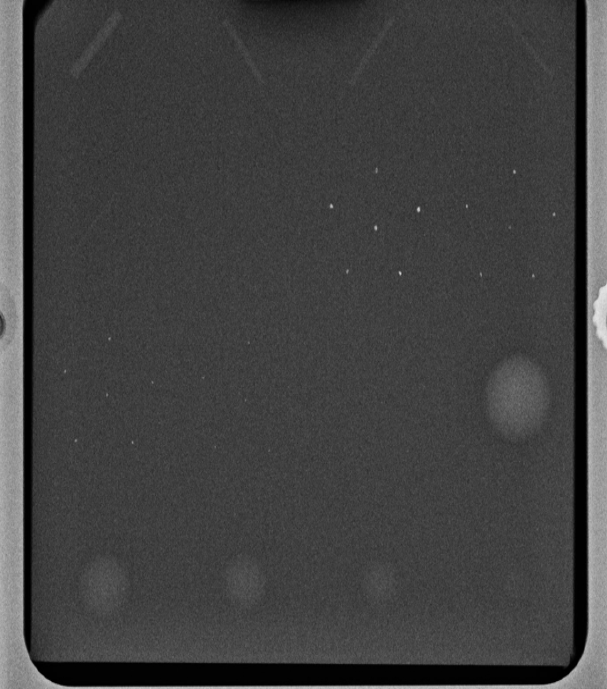
\includegraphics[width=0.5\linewidth]{images/AcrPhantom} 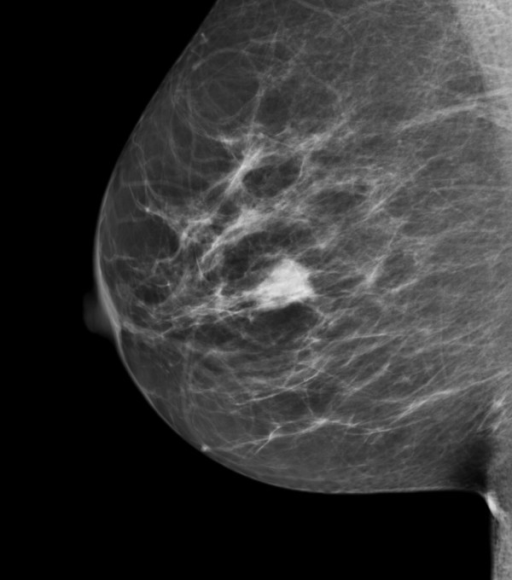
\includegraphics[width=0.5\linewidth]{images/Clinical} \caption{(A) Image of an ACR phantom, (B) Clinical image.}\label{fig:acr-phantom-clinical}
\end{figure}

Fig. \ref{fig:acr-phantom-clinical} (A -- B): (A) Image of an American College of Radiology mammography accreditation phantom. The phantom contains target objects consisting of six fibrils, five groups of microcalcifications, and five nodule-like objects. An image of the phantom is obtained daily, before the first patient is imaged, and is inspected by a technologist, who records the number of target objects of different types that are visible. On his 27'' iMac monitor, I see four fibrils, three speck groups and four masses, which would be graded as a ``pass''. This is greatly simplified version of the test. The scoring accounts for irregular fibril or partially visible masses borders, etc., all of which is intended to get more objectivity out of the measurement. (B) A breast image showing an invasive cancer, located roughly in the middle of the image. Note the lack of similarity between the two images (A) and (B). The breast image is much more complex and there is more information, and therefore more to go wrong than with the phantom image. Moreover, there is variability between patients in contrast to the fixed image in (A). In my clinical experience, the phantom images interpreted visually are a poor predictor of clinical image quality.

One can perhaps appreciate the subjectivity of the measurement. Since the target locations are known, the technologist can claim to have detected it and the claim cannot be disproved; unless a claim is falsifiable, it is not science. While the QC team is trained to achieve repeatable measurements, I have shown TBA {[}30-34{]} that computer analysis of mammography phantom images (CAMPI) can achieve far greater precision and repeatability than human observer readings. Commercial software is currently available from various vendors that perform proprietary analysis of phantom images for various imaging systems (e.g., mammography machines, CT scanners, MRI scanners, ultrasound, etc.).

Fig. \ref{fig:acr-phantom-clinical} (B) shows a mammogram with a mass-like cancer visible near it center. It is characterized by complex anatomical background, quite unlike the uniform background in the phantom image in Fig. \ref{fig:acr-phantom-clinical} (A). In mammography 30\% of retrospectively visible lesions are missed at initial screening and radiologist variability can be as large as 40\% {[}35{]}. QC machine parameters (e.g., kVp, the kilovoltage accuracy) are usually measured to 1\% accuracy. It is ironic that the weak link, in the sense of greatest variability, is the radiologist but quality control and much effort is primarily focused on measuring/improving the physical parameters of the machine. This comment is meant to motivate clinical medical physicists, most of who are focused on QC, to become more aware about observer performance methods, where achieving better than 5\% accuracy is quite feasible{[}36{]}. The author believes there should be greater focus on improving radiologist performance, particularly those with marginal performance. Efforts in this direction, using ROC methods, are underway in the UK {[}37, 38{]} by Prof Alistair Gale and colleagues.

\hypertarget{image-quality-vs.-task-performance}{%
\section{Image quality vs.~task performance}\label{image-quality-vs.-task-performance}}

In this book, ``image quality'' is defined as the fidelity of the image with respect to some external gold standard of what the ideal image should look like, while ``task performance'' is how well a radiologist, using the image, accomplishes a given clinical task. For example, if one had an original Rembrandt and a copy, the image quality of the copy is perfect if even an expert appraiser cannot distinguish it from the original. The original painting is the ``gold standard''. If an expert can distinguish the copy from the original, its image quality is degraded. The amount of degradation is related to the ease with which the expert can detect the fraud.

A radiological image is the result of x-rays interactions within the patient and the image receptor. Here it is more difficult to define a gold standard. If it exists at all, the gold standard is expected to depend on what the image is being used for, i.e., the diagnostic task. An image suitable for soft-tissue disease diagnosis may not be suitable for diagnosis of bone disease. This is the reason why CT scanners have different soft-tissue and bone window/level settings. With clinical images, a frequently used approach is to have an expert rank-order the images, acquired via different methods, with respect to ``clinical appropriateness'' or ``clinical image quality''. The quotes are used to emphasize that these terms are hard to define objectively. In this approach, the gold standard is in the mind of the expert. Since experts have typically interpreted tens of thousands of images in the past, and have lived with the consequences of their decisions, there is considerable merit to using them to judge clinical image quality. However, experts do disagree and biases cannot be ruled out. This is especially true when a new imaging modality is introduced. The initial introduction of computed radiography (CR) was met with some resistance in the US among technologists, who had to learn a different way of obtaining the images that disrupted their workflow. There was also initial resistance from more experienced radiologists, who were uncomfortable with the appearance of the new images, i.e., their gold standard was biased in favor of the modality -- plain films -- that they were most familiar. The author is aware of at least one instance where CR had to be imposed by ``diktat'' from the Chairman of the department. Some of us are more comfortable reading printed material than viewing it on a computer screen, so this type of bias is understandable.

Another source of bias is patient variability, i.e., the gold standard depends on the patient. Some patients are easier to image than others are in the sense that their images are ``cleaner'', i.e., they depict anatomical structures that are known to be present more clearly. X-rays pass readily through a relatively slim patient (e.g., an athlete) and there are fewer scattered photons which degrade image quality{[}39, 40{]}, than when imaging a larger patient (e.g., an NFL linebacker). The image of the former will be clearer, the ribs, the heart shadow, the features of the lungs, etc., will be better visualized (i.e., closer to what is expected based on the anatomy) than the image of the linebacker. Similar differences exist in the ease of imaging women with dense breasts, containing a larger fraction of glandular tissue compared to women with fatty breasts. By imaging appropriately selected patients, one can exploit these facts to make one's favorite imaging system look better. {[}Prof.~Harold Kundel, one of my mentors, used to say: ``Tell me which modality you want to come out better and I will prepare a set of patient images to help you make your case''.{]}

\hypertarget{why-physical-measures-are-not-enough}{%
\section{Why physical measures are not enough}\label{why-physical-measures-are-not-enough}}

Both high spatial resolution and low noise are desirable characteristics. However, imaging systems do not come unambiguously separated as high spatial resolution and low noise vs.~low spatial resolution and high noise. There is generally an intrinsic imaging physics dictated tradeoff between spatial resolution and noise. Improving one makes the other worse. For example, if the digital image is smoothed with, for example, with a spatial filter, then noise will be smaller, because of the averaging of neighboring pixels, but the ability to resolve closely spaced structures will be compromised. Therefore, a more typical scenario is deciding whether the decreased noise justifies the accompanying loss of spatial resolution. Clearly the answer to this depends on the clinical task: if the task is detecting relatively large low contrast nodules, then some spatial smoothing may actually be beneficial, but if the task involves detecting small microcalcifications, often the precursors of cancer in the breast, then the smoothing will tend to reduce their visibility.

The problem with physical measures of image quality lies in relating them to clinical performance. Phantom images have little resemblance to clinical images, compare Fig. \ref{fig:acr-phantom-clinical} (A) and (B). X-ray machines generally have automatic exposure control: the machines use a brief exposure to automatically sense the thickness of the patient from the detected x-rays. Based on this, the machine chooses the best combinations of technical factors (kVp and tube charge) and image processing. The machine has to be put in a special manual override mode to obtain reasonable images of phantoms, as otherwise the exposure control algorithm, which expects patient anatomy, is misled by the atypical nature of the ``patient'', compared to typical patient anatomy, into producing very poor phantom images. This type of problem makes it difficult to reproduce problems encountered using clinical images with phantom images. It has been my general experience that QC failures often lag clinical image quality reported problems: more often than not, clinical image quality problems are reported before QC measurements indicate a problem. This is not surprising since clinical images, e.g., Fig. \ref{fig:acr-phantom-clinical} (B) are more complex and have more information{[}41{]}, both in the clinical and in the information theoretic sense{[}42{]}, than the much simpler phantom image shown in Fig. \ref{fig:acr-phantom-clinical} (A), so there is more that can go wrong with clinical images than with phantom images. Manufacturers now design anthropomorphic phantoms whose images resemble human x-rays. Often these phantoms provide the option of inserting target objects at random locations; this is desired to get more objectivity out of the measurement. Now, if the technologist claims to have found the target, the indicated location can be used to determine if the target was truly detected.

To circumvent the possibility that changes in physical measurements on phantoms may not sensitively track changes in clinical image interpretations by radiologists, a measurement needs to include both the complexity of clinical images and radiologists as part of the measurement. Because of variability in both patient images and radiologist interpretations, such measurements are expected to be more complicated than QC measurements, so to be clear, I am not advocating observer performance studies as part of QC. However, they could be built into a continuous quality improvement program, perhaps performed annually. Before giving an outline of the more complex methods, an alternative modeling driven approach, that is widely used, is described next.

\hypertarget{model-observers}{%
\section{Model observers}\label{model-observers}}

If one can adequately simulate (or model) the entire imaging process, then one can design mathematical measurements that can be used to decide if a new imaging system is an improvement over a conventional imaging system. Both new and conventional systems are modeled (i.e., reduced to formulae that can be evaluated). The field of model-observers{[}43{]} is based on assuming this can be done. The FDA/CDRH has a research program called VICTRE: Virtual Imaging Clinical Trials for Regulatory Evaluation. Since everything is done on a computer, the method does not require time-consuming studies involving radiologists.

A simple example may elucidate the process (for more details one should consult the extensive literature on model-observers). Suppose one simulates image noise by sampling a Gaussian random number generator and filling up the pixels in the image with the random samples. This simulates a non-diseased image. The number of such images could be quite large, e.g., 1000, limited only by one's patience. A second set of simulated diseased images is produced in which one samples a random number generator to create non-diseased images, as before, but this time one adds a small low-contrast but noiseless disk, possibly with Gaussian edges, to the center of each image. The procedure yields two sets of images, 1000 with noise only backgrounds and 1000 with different noise backgrounds and the superposed centered low contrast disk. One constructs a template whose shape is identical to that of the superposed disk (i.e., one does not simply measure peak contrast at the center of the lesion; rather the shape-dependent contrast of the disk is taken into account). One then calculates the cross-correlation of the template with each of the superposed disks{[}30, 44{]}. The cross correlation is the sum of the products of pixel values of corresponding pixels, one drawn from the template and the other drawn from the matching position on the disk image. {[}Details of this calculation are in Online Appendix 12.B of Chapter 12.{]} Because of random noise, the cross-correlations from different simulated diseased cases will not be identical, and one averages the 1000 values. Next one applies the template to the centers of the non-diseased images and computes the cross correlations as before. Because of the absence of the disk, the values will be smaller (assuming positive disk contrast). The difference between the average of the cross-correlations at disk locations and the average at disk-absent locations is the numerator of a signal to noise ratio (SNR) like quantity. The denominator is the standard deviation of the cross-correlations at disk-free locations. To be technical, the procedure yields the signal-to-noise-ratio (SNR) of the non-pre-whitening ideal observer{[}45{]}. It is an ideal mathematical ``observer'' in the sense that for white noise no human observer can surpass this level of performance{[}46, 47{]}.

Suppose the task is to evaluate two image-processing algorithms. One applies each algorithm to the 2000 images described above and measures SNR for each algorithm. The one yielding the higher SNR, after accounting for variability in the measurements, is the superior algorithm.

Gaussian noise images are not particularly ``clinical'' in appearance. If one filters the noise appropriately, one can produce simulated images that are similar to non-diseased backgrounds observed in mammography{[}48-50{]}. Other techniques exist for simulating statistically characterized lumpy backgrounds that are a closer approximation to some medical images{[}51{]}.

Having outlined one of the alternatives, one is ready for the methods that form the subject matter of this book.

\hypertarget{measuring-observer-performance-four-paradigms}{%
\section{Measuring observer performance: four paradigms}\label{measuring-observer-performance-four-paradigms}}

Observer performance measurements come in different ``flavors'', types or paradigms. In the current context, a paradigm is an agreed-upon method for collecting the data. A given paradigm can lend itself to different analyses. In historical order the paradigms are: (1) the receiver operating characteristic (ROC) paradigm {[}1, 2, 7, 52, 53{]}; (2) the free-response ROC (FROC) paradigm {[}54, 55{]}; (3) the location ROC (LROC) paradigm {[}56, 57{]} and (4) the region of interest (ROI) paradigm {[}58{]}. Each paradigm assumes that the truth is known independently of the modalities to be compared. This implies that one cannot use diagnoses from one of the modalities to define truth -- if one did, the measurement would be biased in favor of the modality used to define truth. It is also assumed that the true disease status of the image is known to the researcher but the radiologist is ``blinded'' to this information.

In the ROC paradigm the observer renders a single decision per image. The decision could be communicated using a binary scale (ex. 0 or 1) or declared by use of the terms ``negative'' or ``positive,'' abbreviations of ``negative for disease'' (the radiologist believes the patient is non-diseased) and ``positive for disease'' (the radiologist believes the patient is diseased), respectively. Alternatively, the radiologist could give an ordered numeric label, termed a rating, to each case where the rating is a number with the property that higher values correspond to greater radiologist's confidence in presence of disease. A suitable ratings scale could be the consecutive integers 1 through 6, where ``1'' is ``definitely non-diseased'' and ``6'' is ``definitely diseased''.

If data is acquired on a binary scale, then the performance of the radiologist can be plotted as a single operating point on an ROC plot. The x-axis of the plot is false positive fraction (FPF), i.e., the fraction of non-diseased cases incorrectly diagnosed as diseased. The y-axis of the plot is true positive fraction (TPF), i.e., the fraction of diseased cases correctly diagnosed as diseased. Models have been developed to fit binary or multiple rating datasets. These models predict continuous curves, or operating characteristics, along which an operating point can move by varying the radiologist's reading style. The reading style is related to the following concept: based on the evidence in the image, how predisposed is a radiologist to declaring a case as diseased. A ``lenient'', ``lax'' or ``liberal'' reporting style radiologist is very predisposed even with scant evidence. A ``strict'' or ``conservative'' reporting style radiologist requires more evidence before declaring a patient as diseased. This brief introduction to the ROC was given to explain the term ``operating characteristic'' in ROC. The topic is addressed in more detail in Chapter 02.

In the FROC paradigm the observer marks and rates all regions in the image that are sufficiently suspicious for disease. A mark is the location of the suspicious region and the rating is an ordered label, characterizing the degree of suspicion attached to the suspicious region. In the LROC paradigm the observer gives an overall ROC-type rating to the image, and indicates the location of the most suspicious region in the image. In the ROI paradigm the researcher divides each image into a number of adjacent non-overlapping regions of interest (ROIs) that cover the clinical area of interest. The radiologist's task is to evaluate each ROI for presence of disease and give an ROC-type rating to it.

\hypertarget{basic-approach-to-the-analysis}{%
\subsection{Basic approach to the analysis}\label{basic-approach-to-the-analysis}}

The basic approach is to obtain data, according to one of the above paradigms, from a group of radiologists interpreting a common set of images in one or more modalities. The way the data is collected, and the structure of the data, depends on the selected paradigm. The next step is to adopt an objective measure of performance, termed a figure or merit (FOM) and a procedure for estimating it for each modality-reader combination. Assuming two modalities, e.g., a new modality and the conventional one, one averages FOM over all readers within each modality. If the difference between the two averages (new modality minus the conventional one) is positive, that is an indication of improvement. Next comes the statistical part: is the difference large enough so as to be unlikely to be due to chance. This part of the analysis, termed significance testing, yields a probability, or p-value, that the observed difference or larger could result from chance even though the modalities have identical performances. If the p-value is very small, that it is taken as evidence that the modalities are not identical in performance, and if the difference is in the right direction, the new modality is judged better.

\hypertarget{historical-notes}{%
\subsection{Historical notes}\label{historical-notes}}

The term ``receiver operating characteristic'' (ROC) traces its roots to the early 1940s. The ``receiver'' in ROC literally denoted a pulsed radar receiver that detects radio waves bounced off objects in the sky, the obvious military application being to detect enemy aircraft. Sometimes the reflections were strong compared to receiver electronic noise and other sources of noise and the operator could confidently declare that the reflection indicated the presence of aircraft and the operator was correct. This combination of events was termed a true positive (TP). At other times the aircraft was present but due to electronic noise and reflections off clouds, the operator was not confident enough to declare ``aircraft present'' and this combination of events was termed a false negative (FN). Two other types of decisions can be discerned when there was no aircraft in the field of view: (1) the operator mistook reflections from clouds or perhaps a flock of large birds and declared ``aircraft present'', termed a false positive (FP). (2) The operator did not declare ``aircraft present'' because the reflected image was clear of noise or false reflections and the operator felt confident in a negative decision, termed a true negative (TN). Obviously, it was desirable to maximize correct decisions (TPs and TNs) while minimizing incorrect decisions (FNs and FPs). Scientists working on this problem analyzed it as a generic signal detection problem, where the signal was the aircraft reflection and the noise was everything else. A large field called signal detection theory (SDT) emerged{[}59{]}. However, even at this early stage, it must have been apparent to the researchers that the problem was incomplete in a key respect: when the operator detects a suspicious signal, there is a location (specifically an azimuth and altitude associated with it. The operator could be correct in stating ``aircraft present'' but direct the interceptors to the wrong location. Additionally, there could be multiple enemy aircraft present, but the operator is only allowed the ``aircraft present'' and ``aircraft absent'' responses, which fail to allow for multiplicity of suspected aircraft locations. This aspect was not recognized, to the best of my knowledge, until Egan coined the term ``free-response'' in the auditory detection context{[}54{]}.

Having briefly introduced the different paradigms, two of which, namely the ROC and the FROC, will be the focus of this book, it is appropriate to see how these measurements fit in with the different types of measurements possible in assessing imaging systems.

\hypertarget{hierarchy-of-assessment-methods}{%
\section{Hierarchy of assessment methods}\label{hierarchy-of-assessment-methods}}

The methods described in this book need to be placed in context of a six-level hierarchy of assessment methods\citep[\citet{fryback1991efficacy}]{kundel2008receiver}. The term efficacy is defined generically as ``the probability of benefit to individuals in a defined population from a medical technology applied for a given medical problem under ideal conditions of use''. Demonstration of efficacy at each lower level is a necessary but not sufficient condition to assure efficacy at higher level. The different assessment methods are, in increasing order of efficacy : technical, diagnostic accuracy, diagnostic thinking, therapeutic, patient outcome and societal, Table \ref{tab:fryback-thornbury}.

Table \ref{tab:fryback-thornbury}: Fryback and Thornbury proposed hierarchy of assessment methods. Demonstration of efficacy at each lower level is a necessary but not sufficient condition to assure efficacy at higher level. {[}MTF = modulation transfer function; NPS(f) = noise power spectra as a function of spatial frequency f; DQE(f) = detective quantum efficiency{]}

\begin{table}

\caption{\label{tab:fryback-thornbury}Fryback Thornbury hierarchy of efficacies.}
\centering
\begin{tabular}[t]{l|l}
\hline
Level Designation & Essential Characteristic\\
\hline
1. Technical efficacy & Engineering measures: MTF, NPS, DQE\\
\hline
2. Diagnostic accuracy efficacy & Sensitivity, specificity, ROC or FROC area\\
\hline
3. Diagnostic thinking efficacy & Positive and negative predictive values\\
\hline
4. Therapeutic efficacy & Treatment benefits from imaging test?\\
\hline
5. Patient outcome efficacy & Patients benefit from imaging test?\\
\hline
6. Societal efficacy & Society benefits from imaging test?\\
\hline
\end{tabular}
\end{table}

The term ``clinical relevance'' is used rather loosely in the literature. The author is not aware of an accepted definition of ``clinical relevance'' apart from its obvious English language meaning. As a working definition I have proposed {[}63{]} that the clinical relevance of a measurement be defined as its hierarchy-level. A level-5 patient outcome measurement (do patients, on the average, benefit from the imaging study) is clinically more relevant than a technical measurement like noise on a uniform background phantom or an ROC study. This is because it relates directly to the benefit, or lack thereof, to a group of patients (it is impossible to define outcome efficacy at the individual patient level -- at the patient level outcome is a binary random variable, e.g., 1 if the outcome was good or 0 if the outcome was bad).

One could make physical measurements ad-infinitum, but one cannot (yet) predict the average benefit to patients. Successful virtual clinical trials would prove me wrong. ROC studies are more clinically relevant than physical measurements, and it is more likely that a modality with higher performance will yield better outcomes, but it is not a foregone conclusion. Therefore, higher-level measurements are needed.

However, the time and cost of the measurement increases rapidly with the hierarchy level. Technical efficacy, although requiring sophistical mathematical methods, take relatively little time. ROC and FROC, both of which are level-2 diagnostic accuracy measurements, take more time, often a few months to complete. However, since ROC measurements include the entire imaging chain and the radiologist, they are more clinically relevant than technical measurements, but they do not tell us the effect on diagnostic thinking. After the results of ``live'' interpretations are available, e.g., patients are diagnosed as diseased or non-diseased, what does the physician do with the information. Does the physician recommend further tests or recommends immediate treatment. This is where the level-3 measurements come in, which measure the effect on diagnostic thinking. Typical level-3 measurements are positive predictive value (PPV) and negative predictive value (NPV). PPV is the probability that the patient is actually diseased when the diagnosis is diseased and NPV is the probability that the patient is actually non-diseased when the diagnosis is non-diseased. These are discussed in more detail in Chapter 02.

Unlike level-2 measurements, PPV and NPV depend on disease prevalence. As an example consider breast cancer which (fortunately) has low prevalence, about 0.005. Before the image is interpreted and lacking any other history, the mammographer knows only there is a five in 1000 chance that the woman has breast cancer. After the image is interpreted, the mammographer has more information. If the image was interpreted as diseased, the confidence in presence of cancer increases. For an expert mammographer typical values of sensitivity and specificity are 80\% and 90\%, respectively (these terms will be explained in the next chapter; sensitivity is identical to true positive fraction and specificity is 1-false positive fraction). It will be shown (in Chapter 02, §2.9.2) that for this example PPV is only 0.04. In other words, even though an expert interpreted the screening mammogram as diseased, the chance that the patient actually has cancer is only 4\%. Obviously more tests are needed before one knows for sure if the patient has cancer -- this is the reason for the recall and the subsequent diagnostic workup referred to in §1.2.2. The corresponding NPV is 0.999. Negative interpretations by experts are definitely good news for the affected patients and these did not come directly from an ROC study, or physical measurements, rather they came from actual ``live'' clinical interpretations. Again, NPV and PPV are defined as averages over a group of patients. For example, the 4\% chance of cancer following a positive diagnosis is good news, on the average. An unlucky patient could be one of the four-in-100-patients that has cancer following a positive screening diagnosis.

While more relevant than ROC, level-3 measurements like PPV and NPV are more difficult to conduct than ROC studies {[}18{]} -- they involve following, in real time, a large cohort of patients with images interpreted under actual clinical conditions. Level 4 and higher measurements, namely therapeutic, patient outcome and societal, are even more difficult and are sometimes politically charged, as they involve cost benefit considerations.

\hypertarget{overview-of-the-book-and-how-to-use-it}{%
\section{Overview of the book and how to use it}\label{overview-of-the-book-and-how-to-use-it}}

For the most part the book follows the historical development, i.e., it starts with chapters on ROC methodology, chapters on significance testing, chapters on FROC methodology, chapters on advanced topics and appendices. Not counting Chapter 01, the current chapter, the book is organized five Parts (A - E).

\hypertarget{overview-of-the-book}{%
\subsection{Overview of the book}\label{overview-of-the-book}}

\hypertarget{part-a-the-roc-paradigm}{%
\subsubsection{Part A: The ROC paradigm}\label{part-a-the-roc-paradigm}}

Part A describes the ROC (receiver operating characteristic) paradigm. Chapter 02 describes the binary decision task. Terminology that is important to master, such as accuracy, sensitivity, specificity, disease prevalence, positive and negative predictive values is introduced. Chapter 03 introduces the important concepts of decision variable, the reporting threshold, and how the latter may be manipulated by the researcher and it introduces the ROC curve. Chapter 04 reviews the widely used ratings method for acquiring ROC data. Chapter 06 introduces the widely used binormal model for fitting ratings data. The chapter is heavy on mathematical and computational aspects, as it is intended to take the mystery out of these techniques, which are used in subsequent chapters. The data fitting method, pioneered by Dorfman and Alf in 1969, is probably one of the most used algorithms in ROC analysis. Chapter 07 describes sources of variability affecting any performance measure, and how they can be estimated.

\hypertarget{part-b-the-statistics-of-roc-analysis}{%
\subsubsection{Part B: The statistics of ROC analysis}\label{part-b-the-statistics-of-roc-analysis}}

Part B describes the specialized statistical methods needed to analyze ROC data, in particular how to analyze data originating from multiple readers interpreting the same cases in multiple modalities. Chapter 08 introduces hypothesis-testing methodology, familiar to statisticians, and the two types of errors that the researcher wishes to control, the meaning of the ubiquitous p-value and statistical power. Chapter 09 focuses on the Dorfman-Berbaum-Metz method, with improvements by Hillis. Relevant formulae, mostly from publications by Prof.~Steven Hillis, are reproduced without proofs (it is my understanding that Dr.~Hillis is working on a book on his specialty, which should nicely complement the minimalistic-statistical description approach adopted in this book). Chapter 10 describes the Obuchowski-Rockette method of analyzing MRMC ROC data, with Hillis' improvements. Chapter 11 describes sample size estimation in an ROC study.

\hypertarget{part-c-the-froc-paradigm}{%
\subsubsection{Part C: The FROC paradigm}\label{part-c-the-froc-paradigm}}

Part C is unique to this book. Anyone truly wishing to understand human observer visual search performance needs to master it. The payoff is that the concepts, models and methods described here apply to almost all clinical tasks. Chapter 17 and Chapter 18 are particularly important. These were difficult chapters to write and they will take extra effort to comprehend. However, the key findings presented in these chapters and their implications should strongly influence future observer performance research. If the potential of the findings is recognized and used to benefit patients, by even one reader, I will consider this book a success. Chapter 19 describes how to analyze FROC data and report the results.

\hypertarget{part-d-advanced-topics}{%
\subsubsection{Part D: Advanced topics}\label{part-d-advanced-topics}}

Some of the chapters in Part D are also unique to this book. Chapter 20 discusses proper ROC curve fitting and software. The widely used bivariate binormal model, developed around 1980, but never properly documented, is explained in depth, and a recent extension of it that works with any dataset is described in Chapter 21. Also described is a method for comparing (standalone) CAD to radiologists, Chapter 22. Standalone CAD performance is rarely measured, which is a serious mistake, for which we are all currently paying the price. It does not work for masses in mammography{[}64-66{]}. In the UK CAD is not used, instead they rely on double readings by experts, which is actually the superior approach, given the current low bar used in the US for CAD to be considered a success. Chapter 23, co-authored by Mr.~Xuetong Zhai, a graduate student, describes validation of the CAD analysis method described in Chapter 22. It describes constructing a single-modality multiple-reader ratings data simulator. The method is extendible to multiple-modality multiple-reader datasets.

\hypertarget{how-to-use-the-book}{%
\subsection{How to use the book}\label{how-to-use-the-book}}

Those new to the field should read the chapters in sequence. It is particularly important to master Part A. Part B presents the statistical analysis at a level accessible to the expected readers of this book, namely the user community. The only way to really understand this part is to apply the described methods and codes to the online datasets. Understanding the formulae in this part, especially those relating to statistical hypothesis testing, requires statistical expertise, which could lead the average reader in unproductive directions. It is best to accept the statisticians' formulae and confirm that they work.

\hypertarget{overview-Summary}{%
\section{Summary}\label{overview-Summary}}

\hypertarget{overview-Discussion}{%
\section{Discussion}\label{overview-Discussion}}

\hypertarget{overview-references}{%
\section{Chapter References}\label{overview-references}}

\hypertarget{part-roc-paradigm}{%
\part*{ROC paradigm}\label{part-roc-paradigm}}
\addcontentsline{toc}{part}{ROC paradigm}

\hypertarget{binary-task}{%
\chapter{The Binary Task}\label{binary-task}}

\hypertarget{binary-task-how-much-finished}\label{binary-task-how-much-finished}}

\hypertarget{binary-taskIntro}{%
\section{Introduction}\label{binary-taskIntro}}

In the previous chapter four observer performance paradigms were introduced: the receiver operating characteristic (ROC), the free-response ROC (FROC), the location ROC (LROC) and the region of interest (ROI). The next few chapters focus on the ROC paradigm, where each case is rated for confidence in presence of disease. While a multiple point rating scale is generally used, in this chapter it is assumed that the ratings are binary, and the allowed values are ``1'' vs.~``2''. Equivalently, the ratings could be ``non-diseased'' vs.~``diseased'', ``negative'' vs.~``positive'', etc. In the literature this method of data acquisition is also termed the ``yes/no'' procedure \citep{green1966signal, egan1975book}. The reason for restricting, for now, to the binary task is that the multiple rating task can be shown to be equivalent to a number of simultaneously conducted binary tasks. Therefore, understanding the simpler method is a good starting point.

Since the truth is also binary one can define a 2 x 2 table summarizing the outcomes in such studies and useful fractions that can be defined from the counts in this table, the most important ones being true positive fraction (TPF) and false positive fraction (FPF). These are used to construct measures of performance, some of which are desirable from the researcher's point of view, but others are more relevant to radiologists. The concept of disease prevalence is introduced and used to derive relations between the different types of measures. An \texttt{R} example of calculation of these quantities is given.

\hypertarget{binary-task-2-2-table}{%
\section{The 2x2 table}\label{binary-task-2-2-table}}

In this book, the term ``case'' is used for images obtained for diagnostic purposes, of a patient; often multiple images of a patient, sometimes from different modalities, are involved in an interpretation; all images of a single patient that are used in the interpretation are collectively referred to as a case. A familiar example is the 4-view presentation used in screening mammography, where two views of each breast are viewed.

Let \(\text{D}\) represent the radiologist's decision with \(\text{D}=1\) representing the decision ``case is diagnosed as non-diseased'' and \(\text{D}=2\) representing the decision ``case is diagnosed as diseased''. Let \(\text{T}\) denote the truth with \(\text{T}=1\) representing ``case is actually non-diseased'' and \(\text{T}=2\) representing ``case is actually diseased''. Each decision, one of two values, will be associated with one of two truth states, resulting in an entry in one of 4 cells arranged in a 2 x 2 layout, termed the decision vs.~truth table, Table \ref{tab:binary-task-truth-table} which is of fundamental importance in observer performance. The cells are labeled as follows. The abbreviation \(\text{TN}\), for true negative, represents a \(\text{D}=1\) decision on a \(\text{T}=1\) case. \(\text{FN}\), for false negative, represents a \(\text{D}=1\) decision on a \(\text{T}=2\) case (also termed a ``miss''). \(\text{FP}\), for false positive, represents a \(\text{D}=2\) decision on a \(\text{T}=1\) case (a ``false-alarm'') and \(\text{TP}\), for true positive, represents a \(\text{D}=2\) decision on a \(\text{T}=2\) case (a ``hit'').

\begin{table}

\caption{\label{tab:binary-task-truth-table}Truth Table.}
\centering
\begin{tabular}[t]{l|l|l}
\hline
  & T=1 & T=2\\
\hline
D=1 & TN & FN\\
\hline
D=2 & FP & TP\\
\hline
\end{tabular}
\end{table}

Table \ref{tab:binary-task-truth-table2} shows the number of decisions in each of the four categories defined in Table \ref{tab:binary-task-truth-table}. \(n(\text{TN})\) is the number of true negative decisions, \(n(\text{FN})\) is the number of false negative decisions, etc. The last row is the sum of the corresponding columns. The sum of the number of true negative decisions \(n(\text{TN})\) and the number of false positive decisions \(n(\text{FP})\) must equal the total number of non-diseased cases, denoted \(K_1\). Likewise, the sum of the number of false negative decisions \(n(\text{FN})\) and the number of true positive decisions \(n(\text{TP})\) must equal the total number of diseased cases, denoted \(K_2\). The last column is the sum of the corresponding rows. The sum of the number of true negative \(n(\text{TN})\) and false negative \(n(\text{FN})\) decisions is the total number of negative decisions, denoted \(n(N)\). Likewise, the sum of the number of false positive \(n(\text{FP})\) and true positive \(n(\text{TP})\) decisions is the total number of positive decisions, denoted \(n(P)\). Since each case yields a decision, the bottom-right corner cell is \(n(N) + n(P)\), which must also equal \(K_1+K_2\), the total number of cases denoted \(K\). These statements are summarized in Eqn. \eqref{eq:binary-task-truth-table-eqns}.

\begin{equation} 
\left.
\begin{aligned}
K_1&=n(TN)+n(FP)\\ 
K_2&=n(FN)+n(TN)\\ 
n(N)&=n(TN)+n(FN)\\ 
n(P)&=n(TP)+n(FP)\\
K=K_1+K_2&=n(N)+n(P)
\end{aligned}
\right\}
\label{eq:binary-task-truth-table-eqns}
\end{equation}

\begin{table}

\caption{\label{tab:binary-task-truth-table2}Individual 2x2 table cell counts and row and column sums. $K_1$ is the number of non-diseased cases, $K_2$ is the number of diseased cases and $K$ is the total number of cases. }
\centering
\begin{tabular}[t]{l|l|l|l}
\hline
  & T=1 & T=2 & RowSums\\
\hline
D=1 & n(TN) & n(FN) & n(N)=n(TN)+n(FN)\\
\hline
D=2 & n(FP) & n(TP) & n(P)=n(FP)+n(TP)\\
\hline
ColSums & $K_1$=n(TN)+n(FP) & $K_2$=n(FN)+n(TP) & $K=K_1+K_2$=n(N)+n(P)\\
\hline
\end{tabular}
\end{table}

\hypertarget{sensitivity-and-specificity}{%
\section{Sensitivity and specificity}\label{sensitivity-and-specificity}}

The notation \(\text{P(D|T)}\) indicates the probability of diagnosis \(\text{D}\) for a given truth state \(\text{T}\). The vertical bar is used to denote a conditional probability, i.e., the probability of what is to the left of the bar occurring when what is to the right of the bar is true:

\begin{equation} 
\text{P(D|T)} \equiv P(\text{diagnosis is D} | \text{truth is T})
\label{eq:binary-task-p-d-given-t}
\end{equation}

Therefore the probability that the radiologist will diagnose ``case is diseased'' when the case is actually diseased is \(\text{P(D=2|T=2)}\), the probability of a true positive \(\text{P(TP)}\).

\begin{equation} 
\text{P(TP)} = \text{P(D = 2 | T = 2)}
\label{eq:binary-task-p-tp}
\end{equation}

Likewise, the probability that the radiologist will diagnose ``case is non-diseased'' when the case is actually diseased is \(\text{P(D=1|T=2)}\), the probability of a false negative \(\text{P(FN)}\).

\begin{equation} 
\text{P(FN)} = \text{P(D = 1 | T = 2)}
\label{eq:binary-task-p-fn}
\end{equation}

The corresponding probabilities for non-diseased cases, \(P(TN)\) and \(P(FP)\), are defined by:

\begin{equation} 
\left.
\begin{aligned}
\text{P(TN)}&=\text{P(D=1|T=1)}\\ 
\text{P(FP)}&=\text{P(D=2|T=1)}
\end{aligned}
\right\}
\label{eq:binary-task-p-tn-fp}
\end{equation}

Since the diagnosis must be either \(D=1\) or \(D=2\), the following must be true:

\begin{equation} 
\left.
\begin{aligned}  
\text{P(D=1|T=1)+P(D=2|T=1)}=&1\\ 
\text{P(D=1|T=2)+P(D=2|T=2)}=&1
\end{aligned}
\right \}
\label{eq:binary-task-p-sum-to-unity}
\end{equation}

Equivalently, these equations can be written:

\begin{equation} 
\left.
\begin{aligned}  
\text{P(TN)+P(FP)}=& 1\\ 
\text{P(FN)+P(TP)}=& 1
\end{aligned}
\right \}
\label{eq:binary-task-p-sum-to-unity2}
\end{equation}

Comments:

\begin{itemize}
\item
  An easy way to remember Eqn. \eqref{eq:binary-task-p-sum-to-unity2} is to start by writing down one of the four probabilities, e.g., \(\text{P(TN)}\), and ``reversing'' both terms inside the parentheses, i.e., \(\text{T} \Rightarrow \text{F}\), and \(\text{N} \Rightarrow \text{P}\). This yields the term \(\text{P(FP)}\) which when added to the previous probability yields unity, i.e., the first equation in Eqn. \eqref{eq:binary-task-p-sum-to-unity2}.
\item
  Because there are two equations in four unknowns, only two of the four probabilities are independent. By tradition these are chosen to be \(\text{P(D=1|T=1)}\) and \(\text{P(D=2|T=2)}\), i.e., \(P(TN)\) and \(P(TP)\), the probabilities of correct decisions on non-diseased and diseased cases, respectively. The two basic probabilities are so important that they have names: \(\text{P(D=2|T=2)=P(TP)}\) is termed \textbf{sensitivity} (Se) and \(\text{P(D=1|T=1)=P(TN)}\) is termed \textbf{specificity} (Sp):
\end{itemize}

\begin{equation} 
\left.
\begin{aligned}  
\text{Se}=\text{P(TP)=P(D=2|T=2)}\\ 
\text{Sp}=\text{P(TN)=P(D=1|T=1)}
\end{aligned}
\right \}
\label{eq:binary-task-se-sp}
\end{equation}

\begin{quote}
The radiologist can be regarded as a diagnostic-test yielding a binary decision under the binary truth condition. More generally, any test (e.g., a blood test for HIV) yielding a binary result (positive or negative) under a binary truth condition is said to be sensitive if it correctly detects the diseased condition most of the time. The test is said to be specific if it correctly detects the non-diseased condition most of the time. Sensitivity is how correct the test is at detecting a diseased condition, and specificity is how correct the test is at detecting a non-diseased condition.
\end{quote}

\hypertarget{estimating-sensitivity-and-specificity}{%
\subsection{Estimating sensitivity and specificity}\label{estimating-sensitivity-and-specificity}}

Sensitivity and specificity are the probabilities of correct decisions over diseased and non-diseased cases, respectively. The true values of these probabilities would require interpreting all diseased and non-diseased cases in the entire population of cases. In reality, one has a finite sample of cases and the corresponding quantities, calculated from this finite sample, are termed \textbf{estimates}. Population values are fixed, and in general unknown, while estimates are realizations of random variables. Intuitively, an estimate calculated over a larger number of cases is expected to be closer to the population value than an estimate calculated over a smaller number of cases.

Estimates of sensitivity and specificity follow from counting the numbers of TP and TN decisions in Table \ref{tab:binary-task-truth-table2} and dividing by the appropriate denominators. For sensitivity, the denominator is the number of diseased cases \(K_2\) and for specificity, the appropriate denominator is the number of non-diseased cases \(K_1\). The estimation equations for sensitivity specificity are (estimates are often denoted by the ``hat'' or circumflex symbol \^{}):

\begin{equation} 
\left.
\begin{aligned}  
\widehat{\text{Se}}=\widehat{\text{P(TP)}}=\frac{\text{n(TP)}}{K_2}\\
\widehat{\text{Sp}}=\widehat{\text{P(TN)}}=\frac{\text{n(TN)}}{K_1}
\end{aligned}
\right \}
\label{eq:binary-task-se-sp-est}
\end{equation}

\begin{quote}
The ratio of the number of TP decisions to the number of actually diseased cases is termed \textbf{true positive fraction} \(\widehat{\text{TPF}}\), an estimate of sensitivity, or equivalently an estimate of \(\widehat{\text{P(TP)}}\). Likewise, the ratio of the number of TN decisions to the number of actually non-diseased cases is termed \textbf{true negative fraction} \(\widehat{\text{TNF}}\), an estimate of specificity, or equivalently an estimate of \(\widehat{\text{P(TN)}}\). The complements of \(\widehat{\text{TPF}}\) and \(\widehat{\text{TNF}}\) are termed \textbf{false negative fraction} \(\widehat{\text{FNF}}\) and \textbf{false positive fraction} \(\widehat{\text{FPF}}\), respectively.
\end{quote}

\hypertarget{disease-prevalence}{%
\section{Disease prevalence}\label{disease-prevalence}}

Disease prevalence, often abbreviated to prevalence, is defined as the probability that a randomly sampled case is of a diseased patient, i.e., the fraction of the entire population that is diseased. It is denoted \(\text{P(D|pop)}\) when patients are randomly sampled from the population (``pop'') and otherwise it is denoted \(\text{P(D|lab)}\), where the condition ``lab'' stands for a laboratory study, where cases may be artificially enriched, and thus not representative of the population:

\begin{equation} 
\left.
\begin{aligned}  
P(\text{D}|\text{pop})=&P(\text{T}=2|\text{pop})\\
P(\text{D}|\text{lab})=&P(\text{T}=2|\text{lab})
\end{aligned}
\right \}
\label{eq:binary-task-dis-prev}
\end{equation}

Since the patients must be either diseased on non-diseased it follows with either sampling method that:

\begin{equation} 
\left.
\begin{aligned}  
P(\text{T}=1|\text{pop})+P(\text{T}=2|\text{pop})&=1\\
P(\text{T}=1|\text{lab})+P(\text{T}=2|\text{lab})&=1
\end{aligned}
\right \}
\end{equation}

If a finite number of patients are sampled randomly from the population the fraction of diseased patients in the sample is an estimate of true disease prevalence.

\begin{equation} 
\left.
\begin{aligned}  
\widehat{P(\text{D}|\text{pop})}=
\frac{K_2}{K_1+K_2}
\end{aligned}
\right \}
\label{eq:binary-task-dis-prev-est}
\end{equation}

It is important to appreciate the distinction between population prevalence and the laboratory prevalence. As an example true disease prevalence for breast cancer is about five per 1000 patients in the US, but most mammography studies are conducted with comparable numbers of non-diseased and diseased cases:

\begin{equation} 
\left.
\begin{aligned}  
\widehat{P(\text{D}|\text{pop})}\sim& 0.005\\
\widehat{P(\text{D}|\text{lab})}\sim& 0.5\gg \widehat{P(\text{D}|\text{pop})}
\end{aligned}
\right \}
\label{eq:binary-task-dis-prev-lab-vs-pop}
\end{equation}

\hypertarget{accuracy}{%
\section{Accuracy}\label{accuracy}}

Accuracy is defined as the fraction of all decisions that are correct. Denoting it by \(\text{Ac}\) one has for the corresponding estimate:

\begin{equation} 
\widehat{\text{Ac}}=\frac{n(TN)+n(TP)}{n(TN)+n(TP)+n(FP)+n(FN)}
\label{eq:binary-task-ac-est}
\end{equation}

Explanation: the numerator is the total number of correct decisions and the denominator is the total number of decisions. An equivalent expression is:

\begin{equation} 
\widehat{\text{Ac}}=\widehat{\text{Sp}}\widehat{P(!D)}+\widehat{\text{Se}}\widehat{P(D)}
\label{eq:binary-task-ac-est2}
\end{equation}

The exclamation mark symbol is used to denote the ``not'' or negation operator. For example, \(P(!D)\) means the probability that the patient is not diseased. Eqn. \eqref{eq:binary-task-ac-est2} applies equally to laboratory or population studies, \emph{provided sensitivity and specificity are estimated consistently}. One cannot, for example, combine a population estimate of prevalence with a laboratory estimate of sensitivity.

Eqn. \eqref{eq:binary-task-ac-est2} can be understood from the following argument. \(\widehat{Sp}\) is the fraction of correct decisions on non-diseased cases. Multiplying this by \(\widehat{P(!D)}\) yields the fraction of correct negative decisions on all cases. Similarly \(\widehat{Se}\) is the fraction of correct decisions on diseased cases. Multiplying this by \(\widehat{P(D)}\) yields the fraction of correct positive decisions on all cases. Their sum is the fraction of correct decisions on all cases.

A formal mathematical derivation follows: Eqn. \eqref{eq:binary-task-se-sp} yields:

\begin{equation} 
\left.
\begin{aligned}  
n(TP)=K_2 \widehat{Se}\\ 
n(TN)=K_1 \widehat{Sp}
\end{aligned}
\right \}
\label{eq:binary-task-ntp-ntn}
\end{equation}

Therefore,

\begin{equation} 
\left.
\begin{aligned}  
\widehat{Ac}&=\frac{n(TN)+n(TP)}{K}\\
&=\frac{K_1 \widehat{Sp}+K_2 \widehat{Se}}{K}\\
&=\widehat{Sp} \widehat{P(!D)}+\widehat{Se}\widehat{P(D)}
\end{aligned}
\right \}
\label{eq:binary-task-ac}
\end{equation}

For the population one can dispense with the carets:

\begin{equation} 
\left.
\begin{aligned}  
\text{Ac}&=\frac{n(TN)+n(TP)}{K}\\
&=\frac{K_1 \text{Sp}+K_2 \text{Se}}{K}\\
&=\text{Sp} \text{P(!D)}+\text{Se}\widehat{P(D)}
\end{aligned}
\right \}
\label{eq:binary-task-ac-pop}
\end{equation}

\hypertarget{negative-and-positive-predictive-values}{%
\section{Negative and positive predictive values}\label{negative-and-positive-predictive-values}}

Sensitivity and specificity have desirable characteristics insofar as they reward the observer for correct decisions on diseased and non-diseased cases, respectively. They are expected to be independent of disease prevalence as one is dividing by the relevant denominator. However, radiologists interpret cases in a ``mixed'' situation where cases could be diseased or non-diseased. Therefore disease prevalence plays a crucial role in their decision-making -- this point will be clarified shortly. Therefore a measure of performance that is desirable from the researcher's point of view is not necessarily desirable from the radiologist's point of view. As an example if most cases are non-diseased, i.e., disease prevalence is close to zero, specificity, being correct on non-diseased cases, is more important to the radiologist than sensitivity. Otherwise, the radiologist would be generating false positives most of the time. The radiologist who makes too many false positives would know this from subsequent clinical audits or daily case conferences which are held in most large imaging departments. There is a cost to unnecessary false positives -- the cost of additional imaging and / or needle-biopsy to rule out cancer, and the pain and emotional trauma inflicted on the patient. Conversely, if disease prevalence is high, then sensitivity, being correct on diseased cases, is more important to the radiologist than specificity. With intermediate disease prevalence a weighted average of sensitivity and specificity, where the weighting involves disease prevalence, would appear to be desirable from the radiologist's point of view.

\begin{quote}
The radiologist is not interested in specificity, the normalized probability of a correct decision on non-diseased cases; rather the radiologist's interest is in the probability that a patient diagnosed as non-diseased is actually non-diseased. The reader may notice how the conditioning variable in two conditional probabilities are reversed -- more on this later. Likewise, the radiologist is not interested in sensitivity, the normalized probability of a correct decision on diseased cases; rather the radiologist's interest is in the probability that a patient diagnosed as diseased is actually diseased. These are termed negative and positive predictive values, respectively, and denoted \(\text{NPV}\) and \(\text{PPV}\).
\end{quote}

\(\text{NPV}\) is the probability, given a non-diseased diagnosis, that the patient is actually non-diseased:

\begin{equation} 
\text{NPV} = P(T=1|D=1)
\label{eq:binary-task-npv}
\end{equation}

\(\text{PPV}\) is the probability, given a diseased diagnosis, that the patient is actually diseased:

\begin{equation} 
\text{PPV} = P(T=2|D=2)
\label{eq:binary-task-ppv}
\end{equation}

Note that the conditioning in both equations are reversed from those in the definition of specificity and sensitivity, namely \(\text{Sp}=P(D=1|T=1)\) and \(\text{Se}=P(D=2|T=2)\).

To estimate \(\text{NPV}\) one divides the number of correct negative decisions \(n(TN)\) by the total number of negative decisions \(n(N)\). The latter is the sum of the number of correct negative decisions \(n(TN)\) and the number of incorrect negative decisions \(n(FN)\). Therefore,

\begin{equation} 
\widehat{\text{NPV}}=\frac{n(TN)}{n(TN)+n(FN)}
\label{eq:binary-task-npv2}
\end{equation}

Dividing the numerator and denominator by the number of negative cases, one gets:

\begin{equation} 
\widehat{\text{NPV}}=\frac{\widehat{P(TN)}}{\widehat{P(TN)}+\widehat{P(FN)}}
\label{eq:binary-task-npv3}
\end{equation}

\(\widehat{P(TN)}\) equals the estimate of true negative fraction \(1-\widehat{FPF}\) multiplied by the estimate of the a-priori probability that the patient is non-diseased, i.e., \(\widehat{P(!D)}\):

\begin{equation} 
\widehat{P(TN)}=\widehat{P(!D)}(1-\widehat{FPF})
\label{eq:binary-task-p-tn-est}
\end{equation}

Explanation: A similar logic to that used earlier applies: \((1-\widehat{FPF})\) is the probability of being correct on non-diseased cases. Multiplying this by the estimate of probability of disease absence yields the estimate of \(\widehat{P(TN)}\).

Likewise \(\widehat{P(FN)}\) equals the estimate of false negative fraction, which is \((1-\widehat{TPF})\) multiplied by the estimate of the probability that the patient is diseased, i.e., \((\widehat{P(D)}\) :

\begin{equation} 
\widehat{P(FN)}=\widehat{P(D)}(1-\widehat{TPF})
\label{eq:binary-task-p-fn-est}
\end{equation}

Putting this all together, one has:

\begin{equation} 
\widehat{\text{NPV}}=\frac{\widehat{P(!D)}(1-\widehat{FPF})}{(\widehat{P(!D)}(1-\widehat{FPF})+(\widehat{P(D)}(1-\widehat{TPF})}
\label{eq:binary-task-npv-est}
\end{equation}

For the population one can dispense with the carets:

\begin{equation} 
\text{NPV}=\frac{P(!D)(1-FPF)}{(P(!D)(1-FPF)+(P(D)(1-TPF)}
\label{eq:binary-task-npv-pop}
\end{equation}

Likewise, it can be shown that \(\text{PPV}\) is given by:

\begin{equation} 
\text{PPV} =\frac{P(D)(TPF)}{P(D)(TPF)+P(!D)FPF}
\label{eq:binary-task-ppv-pop}
\end{equation}

The equations defining \(\text{NPV}\) and \(\text{PPV}\) are actually special cases of Bayes' theorem \citep{larsen2005introduction}. The theorem is:

\begin{equation} 
\left.
\begin{aligned}
P(A|B)=\frac{P(A)P(B|A)}{P(A)P(B|A)+P(!A)P(B|!A)}
\end{aligned}
\right \}
\label{eq:binary-task-bayes}
\end{equation}

An easy way to remember Eqn. \eqref{eq:binary-task-bayes} is to start with the numerator on the right hand side which has the ``reversed'' form of the desired conditioning on the left hand side. If the desired probability is \(P(A|B)\) one starts with the ``reversed'' form of the conditioning, i.e., \(P(B|A)\), and multiplies by \(P(A)\). This yields the numerator. The denominator is the sum of two probabilities: the probability of \(B\) given \(A\), i.e., \(P(B|A)\), multiplied by \(P(A)\), plus the probability of \(B\) given \(!A\), i.e., \(P(B|!A)\), multiplied by \(P(!A)\).

\hypertarget{binary-taskNpvPpvCode}{%
\section{Examples: PPV, NPV and Accuracy}\label{binary-taskNpvPpvCode}}

\begin{itemize}
\item
  Typical disease prevalence in the US in screening mammography is 0.005.
\item
  A typical operating point, for an expert mammographer, is FPF = 0.1, TPF = 0.8. What are \(\text{NPV}\) and \(\text{PPV}\)?
\item
  What is Accuracy?
\end{itemize}

\begin{Shaded}
\begin{Highlighting}[numbers=left,,]
\CommentTok{\# disease prevalence in }
\CommentTok{\# USA screening mammography }
\NormalTok{prev }\OtherTok{\textless{}{-}} \FloatTok{0.005} \CommentTok{\# Line 3 }
\NormalTok{FPF }\OtherTok{\textless{}{-}} \FloatTok{0.1} \CommentTok{\# typical operating point }
\NormalTok{TPF }\OtherTok{\textless{}{-}} \FloatTok{0.8} \CommentTok{\#        do: }
\NormalTok{sp }\OtherTok{\textless{}{-}} \DecValTok{1}\SpecialCharTok{{-}}\NormalTok{FPF }
\NormalTok{se }\OtherTok{\textless{}{-}}\NormalTok{ TPF }
\NormalTok{NPV }\OtherTok{\textless{}{-}}\NormalTok{ (}\DecValTok{1}\SpecialCharTok{{-}}\NormalTok{prev)}\SpecialCharTok{*}\NormalTok{(sp)}\SpecialCharTok{/}\NormalTok{((}\DecValTok{1}\SpecialCharTok{{-}}\NormalTok{prev)}\SpecialCharTok{*}\NormalTok{(sp)}\SpecialCharTok{+}\NormalTok{prev}\SpecialCharTok{*}\NormalTok{(}\DecValTok{1}\SpecialCharTok{{-}}\NormalTok{se)) }
\NormalTok{PPV }\OtherTok{\textless{}{-}}\NormalTok{ prev}\SpecialCharTok{*}\NormalTok{se}\SpecialCharTok{/}\NormalTok{(prev}\SpecialCharTok{*}\NormalTok{se}\SpecialCharTok{+}\NormalTok{(}\DecValTok{1}\SpecialCharTok{{-}}\NormalTok{prev)}\SpecialCharTok{*}\NormalTok{(}\DecValTok{1}\SpecialCharTok{{-}}\NormalTok{sp)) }
\FunctionTok{cat}\NormalTok{(}\StringTok{"NPV = "}\NormalTok{, NPV, }\StringTok{"}\SpecialCharTok{\textbackslash{}n}\StringTok{PPV = "}\NormalTok{, PPV, }\StringTok{"}\SpecialCharTok{\textbackslash{}n}\StringTok{"}\NormalTok{)}
\CommentTok{\#\textgreater{} NPV =  0.9988846 }
\CommentTok{\#\textgreater{} PPV =  0.03864734}
\NormalTok{ac }\OtherTok{\textless{}{-}}\NormalTok{(}\DecValTok{1}\SpecialCharTok{{-}}\NormalTok{prev)}\SpecialCharTok{*}\NormalTok{sp}\SpecialCharTok{+}\NormalTok{prev}\SpecialCharTok{*}\NormalTok{se }
\FunctionTok{cat}\NormalTok{(}\StringTok{"accuracy = "}\NormalTok{, ac, }\StringTok{"}\SpecialCharTok{\textbackslash{}n}\StringTok{"}\NormalTok{)}
\CommentTok{\#\textgreater{} accuracy =  0.8995}
\end{Highlighting}
\end{Shaded}

\begin{itemize}
\tightlist
\item
  Line 3 initializes the variable \texttt{prev}, the disease prevalence, to 0.005.
\item
  Line 4 assigns \texttt{0.1} to \texttt{FPF} and line 5 assigns \texttt{0.8} to \texttt{TPF}.
\item
  Lines 6 and 7 initialize sp and se.
\item
  Line 8 calculates \texttt{NPV} using Eqn. \eqref{eq:binary-task-npv-pop}.
\item
  Line 9 calculates \texttt{PPV} using Eqn. \eqref{eq:binary-task-ppv-pop}.
\item
  Line 13 calculates accuracy using Eqn. \eqref{eq:binary-task-ac-pop}
\end{itemize}

\hypertarget{binary-task-npv-ppv-comments}{%
\subsection{Comments}\label{binary-task-npv-ppv-comments}}

If a woman has a negative diagnosis, chances are very small that she has breast cancer: the probability that the radiologist is incorrect in the negative diagnosis is \(1 - \text{NPV}\) = 0.0011154. Even is she has a positive diagnosis the probability that she actually has cancer is still only \(\text{PPV}\) = 0.0386473. That is why following a positive screening diagnosis the woman is recalled for further imaging and if that reveals cause for reasonable suspicion additional imaging is performed, perhaps augmented with a needle-biopsy, to confirm actual disease status. If the biopsy turns out positive only then is the woman referred for cancer therapy. Overall, accuracy is \(\text{Ac}\) = 0.8995. The numbers in this illustration are for expert radiologists.

\hypertarget{binary-task-npv-ppv-irrel-lab}{%
\subsection{PPV and NPV are irrelevant to laboratory tasks}\label{binary-task-npv-ppv-irrel-lab}}

According to the hierarchy of assessment methods described in (book) Chapter 01, TBA Table 1.1, \(\text{PPV}\) and \(\text{NPV}\) are level- 3 measurements. These are calculated from ``live'' interpretations as opposed to retrospectively calculated quantities like sensitivity and specificity. The radiologist adjusts the reporting threshold to achieve a balance between sensitivity and specificity. The balance depends critically on the expected disease prevalence. Based on geographical location and type of practice, the radiologist over time develops a feel for disease prevalence or it can be found in various databases.

For example, a breast-imaging clinic that specializes in imaging high-risk women will have higher disease prevalence than the general population and the radiologist is expected to err more on the side of reduced specificity because of the expected benefit from increased sensitivity.

In a laboratory study where one uses enriched case sets, the concepts of \(\text{NPV}\) and \(\text{PPV}\) are meaningless. For example, it would be impossible to perform a laboratory study with 10,000 randomly sampled women, which would ensure about 50 actually diseased patients, which is large enough to get a reasonably precise estimate of sensitivity (estimating specificity is inherently more precise because most women are actually non-diseased). Rather, in a laboratory study one uses enriched data sets where the numbers of diseased-cases is much larger than in the general population, Eqn. \eqref{eq:binary-task-dis-prev-lab-vs-pop}. The radiologist cannot interpret enriched cases pretending that the actual prevalence is very low. Negative and positive predictive values while they can be calculated from laboratory data, have very little, if any, clinical meaning. No diagnostic decisions are riding on laboratory interpretations of retrospectively acquired patient images. In contrast \(\text{PPV}\) and \(\text{NPV}\) do have clinical meanings when calculated from large population based ``live'' studies. For example, the \citep{fenton2007influence} study sampled 684,956 women and used the results of ``live'' interpretations. Laboratory ROC studies are typically conducted with 50-100 non-diseased and 50-100 diseased cases. A study using about 300 cases total would be considered a ``large'' ROC study.

\hypertarget{binary-task-discussion}{%
\section{Discussion}\label{binary-task-discussion}}

This chapter introduced the terms sensitivity, specificity, disease prevalence, positive and negative predictive values and accuracy. Due to its strong dependence on disease prevalence, accuracy is a relatively poor measure of performance. Radiologists generally have a good understanding of positive and negative predictive values, as these terms are relevant in the clinical context, being in effect their ``batting averages''. They do not care as much for sensitivity and specificity. A caveat on the use of \(\text{PPV}\) and \(\text{NPV}\) calculated from laboratory studies is noted.

\hypertarget{binary-task-references}{%
\section{Chapter References}\label{binary-task-references}}

\hypertarget{binary-task-model}{%
\chapter{Modeling the binary Task}\label{binary-task-model}}

\hypertarget{binary-task-model-how-much-finished}\label{binary-task-model-how-much-finished}}

\hypertarget{binary-task-model-intro}{%
\section{Introduction}\label{binary-task-model-intro}}

Chapter \ref{binary-task-model} introduced measures of performance associated with the binary task. Described in this chapter is a 2-parameter statistical model for the binary task. It shows how one can predict quantities like sensitivity and specificity based on the values of the parameters of a statistical model of the binary task. Introduced are the fundamental concepts of a \textbf{decision variable} and a \textbf{reporting threshold} or simple \textbf{threshold} that occur frequently in this book. It is shown that the reporting threshold can be altered by varying the experimental conditions. The receiver-operating characteristic (ROC) plot is introduced. It is shown how the dependence of sensitivity and specificity on the reporting threshold can be exploited by a measure of performance that is independent of reporting threshold.

The dependence of variability of the operating point on the numbers of cases is examined. The concept of random sampling is introduced and it is shown that the results become more stable with larger numbers of cases, i.e., larger sample sizes. These are perhaps intuitively obvious concepts but it is important to see them demonstrated, Online Appendix 3.A. Formulae for confidence intervals for estimates of sensitivity and specificity are derived and the calculations are shown explicitly using \texttt{R} code.

\hypertarget{binary-task-model-z-sample-model}{%
\section{Decision variable and reporting threshold}\label{binary-task-model-z-sample-model}}

The model for the binary task involves three assumptions:

\begin{enumerate}
\def\labelenumi{\arabic{enumi}.}
\item
  Each case has an associated decision variable sample.
\item
  The observer (e.g., radiologist) adopts a case-independent reporting threshold.
\item
  An adequate number of training session(s) are used to get the observer to a steady state.
\item
  The observer is ``blinded'' to the truth of each case while the researcher is not.
\end{enumerate}

\hypertarget{existence-of-a-decision-variable}{%
\subsection{Existence of a decision variable}\label{existence-of-a-decision-variable}}

\textbf{Assumption 1:} Each case presentation is associated with the occurrence (or realization) of a value of a random scalar \emph{sensory variable} which is a unidirectional measure of evidence of disease.

\begin{itemize}
\item
  The sensory variable is sensed internally by the observer and as such cannot be directly measured. Alternative terminology includes ``psychophysical variable'', ``perceived variable'', ``perceptual variable'' or ``confidence level''. The last term is the most common. It is a subjective variable since it depends on the observer: the same case shown to different observers could evoke different values of the sensory variable. Since one cannot measure it anyway, it would be a very strong assumption to assume that the sensations are identical. In this book the term ``latent decision variable'' or simply ``decision variable'' is used, which hopefully gets away from the semantics and focuses instead on what the variable is used for, namely making decisions. The symbol \(Z\) is used and specific realized values are termed z-samples. It is a random variable in the sense that it varies randomly from case to case.
\item
  The decision variable rank-orders cases with respect to evidence for presence of disease. Unlike a traditional rank-ordering scheme, where ``1'' is the highest rank, the scale is inverted with larger values corresponding to greater evidence of disease. Without loss of generality, one assumes that the decision variable ranges from \(-\infty\) to \(+\infty\) with large positive values indicative of strong evidence for presence of disease and large negative values indicative of strong evidence for absence of disease. The zero value indicates no evidence for presence or absence of disease. \footnote{The \(-\infty\) to \(+\infty\) scale is not an assumption. The decision variable scale could just as well range from a to b, where a \textless{} b; with appropriate re-scaling of the decision variable, there will be no changes in the rank-orderings, and the scale can be made extend from \(-\infty\) to \(+\infty\).} In this book such a decision scale, with increasing values corresponding to increasing evidence of disease, is termed \textbf{positive-directed}.
\end{itemize}

\hypertarget{existence-of-a-reporting-threshold}{%
\subsection{Existence of a reporting threshold}\label{existence-of-a-reporting-threshold}}

\textbf{Assumption 2:} The radiologist adopts a single case-independent reporting threshold \(\zeta\) and states: ``case is diseased'' if \(z \ge \zeta\) or ``case is non-diseased'' if \(z < \zeta\).

\begin{itemize}
\item
  Unlike the random Z-sample, which varies from case to case, the reporting threshold is held fixed for the duration of the study. In some of the older literature the reporting threshold is sometimes referred to as ``response bias''. The term ``bias'' which has a negative connotation, whereas, in fact, the choice of reporting threshold depends on a rational assessment of costs and benefits of different outcomes.
\item
  The choice of reporting threshold depends on the conditions of the study: perceived or known disease prevalence, cost-benefit considerations, instructions regarding dataset characteristics, personal interpreting style, etc. There is a transient ``learning curve'' during which observer is assumed to find the optimal threshold and henceforth holds it constant for the duration of the study. The learning is expected to stabilize after a sufficiently long training interval.
\item
  Data should only be collected in the fixed threshold state, i.e., at the end of the training session.
\item
  If a second study is conducted under different conditions, the observer is assumed to determine after a new training session the optimal threshold for the new conditions and henceforth holds it constant for the duration of the second study.
\end{itemize}

From Assumption 2, it follows that:

\begin{equation} 
\text{1-Sp} \equiv \text{FPF}=P(Z\ge \zeta|T=1)
\label{eq:binary-task-model-fpf}
\end{equation}

\begin{equation} 
\text{Se} \equiv \text{TPF}=P(Z\ge \zeta|T=2)
\label{eq:binary-task-model-tpf}
\end{equation}

\textbf{Explanation:} \(P(Z\ge \zeta|T=1)\) is the probability that the Z-sample for a non-diseased case is greater than or equal to \(\zeta\). According to Assumption 2 these cases are incorrectly classified as diseased, i.e., they are FP decisions, therefore the corresponding probability is false positive fraction \(\text{FPF}\), which is the complement of specificity \(\text{Sp}\). Likewise, \(P(Z\ge \zeta|T=2)\) denotes the probability that the Z-sample for a diseased case is greater than or equal to \(\zeta\). These cases are correctly classified as diseased, i.e., these are TP decisions and the corresponding probability is true positive fraction \(\text{TPF}\), which is sensitivity \(\text{Se}\).

There are several concepts implicit in Eqn. \eqref{eq:binary-task-model-fpf} and Eqn. \eqref{eq:binary-task-model-tpf}.

\begin{itemize}
\item
  The Z-samples have an associated probability distribution. The diseased cases are not homogenous: in some the disease is easy to detect, perhaps even obvious, in others the signs of disease are subtler, and in some, the disease is almost impossible to detect. Likewise, non-diseased cases are not homogenous.
\item
  The probability distributions depend on the truth state \(T\). The distribution of the Z-samples for non-diseased cases is in general different from that for the diseased cases. Generally, the distribution for \(T = 2\) is shifted to the right of that for \(T = 1\) (assuming a \textbf{positive-directed} decision variable scale). Later in this chapter, specific distributional assumptions will be employed to obtain analytic expressions for the right hand sides of Eqn. \eqref{eq:binary-task-model-fpf} and Eqn. \eqref{eq:binary-task-model-tpf}.
\item
  The equations imply that via choice of the reporting threshold \(\zeta\), both \(\text{Se}\) and \(\text{Sp}\) are under the control of the observer. The lower the reporting threshold the higher the sensitivity and the lower the specificity and the converse is also true. Ideally both sensitivity and specificity should be large, i.e., unity. The tradeoff between sensitivity and specificity says that there is no ``free lunch'': the price paid for increased sensitivity is decreased specificity and vice-versa.
\end{itemize}

\hypertarget{adequacy-of-the-training-session}{%
\subsection{Adequacy of the training session}\label{adequacy-of-the-training-session}}

\textbf{Assumption 3:} The observer has complete knowledge of the distributions of actually non-diseased and actually diseased cases and makes rational decision based on this knowledge. Knowledge of the distributions is entirely consistent with not knowing which distribution a specific z-sample is coming from.

How an observer can be induced to change the reporting threshold is the subject of the following two examples.

\hypertarget{binary-task-model-example-1}{%
\section{Changing the reporting threshold: I}\label{binary-task-model-example-1}}

Suppose that in the first study a radiologist interprets a set of cases subject to the instructions that it is important to identify actually diseased cases and to worry less about misdiagnosing actually non-diseased cases. One way to do this would be to reward the radiologist with \$10 for each TP decision but only \$1 for each TN decision. For simplicity, assume there is no penalty imposed for incorrect decisions and that the case set contains equal numbers of non-diseased and diseased cases and the radiologist is informed of these experimental conditions. It is also assumed that the radiologist is allowed to reach a steady state and responds rationally to the payoff agreement. Under these circumstances, the radiologist is expected to set the reporting threshold at a small value so that even slight evidence of presence of disease is enough to result in a ``case is diseased'' decision. The low reporting threshold also implies that considerable evidence of lack of disease is needed before a ``case is non-diseased'' decision is rendered. The radiologist is expected to achieve relatively high sensitivity but specificity will be low. As a concrete example, if there are 100 non-diseased cases and 100 diseased cases, assume the radiologist makes 90 TP decisions; since the threshold for presence of presence of disease is small, this number is close to the maximum possible value, namely 100. Assume further that 10 TN decisions are made; since the implied threshold for evidence of absence of disease is large, this number is close to the minimum possible value, namely 0. Therefore, sensitivity is 90 percent and specificity is 10 percent. The radiologist earns 90 x \$10 + 10 x \$1 = \$910 for participating in this study.

Next, suppose the study is repeated with the same cases but this time the payoff is \$1 for each TP decision and \$10 for each TN decision. Suppose, further, that sufficient time has elapsed from the previous study so that memory effects can be neglected. Now the roles of sensitivity and specificity are reversed. The radiologist's incentive is to be correct on actually non-diseased cases without worrying too much about missing actually diseased cases. The radiologist is expected to set the reporting threshold at a large value so that considerable evidence of disease-presence is required to result in a ``case is diseased'' decision but even slight evidence of absence of disease is enough to result in a ``case is non-diseased'' decision. This radiologist is expected to achieve relatively low sensitivity but specificity will be higher. Assume the radiologist makes 90 TN decisions and 10 TP decisions, earning \$910 for the second study. The corresponding sensitivity is 10 percent and specificity is 90 percent.

The incentives in the first study caused the radiologist to accept low specificity in order to achieve high sensitivity. The incentives in the second study caused the radiologist to accept low sensitivity in order to achieve high specificity.

\hypertarget{binary-task-model-example-2}{%
\section{Changing the reporting threshold: II}\label{binary-task-model-example-2}}

Suppose one asks the same radiologist to interpret a set of cases, but this time the reward for a correct decision is always \$1 regardless of the truth state of the case and, as before, there are is no penalty for incorrect decisions. However, the radiologist is told that disease prevalence is only 0.005 and that this is the actual prevalence in the experimental study, i.e., the experimenter is not deceiving the radiologist. \footnote{Even if the experimenter attempts to deceive the radiologist, by claiming for example that there are roughly equal numbers of non-diseased and diseased cases, after interpreting a few tens of cases the radiologist will know that a deception is involved. Deception in such studies is not a good idea, as the observer's performance is not being measured in a ``steady state condition'' -- the observer's performance will change as the observer ``learns'' the true disease prevalence.} In other words, only five out of every 1000 cases are actually diseased. This information will cause the radiologist to adopt a high threshold thereby becoming more reluctant to state: ``case is diseased''. By simply diagnosing all cases as non-diseased, i.e., without using any image information, the radiologist will be correct on every disease absent case and earn \$995, which is close to the maximum \$1000 the radiologist can earn by using case information to the full and being correct on disease-present and disease-absent cases.

The example is not as contrived as might appear at first sight. However, in screening mammography, the cost of missing a breast cancer, both in terms of loss of life and a possible malpractice suite, is usually perceived to be higher than the cost of a false positive. This can result in a shift towards higher sensitivity at the expense of lower specificity.

If a new study were conducted with a highly enriched set of cases, where the disease prevalence is 0.995 (i.e., only 5 out of every 1000 cases are actually non-diseased), then the radiologist would adopt a low threshold. By simply calling every case ``non-diseased'', the radiologist earns \$995.

These examples show that by manipulating the relative costs of correct vs.~incorrect decisions and / or by varying disease prevalence one can influence the radiologist's reporting threshold. These examples apply to laboratory studies. Clinical interpretations are subject to different cost-benefit considerations that are generally not under the researcher's control: actual disease prevalence, the reputation of the radiologist, malpractice, etc.

\hypertarget{binary-task-model-equal-variance-binormal-model}{%
\section{The equal-variance binormal model}\label{binary-task-model-equal-variance-binormal-model}}

Notation \(N(\mu,\sigma^2)\) is the normal (or ``Gaussian'') distribution with mean \(\mu\) and variance \(\sigma^2\). Here is the model for the Z-samples:

\begin{enumerate}
\def\labelenumi{\arabic{enumi}.}
\item
  The Z-samples for non-diseased cases are distributed \(Z \sim N(0,1)\).
\item
  The Z-samples for diseased cases are distributed \(Z \sim N(\mu,1)\) with \(\mu \ge 0\).
\item
  A case is diagnosed as diseased if \(z \ge \zeta\) and non-diseased otherwise.
\end{enumerate}

The constraint \(\mu \ge 0\) is needed so that the observer's performance is at least as good as chance. A large negative value for this parameter would imply an observer so predictably bad that the observer is good; one simply reverses the observer's decision (``diseased'' to ``non-diseased'' and vice versa) to get near-perfect performance.

The model described above is termed the equal-variance binormal model. \footnote{If the common variance is not unity, one can re-scale the decision axis to achieve unit-variance without changing the predictions of the model.} A more general model termed the unequal-variance binormal model is generally used for modeling human observer data, discussed later, but for the moment, one does not need that complication. The equal-variance binormal model is defined by:

\begin{equation} 
\left.
\begin{aligned}  
Z_{k_tt} \sim& N(\mu_t,1) \\ 
\mu_1=& 0\\ 
\mu_2=& \mu
\end{aligned}
\right \}
\label{eq:binary-task-model-equal-variance}
\end{equation}

In Eqn. \eqref{eq:binary-task-model-equal-variance} the subscript \(t\) denotes the truth with \(t = 1\) denoting a non-diseased case and \(t = 2\) denoting a diseased case. The variable \(Z_{k_tt}\) denotes the random Z-sample for case \(k_tt\), where \(k_t\) is the index for cases with truth state \(t\). For example \(k_11=21\) denotes the 21st non-diseased case and \(k_22=3\) denotes the 3rd diseased case. To explicate \(k_11=21\) further the label \(k_1\) indexes the case while the label \(1\) indicates the truth state of the case. The label \(k_t\) ranges from \(1,2,...,K_t\) where \(K_t\) is the number of cases with disease state \(t\).

As you can see I am departing from the usual convention in this field which labels the cases with a single index \(k\) ranging from 1 to \(K_1+K_2\) and one is left guessing as to the truth-state of each case. Also, the proposed notation extends readily to the FROC paradigm where two states of truth have to be distinguished one at the case level and the other at the location level.

The first line in Eqn. \eqref{eq:binary-task-model-equal-variance} states that \(Z_{k_tt}\) is a random sample from the \(N(\mu_t,1)\) distribution, which has unit variance regardless of the value of \(t\) (this is the reason for calling it the equal-variance binormal model). The remaining lines in Eqn. \eqref{eq:binary-task-model-equal-variance} defines \(\mu_1\) as zero and \(\mu_2\) as \(\mu\). Taken together, these equations state that non-diseased case Z-samples are distributed \(N(0,1)\) and diseased case Z-samples are distributed \(N(\mu,1)\). The name binormal arises from the two normal distributions underlying this model.

A few facts concerning the normal distribution are summarized next.

\hypertarget{binary-task-model-normal-distribution}{%
\section{The normal distribution}\label{binary-task-model-normal-distribution}}

A probability density function (pdf) or density of a continuous random variable is a function giving the relative chance that the random variable takes on a given value. For a continuous distribution, the probability of the random variable being exactly equal to a given value is zero. The probability of the random variable falling in a range of values is given by the integral of this variable's pdf function over that range. For the normal distribution \(N(\mu,\sigma^2)\) the pdf is denoted \(\phi(z|\mu,\sigma)\). The special case \(N(0,1)\) is referred to as the \textbf{unit normal distribution}; it has zero mean and unit variance and the corresponding pdf is denoted \(\phi(z)\).

By definition,

\begin{equation} 
\phi\left ( z|\mu,\sigma \right )=P(z<Z<(z+dz)|Z \sim N(\mu,\sigma^2))
\label{eq:binary-task-model-phi-def}
\end{equation}

The right hand side of Eqn. \eqref{eq:binary-task-model-phi-def} is the probability that the random variable \(Z\) sampled from \(N(\mu,\sigma^2)\) falls between the fixed limits z and z + dz. For this reason \(\phi(z|\mu,\sigma)\) is termed the probability density function. The defining equation for the pdf of this distribution is:

\begin{equation} 
\phi\left ( z \right )=\frac{1}{\sqrt{2\pi}}\exp\left ( -\frac{z^2}{2} \right )
\label{eq:binary-task-model-phi}
\end{equation}

The integral of \(\phi(t)\) from \(-\infty\) to \(z\), as in Eqn. \eqref{eq:binary-task-model-Phi}, is the probability that a sample from the unit normal distribution is less than \(z\). Regarded as a function of \(z\), this is termed the cumulative distribution function (CDF) and is denoted by \(\Phi\) (sometimes the term probability distribution function is used for what we are terming the CDF). The function \(\Phi(z)\) is defined by:

\begin{equation} 
\Phi\left ( z \right )=\int_{-\infty }^{z}\phi(t)dt
\label{eq:binary-task-model-Phi}
\end{equation}

\begin{figure}
\centering
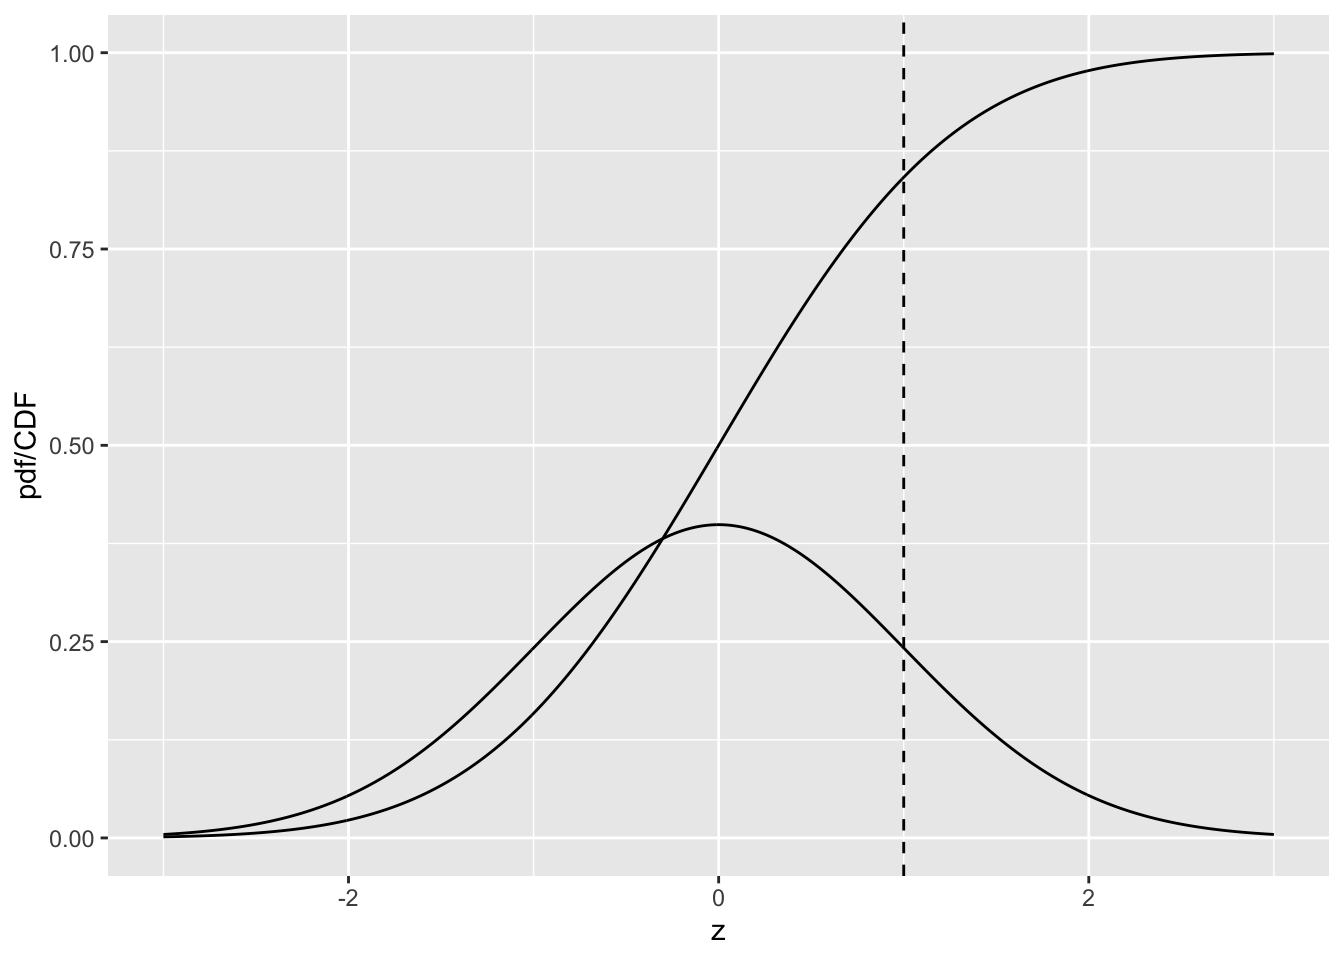
\includegraphics{03-modeling-binary-task_files/figure-latex/binary-task-model-plots1-1.pdf}
\caption{\label{fig:binary-task-model-plots1}pdf-CDF plots for the unit normal distribution. The red curve is the pdf and the blue line is the CDF. The dashed line is the reporting threshold \(\zeta = 1\).}
\end{figure}

Fig. \ref{fig:binary-task-model-plots1} shows plots, as functions of z, of the CDF and the pdf for the unit normal distribution. Since z-samples outside ±3 are unlikely, the plotted range, from -3 to +3 includes most of the distribution. The pdf is the familiar bell-shaped curve, centered at zero; the corresponding \texttt{R} function is \texttt{dnorm()} the density of the unit normal distribution. The CDF \(\Phi(z)\) increases monotonically from 0 to unity as z increases from \(-\infty\) to \(+\infty\). It is the sigmoid (S-shaped) shaped curve in Fig. \ref{fig:binary-task-model-plots1}; the corresponding \texttt{R} function is \texttt{pnorm()}. The dashed line corresponds to the reporting threshold \(\zeta = 1\). The area under the pdf to the left of \(\zeta\) equals the value of CDF at the selected \(\zeta\) (\texttt{pnorm(1)} = 0.841).

A related function is the inverse of Eqn. \eqref{eq:binary-task-model-Phi}. Suppose the left hand side of Eqn. \eqref{eq:binary-task-model-Phi} is denoted \(p\), which is a probability in the range 0 to 1.

\begin{equation} 
p \equiv \Phi\left ( z \right )=\int_{-\infty }^{z}\phi(t)dt
\label{eq:binary-task-model-Phi2}
\end{equation}

The inverse of \(\Phi(z)\) is that function which when applied to \(p\) yields the upper limit \(z\) in Eqn. \eqref{eq:binary-task-model-Phi2}, i.e.,

\begin{equation} 
\Phi^{-1}(p) = z
\label{eq:binary-task-model-PhiInvDef}
\end{equation}

Since \(p \equiv \Phi(z)\) it follows that

\begin{equation} 
\Phi(\Phi^{-1}(z))=z
\label{eq:binary-task-model-PhiInvDef2}
\end{equation}

This nicely satisfies the property of an inverse function. The inverse is known in statistical terminology as the quantile function, implemented in \texttt{R} as the \texttt{qnorm()}. Think of \texttt{pnorm()} as a probability and \texttt{qnorm()} as value on the z-axis.

To summarize the convention used in \texttt{R}, \texttt{norm} implies the unit normal distribution, \texttt{p} denotes a probability distribution function or CDF, \texttt{q} denotes a quantile function and \texttt{d} denotes a density function.

\begin{Shaded}
\begin{Highlighting}[numbers=left,,]
\FunctionTok{qnorm}\NormalTok{(}\FloatTok{0.025}\NormalTok{)}
\CommentTok{\#\textgreater{} [1] {-}1.959964}
\FunctionTok{qnorm}\NormalTok{(}\DecValTok{1}\FloatTok{{-}0.025}\NormalTok{)}
\CommentTok{\#\textgreater{} [1] 1.959964}
\FunctionTok{pnorm}\NormalTok{(}\FunctionTok{qnorm}\NormalTok{(}\FloatTok{0.025}\NormalTok{))}
\CommentTok{\#\textgreater{} [1] 0.025}
\FunctionTok{qnorm}\NormalTok{(}\FunctionTok{pnorm}\NormalTok{(}\SpecialCharTok{{-}}\FloatTok{1.96}\NormalTok{))}
\CommentTok{\#\textgreater{} [1] {-}1.96}
\end{Highlighting}
\end{Shaded}

Line 1 demonstrates the identity:

\begin{equation} 
\Phi^{-1}(0.025)=-1.959964
\label{eq:binary-task-model-Phi-Inv-alpha-by2}
\end{equation}

Line 3 demonstrates the identity:

\begin{equation} 
\Phi^{-1}(1-0.025)=+1.959964
\label{eq:binary-task-model-phi-inv-alpha}
\end{equation}

Lines 5 and 7 demonstrate that \texttt{pnorm} and \texttt{qnorm}, applied in either order, are inverses of each other.

Eqn. \eqref{eq:binary-task-model-Phi-Inv-alpha-by2} means that the (rounded) value -1.96 is such that the area under the pdf to the left of this value is 0.025. Similarly, Eqn. \eqref{eq:binary-task-model-phi-inv-alpha} means that the (rounded) value +1.96 is such that the area under the pdf to the left of this value is 1-0.025 = 0.975. In other words, -1.96 captures, to its left, the 2.5th percentile of the unit-normal distribution, and 1.96 captures, to its left, the 97.5th percentile of the unit-normal distribution, Fig. \ref{fig:binary-task-model-shaded-tails}. Since between them they capture 95 percent of the unit-normal pdf, these two values can be used to estimate 95 percent confidence intervals.

\begin{figure}
\centering
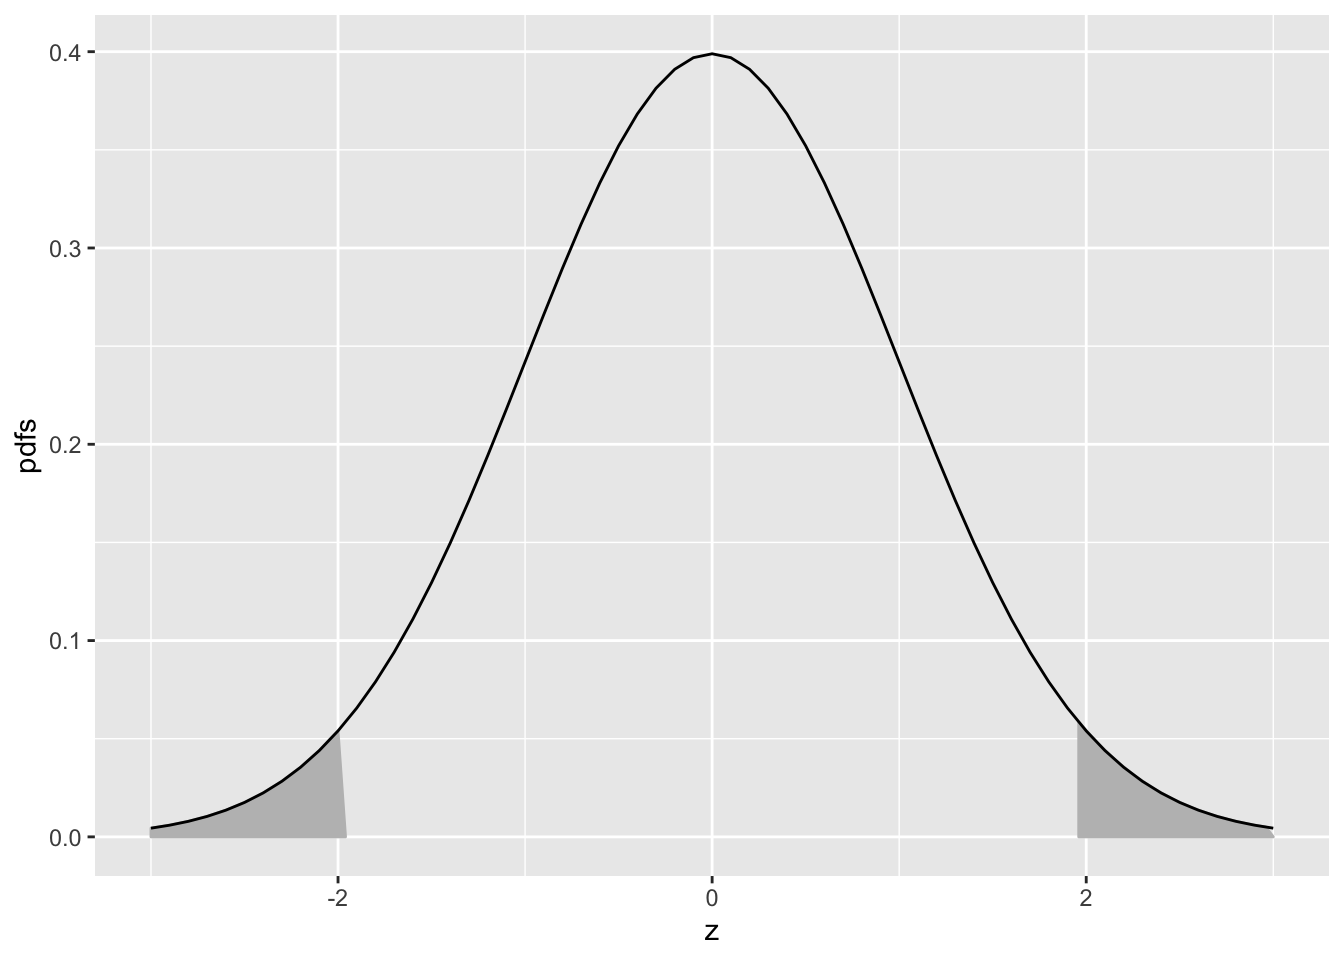
\includegraphics{03-modeling-binary-task_files/figure-latex/binary-task-model-shaded-tails-1.pdf}
\caption{\label{fig:binary-task-model-shaded-tails}Illustrating that 95 percent of the total area under the unit normal pdf is contained in the range \textbar Z\textbar{} \textless{} 1.96, which can be used to construct a 95 percent confidence interval for an estimate of a suitably normalized statistic. The area in each shaded tail is 0.025.}
\end{figure}

\begin{quote}
If one knows that a variable is distributed as a unit-normal random variable, then the observed value minus 1.96 defines the lower limit of its 95 percent confidence interval, and the observed value plus 1.96 defines the upper limit of its 95 percent confidence interval.
\end{quote}

\hypertarget{binary-task-model-sensitivity-specificity}{%
\section{Analytic expressions for specificity and sensitivity}\label{binary-task-model-sensitivity-specificity}}

Specificity corresponding to threshold \(\zeta\) is the probability that a Z-sample from a non-diseased case is smaller than \(\zeta\). By definition, this is the CDF corresponding to the threshold \(\zeta\). In other words:

\begin{equation} 
\left.
\begin{aligned}  
Sp\left ( \zeta \right ) \equiv& P\left ( Z_{k_11} < \zeta\mid Z_{k_11} \sim N\left ( 0,1 \right )\right ) \\
=& \Phi\left ( \zeta \right )
\end{aligned}
\right \}
\label{eq:binary-task-model-specificity}
\end{equation}

The expression for sensitivity can be derived. Consider that the random variable obtaining by shifting the origin to \(\mu\). A little thought should convince the reader that \(Z_{k_22}-\mu\) is distributed as \(N(0,1)\). Therefore, the desired probability is:

\begin{equation} 
\left.
\begin{aligned}  
Se\left ( \zeta \right ) \equiv& P\left ( Z_{k_22} \geq \zeta\right ) \\
=&P\left (\left ( Z_{k_22} -\mu  \right ) \geq\left ( \zeta -\mu  \right )\right ) \\
=&1-P\left (\left ( Z_{k_22} -\mu  \right ) < \left ( \zeta -\mu  \right )\right ) \\
=& 1-\Phi\left ( \zeta -\mu \right )
\end{aligned}
\right \}
\label{eq:binary-task-model-sensitivity}
\end{equation}

A little thought, based on the definition of the CDF function and the symmetry of the unit-normal pdf function, should convince the reader that:

\begin{equation} 
\left.
\begin{aligned}  
1-\Phi(\zeta)=& -\Phi(\zeta)\\
1-\Phi(\zeta-\mu) =& \Phi(\mu-\zeta)
\end{aligned}
\right \}
\label{eq:binary-task-model-compact}
\end{equation}

Instead of carrying the ``1 minus'' around one can use the more compact notation. Summarizing, the analytical formulae for the specificity and sensitivity for the equal-variance binormal model are:

\begin{equation} 
Sp\left ( \zeta \right ) = \Phi(\zeta)\\
Se\left ( \zeta \right ) = \Phi(\mu-\zeta)
\label{eq:binary-task-model-se-sp}
\end{equation}

\begin{quote}
In Eqn. \eqref{eq:binary-task-model-se-sp} the threshold \(\zeta\) appears with different signs because specificity is the area under a pdf to the left of the threshold while sensitivity is the area to the right.
\end{quote}

Sensitivity and specificity are restricted to the range 0 to 1. The observer's performance could be characterized by specifying sensitivity \emph{and} specificity, i.e., a pair of numbers. If both sensitivity and specificity of an imaging system are greater than the corresponding values for another system, then the first system is unambiguously better than the second. But if sensitivity is greater for the first but specificity is greater for the second the comparison is ambiguous. A scalar measure is desirable that combines sensitivity and specificity into a single measure of diagnostic performance.

The parameter \(\mu\) satisfies the requirements of a scalar performancer measure, termed a figure of merit (FOM). Eqn. \eqref{eq:binary-task-model-se-sp} can be solved for \(\mu\) as follows. Inverting the equations yields:

\begin{equation} 
\left.
\begin{aligned}  
\zeta =&\Phi^{-1} \left (\text{Sp}\left ( \zeta \right )  \right )\\
\mu - \zeta =& \Phi^{-1} \left (\text{Se}\left ( \zeta \right )  \right )
\end{aligned}
\right \}
\label{eq:binary-task-model-solve-mu-zeta}
\end{equation}

Eliminating \(\zeta\) yields:

\begin{equation} 
\left.
\begin{aligned}  
\mu =& \Phi^{-1} \left (\text{Sp}\left ( \zeta \right )  \right ) + \Phi^{-1} \left (\text{Se}\left ( \zeta \right )  \right )
\end{aligned}
\right \}
\label{eq:binary-task-model-solve-mu}
\end{equation}

This is a useful relation, as it converts a \emph{pair} of numbers into a \emph{scalar} performance measure. Now it is almost trivial to compare two modalities: the one with the higher \(\mu\) is better. In reality, the comparison is not trivial since like sensitivity and specificity \(\mu\) has to be estimated from a finite dataset and one must account for sampling variability.

\begin{figure}
\centering
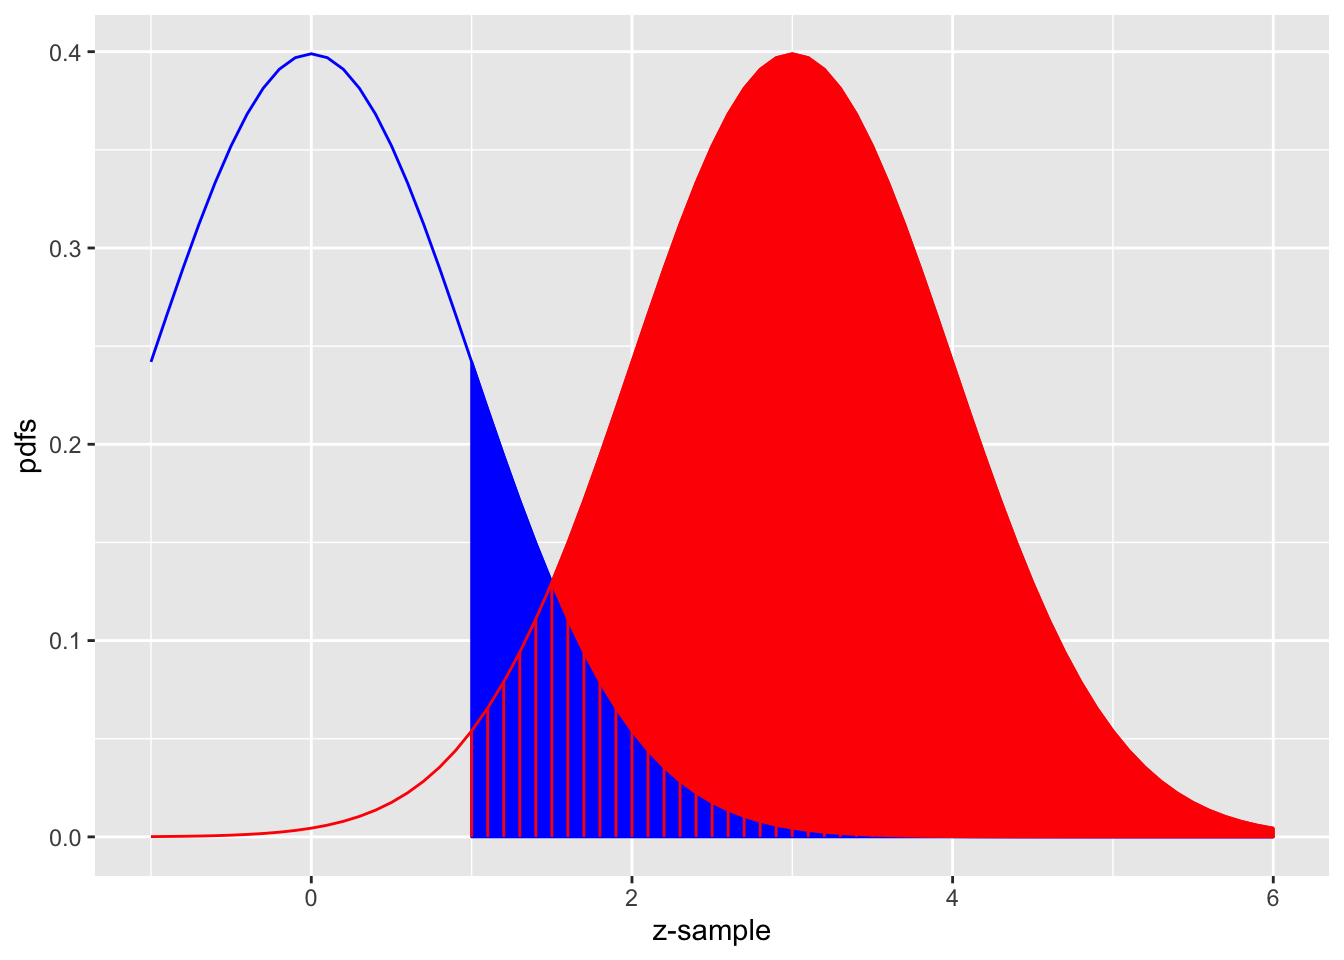
\includegraphics{03-modeling-binary-task_files/figure-latex/binary-task-model-shaded-plots-1.pdf}
\caption{\label{fig:binary-task-model-shaded-plots}The equal-variance binormal model for \(\mu = 3\) and \(\zeta = 1\); the blue curve, centered at zero, is the pdf of non-diseased cases and the red one, centered at \(\mu = 3\), is the pdf of diseased cases. The left edge of the blue shaded region represents the threshold \(\zeta = 1\). The red shaded area including the common portion with the vertical red lines is sensitivity. The blue shaded area including the common portion with the vertical red lines is 1-specificity.}
\end{figure}

Fig. \ref{fig:binary-task-model-shaded-plots} shows the equal-variance binormal model for \(\mu = 3\) and \(\zeta = 1\). The blue-shaded area, including the ``common'' portion with the vertical red lines, is the probability that a z-sample from a non-diseased case exceeds \(\zeta = 1\), which is the complement of specificity, i.e., false positive fraction, which is 1 - \texttt{pnorm(1)} = 0.159. The red shaded area, including the ``common'' portion with the vertical red lines, is the probability that a z-sample from a diseased case exceeds \(\zeta = 1\), which is sensitivity or true positive fraction, which is \texttt{pnorm(3-1)}= 0.977.

See Appendix \ref{binary-task-model-demo} for a demonstration of the concepts of sensitivity and specificity using \texttt{R}.

\hypertarget{binary-task-model-sensitivity-specificity-inverse-variation}{%
\section{Inverse variation of sensitivity and specificity}\label{binary-task-model-sensitivity-specificity-inverse-variation}}

The variation of sensitivity and specificity is modeled in the binormal model by the threshold parameter \(\zeta\). From Eqn. \eqref{eq:binary-task-model-specificity} specificity at threshold \(\zeta\) is \(\text{Sp} = \Phi(\zeta)\) and sensitivity is \(\text{Se} = \Phi(\mu-\zeta)\). Since the threshold \(\zeta\) appears with different signs the dependence of sensitivity on \(\zeta\) will be the opposite of that of specificity. In Fig. \ref{fig:binary-task-model-shaded-plots}, the left edge of the blue shaded region represents the threshold \(\zeta = 1\). As \(\zeta = 1\) is moved towards the left, specificity decreases but sensitivity increases. Specificity decreases because less of the non-diseased distribution lies to the left of the lowered threshold, in other words fewer non-diseased cases are correctly diagnosed as non-diseased. Sensitivity increases because more of the diseased distribution lies to the right of the lowered threshold, in other words more diseased cases are correctly diagnosed as diseased.

If Observer 1 has higher sensitivity than Observer 2 but lower specificity it is difficult to unambiguously compare them; it is not impossible \citep{RN2637}. The unambiguous comparison is difficult for the following reason: assuming the Observer 2 can be coaxed into adopting a lower threshold, thereby decreasing specificity to match that of Observer 1 then it is possible that the Observer 2's sensitivity, formerly smaller, could (and here is the ambiguity because if might not happen) now be greater than that of Observer 1.

A single figure of merit is desirable to the sensitivity - specificity analysis. It is possible to leverage the inverse variation of sensitivity and specificity by combing them into a single scalar measure, as was done with the \(\mu\) parameter in the previous section, Eqn. \eqref{eq:binary-task-model-solve-mu}.

An equivalent way is by using the area under the ROC plot, discussed next.

\hypertarget{binary-task-model-roc-curve}{%
\section{The ROC curve}\label{binary-task-model-roc-curve}}

The receiver operating characteristic (ROC) is defined as the plot of sensitivity (y-axis) vs.~1-specificity (x-axis). Equivalently, it is the plot of TPF (y-axis) vs.~FPF (x-axis). From Eqn. \eqref{eq:binary-task-model-se-sp} it follows that:

\begin{equation} 
\left.
\begin{aligned}  
\text{FPF}\left ( \zeta \right ) &\equiv 1 - \text{Sp}\left ( \zeta \right ) \\
&=\Phi\left ( -\zeta \right )\\
\text{TPF}\left ( \zeta \right ) &\equiv \text{Se}\left ( \zeta \right ) \\
&=\Phi\left (\mu -\zeta \right )\\ 
\end{aligned}
\right \}
\label{eq:binary-task-model-fpf-tpf}
\end{equation}

Specifying \(\zeta\) selects a particular operating point on this curve and varying \(\zeta\) from \(+\infty\) to \(-\infty\) causes the operating point to trace out the ROC curve from the origin (0,0) to (1,1). Note that as \(\zeta\) increases the operating point moves down the curve. The operating point \(O(\zeta|\mu)\) for the equal variance binormal model is:

\begin{equation} 
O\left ( \zeta \mid \mu \right ) = \left ( \Phi(-\zeta), \Phi(\mu-\zeta) \right ) \\
\label{eq:binary-task-model-op-pt}
\end{equation}

The operating point predicted by the above equation lies exactly on the theoretical ROC curve. This condition can only be achieved with very large numbers of cases. With finite datasets the operating point will almost never be exactly on the theoretical curve.

\begin{quote}
The ROC curve is the locus of the operating point for fixed \(\mu\) and variable \(\zeta\). Fig. \ref{fig:binary-task-model-rocs} shows examples of equal-variance binormal model ROC curves for different values of \(\mu\). Each has the property that TPF is a monotonically increasing function of FPF and the slope decreases monotonically as the operating point moves up the curve. As \(\mu\) increases the curves get progressively upward-left shifted, approaching the top-left corner of the ROC plot. In the limit \(\mu = \infty\) the curve degenerates into two line segments, a vertical one connecting the origin to (0,1) and a horizontal one connecting (0,1) to (1,1) -- the ROC plot for a perfect observer.
\end{quote}

\begin{figure}
\centering
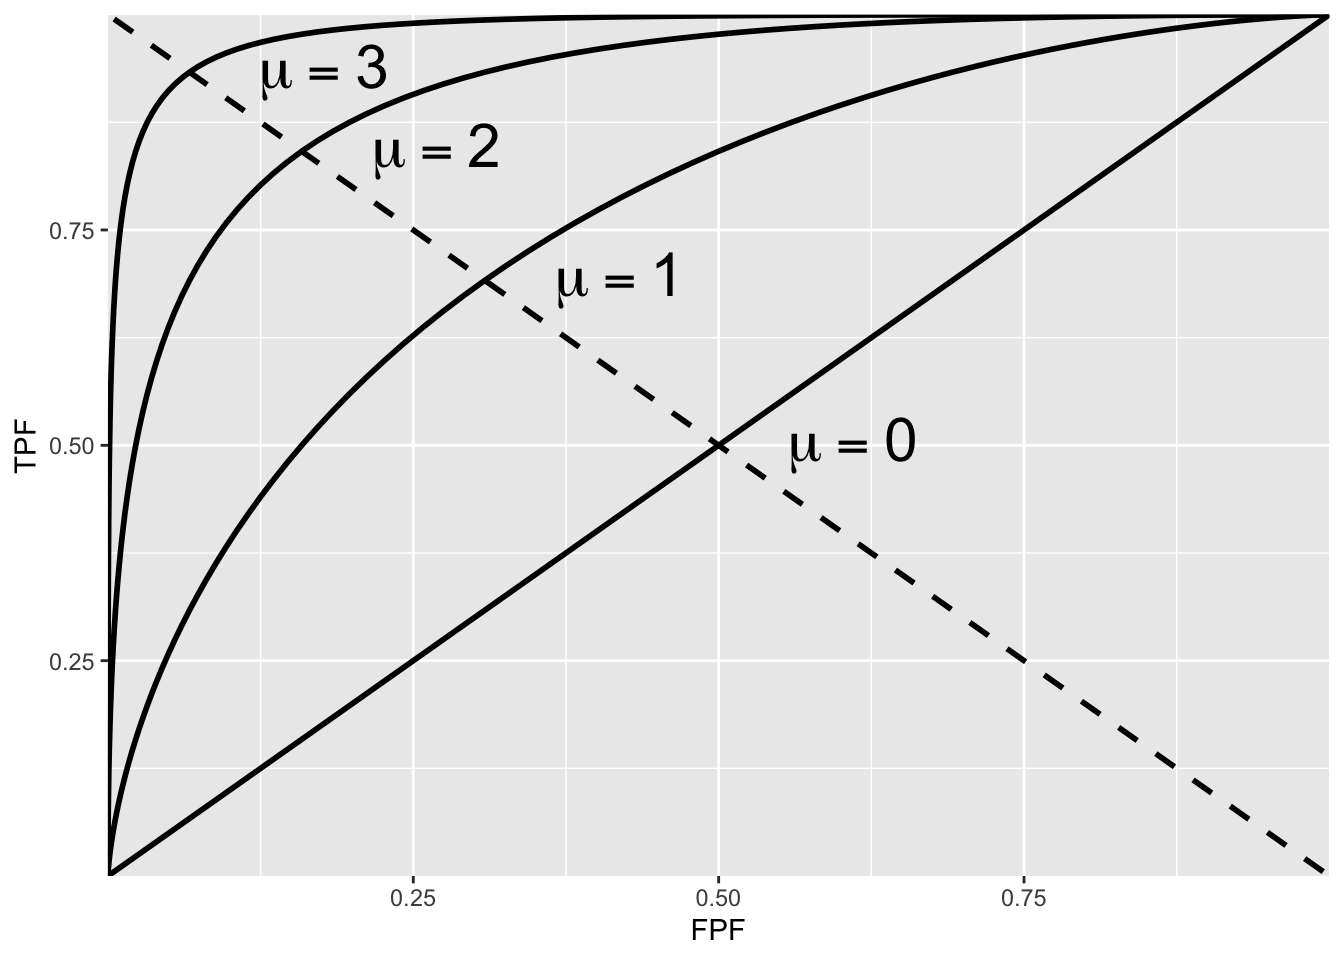
\includegraphics{03-modeling-binary-task_files/figure-latex/binary-task-model-rocs-1.pdf}
\caption{\label{fig:binary-task-model-rocs}ROC plots predicted by the equal variance binormal model for different values of \(\mu\). As \(\mu\) increases the intersection of the curve with the negative diagonal moves closer to the ideal operating point, (0,1) at which sensitivity and specificity are both equal to unity.}
\end{figure}

\hypertarget{binary-task-model-chance-diagonal}{%
\subsection{The chance diagonal}\label{binary-task-model-chance-diagonal}}

In Fig. \ref{fig:binary-task-model-rocs} the ROC curve for \(\mu=0\) is the positive diagonal of the ROC plot, termed the \textbf{chance diagonal}. Along this curve \(\text{TPF = FPF}\) and the observer's performance is at chance level. For \(\mu=0\) the pdf of the diseased distribution is identical to that of the non-diseased distribution: both are centered at the origin. Therefore, no matter the choice of threshold \(\zeta\), \(\text{TPF = FPF}\). Setting \(\mu=0\) in Eqn. \eqref{eq:binary-task-model-fpf-tpf} yields:

\[\text{TPF}\left ( \zeta \right )=\text{FPF}\left ( \zeta \right )=\Phi\left ( -\zeta \right )\]
In this case the red and blue curves in Fig. \ref{fig:binary-task-model-shaded-plots} coincide. The observer is unable to find any difference between the two distributions. This can happen if the cancers are of such low visibility that diseased cases are indistinguishable from non-diseased ones, or the observer's skill level is so poor that the observer is unable to make use of distinguishing characteristics between diseased and non-diseased cases that do exist and which experts exploit.

\hypertarget{binary-task-model-guessing-observer}{%
\subsection{The guessing observer}\label{binary-task-model-guessing-observer}}

If the cases are indeed impossibly difficult and/or the observer has zero skill at discriminating between them, the observer has no option but to guess. This rarely happens in the clinic, as too much is at stake and this paragraph is intended to make a pedagogical point: the observer can move the operating point along the change diagonal. If there is no special incentive, the observer tosses a coin and if the coin lands head up, the observer states: ``case is diseased'' and otherwise states: ``case is non-diseased''. When this procedure is averaged over many non-diseased and diseased cases, it will result in the operating point (0.5, 0.5). \footnote{Many cases are assumed as otherwise, due to sampling variability, the operating point will not be on the theoretical ROC curve.} To move the operating point downward, e.g., to (0.1, 0.1) the observer randomly selects an integer number between 1 and 10, equivalent to a 10-sided ``coin''. Whenever a one ``shows up'', the observer states ``case is diseased'' and otherwise the observer states ``case is non-diseased''. To move the operating point to (0.2, 0.2) whenever a one or two ``shows up'', the observer states ``case is diseased'' and otherwise the observer states ``case is non-diseased''. One can appreciate that simply by changing the probability of stating ``case is diseased'' the observer can place the operating point anywhere on the chance diagonal but wherever the operating point is placed, it will satisfy TPF = FPF.

\hypertarget{binary-task-model-symmetry-wrt-negative-diagonal}{%
\subsection{Symmetry with respect to negative diagonal}\label{binary-task-model-symmetry-wrt-negative-diagonal}}

A characteristic of the ROC curves shown in Fig. \ref{fig:binary-task-model-rocs} is that they are symmetric with respect to the negative diagonal, i.e., the line joining (0,1) and (1,0) which is shown as the dotted straight line in Fig. \ref{fig:binary-task-model-rocs}. The symmetry property is due to the equal variance nature of the binormal model and is not true for models considered in later chapters. The intersection between the ROC curve and the negative diagonal corresponds to \(\zeta = \mu/2\), in which case the operating point is:

\begin{equation} 
\left.
\begin{aligned}  
\text{FPF}\left ( \zeta \right ) &=\Phi\left ( -\mu/2 \right )\\
\text{TPF}\left ( \zeta \right ) &=\Phi\left (\mu/2 \right )\\ 
\end{aligned}
\right \}
\label{eq:binary-task-model-neg-diag}
\end{equation}

The first equation implies:

\[1-\text{FPF}\left ( \zeta \right ) =1-\Phi\left ( -\mu/2 \right )= \Phi\left ( \mu/2 \right )\]

Therefore,

\begin{equation} 
\text{TPF}\left ( \zeta \right ) = 1-\text{FPF}\left ( \zeta \right )
\label{eq:binary-task-model-neg-diag2}
\end{equation}

This equation describes a straight line with unit intercept and slope equal to minus 1, which is the negative diagonal. Since \(\text{TPF = Se}\) and \(\text{FPF = 1-Sp}\) another way of stating this is that at the intersection with the negative diagonal sensitivity equals specificity.

\hypertarget{binary-task-model-auc-roc-important}{%
\subsection{Area under the ROC curve}\label{binary-task-model-auc-roc-important}}

\begin{quote}
The area AUC (abbreviation for area under curve) under the ROC curve suggests itself as a measure of performance that is independent of threshold and therefore circumvents the ambiguity issue of comparing sensitivity/specificity pairs, and has other advantages.
\end{quote}

It is defined by the following integrals:

\begin{equation} 
\begin{aligned}
A_{z;\sigma = 1} &= \int_{0}^{1}TPF(\zeta)d(FPF(\zeta))\\
&=\int_{0}^{1}FPF(\zeta)d(TPF(\zeta))\\
\end{aligned}
\label{eq:binary-task-model-az-eq-var}
\end{equation}

Eqn. \eqref{eq:binary-task-model-az-eq-var} has the following equivalent interpretations:

\begin{itemize}
\item
  The first form performs the integration using thin vertical strips, e.g., extending from x to x + dx, where x is a temporary symbol for FPF. The area can be interpreted as the average TPF over all possible values of FPF.
\item
  The second form performs the integration using thin horizontal strips, e.g., extending from y to y + dy, where y is a temporary symbol for TPF. The area can be interpreted as the average FPF over all possible values of TPF.
\end{itemize}

By convention, the symbol \(A_z\) is used for the area under the unequal-variance binormal model predicted ROC curve. The more expressive term area under curve or AUC is used to include this and other methods of estimating the area under the ROC curve.

In Eqn. \eqref{eq:binary-task-model-az-eq-var}, the extra subscript \(\sigma = 1\) is necessary to distinguish it from another that corresponding to the unequal variance binormal model to be derived later. It can be shown that:

\begin{equation} 
A_{z;\sigma = 1} = \Phi\left ( \frac{\mu} {\sqrt{2}} \right )
\label{eq:binary-task-model-az-var}
\end{equation}

Since the ROC curve is bounded by the unit square, \(A_z\) must be between zero and one. If \(\mu\) is non-negative, \(A_{z;\sigma = 1}\) must be between 0.5 and 1. The chance diagonal, corresponding to \(\mu = 0\), yields \(A_{z;\sigma = 1} = 0.5\), while the perfect ROC curve, corresponding to \(\mu = \infty\) yields \(A_{z;\sigma = 1} = 1\).

\begin{quote}
Since it is a scalar quantity, \(A_z\) can be used to unambiguously quantify performance than is possible using sensitivity - specificity pairs.
\end{quote}

\hypertarget{binary-task-model-properties-roc}{%
\subsection{Properties of the equal-variance binormal model ROC curve}\label{binary-task-model-properties-roc}}

\begin{enumerate}
\def\labelenumi{\arabic{enumi}.}
\item
  The ROC curve is completely contained within the unit square. This follows from the fact that both axes of the plot are probabilities.
\item
  The operating point rises monotonically from (0,0) to (1,1).
\item
  Since \(\mu\) is positive, the slope of the equal-variance binormal model curve at the origin (0,0) is infinite and the slope at (1,1) is zero, and the slope along the curve is always non-negative and decreases monotonically as the operating point moves up the curve.
\item
  \(A_z\) is a monotone increasing function of \(\mu\). It varies from 0.5 to 1 as \(\mu\) varies from zero to infinity.
\end{enumerate}

\hypertarget{binary-task-model-comments}{%
\subsection{Comments}\label{binary-task-model-comments}}

Property 2: since the operating point can both be expressed in terms of \(\Phi\) functions, which are monotone in their arguments, and in each case the argument \(\zeta\) appears with a negative sign it follows that as \(\zeta\) is lowered both TPF and FPF increase. The operating point corresponding to \(\zeta - d\zeta\) is to the upper right of that corresponding \(\zeta\) to (assuming \(d\zeta > 0\)).

Property 3: The slope of the ROC curve can be derived by differentiation (\(\mu\) is constant):

\begin{equation} 
\left.
\begin{aligned}
\frac{d(TPF)}{d(FPF)}&=\frac{d(\Phi(\mu-\zeta))}{d(\Phi(-\zeta))}\\
&=\frac{\phi(\mu-\zeta)}{\phi(-\zeta)}\\
&=\exp(\mu(\zeta-\mu/2)) \propto \exp(\mu \zeta)\\
\end{aligned}
\right \}
\label{eq:binary-task-model-slope1}
\end{equation}

The above derivation uses the fact that the differential of the CDF function yields the pdf function, i.e.,

\[d\Phi(\zeta)=P\left ( \zeta < Z < \zeta + d \zeta \right ) = \phi(\zeta)d\zeta\]

Since the slope of the ROC curve can be expressed as a power of \(e\) it is always non-negative. Provided \(\mu > 0\), in the limit \(\zeta\rightarrow \infty\) the slope at the origin approaches \(\infty\). Eqn. \eqref{eq:binary-task-model-slope1} also implies that in the limit \(\zeta\rightarrow -\infty\) the slope of the ROC curve at the end-point (1,1) approaches zero, i.e., the slope is a monotone increasing function of \(\zeta\). As \(\zeta\) decrease from \(+\infty\) to \(-\infty\), the slope decreases monotonically from \(+\infty\) to 0.

Fig. \ref{fig:binary-task-model-analytical-roc} is the ROC curve for the equal-variance binormal model for \(\mu = 3\). The entire curve is defined by varying \(\zeta\). Specifying a particular value of \(\zeta\) corresponds to specifying a particular point on the ROC curve. In Fig. TBA 3.5 the open circle corresponds to the operating point (0.159, 0.977) defined by \(\zeta = 1\): \texttt{pnorm(-1)} = 0.159; pnorm(3-1) = 0.977. The operating point lies exactly on the curve as this is a predicted operating point.

\begin{figure}
\centering
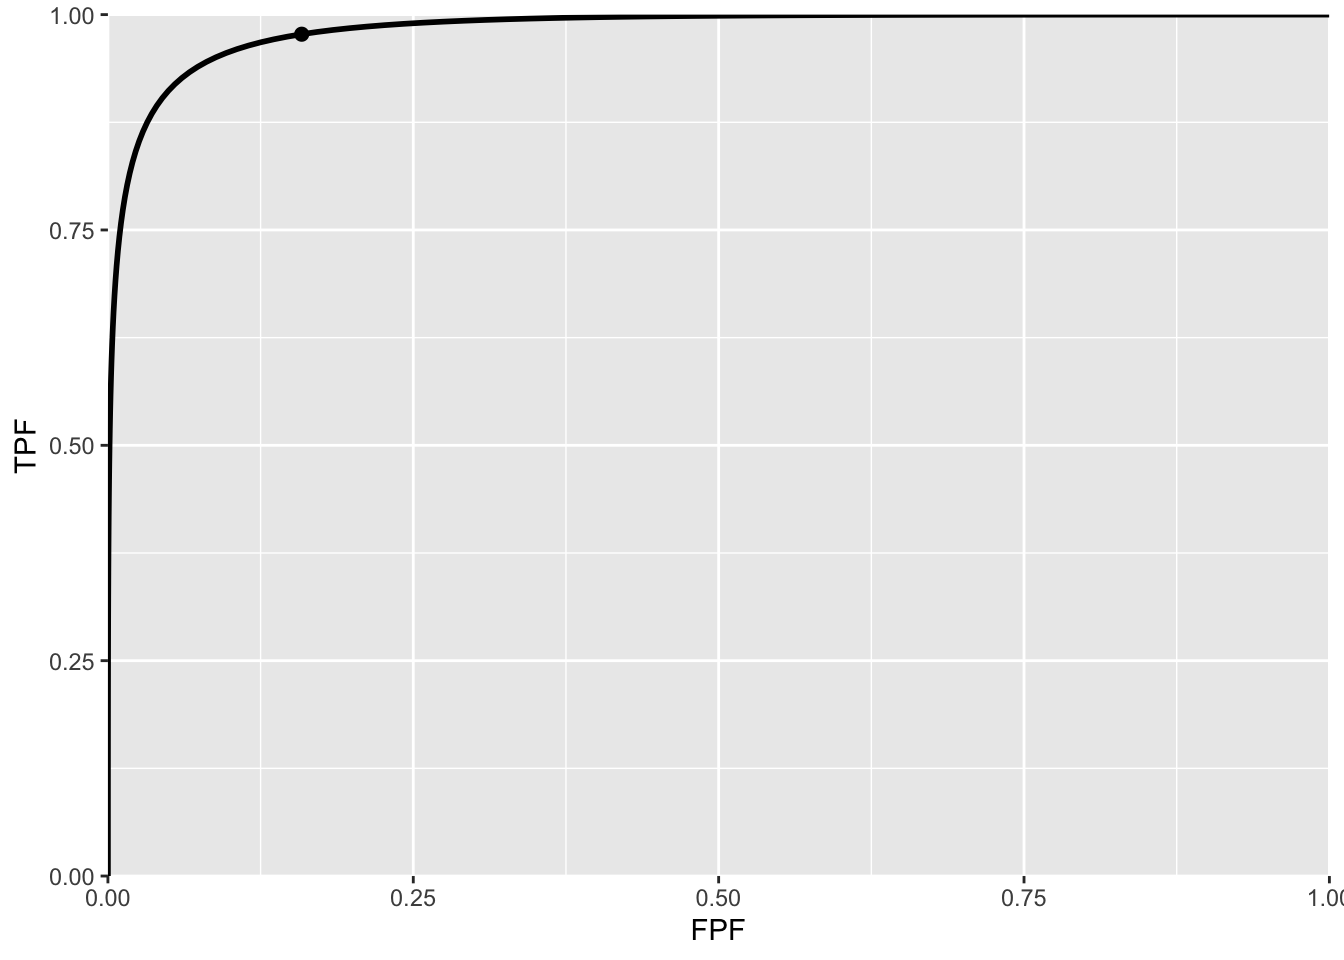
\includegraphics{03-modeling-binary-task_files/figure-latex/binary-task-model-analytical-roc-1.pdf}
\caption{\label{fig:binary-task-model-analytical-roc}ROC curve predicted by equal variance binormal model for \(\mu = 3\). The circled operating point corresponds to \(\zeta = 1\). The operating point falls exactly on the curve, as these are analytical curves. With finite numbers of cases this is not observed in practice.}
\end{figure}

\hypertarget{binary-task-model-mu-parameter-intepretation}{%
\subsection{Physical interpretation of the mu-parameter}\label{binary-task-model-mu-parameter-intepretation}}

The \(\mu\) parameter is equivalent \citep{macmillan2004detection} to a signal detection theory variable denoted \(d'\) in the literature (pronounced ``dee-prime''). It can be thought of as the \emph{perceptual signal to noise ratio} (pSNR) of diseased cases relative to non-diseased ones. It is a measure of reader expertise and / or ease of detectability of the disease. SNR is a term widely used in engineering, specifically in signal detection theory \citep{green1966signal, egan1975book}. It dates to the early 1940s when one had the problem \citep[\citet{marcum1960statistical}]{marcum1947statistical} of detecting faint radar reflections from a plane against a background of noise. The radar radio ``receiver'' is the origin of the term in Receiver Operating Characteristic.

The reader may be aware of the ``rule-of-thumb'' that if SNR exceeds three the target is likely to be detected. It will be shown later that the area under the ROC curve is the probability that a diseased case Z-sample is greater than that of a non-diseased one. The following code snippet shows that for \(\mu = 3\), the probability of detection is 98.3 percent.

\begin{verbatim}
#> pnorm(3/sqrt(2)) =  0.983
\end{verbatim}

For electrical signals, SNR can be measured with instruments but, in the context of decisions made by humans, what is measured is the \emph{perceptual} SNR. Physical characteristics that differentiate non-diseased from diseased cases, and how well they are displayed will affect it; in addition the eye-sight of the observer is an obvious factor; not so obvious is how information is processed by the cognitive system, and the role of the observer's expertise.

\begin{quote}
To this day I find it remarkable that an objective SNR-like quantity can be teased out of subjective observer decisions.
\end{quote}

\hypertarget{binary-task-model-confidence-intervals}{%
\section{Confidence intervals for an operating point}\label{binary-task-model-confidence-intervals}}

\begin{itemize}
\item
  A \((1-\alpha)\) confidence interval (CI) of a statistic is the range that is expected to contain the true value with probability \((1-\alpha)\).
\item
  It should be clear that a 99 percent CI is wider than a 95 percent CI, and that a 90 percent CI is narrower; in general, the higher the confidence that the interval contains the true value, the wider the range of the CI.
\item
  Calculation of a parametric confidence interval requires a distributional assumption (non-parametric estimation methods, which use resampling methods, are described later). With a distributional assumption the parameters of the distribution can be estimated and since the distribution accounts for variability, the needed confidence interval estimate follows.
\item
  With TPF and FPF, each of which involves a ratio of two integers, it is convenient to assume a \emph{binomial} distribution for the following reason:
\item
  The diagnosis ``non-diseased'' vs.~``diseased'' represents a Bernoulli trial, i.e., one whose outcome is binary.
\item
  A Bernoulli trial is like a coin-toss, a special coin whose probability of landing ``diseased'' face up is \(p\) which is not necessarily 0.5 as with a real coin.
\item
  It is a theorem in statistics that the total number of Bernoulli outcomes of one type, e.g., \(n(FP)\), is a binomial-distributed random variable, with success probability \(\widehat{FPF}\) and trial size \(K_1\).
\end{itemize}

\begin{equation} 
n(FP) \sim B\left ( K_1, \widehat{FPF} \right )
\label{eq:binary-task-model-BinDistrFPF}
\end{equation}

\(B(n,p)\) denotes the binomial distribution with success probability \(p\) and trial size \(n\):

\begin{equation} 
\left.
\begin{aligned}  
k \sim& B\left ( n, p \right )\\
k=& 0,1,2,...,n\\
\end{aligned}
\right \}
\label{eq:binary-task-model-bin-distr}
\end{equation}

Eqn. \eqref{eq:binary-task-model-bin-distr} states that \(k\) is a random sample from the binomial distribution \(B(n,p)\). For reference, the probability mass function \(\text{pmf}\) of \(B(n,p)\) is defined by (the subscript \(Bin\) denotes a binomial distribution):

\begin{equation} 
\text{pmf}_{Bin}\left ( k;n,p \right )=\binom{n}{k}p^k(1-p)^{n-k}
\label{eq:binary-task-model-bin-distr2}
\end{equation}

For a discrete distribution, one has probability \emph{mass} function in contrast to a continuous distribution where one has a probability \emph{density} function.

The binomial coefficient \(\binom{n}{k}\) appearing in Eqn. \eqref{eq:binary-task-model-bin-distr2}, to be read as ``\(n\) pick \(k\)'', is defined by:

\begin{equation} 
\binom{n}{k}=\frac{n!}{k!(n-k)!}
\label{eq:binary-task-model-bin-coeff}
\end{equation}

From the properties of the binomial distribution the variance of n(FP) is given by:

\begin{equation} 
\sigma_{n(FP)}^2=K_1\widehat{\text{FPF}}\left ( 1 - \widehat{\text{FPF}} \right )
\label{eq:binary-task-model-var-n-FP}
\end{equation}

It follows that \(\text{FPF}\) has mean \(\widehat{\text{FPF}}\) and variance \(\sigma_{\text{FPF}}^2\) given by (since \(Var(aX) = a^2 Var(X)\) where \(a\) is a constant):

\begin{equation} 
\sigma_{\text{FPF}}^2 = \frac{\widehat{\text{FPF}}\left ( 1 - \widehat{\text{FPF}} \right )}{K_1}
\label{eq:binary-task-model-var-fpf}
\end{equation}

For large \(K_1\) the distribution of \(\text{FPF}\) approaches a normal distribution:

\begin{equation} 
\left.
\begin{aligned}  
FPF \sim N\left ( \widehat{\text{FPF}}, \sigma_{\text{FPF}}^2 \right )\end{aligned}
\right \}
\label{eq:binary-task-model-distr-fpf}
\end{equation}

Eqn. \eqref{eq:binary-task-model-distr-fpf} allows us to write down the approximate symmetric confidence interval for \(\widehat{\text{FPF}}\), i.e., \(\pm z_{\alpha/2} \times \sigma_{\text{FPF}}\) around \(\widehat{\text{FPF}}\).

\begin{equation} 
CI_{1-\alpha}^{\text{FPF}}=\left ( \widehat{\text{FPF}} - z_{\alpha/2} \sigma_{\text{FPF}}, \widehat{\text{FPF}} + z_{\alpha/2} \sigma_{\text{FPF}} \right )
\label{eq:binary-task-model-ci-fpf}
\end{equation}

In Eqn. \eqref{eq:binary-task-model-ci-fpf} \(z_{\alpha/2}\) is the upper \(\alpha/2\) quantile of the unit normal distribution: it is defined such that the area to the \emph{right} under the unit normal distribution pdf from \(z_{\alpha/2}\) to \(+\infty\) equals \(\alpha/2\). For example \(z_{0.025} = 1.96\), see Fig. \ref{fig:binary-task-model-shaded-tails}. In general \(z_{\alpha/2} = -\Phi^{-1}(\alpha/2)\). For example \texttt{-qnorm(0.025)} = 1.96.

These relations involving \(z_{\alpha/2}\) follow:

\begin{equation} 
\left.
\begin{aligned} 
z_{\alpha/2} &=\Phi^{-1}\left ( 1-\alpha/2 \right )\\
&= - \Phi^{-1}\left (\alpha/2 \right )\\
\alpha/2&=\int_{z_{\alpha/2}}^{\infty}\phi(z)dz\\ 
&= 1-\Phi(z_{\alpha/2})\\
&= \Phi(-z_{\alpha/2})\\
\end{aligned}
\right \} 
\label{eq:binary-task-model-def-z-alpha2}
\end{equation}

The normal approximation is adequate if both of the following two conditions are both met: \(K_1\widehat{FPF} > 10\) and \(K_1(1-\widehat{\text{FPF}}) > 10\). This means, approximately, that \(\widehat{\text{FPF}}\) cannot be too close to zero or 1.

Similarly, an approximate symmetric \((1-\alpha)\) confidence interval for \(\text{TPF}\) is:

\begin{equation} 
CI_{1-\alpha}^{\text{TPF}}=\left ( \widehat{\text{TPF}} - z_{\alpha/2} \sigma_{\text{TPF}}, \widehat{\text{TPF}} + z_{\alpha/2} \sigma_{\text{TPF}} \right )
\label{eq:binary-task-model-ci-tpf}
\end{equation}

In Eqn. \eqref{eq:binary-task-model-ci-tpf},

\begin{equation} 
\sigma_{\text{TPF}}^2 = \frac{\widehat{\text{TPF}}\left ( 1 - \widehat{\text{TPF}} \right )}{K_2}
\label{eq:binary-task-model-var-tpf}
\end{equation}

The confidence intervals are largest when the probabilities (FPF or TPF) are close to 0.5 and decrease inversely as the square root of the relevant number of cases. The symmetric binomial distribution based estimates can stray outside the allowed range (0 to 1). Exact confidence intervals that are asymmetric around the central value and which are guaranteed to be in the allowed range can be calculated: it is implemented in \texttt{R} in function \texttt{binom.test()}and used below:

\begin{verbatim}
#> alpha =  0.05 
#> K1 =  99 
#> K2 =  111 
#> mu =  5 
#> zeta =  2.5
#> Specificity =  0.99 
#> Sensitivity =  0.991
#> Approx 95 percent CI for Specificity =  0.97 1.01
#> Exact 95 percent CI for Specificity =  0.945 1
#> Approx 95 percent CI for Sensitivity =  0.973 1.01
#> Exact 95 percent CI for Sensitivity =  0.951 1
\end{verbatim}

Note that the approximate confidence intervals can stray outside the allowed range but the exact confidence intervals do not.

\hypertarget{binary-task-model-beam-study}{%
\section{Variability: the Beam study}\label{binary-task-model-beam-study}}

In this study \citep{beam1996variability} fifty accredited mammography centers were randomly sampled in the United States. ``Accredited'' is a legal/regulatory term implying, among other things, that the radiologists interpreting the breast cases were ``board certified'' by the American Board of Radiology. One hundred eight (108) certified radiologists from these centers gave blinded interpretation to a common set of 79 randomly sampled (stratified sampling) enriched screening cases containing 45 cases with cancer and the rest with benign lesions. Ground truth for these women had been established either by biopsy or by 2-year follow-up.

The observed range of sensitivity (TPF) was 53 percent and the range of FPF was 63 percent; the corresponding range for the AUC was 21 percent, Table \ref{tab:binary-task-model-table-beam-study}. Empirical AUC was estimated using a 5-point BIRADS ratings of the images (the zero category was not allowed). Explanation of empirical AUC is deferred to Chapter \ref{empirical-auc}.

\begin{table}

\caption{\label{tab:binary-task-model-table-beam-study}The variability of 108 radiologists on a common dataset of screening mammograms. Note the reduced variability when one uses AUC which accounts for variations in reporting thresholds (AUC variability range is 21 percent compared to 53 percent for sensitivity and 63 percent for specificity).}
\centering
\begin{tabular}[t]{l|r|r|r}
\hline
  & Min & Max & Range\\
\hline
Sensitivity & 46.70 & 100.00 & 53.30\\
\hline
Specificity & 36.30 & 99.30 & 63.00\\
\hline
AUC & 0.74 & 0.95 & 0.21\\
\hline
\end{tabular}
\end{table}

\begin{figure}
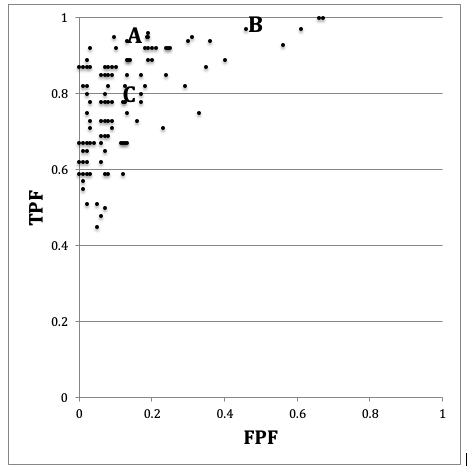
\includegraphics[width=0.8\linewidth]{images/BeamStudy} \caption{Schematic patterned from the Beam et al study showing the ROC operating points of 108 mammographers. Wide variability in sensitivity and specificity are evident while AUC is less variable. See text below.}\label{fig:beam-study-fig}
\end{figure}

In Fig. \ref{fig:beam-study-fig} if one looks at the points labeled (B) and (C) one can mentally construct a smooth ROC curve that starts at (0,0), passes roughly through these points and ends at (1,1). In this sense, the intrinsic performances (i.e., AUCs or equivalently the \(\mu\) parameters) of radiologists B and C are similar. The only difference between them is that radiologist B is using lower threshold than radiologist C. Radiologist C is more concerned with minimizing FPs while radiologist B is more concerned with maximizing sensitivity. By appropriate feedback radiologist C can perhaps be induced to change the threshold to that of radiologist B. An example of feedback might be: ``you are missing too many cancers and this could get us all into trouble; worry less about reduced specificity and more about increasing your sensitivity''.

In contrast, radiologist A has intrinsically superior performance to B or C. No change in threshold is going to get the other two to a similar level of performance as radiologist A. Extensive training will be needed to bring the under-performing radiologists to the expert level of radiologist A.

Fig. \ref{fig:beam-study-fig} and Table \ref{tab:binary-task-model-table-beam-study} illustrate several important principles.

\begin{enumerate}
\def\labelenumi{\arabic{enumi}.}
\item
  Since an operating point is characterized by two values, unless both numbers are higher (e.g., radiologist A vs.~B or C) it is difficult to unambiguously compare them.
\item
  While sensitivity and specificity depend on the reporting threshold, the area under the ROC plot is independent of it. Using the area under the ROC curve one can unambiguously compare two readers.
\item
  Combining sensitivity and the complement of specificity into a single AUC measure yields the additional benefit of lower variability. In Fig. \ref{fig:beam-study-fig}, the range for sensitivity is 53 percent while that for specificity is 63 percent. In contrast, the range for AUC is only 21 percent. This means that much of the observed variations in sensitivity and specificity are due to variations in thresholds, and using AUC eliminates this source of variability. Decreased variability of a measure is a highly desirable characteristic as it implies the measurement is more precise making it easier to detect differences between readers.
\end{enumerate}

\hypertarget{binary-task-model-discussion}{%
\section{Discussion}\label{binary-task-model-discussion}}

Sensitivity and specificity are widely used in the medical imaging literature. It is important to realize that they do not provide a complete picture of diagnostic performance, since they represent performance at a particular observer-dependent threshold. As demonstrated in Fig. \ref{fig:beam-study-fig} expert observers can and do operate at different thresholds. If using sensitivity and specificity the dependence on reporting threshold often makes it difficult to unambiguously compare observers. An additional source of variability is introduced by the varying thresholds.

The ROC curve and AUC are completely defined by the \(\mu\) parameter of the equal variance binormal model. Since both are independent of reporting threshold they overcome the ambiguity inherent in comparing sensitivity/specificity pairs. AUC is widely used in assessing imaging systems.

\begin{quote}
It should impress the reader that a subjective internal sensory perception of disease presence and an equally subjective internal threshold can be translated into an objective performance measure, such as the area under an ROC curve or equivalently, the \(\mu\) parameter. The latter has the physical meaning of a perceptual signal to noise ratio.
\end{quote}

The properties of the unit normal distribution and the binomial distribution were used to derive parametric confidence intervals for sensitivity and specificity. These were compared to exact confidence intervals. An important study was reviewed showing wide variability in sensitivity and specificity for radiologists interpreting a common set of cases in screening mammography, but smaller variability in AUCs. This is because much of the variability in sensitivity and specificity is due to variation of the reporting threshold, which does not affect the area under the ROC curve. This is an important reason for preferring comparisons based on area under the ROC curve to those based on comparing sensitivity/specificity pairs.

\hypertarget{binary-task-model-demo}{%
\section{Appendix I}\label{binary-task-model-demo}}

\hypertarget{estimates-from-a-finite-sample}{%
\subsection{Estimates from a finite sample}\label{estimates-from-a-finite-sample}}

The following embedded code simulates 9 non-diseased and 11 diseased cases. The \(\mu\) parameter is 1.5 and \(\zeta\) is \(\mu/2\). Shown are the estimates of sensitivity and specificity and \(\mu\).

\begin{verbatim}
#> seed =  100 
#> mu true =  1.5 
#> zeta true =  0.75 
#> K1 =  9 
#> K2 =  11 
#> Specificity =  0.889 
#> Sensitivity =  0.909 
#> Est. of mu =  2.56
\end{verbatim}

Since this is a finite sample the estimate of \(\mu\) is not equal to the true value. In fact, all of the estimates, sensitivity, specificity and \(\mu\) are subject to sampling variability.

\hypertarget{changing-the-seed-variable}{%
\subsection{Changing the seed variable}\label{changing-the-seed-variable}}

No matter how many times one runs the above code, one always sees the same output shown above. This is because one sets the \texttt{seed} of the random number generator to a fixed value, namely 100. This is like having a perfectly reproducible reader repeatedly interpreting the same cases -- one always gets the same results. Changing the \texttt{seed} to 101 yields:

\begin{verbatim}
#> seed =  101 
#> mu true =  1.5 
#> zeta true =  0.75 
#> K1 =  9 
#> K2 =  11 
#> Specificity =  0.778 
#> Sensitivity =  0.545 
#> Est. of mu =  0.879
\end{verbatim}

Changing \texttt{seed} is equivalent to sampling a completely new set of cases. The effect is quite large (estimated sensitivity falls from 0.909 to 0.545 and estimated \(\mu\) falls from 2.56 to 0.879) because the size of the relevant case set, \(K_2=11\) for sensitivity, is small.

\hypertarget{increasing-the-numbers-of-cases}{%
\subsection{Increasing the numbers of cases}\label{increasing-the-numbers-of-cases}}

Here we increase \(K_1\) and \(K_2\), by a factor of 10 each, and reset the \texttt{seed} to 100.

\begin{verbatim}
#> seed =  100 
#> mu true =  1.5 
#> zeta true =  0.75 
#> K1 =  90 
#> K2 =  110 
#> Specificity =  0.778 
#> Sensitivity =  0.836 
#> Est. of mu =  1.74
\end{verbatim}

Next we change \texttt{seed} to 101.

\begin{verbatim}
#> seed =  101 
#> mu true =  1.5 
#> zeta true =  0.75 
#> K1 =  90 
#> K2 =  110 
#> Specificity =  0.811 
#> Sensitivity =  0.755 
#> Est. of mu =  1.57
\end{verbatim}

Notice that now the values are less sensitive to seed. Table \ref{tab:binary-task-model-table} illustrates this trend with increasing sample size.

\begin{table}

\caption{\label{tab:binary-task-model-table}Effect of sample size and seed on estimates of sensitivity, specificity and the mu-parameter.}
\centering
\begin{tabular}[t]{r|r|r|r|r|r}
\hline
K1 & K2 & seed & Se & Sp & mu\\
\hline
9 & 11 & 100 & 0.889 & 0.909 & 2.556\\
\hline
9 & 11 & 101 & 0.778 & 0.545 & 0.879\\
\hline
90 & 110 & 100 & 0.778 & 0.836 & 1.744\\
\hline
90 & 110 & 101 & 0.811 & 0.755 & 1.571\\
\hline
900 & 1100 & 100 & 0.764 & 0.761 & 1.430\\
\hline
900 & 1100 & 101 & 0.807 & 0.759 & 1.569\\
\hline
9000 & 11000 & 100 & 0.774 & 0.772 & 1.496\\
\hline
9000 & 11000 & 101 & 0.771 & 0.775 & 1.498\\
\hline
Inf & Inf & NA & 0.773 & 0.773 & 1.500\\
\hline
\end{tabular}
\end{table}

As the numbers of cases increase, the sensitivity and specificity converge to a common value, around 0.773 and the estimate of the separation parameter converges to the known value.

\begin{Shaded}
\begin{Highlighting}[]
\FunctionTok{pnorm}\NormalTok{(}\FloatTok{0.75}\NormalTok{) }\CommentTok{\# example 1}
\CommentTok{\#\textgreater{} [1] 0.773}
\DecValTok{2}\SpecialCharTok{*}\FunctionTok{qnorm}\NormalTok{(}\FunctionTok{pnorm}\NormalTok{(zeta)) }\CommentTok{\# example 2}
\CommentTok{\#\textgreater{} [1] 1.5}
\end{Highlighting}
\end{Shaded}

Because the threshold is halfway between the two distributions, as in this example, sensitivity and specificity are identical. In words, with two unit variance distributions separated by 1.5, the area under the diseased distribution (centered at 1.5) above 0.75, namely sensitivity, equals the area under the non-diseased distribution (centered at zero) below 0.75, namely specificity, and the common value is \(\Phi(0.75)= 0.773\), yielding the last row of Table \ref{tab:binary-task-model-table}, and example 1 in the above code snippet. Example 2 in the above code snippet illustrates Eqn. \eqref{eq:binary-task-model-solve-mu}. The factor of two arises since in this example sensitivity and specificity are identical.

From Table \ref{tab:binary-task-model-table}, for the same numbers of cases but different seeds, comparing pairs of sensitivity and specificity values is more difficult as two pairs of numbers (i.e., four numbers) are involved. Comparing a single pair of \(\mu\) values is easier as only two numbers are involved. The tendency of the pairs to become independent of case sample is discernible with fewer cases with \(\mu\), around 90/110 cases, than with sensitivity and specificity pairs.

The numbers in the table might appear disheartening in terms of the implied numbers of cases needed to detect a difference in specificity. Even with 200 cases, the difference in specificity for two seed values is 0.081, which is large considering that the scale extends from 0 to 1.0. A similar comment applies to differences in sensitivity. The situation is not quite that bad:

\begin{quote}
One uses an area measure that combines sensitivity and specificity and hence yields less variability. One uses the ratings paradigm which is more efficient than the binary paradigm used in this chapter. Finally, one takes advantage of correlations that exist between the interpretations using matched-case matched-reader interpretations in two modalities; this tends to decrease variability in the AUC-difference even further (most applications of ROC methods involved detecting differences in AUCs not absolute values).
\end{quote}

\hypertarget{binary-task-model-references}{%
\section{Chapter References}\label{binary-task-model-references}}

\hypertarget{ratings-paradigm}{%
\chapter{Ratings Paradigm}\label{ratings-paradigm}}

\hypertarget{ratings-paradigm-how-much-finished}\label{ratings-paradigm-how-much-finished}}

\hypertarget{ratings-paradigm-introduction}{%
\section{Introduction}\label{ratings-paradigm-introduction}}

In Chapter \ref{binary-task} the binary paradigm and associated concepts, primarily sensitivity and specificity, were introduced. Chapter \ref{binary-task-model} introduced the concepts of a random scalar decision variable, or z-sample, for each case, which is compared by the observer to a fixed reporting threshold \(\zeta\), resulting in two types of decisions - true and false positives. It described a statistical model characterized by two unit-variance normal distributions separated by \(\mu\), for the binary task. The concept of an underlying receiver operating characteristic (ROC) curve with the reporting threshold defining an operating point on the curve was introduced and the advisability of using the area under the curve as a measure of performance which is independent of reporting threshold was stressed.

In this chapter the more commonly used ratings method will be described which yields greater definition to the underlying ROC curve than just one operating point as obtained using the binary task, and moreover, it is more efficient.

In this method the observer assigns a rating (i.e., an ordered label) to each case. Described first is a typical ROC counts table and how operating points (i.e., pairs of FPF and TPF values) are obtained from the counts data. A labeling convention for the operating points is introduced. Notation is introduced for the observed integers in the counts table and the formulae for calculating operating points are presented. The ratings method is contrasted to the binary method in terms of efficiency and practicality. A theme occurring repeatedly in this book, that the ratings are not numerical values but rather they are ordered labels is illustrated with an example. A method of collecting ROC data on a 6-point scale is described that has the advantage of also yielding an unambiguous single operating point. The forced choice paradigm is described. Two controversies are described: one on the utility of discrete (e.g., 1 to 6) vs.~quasi-continuous (e.g., 0 to 100) ratings and the other on the applicability of a clinical screening mammography-reporting scale for ROC analyses.

\hypertarget{ratings-paradigm-roc-counts-table}{%
\section{The ROC counts table}\label{ratings-paradigm-roc-counts-table}}

In a positive-directed rating scale with five discrete levels, the ratings could be the ordered labels:

\begin{itemize}
\tightlist
\item
  ``1'': definitely non-diseased,
\item
  ``2'': probably non-diseased,
\item
  ``3'': could be non-diseased or diseased,
\item
  ``4'': probably diseased,
\item
  ``5'': definitely diseased.
\end{itemize}

At the conclusion of the ROC study an ROC \textbf{counts table} is constructed. This is the generalization to rating studies of the 2 x 2 table introduced in Table \ref{tab:binary-task-truth-table}. \footnote{This type of data representation is sometimes called a frequency table, but frequency means a rate of number of events per some unit of time, so I prefer the clearer term ``counts''.}

Table \ref{tab:ratings-paradigm-example-table} is a representative counts table for a 5-rating study. It is the starting point for analysis. It lists the number of counts in each ratings bin, listed separately for non-diseased and diseased cases respectively. The data is from an actual clinical study \citep{barnes1989comparison}.

\begin{table}

\caption{\label{tab:ratings-paradigm-example-table}Representative counts table.}
\centering
\begin{tabular}[t]{l|r|r|r|r|r}
\hline
  & $r = 5$ & $r = 4$ & $r = 3$ & $r = 2$ & $r = 1$\\
\hline
non-diseased & 1 & 2 & 8 & 19 & 30\\
\hline
diseased & 22 & 12 & 5 & 6 & 5\\
\hline
\end{tabular}
\end{table}

In this table: \(r = 5\) means ``rating equal to 5'', \(r = 4\) means ``rating equal to 4'', etc.

There are \(K_1 = 60\) non-diseased cases and \(K_2 = 50\) diseased cases. Of the 60 non-diseased cases:

\begin{itemize}
\tightlist
\item
  1 received the ``5'' rating,
\item
  2 the ``4'' rating,
\item
  eight the ``3'' rating,
\item
  19 the ``2'' rating and
\item
  30 the ``1'' rating.
\end{itemize}

The distribution of counts is tilted towards the ``1'' rating end. In contrast, the distribution of the diseased cases is tilted towards the ``5'' rating end. Of the 50 diseased cases:

\begin{itemize}
\tightlist
\item
  22 received the ``5'' rating,
\item
  12 the ``4'' rating,
\item
  5 the ``3'' rating,
\item
  6 the ``2'' rating and
\item
  5 the ``1'' rating.
\end{itemize}

A little thought should convince the reader that the observed tilting of the counts is reasonable.

\begin{quote}
The spread of the counts appears to be more pronounced for the diseased cases, e.g., five of the 50 cases appeared to be definitely non-diseased to the observer. However, one is forewarned not to jump to conclusions about the spread of the data being larger for diseased than for non-diseased cases based on observed rating alone. While it turns out to be true the ratings are ordered labels, and further modeling is required, see Chapter \ref{binormal-model}, that uses only the ordering information implicit in the labels, not the actual values, to reach quantitative conclusions about the spread of each distribution.
\end{quote}

\hypertarget{ratings-task-operating-points-from-counts-table}{%
\section{Operating points from counts table}\label{ratings-task-operating-points-from-counts-table}}

Table \ref{tab:ratings-paradigm-table-2} illustrates how ROC operating points are calculated from the cell counts. In this table: \(r\geq 5\) means ``counting ratings greater than or equal to 5'', \(r\geq 4\) means ``counting ratings greater than or equal to 4'', etc.

\begin{table}

\caption{\label{tab:ratings-paradigm-table-2}Computation of operating points from cell counts.}
\centering
\begin{tabular}[t]{l|r|r|r|r|r}
\hline
  & $r\geq 5$ & $r\geq 4$ & $r\geq 3$ & $r\geq 2$ & $r\geq 1$\\
\hline
FPF & 0.0167 & 0.05 & 0.1833 & 0.5 & 1\\
\hline
TPF & 0.4400 & 0.68 & 0.7800 & 0.9 & 1\\
\hline
\end{tabular}
\end{table}

One starts with non-diseased cases that were rated five or more (in this example, since 5 is the highest allowed rating, the ``or more'' clause is inconsequential) and divides by the total number of non-diseased cases, \(K_1 = 60\). This yields the abscissa of the lowest non-trivial operating point, namely \(\text{FPF}_{\ge5}\) = 1/60 = 0.017. The subscript on FPF is intended to make explicit which ratings are being cumulated. The corresponding ordinate is obtained by dividing the number of diseased cases rated ``5'' or more and dividing by the total number of diseased cases, \(K_2 = 50\), yielding \(\text{TPF}_{\ge5}\) = 22/50 = 0.440. Therefore, the coordinates of the lowest operating point are (0.017, 0.44). The abscissa of the next higher operating point is obtained by dividing the number of non-diseased cases that were rated ``4'' or more and dividing by the total number of non-diseased cases, i.e., \(\text{FPF}_{\ge4}\) = 3/60 = 0.05. Similarly the ordinate of this operating point is obtained by dividing the number of diseased cases that were rated ``4'' or more and dividing by the total number of diseased cases, i.e., \(\text{TPF}_{\ge4}\) = 34/50 = 0.680. The procedure, which at each stage cumulates the number of cases equal to or greater (in the sense of increased confidence level for disease presence) than a specified ordered label, is repeated to yield the rest of the operating points listed in Table \ref{tab:ratings-paradigm-table-2}. Since they are computed directly from the data without any assumptions they are called \textbf{empirical} operating points.

After doing this once, it would be nice to have a formula implementing the process, one use of which would be to code the procedure. But first one needs appropriate notation for the bin counts.

Let \(K_{1;r}\) denote the number of non-diseased cases rated \(r\), and \(K_{2;r}\) the number of diseased cases rated \(r\). Define dummy counts \(K_{1;R+1}\) = \(K_{2;R+1}\) = 0, where R is the number of ROC bins (and \(R = 5\) in the current example). This allows inclusion of the origin (0,0) in the formulae. The new range of \(r\) is defined as \(r = 1,2,...,(R+1)\). Within each truth-state, non-diseased or diseased, the individual bin counts sum to the total number of non-diseased and diseased cases, respectively. The following equations summarize these statements:

\begin{equation*} 
K_1=\sum_{r=1}^{R+1}K_{1;r}
\end{equation*}

\begin{equation*} 
K_2=\sum_{r=1}^{R+1}K_{2;r}
\end{equation*}

\begin{equation*} 
K_{1;R+1} = K_{2;R+1} = 0
\end{equation*}

\begin{equation*} 
r = 1,2,...,R+1
\end{equation*}

The operating points are defined by:

\begin{equation}
\left. 
\begin{aligned}
FPF_r=& \frac {1} {K_1} \sum_{s=r}^{R+1}K_{1;s}\\
TPF_r=& \frac {1} {K_2} \sum_{s=r}^{R+1}K_{2;s}
\end{aligned}
\right \}
\label{eq:ratings-paradigm-FPF-TPF-from-counts}
\end{equation}

\hypertarget{labeling-the-points}{%
\subsection{Labeling the points}\label{labeling-the-points}}

\begin{figure}
\centering
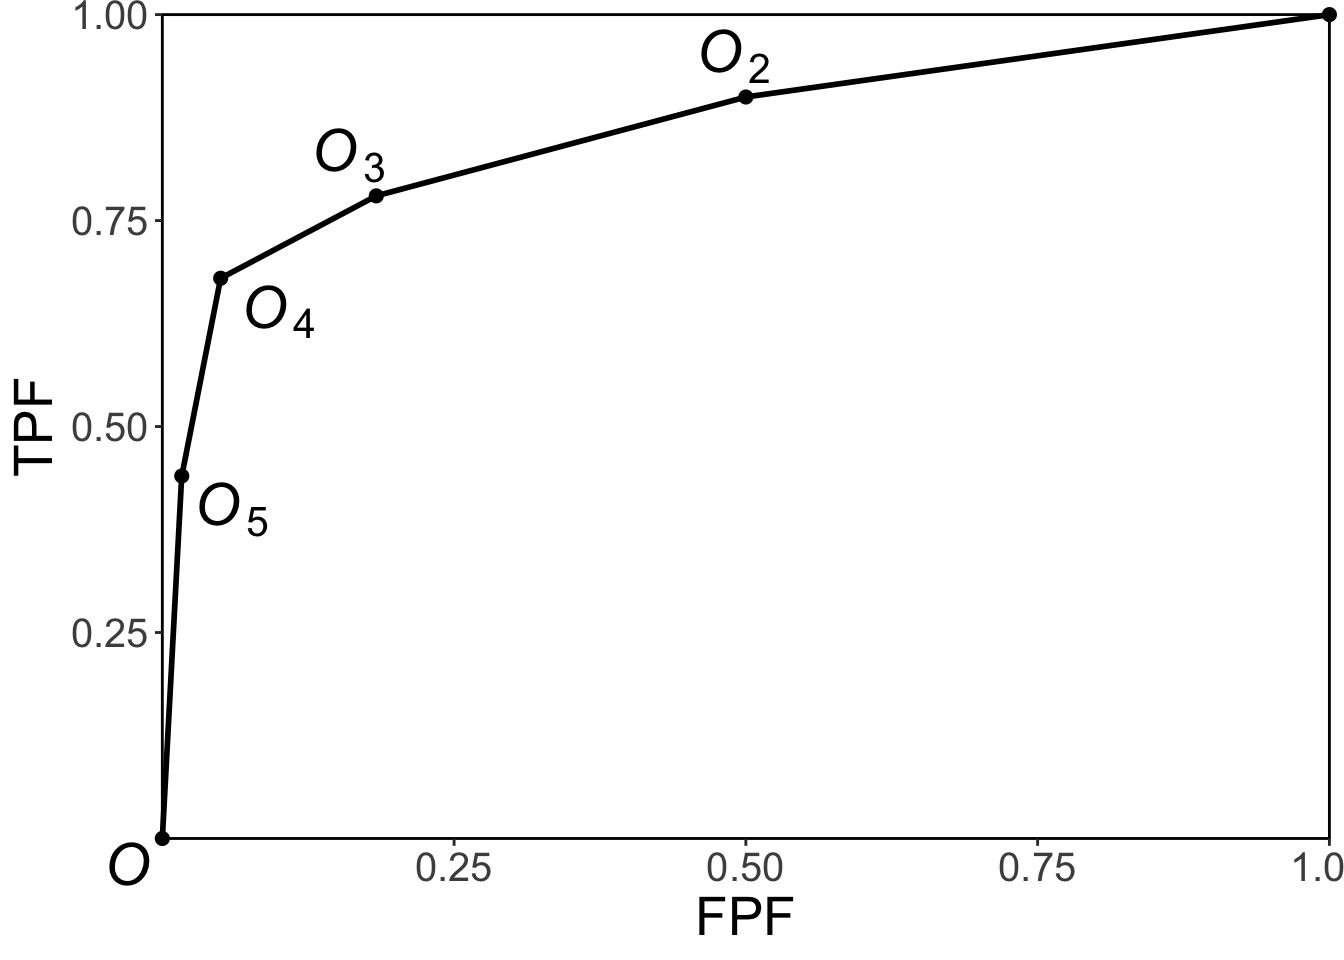
\includegraphics{04-ratings-task_files/figure-latex/ratings-paradigm-labeling-points-figure-1.pdf}
\caption{\label{fig:ratings-paradigm-labeling-points-figure}Operating point labeling convention and the empirical ROC plot.}
\end{figure}

The labeling \(O_n\) of the points follows the following convention, Fig. \ref{fig:ratings-paradigm-labeling-points-figure}: from Eqn. \eqref{eq:ratings-paradigm-FPF-TPF-from-counts} the point \(O_1\) corresponding to \(r=1\) would be the upper right corner (1,1) of the ROC plot, a trivial operating point since it is common to all datasets and is therefore not shown. The labeling starts with the next lower-left point, labeled \(O_2\), which corresponds to \(r=2\); the next lower-left point is labeled \(O_3\), corresponding to \(r=3\), etc., and the point labeled \(O_5\) is the lowest non-trivial operating point corresponding to \(r=5\) and finally \(O_{R+1}\) corresponding to \(r=R+1=6\) is the origin (0,0) of the ROC plot which is also a trivial operating point because it is common to all datasets and is therefore not shown.

\begin{quote}
To summarize, the operating points are labeled starting with the upper right corner, labeled \(O_2\), and working down the curve each time increasing the subscript by one. The maximum number of non-trivial points is \(R-1\).
\end{quote}

\hypertarget{ratings-task-examples}{%
\subsection{Examples}\label{ratings-task-examples}}

In the following examples \(R = 5\) is the number of ROC bins and \(K_{1(R+1)}\) = \(K_{2(R+1)}\) = 0. If \(r = 1\) one gets the uppermost ``trivial'' operating point (1,1):

\begin{equation*} 
FPF_1=\frac {1} {K_1} \sum_{s=1}^{R+1}K_{1s} = \frac{60}{60} = 1\\
TPF_1=\frac {1} {K_2} \sum_{s=1}^{R+1}K_{2s} = \frac{50}{50} = 1
\end{equation*}

The uppermost non-trivial operating point is obtained for \(r = 2\), when:

\begin{equation*} 
FPF_2=\frac {1} {K_1} \sum_{s=2}^{R+1}K_{1s} = \frac{30}{60} = 0.5\\
TPF_2=\frac {1} {K_2} \sum_{s=2}^{R+1}K_{2s} = \frac{45}{50} = 0.9
\end{equation*}

The next lower operating point is obtained for \(r = 3\):

\begin{equation*} 
FPF_3=\frac {1} {K_1} \sum_{s=3}^{R+1}K_{1s} = \frac{11}{60} = 0.183\\
TPF_3=\frac {1} {K_2} \sum_{s=3}^{R+1}K_{2s} = \frac{39}{50} = 0.780
\end{equation*}

The next lower operating point is obtained for \(r = 4\):

\begin{equation*} 
FPF_4=\frac {1} {K_1} \sum_{s=4}^{R+1}K_{1s} = \frac{3}{60} = 0.05\\
TPF_4=\frac {1} {K_2} \sum_{s=4}^{R+1}K_{2s} = \frac{34}{50} = 0.680
\end{equation*}

The lowest non-trivial operating point is obtained for \(r = 5\):

\begin{equation*} 
FPF_5=\frac {1} {K_1} \sum_{s=5}^{R+1}K_{1s} = \frac{1}{60} = 0.017\\
TPF_5=\frac {1} {K_2} \sum_{s=5}^{R+1}K_{2s} = \frac{22}{50} = 0.440
\end{equation*}

The next value \(r = 6\) yields the trivial operating point (0,0):

\begin{equation*} 
FPF_6=\frac {1} {K_1} \sum_{s=6}^{R+1}K_{1s} = \frac{0}{60} = 0\\
TPF_6=\frac {1} {K_2} \sum_{s=6}^{R+1}K_{2s} = \frac{0}{50} = 0
\end{equation*}

This exercise shows explicitly that an R-rating ROC study can yield, at most, \(R + 1\) distinct non-trivial operating points; i.e., those corresponding to \(r=2,3,...,R\).

The modifier ``at most'' is needed, because if both counts (i.e., non-diseased and diseased) for bin \(r'\) are zeroes, then that operating point merges with the one immediately below-left of it:

\begin{equation*} 
FPF_{r'}=\frac {1} {K_1} \sum_{s={r'}}^{R+1}K_{1s} = \frac {1} {K_1} \sum_{s={r'+1}}^{R+1}K_{1s} = FPF_{r'+1}\\
\\
TPF_{r'}=\frac {1} {K_2} \sum_{s={r'}}^{R+1}K_{2s} = \frac {1} {K_2} \sum_{s={r'+1}}^{R+1}K_{2s} = TPF_{r'+1}
\end{equation*}

Since bin \(r'\) is unpopulated, one can re-label the bins to exclude the unpopulated bin, and now the total number of bins is effectively \(R-1\).

Since one is cumulating counts, which cannot be negative, the highest non-trivial operating point resulting from cumulating the 2 through 5 ratings has to be to the upper-right of the next adjacent operating point resulting from cumulating the 3 through 5 ratings. This in turn has to be to the upper-right of the operating point resulting from cumulating the 4 through 5 ratings and finally this has to be to the upper right of the operating point resulting from the 5 ratings. In other words, as one cumulates ratings bins, the operating point must move monotonically up and to the right, or more accurately, the point cannot move down or to the left. If a particular bin has zero counts for non-diseased cases, and non-zero counts for diseased cases, the operating point moves vertically up when this bin is cumulated; if it has zero counts for diseased cases, and non-zero counts for non-diseased cases, the operating point moves horizontally to the right when this bin is cumulated.

\hypertarget{ratings-task-code}{%
\section{Implemention in code}\label{ratings-task-code}}

It is useful to replace the preceding detailed explanation with a simple algorithm, as in the following code (lines 1 - 5):

\begin{Shaded}
\begin{Highlighting}[numbers=left,,]
\FunctionTok{options}\NormalTok{(}\AttributeTok{digits =} \DecValTok{3}\NormalTok{)}
\NormalTok{FPF }\OtherTok{\textless{}{-}}\NormalTok{ OpPts[}\DecValTok{1}\NormalTok{,]}
\NormalTok{TPF }\OtherTok{\textless{}{-}}\NormalTok{ OpPts[}\DecValTok{2}\NormalTok{,]}
\NormalTok{df }\OtherTok{\textless{}{-}} \FunctionTok{data.frame}\NormalTok{(}\AttributeTok{FPF =}\NormalTok{ FPF, }\AttributeTok{TPF =}\NormalTok{ TPF)}
\NormalTok{df }\OtherTok{\textless{}{-}} \FunctionTok{t}\NormalTok{(df)}
\FunctionTok{print}\NormalTok{(df)}
\CommentTok{\#\textgreater{}       [,1] [,2]  [,3] [,4] [,5]}
\CommentTok{\#\textgreater{} FPF 0.0167 0.05 0.183  0.5    1}
\CommentTok{\#\textgreater{} TPF 0.4400 0.68 0.780  0.9    1}
\CommentTok{\# ev = equal variance model}
\NormalTok{mu\_ev }\OtherTok{\textless{}{-}} \FunctionTok{qnorm}\NormalTok{(.}\DecValTok{5}\NormalTok{)}\SpecialCharTok{+}\FunctionTok{qnorm}\NormalTok{(.}\DecValTok{9}\NormalTok{);sigma\_ev }\OtherTok{\textless{}{-}} \DecValTok{1}
\NormalTok{Az\_ev }\OtherTok{\textless{}{-}} \FunctionTok{pnorm}\NormalTok{(mu\_ev}\SpecialCharTok{/}\FunctionTok{sqrt}\NormalTok{(}\DecValTok{2}\NormalTok{))}
\FunctionTok{cat}\NormalTok{(}\StringTok{"uppermost point based estimate of mu\_ev = "}\NormalTok{, mu\_ev, }\StringTok{"}\SpecialCharTok{\textbackslash{}n}\StringTok{"}\NormalTok{)}
\CommentTok{\#\textgreater{} uppermost point based estimate of mu\_ev =  1.28}
\FunctionTok{cat}\NormalTok{(}\StringTok{"corresponding estimate of Az\_ev = "}\NormalTok{, Az\_ev, }\StringTok{"}\SpecialCharTok{\textbackslash{}n}\StringTok{"}\NormalTok{)}
\CommentTok{\#\textgreater{} corresponding estimate of Az\_ev =  0.818}
\end{Highlighting}
\end{Shaded}

Notice that the values of the arrays \texttt{FPF} and \texttt{TPF} are identical to those listed in Table \ref{tab:ratings-paradigm-table-2}. Regarding lines 10 and 11 of code it was shown in Chapter \ref{binary-task} that in the equal variance binormal model the operating point determines the parameters \(\mu_{ev}\) = 1.282, Eqn. \eqref{eq:binary-task-model-solve-mu}, or equivalently \(A_{z;\sigma = 1}\) = 0.818, Eqn. \eqref{eq:binary-task-model-az-var}. These lines illustrate the application of these formulae using the coordinates (0.5, 0.9) of the uppermost non-trivial operating point, i.e., one is fitting the equal variance model to the uppermost operating point.

Shown next is the equal-variance model fit to the uppermost non-trivial operating point, left panel, and for comparison, the right panel is the unequal variance model fit to all operating points (the unequal variance model is described in the next chapter).

\begin{Shaded}
\begin{Highlighting}[]
\CommentTok{\# equal variance fit to uppermost operating point}
\NormalTok{p1 }\OtherTok{\textless{}{-}} \FunctionTok{plotROC}\NormalTok{ (mu\_ev, sigma\_ev, FPF, TPF)}
\CommentTok{\# the following values are from unequal{-}variance model fitting}
\CommentTok{\# to be discussed in the next chapter}
\NormalTok{mu }\OtherTok{\textless{}{-}} \FloatTok{2.17}\NormalTok{;sigma }\OtherTok{\textless{}{-}} \FloatTok{1.65}
\CommentTok{\# following formula is discussed in the next chapter}
\NormalTok{Az }\OtherTok{\textless{}{-}} \FunctionTok{pnorm}\NormalTok{(mu}\SpecialCharTok{/}\FunctionTok{sqrt}\NormalTok{(}\DecValTok{1}\SpecialCharTok{+}\NormalTok{sigma}\SpecialCharTok{\^{}}\DecValTok{2}\NormalTok{))}
\FunctionTok{cat}\NormalTok{(}\StringTok{"binormal unequal variance model estimate of Az = "}\NormalTok{, Az, }\StringTok{"}\SpecialCharTok{\textbackslash{}n}\StringTok{"}\NormalTok{)}
\CommentTok{\#\textgreater{} binormal unequal variance model estimate of Az =  0.87}
\CommentTok{\# unequal variance fit to all operating points}
\NormalTok{p2 }\OtherTok{\textless{}{-}} \FunctionTok{plotROC}\NormalTok{ (mu, sigma, FPF, TPF)}
\end{Highlighting}
\end{Shaded}

\begin{Shaded}
\begin{Highlighting}[]
\FunctionTok{grid.arrange}\NormalTok{(p1,p2,}\AttributeTok{ncol=}\DecValTok{2}\NormalTok{)}
\end{Highlighting}
\end{Shaded}

\begin{figure}
\centering
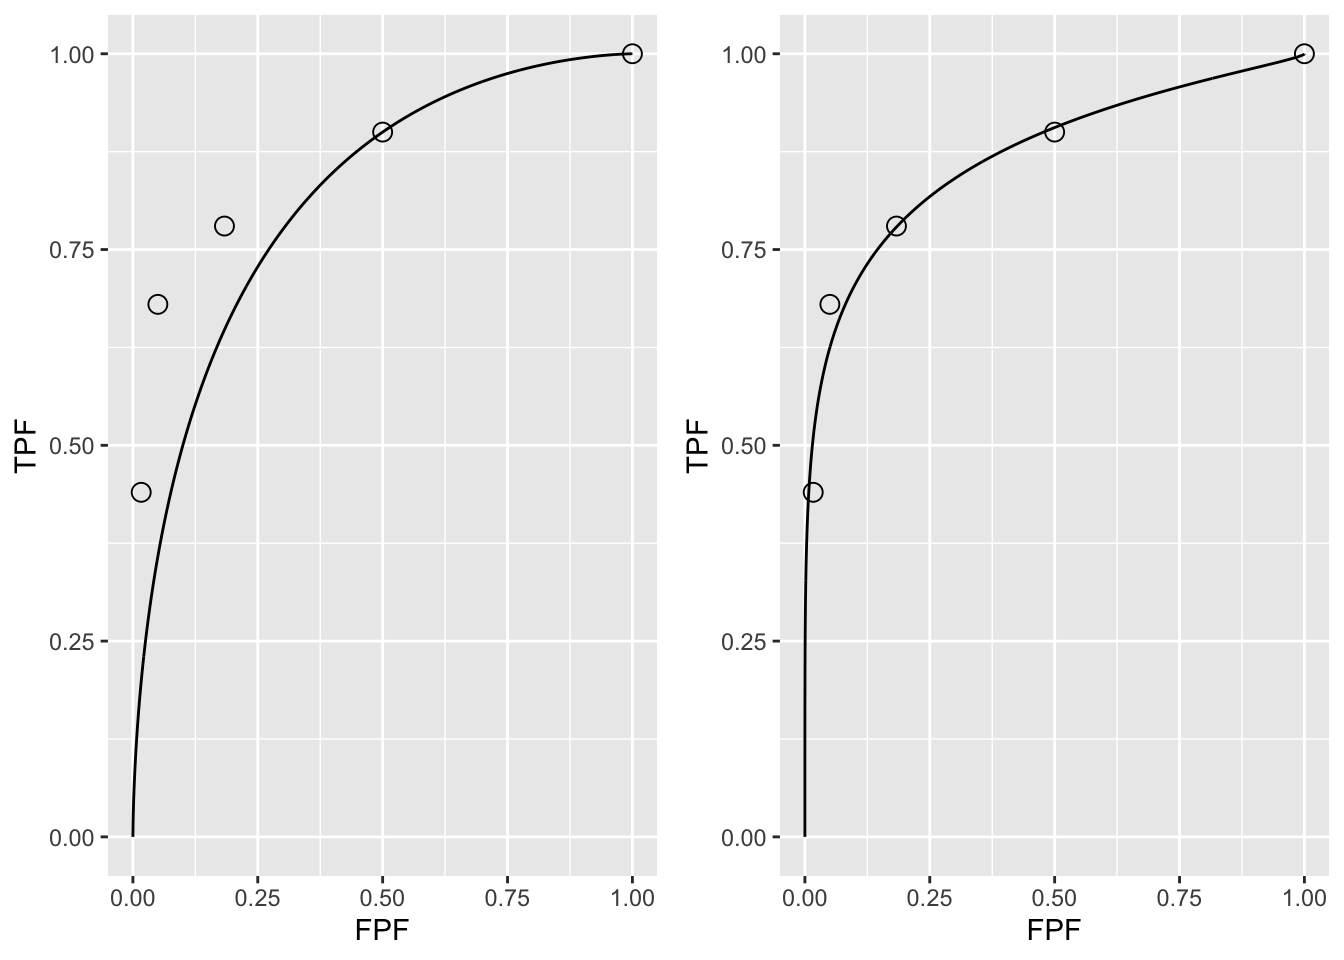
\includegraphics{04-ratings-task_files/figure-latex/ratings-paradigm-eq-var-fit-1.pdf}
\caption{\label{fig:ratings-paradigm-eq-var-fit}A: This panel is the predicted ROC curve for \(\mu=1.28\) superposed on the operating points. B: This panel is the same data fitted with a unequal variance model described in a following chapter.}
\end{figure}

It should come as no surprise that the uppermost operating point in panel A is \emph{exactly} on the predicted curve: after all, this point was used to calculate \(\mu_{ev}\) = 1.282. The corresponding value of \(\zeta\) can be calculated from Eqn. \eqref{eq:binary-task-model-se-sp}, namely:

\begin{equation*} 
\zeta = \Phi^{-1}\left ( Sp \right )
\label{eq:ratings-paradigm-Zeta}
\end{equation*}

\begin{equation*} 
\mu = \zeta + \Phi^{-1}\left ( Se \right )
\label{eq:ratings-paradigm-Mu}
\end{equation*}

These are coded below:

\begin{Shaded}
\begin{Highlighting}[]
\CommentTok{\# Sp = 1 {-} FPF = 1 {-} 0.5}
\CommentTok{\# Se = 0.9}
\FunctionTok{cat}\NormalTok{(}\StringTok{"zeta from Sp = "}\NormalTok{, }\FunctionTok{qnorm}\NormalTok{(}\DecValTok{1}\FloatTok{{-}0.5}\NormalTok{),}\StringTok{"}\SpecialCharTok{\textbackslash{}n}\StringTok{"}\NormalTok{)}
\CommentTok{\#\textgreater{} zeta from Sp =  0}
\FunctionTok{cat}\NormalTok{(}\StringTok{"zeta from Se = "}\NormalTok{, mu\_ev}\SpecialCharTok{{-}}\FunctionTok{qnorm}\NormalTok{(}\FloatTok{0.9}\NormalTok{),}\StringTok{"}\SpecialCharTok{\textbackslash{}n}\StringTok{"}\NormalTok{)}
\CommentTok{\#\textgreater{} zeta from Se =  0}
\end{Highlighting}
\end{Shaded}

Either way, one gets the same result: \(\zeta\) = 0. This should make sense as FPF = 0.5 is consistent with half of the (symmetrical) unit-normal non-diseased distribution being above \(\zeta\) = 0.

Exercise: calculate \(\zeta\) for each of the remaining operating points. Notice that \(\zeta\) increases as one moves down the curve.

\begin{itemize}
\item
  In Fig. \ref{fig:ratings-paradigm-eq-var-fit} panel A show that the ROC curve, as determined by the uppermost operating point, passes exactly through this point but misses the others. If a different operating point were used to estimate \(\mu_{ev}\) and \(A_{z;\sigma = 1}\) the values would have been different and the new curve would pass exactly through the new selected point. No single-point based choice of \(\mu{ev}\) would yield a satisfactory visual fit to all the observed operating points. This is the reason one needs a modified model, namely the unequal variance binormal model, to fit radiologist data.
\item
  Fig. \ref{fig:ratings-paradigm-eq-var-fit} panel B shows the predicted ROC curve by the unequal variance binormal model, to be introduced in a following chapter. The corresponding parameter values are \(\mu\) = 2.17 and \(\sigma\) = 1.65.
\item
  Notice the improved visual quality of the fit, especially if one keeps in mind that each observed point is subject to sampling variability, see Eqn. \eqref{eq:binary-task-model-ci-fpf} and Eqn. \eqref{eq:binary-task-model-ci-tpf}. \footnote{The estimates in the preceding chapter were for a single operating point. Since the multiple operating points discussed here are correlated --- some of the counts used to calculate them are common to two or more operating points --- the method described in the previous chapter overestimates the confidence intervals. A modeling approach accounts for these correlations and yields narrower confidence intervals.}
\end{itemize}

\hypertarget{ratings-task-relation-binary-to-rating}{%
\section{Relation between ratings paradigm and the binary paradigm}\label{ratings-task-relation-binary-to-rating}}

Table \ref{tab:ratings-paradigm-example-table} and Table \ref{tab:ratings-paradigm-table-2} correspond to \(R = 5\). In Chapter \ref{binary-task} it was shown that the binary task requires a single fixed threshold parameter \(\zeta\) and a binning rule Eqn. \eqref{eq:ratings-paradigm-binning-rule}: if \(z > \zeta\) assign a rating of 2 and otherwise assign a rating of 1.

\begin{quote}
The R-rating task can be viewed as \(R-1\) simultaneously conducted binary tasks each with its own fixed threshold \(\zeta_r\), where r = 1, 2, \ldots, R-1. It is efficient compared to \(R-1\) sequentially conducted binary tasks; however, the onus is on the observer to maintain fixed-multiple thresholds through the duration of the study.
\end{quote}

The rating method is a more efficient way of collecting the data compared to running the study repeatedly with appropriate instructions to cause the observer to adopt different fixed thresholds. In the clinical context such repeated studies would be impractical because it would introduce memory effects wherein the diagnosis of a case would depend on how many times the case had been seen in previous sessions.

In order to model the binning, one defines dummy thresholds \(\zeta_0 = - \infty\) and \(\zeta_R = + \infty\), in which case the thresholds satisfy the ordering requirement \(\zeta_{r-1} \le \zeta_r\) , r = 1, 2, \ldots, R. The rating or binning rule is:

\begin{equation}
\left.
\begin{aligned}  
\text{if} \left (\zeta_{r-1} \le z < \zeta_r  \right )&\Rightarrow \text{rating} = r\\
&r = 1, 2, ..., R
\end{aligned}
\right \}
\label{eq:ratings-paradigm-binning-rule}
\end{equation}

For Table \ref{tab:ratings-paradigm-table-2}, the \textbf{empirical} thresholds are as follows:

\begin{equation} 
\left.
\begin{aligned}
\zeta_r &= r + 1 \\
r &= 0, 1, ..., R-1\\
\zeta_0 &= -\infty\\
\zeta_R &= \infty\\
\end{aligned}
\right \}
\label{eq:ratings-paradigm-empirical-zeta}
\end{equation}

The empirical thresholds are integers, not floating point values predicted by Eqn. \eqref{eq:ratings-paradigm-Zeta}. Either way one gets the same operating points. This is a subtle and important distinction explained further in the next section.

In Table \ref{tab:ratings-paradigm-example-table} the number of bins is \(R = 5\). The ``simultaneously conducted binary tasks'' nature of the rating task can be appreciated from the following examples. Suppose one selects the threshold for the first binary task to be \(\zeta_4 = 5\). By definition, \(\zeta_5 = \infty\); therefore a case rated 5 satisfies the binning rule \(\zeta_4 \leq 5 < \zeta_5\), i.e., Eqn. \eqref{eq:ratings-paradigm-binning-rule}. The operating point corresponding to \(\zeta_4 = 5\), obtained by cumulating all cases rated five, yields \((0.017, 0.440)\). In the second binary-task, one selects as threshold \(\zeta_3 = 4\). Therefore, a case rated four satisfies the binning rule \(\zeta_3 \leq 4 < \zeta_4\). The operating point corresponding to \(\zeta_3 = 4\), obtained by cumulating all cases rated four or five, yields \((0.05, 0.680)\). Similarly, for \(\zeta_2 = 3\), \(\zeta_1 = 2\) and \(\zeta_0 = -\infty\), which cumulates counts in bins 3, 2 and 1, respectively. The 1-bin yields a trivial operating point (1,1). The non-trivial operating points are generated by thresholds \(\zeta_r\), where \(r\) = 1, 2, 3 and 4. A five-rating study has four associated thresholds and a corresponding number of equivalent binary studies.

\hypertarget{binary-task-ratings-not-numerical-values}{%
\section{Ratings are not numerical values}\label{binary-task-ratings-not-numerical-values}}

\begin{quote}
The ratings are to be thought of as ordered labels, not as numeric values. Arithmetic operations that are allowed on numeric values, such as averaging, are not allowed on ratings. One could have relabeled the ratings in Table 4.2 as A, B, C, D and E, where A \textless{} B etc. As long as the counts in the body of the table are unaltered, such relabeling would have no effect on the observed operating points and the fitted curve. Of course one cannot average the labels A, B, etc. of different cases. The issue with numeric labels is not fundamentally different. At the root is that the difference in thresholds corresponding to the different operating points are not in relation to the difference between their numeric values. There is a way to estimate the underlying thresholds, if one assumes a specific model, for example the unequal-variance binormal model to be described in Chapter 06. The thresholds so obtained are genuine numeric values and can be averaged. {[}Not to hold the reader in suspense, the four thresholds corresponding to the data in Table 4.1 are 0.007676989, 0.8962713, 1.515645 and 2.396711; see §6.4.1; these values would be unchanged if, for example, the labels were doubled, with allowed values 2, 4, 6, 8 and 10, or any of an infinite number of rearrangements that preserves their ordering.{]}
\end{quote}

The temptation to regard confidence levels / ratings as numeric values can be particularly strong when one uses a large number of bins to collect the data. One could use of quasi-continuous ratings scale, implemented for example, by having a slider-bar user interface for selecting the rating. The slider bar typically extends from 0 to 100, and the rating could be recorded as a floating-point number, e.g., 63.45. Here too one cannot assume that the difference between a zero-rated case and a 10 rated case is a tenth of the difference between a zero-rated case and a 100 rated case. So averaging the ratings is not allowed. Additionally, one cannot assume that different observers use the labels in the same way. One observer's 4-rating is not equivalent to another observers 4-rating.

\begin{quote}
Working directly with the ratings is a very bad idea: valid analytical methods use the rankings of the ratings, not their actual values. The reason for the emphasis is that there are serious misconceptions about ratings. I am aware of a publication stating, to the effect, that a modality resulted in an increased average confidence level for diseased cases. Another publication used a specific numerical value of a rating to calculate the operating point for each observer -- this assumes all observers use the rating scale in the same way, which they do not.
\end{quote}

\hypertarget{binary-task-clinical-operating-point}{%
\section{A single ``clinical'' operating point from ratings data}\label{binary-task-clinical-operating-point}}

The reason for the quotes in the title to this section is that a single operating point on a laboratory ROC plot, no matter how obtained, has little relevance to how radiologists operate in the clinic. However, some consider it useful to quote an operating point from an ROC study. For a 5-rating ROC study, Table \ref{tab:ratings-paradigm-example-table}, it is not possible to unambiguously calculate the operating point of the observer in the binary task of discriminating between non-diseased and diseased cases. One possibility would be to use the ``three and above'' ratings to define the operating point, but one might jus have well have chosen ``two and above''. A second possibility is to instruct the radiologist that a ``four and above'' rating, for example, implies the case would be reported ``clinically'' as diseased. However, the radiologist can only pretend so far that this study, which has no clinical consequences, is somehow a ``clinical'' study.

If a single laboratory study based operating point is desired \citep{RN2660}, the best strategy, in my opinion, is to obtain the rating via two questions. This method is also illustrated in Table 3.1 of a book on detection theory \citep{macmillan2004detection}. The first question is ``is the case diseased?'' The binary (Yes/No) response to this question allows unambiguous calculation of the operating point. The second question is: ``what is your confidence in your previous decision?'' and allow three responses, namely Low, Medium and High. The dual-question approach is equivalent to a 6-point rating scale, Fig. \ref{fig:SixPointScale}. The answer to the first question, is the patient diseased, allows unambiguous construction of a single ``clinical'' operating point for disease presence. The answer to the second question yields multiple operating points.

\begin{figure}

{\centering 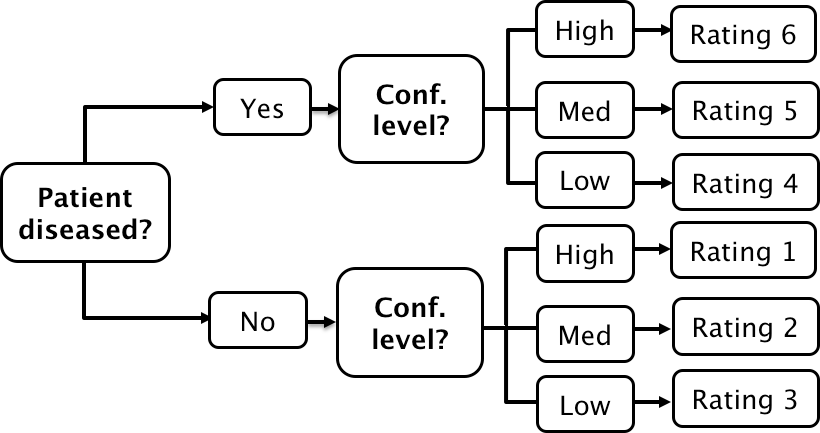
\includegraphics[width=11.39in]{images/AcquiringData6PointScale} 

}

\caption{A method for acquiring ROC data on an effectively 6-point scale that also yields an unambiguous single operating point for declaring patients diseased. Note the reversal of the ordering of the final ratings in the last "column" in the lower half of the figure.}\label{fig:SixPointScale}
\end{figure}

The ordering of the ratings can be understood as follows. The four, five and six ratings are as expected. If the radiologist states the patient is diseased and the confidence level is high that is clearly the highest end of the scale, i.e., six, and the lower confidence levels, five and four, follow, as shown. If, on the other hand, the radiologist states the patient is non-diseased, and the confidence level is high, then that must be the lowest end of the scale, i.e., ``1''. The lower confidence levels in a negative decision must be higher than ``1'', namely ``2'' and ``3'', as shown. As expected, the low confidence ratings, namely ``3'' (non-diseased, low confidence) and ``4'' (diseased, low confidence) are adjacent to each other. With this method of data-collection, there is no confusion as to what rating defines the single desired operating point as this is determined by the binary response to the first question. The 6-point rating scale is also sufficiently fine to not smooth out the ability of the radiologist to maintain distinct different levels. In my experience, using this scale one expects rating noise of about \(\pm\frac{1}{2}\) a rating bin, i.e., the same difficult case, shown on different occasions to the same radiologist (with sufficient time lapse or other intervening cases to minimize memory effects) is expected to elicit a ``3'' or ``4'', with roughly equal probability.

\hypertarget{binary-task-2afc}{%
\section{The forced choice paradigm}\label{binary-task-2afc}}

In each of the four paradigms (ROC, FROC, LROC and ROI) described in Chapter \ref{preliminaries-intro}, patient images are displayed one patient at a time. A fifth paradigm involves presentation of multiple images simultaneously to the observer, where one image is from a diseased patient, and the rest are from non-diseased patients. The observer's task is to pick the image that is most likely to be from the diseased patient. If the observer is correct, the event is scored as a ``one'' and otherwise it is scored as a ``zero''. The process is repeated with other sets of independent patient images, each time satisfying the condition that one patient is diseased and the rest are non-diseased. The sum of the scores divided by the total number of scores is the probability of a correct choice, denoted \(P(C)\). If the total number of cases presented at the same time is denoted \(n\), then the task is termed n-alternative forced choice or nAFC \citep{green1966signal}. If only two cases are presented, one diseased and the other non-diseased, then n = 2 and the task is 2AFC. In Fig. \ref{fig:2AFC}, in the left image a Gaussian nodule is superposed on a square region extracted from a non-diseased mammogram. The right image is a region extracted from a different non-diseased mammogram (one should not use the same background in the two images -- the analysis assumes that different, i.e., independent images, are shown). If the observer clicks on the left image, a correct choice is recorded. {[}In some 2AFC-studies, the backgrounds are simulated non-diseased images. They resemble mammograms; the resemblance depends on the expertise of the observer: expert radiologists can tell that they are not true mammograms. They are actually created by filtering the random white noise with a \(1/f^3\) spatial filter \citep{burgess2011visual}.{]}

The 2AFC paradigm is popular because its analysis is straightforward and there is a theorem \citep{green1966signal} that \(P(C)\), the probability of a correct choice in the 2AFC task equals the area under the true (not fitted, not empirical) ROC curve. Another reason for its popularity is possibly the speed at which data can be collected, sometimes only limited by the speed at which disk stored images can be displayed on the monitor. While useful for studies into human visual perception on relatively simple images, and the model observer community has performed many studies using this paradigm, I cannot recommend it for clinical studies because it does not resemble any clinical task. Additionally, the forced-choice paradigm is wasteful of known-truth images, often a difficult/expensive resource to come by, because narrower confidence intervals are obtained using the ratings ROC method or by utilizing location specific extensions of the ROC paradigm.

\begin{figure}

{\centering 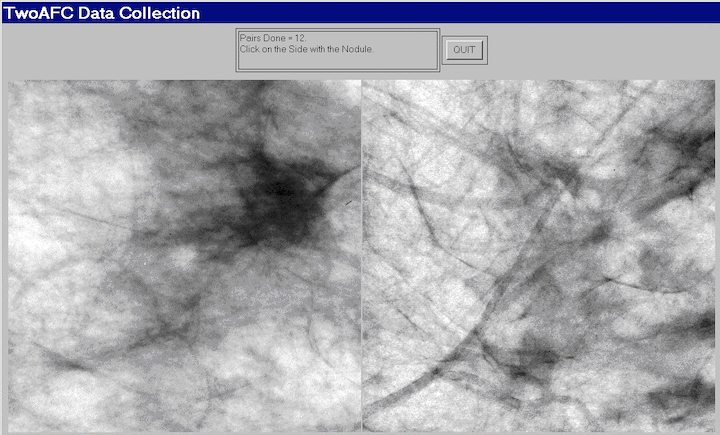
\includegraphics[width=10in]{images/2AFC} 

}

\caption{Example of image presentation in a 2AFC study.}\label{fig:2AFC}
\end{figure}

Fig. \ref{fig:2AFC}: Example of image presentation in a 2AFC study. The left image contains, at its center, a positive contrast Gaussian shape disk superposed on a non-diseased mammogram. The right image does not contain a lesion at its center and the background is from a different non-diseased patient. If the observer clicks on the left image it is recorded as a correct choice, otherwise it is recorded as an incorrect choice. The number of correct choices divided by the number of paired presentations is an estimate of the probability of a correct choice, which can be shown to be identical to the true area under the ROC curve.

\hypertarget{binary-task-observer-studies-as-simulations}{%
\section{Observer performance studies as laboratory simulations of clinical tasks}\label{binary-task-observer-studies-as-simulations}}

\begin{itemize}
\item
  Observer performance paradigms (ROC, FROC, LROC and ROI) should be regarded as experiments conducted in a laboratory (i.e., controlled) setting that are intended to be representative of the actual clinical task. They should not to be confused with performance in a real ``live'' clinical setting: there is a known ``laboratory effect'' \citep{RN2026}. For example, in the just cited study radiologists performed better during live clinical interpretations than they did later, on the same cases, in a laboratory ROC study. This is to be expected because there is more at stake during live interpretations: e.g., the patient's health and the radiologist's reputation, than during laboratory ROC studies.
\item
  Real clinical interpretations happen every day in radiology departments all over the world. On the other hand, in the laboratory, the radiologist is asked to interpret the images ``as if in a clinical setting'' and render a ``diagnosis''. The laboratory decisions have no clinical consequences. Usually laboratory ROC studies are conducted on retrospectively acquired images. Patients, whose images are used in an ROC study, have already been imaged in the clinic and decisions have already been made on how to manage them.
\item
  There is no guarantee that results of the laboratory study are directly applicable to clinical practice. Indeed there is an assumption that the laboratory study correlates with clinical performance. The correlation is taken to be an axiomatic truth by researchers when, in fact, it is an assumption.
\item
  This section should not be interpreted as expressing my lack of trust in laboratory studies. Simulations are widely used in ``hard'' sciences, e.g., they are used in astrophysics to determine conditions dating to \(10^{-31}\) seconds after the big bang. Conducting clinical studies is very difficult as there are many factors not under the researcher's control. Observer performance studies of the type described in this book are the closest that one can come to the ``real thing'' as they include key elements of the actual clinical task: the entire imaging system, radiologists (assuming the radiologists' brings their full expertise to bear on each image interpretation) and real clinical images.
\end{itemize}

\hypertarget{binary-task-discrete-vs-continuous-ratings}{%
\section{Discrete vs.~continuous ratings: the Miller study}\label{binary-task-discrete-vs-continuous-ratings}}

\begin{itemize}
\item
  There is controversy about the merits of discrete vs.~continuous ratings \citep{rockette1992use, wagner2001continuous}. The late Prof.~Charles E. Metz and the late Dr.~Robert F. Wagner have both backed the latter (i.e., continuous or quasi-continuous ratings) and new ROC study designs sometimes tend to follow their advice. I recommend a 6-point rating scale as outlined in Fig. \ref{fig:SixPointScale}. This section provides the background for the recommendation.
\item
  A widely cited (39,704 citations at the time of writing, ca. March 2023) paper by Miller \citep{miller1956magical} titled ``The Magical Number Seven, Plus or Minus Two: Some Limits on Our Capacity for Processing Information'' is relevant. It is a readable paper, freely downloadable in several languages (www.musanim.com/miller1956/). In my judgment, this paper has not received the attention it should have in the ROC community, and for this reason portions from it are reproduced below. {[}George Armitage Miller, February 3, 1920 -- July 22, 2012, was one of the founders of the field of cognitive psychology.{]}
\item
  Miller's first objective was to comment on absolute judgments of unidimensional stimuli. Since all (univariate, i.e., single decision per case) ROC models assume a unidimensional decision variable, Miller's work is highly relevant. He comments on two papers by Pollack \citep{pollack1952information, pollack1953information}. Pollack asked listeners to identify tones by assigning numerals to them, analogous to a rating task described above. The tones differed in frequency, covering the range 100 to 8000 Hz in equal logarithmic steps. A tone was sounded and the listener responded by giving a numeral (i.e., a rating, with higher values corresponding to higher frequencies). After the listener had made his response, he was told the correct identification of the tone. When only two or three tones were used, the listeners never confused them. With four different tones, confusions were quite rare, but with five or more tones, confusions were frequent. With fourteen different tones, the listeners made many mistakes. Since it is so succinct, the entire content of the first (1952) paper by Pollack is reproduced below:
\end{itemize}

\begin{quote}
``In contrast to the extremely acute sensitivity of a human listener to discriminate small differences in the frequency or intensity between two sounds is his relative inability to identify (and name) sounds presented individually. When the frequency of a single tone is varied in equal‐logarithmic steps in the range between 100 cps and 8000 cps (and when the level of the tone is randomly adjusted to reduce loudness cues), the amount of information transferred is about 2.3 bits per stimulus presentation. This is equivalent to perfect identification among only 5 tones. The information transferred, under the conditions of measurement employed, is reasonably invariant under wide variations in stimulus conditions.''
\end{quote}

\begin{itemize}
\item
  By ``information'' is meant the number of levels, measured in bits (binary digits), thereby making it independent of the unit of measurement: 1 bit corresponds to a binary rating scale, 2 bits to a four-point rating scale and 2.3 bits to \(2^{2.3}\) = 4.9, i.e., about 5 ratings bins. Based on Pollack's' original unpublished data, Miller put an upper limit of 2.5 bits (corresponding to about 6 ratings bins) on the amount of information that is transmitted by listeners who make absolute judgments of auditory pitch. The second paper \citep[@][]{pollack1953information} by Pollack was related to: (1) the frequency range of tones; (2) the utilization of objective reference tones presented with the unknown tone; and (3) the ``dimensionality''---the number of independently varying stimulus aspects. Little additional gain in information transmission was associated with the first factor; a moderate gain was associated with the second; and a relatively substantial gain was associated with the third (we return to the dimensionality issue below).
\item
  As an interesting side-note, Miller states:
\end{itemize}

\begin{quote}
``Most people are surprised that the number is as small as six. Of course, there is evidence that a musically sophisticated person with absolute pitch can identify accurately any one of 50 or 60 different pitches. Fortunately, I do not have time to discuss these remarkable exceptions. I say it is fortunate because I do not know how to explain their superior performance. So I shall stick to the more pedestrian fact that most of us can identify about one out of only five or six pitches before we begin to get confused.''
\end{quote}

\begin{quote}
``It is interesting to consider that psychologists have been using seven-point rating scales for a long time on the intuitive basis that trying to rate into finer categories does not really add much to the usefulness of the ratings. Pollack's results indicate that, at least for pitches, this intuition is fairly sound.''
\end{quote}

\begin{quote}
``Next you can ask how reproducible this result is. Does it depend on the spacing of the tones or the various conditions of judgment? Pollack varied these conditions in a number of ways. The range of frequencies can be changed by a factor of about 20 without changing the amount of information transmitted more than a small percentage. Different groupings of the pitches decreased the transmission, but the loss was small. For example, if you can discriminate five high-pitched tones in one series and five low-pitched tones in another series, it is reasonable to expect that you could combine all ten into a single series and still tell them all apart without error. When you try it, however, it does not work. The channel capacity for pitch seems to be about six and that is the best you can do.''
\end{quote}

\begin{itemize}
\item
  DPC comment: I was unable to find a single study in the medical imaging field of the number of discrete rating levels that an observer can support.
\item
  There is no question that for multidimensional data, as observed in the second study by Pollack \citep{pollack1953information}, the observer can support more than 7 ratings bins. To quote Miller:
\end{itemize}

\begin{quote}
``You may have noticed that I have been careful to say that this magical number seven applies to one-dimensional judgments. Everyday experience teaches us that we can identify accurately any one of several hundred faces, any one of several thousand words, any one of several thousand objects, etc. The story certainly would not be complete if we stopped at this point. We must have some understanding of why the one-dimensional variables we judge in the laboratory give results so far out of line with what we do constantly in our behavior outside the laboratory. A possible explanation lies in the number of independently variable attributes of the stimuli that are being judged. Objects, faces, words, and the like differ from one another in many ways, whereas the simple stimuli we have considered thus far differ from one another in only one respect.''
\end{quote}

\begin{itemize}
\item
  DPC comment: In the medical imaging context, a trivial way to increase the number of ratings would be to color-code the images: e.g., red, green and blue; now one can assign a red image rated 3, a green image rated 2, etc., which would be meaningless unless the colors encode relevant diagnostic information. Another ability, quoted in the publication \citep{wagner2001continuous} advocating continuous ratings is the ability to recognize faces, again a multidimensional categorization task, addressed by Miller (see above). Also quoted as an argument for continuous ratings is the ability of computer aided detection schemes that calculate many features for each perceived lesion and combine them into a single probability of malignancy, which is on a highly precise floating point 0 to 1 scale. Radiologists are not computers. Other arguments for greater number of bins: it cannot hurt and one should acquire the rating data at greater precision than the noise, especially if the radiologist is able to maintain the finer distinctions. I worry that radiologists who are willing to go along with greater precision are over-anxious to co-operate with the study designer. Expert radiologists will not modify their reading style and one should be suspicious when they do accede to an investigators request to interpret images in a style that does not resemble the clinic. Radiologists, especially experts, do not like more than about four ratings. I once worked closely with a famous chest radiologist (the late Dr.~Robert Fraser) who refused to use more than four ratings. \footnote{Dr.~Fraser famously termed -- off the record -- our statistical analysis in \citep{Chakraborty1986DigitalVsConv} ``gobbledygook''.}
\item
  Another reason given for using continuous ratings is it reduces instances of data degeneracy. Data is sometimes said to be degenerate if the curve-fitting algorithm cannot fit it (in simple terms, the program ``crashes'' or reports unphysical parameter values). This occurs if there are no interior points on the ROC plot. Modifying radiologist behavior to accommodate the limitations of analytical methods seems to be inherently dubious. One could simply randomly add or subtract half an integer from the observed ratings thereby making the rating scale more granular and thus reduce instances of degeneracy (this is actually done in some ROC software to overcome this problem). Another possibility is to use the empirical (trapezoidal) area under the ROC curve, which can always be calculated. Actually, fitting methods now exist that are robust to data degeneracy, such as discussed in Chapter \texttt{TempComment\ \textbackslash{}@ref(proper-roc-models)} and in the RSM fitting chapter in TBA \texttt{RJafrocFrocBook}, so this reason for acquiring continuous data is no longer valid.
\item
  The rating task involves a unidimensional scale and I see no way of getting around the basic channel-limitation noted by Miller and for this reason I recommend a 6 point scale, as in Fig. \ref{fig:SixPointScale}.
\item
  On the other side of the controversy \citep{berbaum2002empirical}, a position that I agree with, it has been argued that given a large number of allowed ratings levels the cooperating observer essentially bins the data into a much smaller number of bins (e.g., 0, 20, 40, 60, 80, 100) and then adds a zero-mean noise term to appear to be ``spreading out the ratings''. This ensures that the binormal model does not ``crash''. However, if the intent is to get the observer to spread the ratings, so that the binormal model does not ``crash'', a better approach is to use alternate models that do not ``crash'' and are, in fact, very robust with respect to degeneracy of the data.
\end{itemize}

\hypertarget{binary-task-birads-rating-scale}{%
\section{The BI-RADS ratings scale and ROC studies}\label{binary-task-birads-rating-scale}}

It is desirable that the rating scale be relevant to the radiologists' daily practice. This assures greater consistency -- the fitting algorithms assume that the thresholds are held constant for the duration of the ROC study. Depending on the clinical task, a natural rating scale may already exist. For example, the American College of Radiology has developed the Breast Imaging Reporting and Data System (BI-RADS) to standardize mammography reporting \citep{liberman2002breast}. There are six assessment categories: category 0 indicates need for additional imaging; category 1 is a negative (clearly non-diseased); category 2 is a benign finding; category 3 is probably benign, with short-interval follow-up suggested; category 4 is a suspicious abnormality for which biopsy should be considered; category 5 is highly suggestive of malignancy and appropriate action should be taken. The 4th edition of the BI-RADS manual divides category 4 into three subcategories 4A, 4B and 4C and adds category 6 for a proven malignancy. The 3-category may be further subdivided into ``probably benign with a recommendation for normal or short-term follow-up'' and a 3+ category, ``probably benign with a recommendation for immediate follow-up''. Apart from categories 0 and 2, the categories form an ordered set with higher categories representing greater confidence in presence of cancer. How to handle the 0s and the 2s is the subject of some controversy, described next.

\hypertarget{binary-task-birads-rating-scale-controversy}{%
\subsection{The controversy}\label{binary-task-birads-rating-scale-controversy}}

Two large clinical studies have been reported in which BI-RADS category data were acquired for \textgreater{} 400,00 screening mammograms interpreted by many (124 in the 1st study) radiologists \citep{barlow2004accuracy, fenton2007influence}. The purpose of the first study was to relate radiologist characteristics to actual performance (e.g., does performance depend on reading volume -- the number of cases interpreted per year), so it could be regarded as a more elaborate version of \citep{beam1996variability}, described in Chapter \ref{binary-task}. The purpose of the second study was to determine the effectiveness of computer-aided detection (CAD) in screening mammography.

The reported ROC analyses used the BIRADS assessments labels ordered as follows: \(1 < 2 < 3 < 3+ < 0 < 4 < 5\). The last column of Table \ref{tab:BIRADS-study} shows that with this ordering the numbers of cancer per 1000 patients increases monotonically. The CAD study is discussed later, for now the focus is on the adopted BIRADS scale ordering that is common to both studies and which has raised controversy.

\begin{table}

\caption{\label{tab:BIRADS-study}The Barlow et al study: the ordering of the BI-RADS ratings in the first column correlates with cancer-rate in the last column.}
\centering
\resizebox{\linewidth}{!}{
\begin{tabular}[t]{>{\raggedright\arraybackslash}p{11em}|>{\raggedright\arraybackslash}p{8em}|>{\raggedright\arraybackslash}p{8em}|>{\raggedright\arraybackslash}p{8em}|>{\raggedright\arraybackslash}p{8em}}
\hline
  & Total number 
of mammograms & Mammograms without 
breast cancer (percent) & Mammograms with 
breast cancer  (percent) & Cancers per 1000 
screening mammograms\\
\hline
1: Normal & 356,030 & 355,734 (76.2) & 296 (12.3) & 0.83\\
\hline
2: Benign finding & 56,614 & 56,533 (12.1) & 81 (3.4) & 1.43\\
\hline
3: Probably benign, 
recommend normal or short term follow up & 8,692 & 8,627 (1.8) & 65 (2.7) & 7.48\\
\hline
3+: Probably benign, 
recommend immediate follow up & 3,094 & 3,049 (0.7) & 45 (1.9) & 14.54\\
\hline
0: Need additional 
imaging evaluation & 42,823 & 41,442 (8.9) & 1,381 (57.5) & 32.25\\
\hline
4: Suspicious finding, 
biopsy should be considered & 2,022 & 1,687 (0.4) & 335 (13.9) & 165.68\\
\hline
5: Highly suggestive 
of malignancy & 237 & 38 (0.0) & 199 (8.3) & 839.66\\
\hline
\end{tabular}}
\end{table}

The use of the BI-RADS ratings shown in Table \ref{tab:BIRADS-study} has been criticized \citep{RN2166} in an editorial titled:

\begin{quote}
BI-RADS Data Should Not Be Used to Estimate ROC Curves
\end{quote}

Since BI-RADS is a clinical rating scheme widely used in mammography, the editorial, if correct, implies that ROC analysis of clinical mammography data is not possible. Since the BI-RADS scale was arrived at after considerable deliberation, the inability to perform ROC analysis with it would strike at the root of clinical utility of the ROC method. The purpose of this section is to express the reasons why I have a different take on this controversy.

It is claimed in the editorial that the Barlow et al.~study confuses cancer yield with confidence level and that BI-RADS categories 1 and 2 should not be separate entries of the confidence scale, because both indicate no suspicion for cancer.

I agree with the Barlow et al.~suggested ordering of the ``2s'' as more likely to have cancer than the ``1s''. A category-2 means the radiologist found something to report, and the location of the finding is part of the clinical report. Even if the radiologist believes the finding is definitely benign, there is a non-zero probability that a category-2 finding is cancer, as evident in the last column of Table \ref{tab:BIRADS-study} (\(1.43 > 0.83\)). In contrast, there are no findings associated with a category-1 report. A paper \citep{hartmann2005benign} titled:

\begin{quote}
Benign breast disease and the risk of breast cancer
\end{quote}

should convince any doubters that benign lesions do have a finite chance of cancer.

The problem with ``where to put the 0s'' arises only when one tries to analyze clinical BI-RADS data. In a laboratory study the radiologist would not be given the category-0 option. In analyzing a clinical study it is incumbent on the study designer to justify the choice of the rating scale adopted. Showing that the proposed ordering agrees with the probability of cancer is justification -- and in my opinion, given the very large sample size this was accomplished convincingly in the Barlow et al.~study.

\begin{quote}
Moreover, the last column of Table \ref{tab:BIRADS-study} suggests that any other ordering would violate an important principle, namely, optimal ordering is achieved when each case is rated according to it's likelihood ratio (defined as the probability of the case being diseased divided by the probability of the case being non-diseased). The likelihood ratio is the ``betting odds'' of the case being diseased, which is expected to be monotonic with the empirical probability of the case being diseased, i.e., the last column of Table \ref{tab:BIRADS-study}. Therefore, the ordering adopted in Table \ref{tab:BIRADS-study} is equivalent to adopting a likelihood ratio scale and any other ordering would not be monotonic with likelihood ratio.
\end{quote}

The likelihood ratio is described in more detail in Chapter \texttt{TempComment\ \textbackslash{}@ref(proper-roc-models)}, which describes ROC fitting methods that yield ``proper'' ROC curves, i.e., ones that have monotonically decreasing slope as the operating point moves up the curve from (0,0) to (1,1) and therefore do not inappropriately cross the chance diagonal. Key to these fitting methods is adoption of a likelihood ratio scale to rank-order cases. The fitting algorithm implemented in PROPROC software \textbf{reorders} confidence levels assumed by the binormal model, Chapter \texttt{TempComment\ \textbackslash{}@ref(proper-roc-models)}, paragraph following TBA Fig. 20.4. This is analogous to the reordering of the clinical ratings based on cancer rates assumed in Table \ref{tab:BIRADS-study}. It is illogical to allow reordering of ratings in software but question the same when done in a principled way by a researcher. As expected, the modeled ROC curves in the Barlow publication, their Fig. 4, show no evidence of improper behavior. This is in contrast to a clinical study (about fifty thousands patients spread over 33 hospitals with each mammogram interpreted by two radiologists) using a non-BIRADS 7-point rating scale which yielded markedly improper ROC curves \citep{pisano2005diagnostic} for the film modality when using ROC ratings (not BIRADS). This suggests that use of a non-clinical ratings scale for clinical studies, without independent confirmation of the ordering implied by the scale, is problematical.

The reader might be interested as to reason for the 0-ratings being more predictive of cancer than a 3+ rating, Table \ref{tab:BIRADS-study}. In the clinic the zero rating implies, in effect, ``defer decision, incomplete information, additional imaging necessary''. A zero rating could be due to technical problems with the images: e.g., improper positioning (e.g., missing breast tissue close to the chest wall) or incorrect imaging technique (improper selection of kilovoltage and/or tube charge) making it impossible to properly interpret the images. Since the images are part of the permanent patient record, there are both healthcare and legal reasons why the images need to be optimal. Incorrect technical factors are expected to occur randomly and therefore not predictive of cancer. However, if there is a suspicious finding and the image quality is sub-optimal, the radiologist may be unable to commit to a decision, they may seek additional imaging, perhaps better compression or a slightly different view angle to resolve the ambiguity. Such zero ratings are expected with suspicious findings and are expected to be predictive of cancer.

\hypertarget{ratings-paradigm-discussion}{%
\section{Discussion}\label{ratings-paradigm-discussion}}

In this chapter the widely used ratings paradigm was described and illustrated with a sample dataset. The calculation of ROC operating points from this table was explained. A formal notation was introduced to describe the counts in this table and the construction of operating points and an \texttt{R} example was given. I do not wish to leave the impression that the ratings paradigm is used only in medical imaging. In fact the historical reference \citep{macmillan2004detection} to the two-question six-point scale in Fig. \ref{fig:SixPointScale} was for a rating study on performance in recognizing odors.

While it is possible to use the equal variance binormal model to obtain a measure of performance, the results depend upon the choice of operating point, and evidence was presented for the generally observed fact that most ROC ratings datasets are inconsistent with the equal variance binormal model. This indicates the need for an extended model, to be discussed in Chapter \ref{binormal-model}.

The rating paradigm is a more efficient way of collecting the data compared to repeating the binary paradigm with instructions to cause the observer to adopt different fixed thresholds specific to each repetition. The rating paradigm is also more efficient than the 2AFC paradigm -- and the rating paradigm is more clinically realistic.

Two controversial but important issues were addressed: the reason for my recommendation for adopting a discrete 6-point rating scale and correct usage of clinical BIRADS ratings in ROC studies. When a clinical scale exists, the empirical disease occurrence rate associated with each rating should be used to order the ratings.

The next step is to describe a model for ratings data. Before doing that, it is necessary to introduce an empirical performance measure, namely the area under the empirical or trapezoidal ROC, which does not require any modeling.

\hypertarget{ratings-paradigm-references}{%
\section{Chapter References}\label{ratings-paradigm-references}}

\hypertarget{empirical-auc}{%
\chapter{Empirical AUC}\label{empirical-auc}}

\hypertarget{empirical-auc-how-much-finished}\label{empirical-auc-how-much-finished}}

\hypertarget{empirical-auc-introduction}{%
\section{Introduction}\label{empirical-auc-introduction}}

The ROC plot is defined as the plot of sensitivity (y-axis) vs.~1-specificity (x-axis). Equivalently, it is the plot of \(\text{TPF}\) vs.~\(\text{FPF}\). An equal variance binormal model was introduced in an earlier chapter which allows an ROC plot to be fitted to a single observed operating point. The more commonly used ratings paradigm was introduced in the previous chapter.

It was shown, Fig. \ref{fig:ratings-paradigm-eq-var-fit}, that the equal variance binormal model did not fit a clinical dataset and that an unequal variance binormal model yielded a better visual fit. This turns out to be a general finding. Before getting into the complexity of the unequal variance binormal model curve fitting, see next chapter, it is appropriate to introduce a simpler \textbf{empirical} approach which is very popular with some researchers.

The New Oxford American Dictionary definition of ``empirical'' is:

\begin{quote}
``based on, concerned with, or verifiable by observation or experience rather than theory or pure logic''.
\end{quote}

The empirical method is also termed ``non-parametric'' as it does not involve parametric assumptions (specifically normality assumptions are not needed). Notation is introduced for labeling individual cases. The empirical area under the ROC (AUC) under the empirical plot is defined. An important theorem relating AUC to the Wilcoxon statistic is stated.

\hypertarget{empirical-roc-plot}{%
\section{The empirical ROC plot}\label{empirical-roc-plot}}

\begin{quote}
The empirical ROC plot is constructed by connecting adjacent observed operating points, including the trivial ones at (0,0) and (1,1), with straight lines. The trapezoidal area under this plot is a non-parametric figure of merit that is threshold independent. Since no parametric assumptions are involved some prefer it to parametric methods such as the one to be described in the next chapter.\^{} {[}In the context of AUC, the terms empirical, trapezoidal, or non-parametric all mean the same thing.{]}
\end{quote}

\hypertarget{notation-for-cases}{%
\subsection{Notation for cases}\label{notation-for-cases}}

Cases are indexed by \(k_tt\) where \(t\) indicates the truth-status at the case (i.e., patient) level, with \(t=1\) for non diseased cases and \(t=2\) for diseased cases. Index \(k_1\) ranges from one to \(K_1\) for non-diseased cases and \(k_2\) ranges from one to \(K_2\) for diseased cases where \(K_1\) and \(K_2\) are the total number of non-diseased and diseased cases respectively. In Table \ref{tab:empirical-ROC-2index-notation} each case is represented as a shaded box using lighter shading for non-diseased cases and darker shading for diseased cases. There are 11 non-diseased cases, labeled N1 -- N11, in the upper row of boxes and there are seven diseased cases, labeled D1 -- D7, in the lower row.

\begin{table}

\caption{\label{tab:empirical-ROC-2index-notation}On the need for two indices to label cases in an ROC study.}
\centering
\begin{tabular}[t]{l|l|l|l|l|l|l|l|l|l|l}
\hline
 &  &  &  &  &  &  &  &  &  & \\
\hline
N1 & N2 & N3 & N4 & N5 & N6 & N7 & N8 & N9 & N10 & N11\\
\hline
D1 & D2 & D3 & D4 & D5 & D6 & D7 &  &  &  & \\
\hline
\end{tabular}
\end{table}

To address any cell (i.e., case) in Table \ref{tab:empirical-ROC-2index-notation} one needs two indices: the row number \(t\) and the column number \(k_tt\). Since the column number depends on the value of \(t\) one needs two indices to specify it: specifically, \(k_tt\) denotes the column number \(k_t\) of a case with truth index \(t\). My notation may appear to be unnecessarily liberal in its usage of the \(t\) subscript. Alternative notation commonly uses a single index \(k\) to label the cases. It reserves the first \(K_1\) positions for non-diseased cases and the rest for diseased cases: e.g., \(k = 3\) corresponds to the third non-diseased case, \(k = K_1+5\) corresponds to the fifth diseased case, etc. Because it extends easily to more complex data structures, e.g., FROC, I prefer the two-index notation.

\hypertarget{an-empirical-operating-point}{%
\subsection{An empirical operating point}\label{an-empirical-operating-point}}

Let \(z_{k_tt}\) represent the z-sample of case \(k_tt\). For a given reporting threshold \(\zeta\), and assuming a positive-directed rating scale (i.e., higher values correspond to greater confidence in presence of disease), empirical false positive fraction \(\text{FPF}(\zeta)\) and empirical true positive fraction \(\text{TPF}(\zeta)\) are defined by:

\begin{equation}
\left.
\begin{aligned}
\text{FPF}\left ( \zeta \right ) &= \frac{1}{K_1}\sum_{k_1=1}^{K_1}I\left ( z_{k_11} \geq \zeta \right ) \\
\text{TPF}\left ( \zeta \right ) &= \frac{1}{K_2}\sum_{k_2=1}^{K_2}I\left ( z_{k_22} \geq \zeta \right )
\end{aligned}
\right \}
\label{eq:empirical-auc-op-pt}
\end{equation}

Here \(I(x)\) is the indicator function which equals one if \(x\) is true and is zero otherwise.

In Eqn. \eqref{eq:empirical-auc-op-pt} the indicator functions act as counters effectively counting instances where the z-sample of a case equals or exceeds \(\zeta\), and division by the appropriate denominator yields the desired left hand sides of these equations. The operating point \(O(\zeta)\) corresponding to threshold \(\zeta\) is defined by:

\begin{equation}
O\left ( \zeta \right ) = \left ( \text{FPF}\left ( \zeta \right ), TPF\left ( \zeta \right ) \right )
\label{eq:empirical-operating-point}
\end{equation}

The difference between Eqn. \eqref{eq:empirical-auc-op-pt} and Eqn. \eqref{eq:binary-task-model-fpf-tpf} is that the former is non-parametric while the latter is parametric.

\hypertarget{empirical-auc-operating-points}{%
\section{Empirical operating points from ratings data}\label{empirical-auc-operating-points}}

Consider a ratings ROC study with \(R\) bins. Describing an R-rating empirical ROC plot requires \(R-1\) ordered empirical thresholds, see Eqn. \eqref{eq:ratings-paradigm-empirical-zeta}.

The operating point \(O(\zeta_r)\) is given by:

\begin{equation}
O\left ( \zeta_r \right ) = \left ( \text{FPF}\left ( \zeta_r \right ), TPF\left ( \zeta_r \right ) \right )
\label{eq:empirical-operating-point-zeta-r}
\end{equation}

Its coordinates are defined by:

\begin{equation} 
\left.
\begin{aligned}
\text{FPF}_r \equiv \text{FPF}\left ( \zeta_r \right )=&\frac {1} {K_1} \sum_{k_1=1}^{K_1}I \left ( z_{k_11} \geq  \zeta_r\right ) \\
\text{TPF}_r \equiv \text{TPF}\left ( \zeta_r \right )=&\frac {1} {K_2} \sum_{k_2=1}^{K_2} I\left ( z_{k_22} \geq  \zeta_r\right )
\end{aligned}
\right \}
\label{eq:empirical-operating-point-fpf-tpf}
\end{equation}

For example,

\begin{equation} 
\left.
\begin{aligned}
\text{FPF}_4 \equiv \text{FPF}\left ( \zeta_4 \right )=&\frac {1} {K_1} \sum_{k_1=1}^{K_1}I \left ( z_{k_11} \geq  \zeta_4\right ) \\
\text{TPF}_4 \equiv \text{TPF}\left ( \zeta_4 \right )=&\frac {1} {K_2} \sum_{k_2=1}^{K_2} I\left ( z_{k_22} \geq  \zeta_4\right ) \\
O_4 \equiv \left ( \text{FPF}_4, \text{TPF}_4 \right ) =& \left ( 0.017, 0.44 \right )\\
\end{aligned}
\right \}
\label{eq:empirical-operating-point-fpf-tpf-4}
\end{equation}

Fig. \ref{fig:ratings-paradigm-labeling-points-figure} is the empirical ROC plot. It illustrates the convention used to label the operating points introduced earlier is, i.e., \(O_2\) is the uppermost non-trivial point, and the subscripts increment by unity as one moves down the plot. By convention, not shown are the trivial operating points \(O_0 \equiv (\text{FPF}_0, \text{TPF}_0) = (1,1)\) and \(O_R \equiv (\text{FPF}_R, \text{TPF}_R) = (0,0)\), where \(R = 5\).

\hypertarget{empirical-auc-area-under}{%
\section{AUC under the empirical ROC plot}\label{empirical-auc-area-under}}

Fig. \ref{fig:empirical-auc-empirical-auc} shows the empirical plot for the data in Table 4.1. The area under the curve (AUC) is the shaded area. By dropping imaginary vertical lines from the non-trivial operating points onto the x-axis, the shaded area is seen to be the sum of one triangular shaped area and four trapezoids. One can write equations to calculate the total area but there is a theorem (see below) that the empirical area is equal to a statistic known as the Mann-Whitney-Wilcoxon statistic \citep{RN2191, RN2197}, which, in this book, is abbreviated to the \textbf{Wilcoxon statistic}. Calculating this statistic is much simpler than summing the areas of the triangle and trapezoids or performing planimetry.

\begin{figure}
\centering
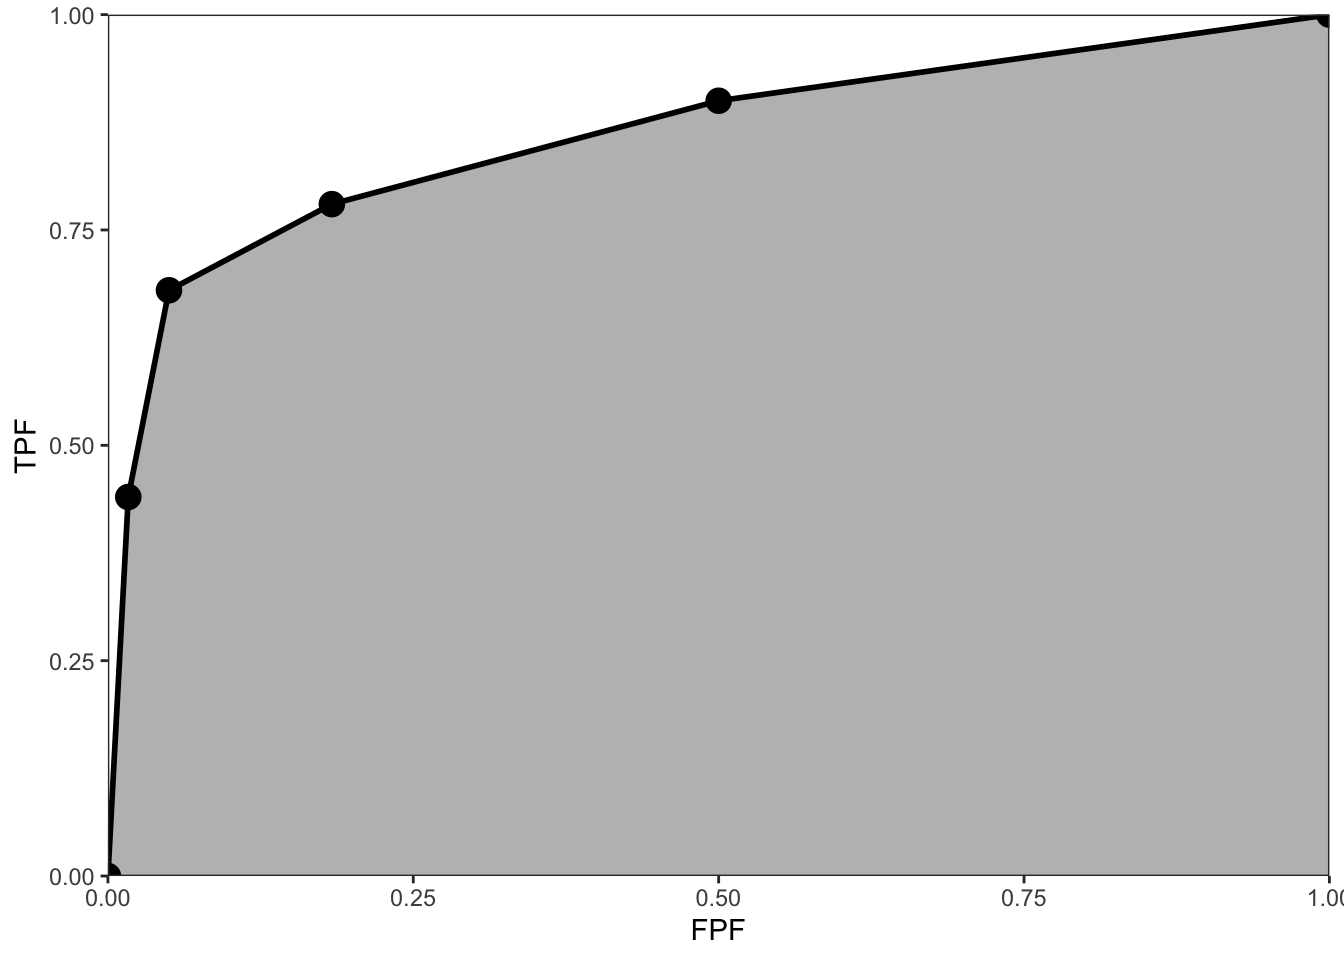
\includegraphics{05-empirical-auc_files/figure-latex/empirical-auc-empirical-auc-1.pdf}
\caption{\label{fig:empirical-auc-empirical-auc}The empirical ROC plot corresponding to Table 4.1; the shaded area is the empirical AUC.}
\end{figure}

\hypertarget{empirical-auc-wilcoxon}{%
\section{The Wilcoxon statistic}\label{empirical-auc-wilcoxon}}

A statistic is any value calculated from observed data. The Wilcoxon statistic is defined by:

\begin{equation}
\text{W}=\frac{1}{K_1K_2} \sum_{k_1=1}^{K_1} \sum_{k_2=1}^{K_2} \psi\left ( z_{k_11} ,  z_{k_22} \right )
\label{eq:empirical-auc-wilcoxon}
\end{equation}

The kernel function \(\psi\left ( x, y \right )\) is defined by:

\begin{equation}
\left.
\begin{aligned}
\psi(x,y)&=1  \qquad & x<y \\
\psi(x,y)&=0.5  & x=y \\
\psi(x,y)&=0  & x>y
\end{aligned}
\right \}
\label{eq:empirical-auc-psi}
\end{equation}

The function \(\psi\left ( x, y \right )\) is unity if the diseased case is rated higher, 0.5 if the two are rated the same and zero otherwise. Each evaluation of the kernel function results from a comparison of a case from the non-diseased set with one from the diseased set. In Eqn. \eqref{eq:empirical-auc-wilcoxon} the two summations and division by the total number of comparisons yields the observed, i.e., empirical, probability that diseased cases are rated higher than non-diseased ones. Since it is a probability, it can range from zero to one. However, if the observer has any discrimination ability at all, one expects diseased cases to be rated equal or greater than non-diseased ones, so in practice one expects \(0.5 \leq \text{W} \leq 1\). The limit 0.5 corresponds to a guessing observer whose operating point lies on the chance diagonal of the ROC plot.

\hypertarget{empirical-auc-wilcoxon-bamber-theorem}{%
\section{Bamber's Equivalence theorem}\label{empirical-auc-wilcoxon-bamber-theorem}}

It is shown in the Appendix \ref{empirical-auc-bamber-theorem-proof} that the Wilcoxon statistic \(\text{W}\) equals the area \(\text{AUC}\) under the empirical ROC plot:

\begin{equation}
\text{W} = \text{AUC}
\label{eq:empirical-auc-bamber-theorem}
\end{equation}

Numerical illustration: as an illustration of the theorem it is helpful to calculate the sum on the right hand side of Eqn. \eqref{eq:empirical-auc-wilcoxon} and compare it to direct integration of the area under the empirical ROC curve (i.e., adding the area of a triangle and several trapezoids). The function is called \texttt{trapz(x,y)}, see below. It takes two array arguments, \(x\) and \(y\), where \(x \equiv \text{FPF}\) and \(y \equiv \text{TPF}\).

\begin{Shaded}
\begin{Highlighting}[]
\NormalTok{trapz }\OtherTok{=} \ControlFlowTok{function}\NormalTok{(x, y)}
\NormalTok{\{ }\DocumentationTok{\#\#\# computes the integral of y with respect to x using trapezoidal integration.}
\NormalTok{  idx }\OtherTok{=} \DecValTok{2}\SpecialCharTok{:}\FunctionTok{length}\NormalTok{(x)}
  \FunctionTok{return}\NormalTok{ (}\FunctionTok{as.double}\NormalTok{( (x[idx] }\SpecialCharTok{{-}}\NormalTok{ x[idx}\DecValTok{{-}1}\NormalTok{]) }\SpecialCharTok{\%*\%}\NormalTok{ (y[idx] }\SpecialCharTok{+}\NormalTok{ y[idx}\DecValTok{{-}1}\NormalTok{])) }\SpecialCharTok{/} \DecValTok{2}\NormalTok{)}
\NormalTok{\}}


\NormalTok{Wilcoxon }\OtherTok{\textless{}{-}} \ControlFlowTok{function}\NormalTok{ (zk1, zk2)}
\NormalTok{\{}
\NormalTok{  K1 }\OtherTok{=} \FunctionTok{length}\NormalTok{(zk1)}
\NormalTok{  K2 }\OtherTok{=} \FunctionTok{length}\NormalTok{(zk2)}
\NormalTok{  W }\OtherTok{\textless{}{-}} \DecValTok{0}
  \ControlFlowTok{for}\NormalTok{ (k1 }\ControlFlowTok{in} \DecValTok{1}\SpecialCharTok{:}\NormalTok{K1) \{}
\NormalTok{    W }\OtherTok{\textless{}{-}}\NormalTok{ W }\SpecialCharTok{+} \FunctionTok{sum}\NormalTok{(zk1[k1] }\SpecialCharTok{\textless{}}\NormalTok{ zk2)}
\NormalTok{    W }\OtherTok{\textless{}{-}}\NormalTok{ W }\SpecialCharTok{+} \FloatTok{0.5} \SpecialCharTok{*} \FunctionTok{sum}\NormalTok{(zk1[k1] }\SpecialCharTok{==}\NormalTok{ zk2)}
\NormalTok{  \}}
\NormalTok{  W }\OtherTok{\textless{}{-}}\NormalTok{ W}\SpecialCharTok{/}\NormalTok{K1}\SpecialCharTok{/}\NormalTok{K2}
  \FunctionTok{return}\NormalTok{ (W)}
\NormalTok{\}}


\NormalTok{RocOperatingPoints }\OtherTok{\textless{}{-}} \ControlFlowTok{function}\NormalTok{( K1, K2 ) \{}
\NormalTok{  nOpPts }\OtherTok{\textless{}{-}} \FunctionTok{length}\NormalTok{(K1) }\SpecialCharTok{{-}} \DecValTok{1} \CommentTok{\# number of op points}
\NormalTok{  FPF }\OtherTok{\textless{}{-}} \FunctionTok{array}\NormalTok{(}\DecValTok{0}\NormalTok{,}\AttributeTok{dim =}\NormalTok{ nOpPts)}
\NormalTok{  TPF }\OtherTok{\textless{}{-}} \FunctionTok{array}\NormalTok{(}\DecValTok{0}\NormalTok{,}\AttributeTok{dim =}\NormalTok{ nOpPts)}
   
  \ControlFlowTok{for}\NormalTok{ (r }\ControlFlowTok{in}\NormalTok{ (nOpPts}\SpecialCharTok{+}\DecValTok{1}\NormalTok{)}\SpecialCharTok{:}\DecValTok{2}\NormalTok{) \{}
\NormalTok{    FPF[r}\DecValTok{{-}1}\NormalTok{] }\OtherTok{\textless{}{-}} \FunctionTok{sum}\NormalTok{(K1[r}\SpecialCharTok{:}\NormalTok{(nOpPts}\SpecialCharTok{+}\DecValTok{1}\NormalTok{)])}\SpecialCharTok{/}\FunctionTok{sum}\NormalTok{(K1)}
\NormalTok{    TPF[r}\DecValTok{{-}1}\NormalTok{] }\OtherTok{\textless{}{-}} \FunctionTok{sum}\NormalTok{(K2[r}\SpecialCharTok{:}\NormalTok{(nOpPts}\SpecialCharTok{+}\DecValTok{1}\NormalTok{)])}\SpecialCharTok{/}\FunctionTok{sum}\NormalTok{(K2)    }
\NormalTok{  \}}
\NormalTok{  FPF }\OtherTok{\textless{}{-}} \FunctionTok{rev}\NormalTok{(FPF)}
\NormalTok{  TPF }\OtherTok{\textless{}{-}} \FunctionTok{rev}\NormalTok{(TPF)}
  
  \FunctionTok{return}\NormalTok{( }\FunctionTok{list}\NormalTok{(}
    \AttributeTok{FPF =}\NormalTok{ FPF,}
    \AttributeTok{TPF =}\NormalTok{ TPF}
\NormalTok{  ) )}
\NormalTok{\}}
\end{Highlighting}
\end{Shaded}

The following code reintroduces the dataset used earlier in Table \ref{tab:ratings-paradigm-example-table}.

\begin{Shaded}
\begin{Highlighting}[]
\NormalTok{RocCountsTable }\OtherTok{=} \FunctionTok{array}\NormalTok{(}\AttributeTok{dim =} \FunctionTok{c}\NormalTok{(}\DecValTok{2}\NormalTok{,}\DecValTok{5}\NormalTok{))}
\NormalTok{RocCountsTable[}\DecValTok{1}\NormalTok{,]  }\OtherTok{\textless{}{-}} \FunctionTok{c}\NormalTok{(}\DecValTok{30}\NormalTok{,}\DecValTok{19}\NormalTok{,}\DecValTok{8}\NormalTok{,}\DecValTok{2}\NormalTok{,}\DecValTok{1}\NormalTok{)}
\NormalTok{RocCountsTable[}\DecValTok{2}\NormalTok{,]  }\OtherTok{\textless{}{-}} \FunctionTok{c}\NormalTok{(}\DecValTok{5}\NormalTok{,}\DecValTok{6}\NormalTok{,}\DecValTok{5}\NormalTok{,}\DecValTok{12}\NormalTok{,}\DecValTok{22}\NormalTok{)}

\NormalTok{zk1  }\OtherTok{\textless{}{-}} \FunctionTok{rep}\NormalTok{(}\DecValTok{1}\SpecialCharTok{:}\FunctionTok{length}\NormalTok{(RocCountsTable[}\DecValTok{1}\NormalTok{,]),RocCountsTable[}\DecValTok{1}\NormalTok{,])}\CommentTok{\#convert frequency table to array}
\NormalTok{zk2  }\OtherTok{\textless{}{-}} \FunctionTok{rep}\NormalTok{(}\DecValTok{1}\SpecialCharTok{:}\FunctionTok{length}\NormalTok{(RocCountsTable[}\DecValTok{2}\NormalTok{,]),RocCountsTable[}\DecValTok{2}\NormalTok{,])}\CommentTok{\#do:}

\NormalTok{w  }\OtherTok{\textless{}{-}} \FunctionTok{Wilcoxon}\NormalTok{ (zk1, zk2)}
\FunctionTok{cat}\NormalTok{(}\StringTok{"The Wilcoxon statistic is = "}\NormalTok{, w, }\StringTok{"}\SpecialCharTok{\textbackslash{}n}\StringTok{"}\NormalTok{)}
\CommentTok{\#\textgreater{} The Wilcoxon statistic is =  0.8606667}
\NormalTok{ret }\OtherTok{\textless{}{-}} \FunctionTok{RocOperatingPoints}\NormalTok{(RocCountsTable[}\DecValTok{1}\NormalTok{,], RocCountsTable[}\DecValTok{2}\NormalTok{,])}
\NormalTok{FPF }\OtherTok{\textless{}{-}}\NormalTok{ ret}\SpecialCharTok{$}\NormalTok{FPF;FPF }\OtherTok{\textless{}{-}} \FunctionTok{c}\NormalTok{(}\DecValTok{0}\NormalTok{,FPF,}\DecValTok{1}\NormalTok{)}
\NormalTok{TPF }\OtherTok{\textless{}{-}}\NormalTok{ ret}\SpecialCharTok{$}\NormalTok{TPF;TPF }\OtherTok{\textless{}{-}} \FunctionTok{c}\NormalTok{(}\DecValTok{0}\NormalTok{,TPF,}\DecValTok{1}\NormalTok{)}
\NormalTok{AUC }\OtherTok{\textless{}{-}} \FunctionTok{trapz}\NormalTok{(FPF,TPF) }\CommentTok{\# trapezoidal integration}
\FunctionTok{cat}\NormalTok{(}\StringTok{"direct integration yields AUC = "}\NormalTok{, AUC, }\StringTok{"}\SpecialCharTok{\textbackslash{}n}\StringTok{"}\NormalTok{)}
\CommentTok{\#\textgreater{} direct integration yields AUC =  0.8606667}
\end{Highlighting}
\end{Shaded}

Note the equality of the two estimates.

\hypertarget{empirical-auc-wilcoxon-bamber-theorem-importance}{%
\section{Importance of Bamber's theorem}\label{empirical-auc-wilcoxon-bamber-theorem-importance}}

The equivalence theorem is the starting point for all non-parametric methods of analyzing ROC plots, e.g., \citep{hanley1997sampling, delong1988comparing}. Prior to Bamber's work one knew how to plot an empirical operating characteristic and how to calculate the Wilcoxon statistic, but their equality had not been shown. This was Bamber's essential contribution. In the absence of this theorem, the Wilcoxon statistic would be ``just another statistic'', at least in the context of ROC analysis. The theorem is so important that a paper appeared in Radiology \citep{hanley1982meaning} devoted to the equivalence. The title of this paper was ``The meaning and use of the area under a receiver operating characteristic (ROC) curve''. The equivalence theorem literally gives meaning to the empirical area under the ROC.

\hypertarget{empirical-auc-discussion-summary}{%
\section{Discussion / Summary}\label{empirical-auc-discussion-summary}}

In this chapter, a simple method for estimating the empirical area under the ROC plot has been described. Its simplicity and clear physical interpretation as the AUC under the empirical ROC (not fitted, not true) has spurred much theoretical development. Since the empirical AUC always yields a number the researcher could be unaware about unusual behavior of the empirical ROC curve, so it is a good idea to plot the data and look for any signs of large extrapolations. An example would be data points clustered at low \(\text{FPF}\) values, which imply a large AUC contribution, unsupported by intermediate operating points, from the line connecting the uppermost non-trivial operating point to (1,1).

\hypertarget{empirical-auc-bamber-theorem-proof}{%
\section{Appendix: Bamber theorem proof}\label{empirical-auc-bamber-theorem-proof}}

The following proof is adapted from \citep{bamber1975area} and while it may appear to be restricted to discrete ratings, the result is in fact quite general, i.e., it is applicable even if the ratings are acquired on a continuous scale. The reason is that in an R-rating ROC study the observed z-samples or ratings take on integer values, 1 through R. If R is large enough, ordering information present in the continuous data is not lost upon binning. In the following it is helpful to keep in mind that one is dealing with discrete distributions of the ratings, described by probability mass functions as opposed to probability density functions, e.g., \(P(Z_2 = \zeta_i)\) is not zero, as would be the case for continuous ratings. The proof is illustrated with Fig. \ref{fig:empirical-auc-bamber-theorem}.

\begin{figure}
\centering
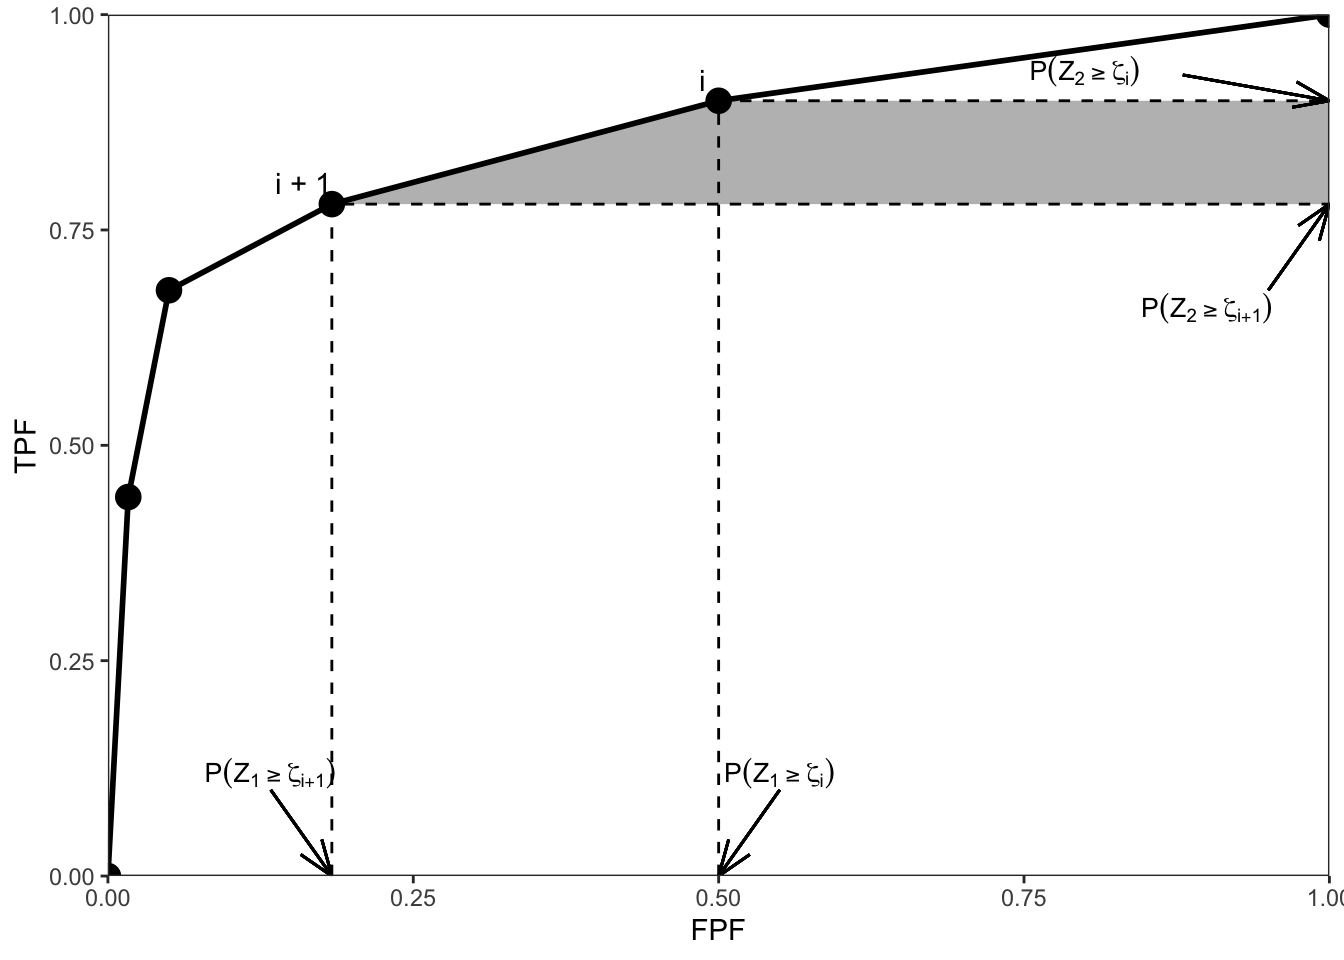
\includegraphics{05-empirical-auc_files/figure-latex/empirical-auc-bamber-theorem-1.pdf}
\caption{\label{fig:empirical-auc-bamber-theorem}:Illustration of the derivation of Bamber's equivalence theorem. Shows an empirical ROC plot for R = 5; the shaded area is due to points labeled i and i + 1.}
\end{figure}

The abscissa of the operating point \(i\) is \(P(Z_1 \geq \zeta_i)\) and the corresponding ordinate is \(P(Z_2 \geq \zeta_i)\). Here \(Z_1\) is a random sample from a non-diseased case and \(Z_2\) is a random sample from a diseased case. The shaded trapezoid defined by drawing horizontal lines from operating points \(i\) (upper) and \(i+1\) (lower) to the right edge of the ROC plot, Fig. \ref{fig:empirical-auc-bamber-theorem}, has height:

\begin{equation}
P\left ( Z_2 \geq \zeta_i \right ) - P\left ( Z_2 \geq \zeta_{i+1} \right ) = P\left ( Z_2 = \zeta_i \right )
\label{eq:empirical-auc-bamber-theorem-proof1}
\end{equation}

The validity of this equation can perhaps be more easily seen when the first term is written in the form:

\begin{equation}
P\left ( Z_2 \geq \zeta_i \right ) = P\left ( Z_2 = \zeta_i \right )  + P\left ( Z_2 \geq \zeta_{i+1} \right )
\label{eq:empirical-auc-bamber-theorem-proof2}
\end{equation}

The lengths of the top and bottom edges of the trapezoid are, respectively:

\begin{equation}
1-P\left ( Z_1 \geq \zeta_i \right )=P\left ( Z_1 < \zeta_i \right )
\label{eq:empirical-auc-bamber-theorem-proof3}
\end{equation}

and

\begin{equation}
1-P\left ( Z_1 \geq \zeta_{i+1} \right )=P\left ( Z_1 < \zeta_{i+1} \right )
\label{eq:empirical-auc-bamber-theorem-proof4}
\end{equation}

The area \(A_i\) of the shaded trapezoid in Fig. \ref{fig:empirical-auc-bamber-theorem} is (the steps are shown explicitly):

\begin{equation}
\left.
\begin{aligned}
A_i &=\frac{1}{2}P\left ( Z_2 = \zeta_i \right )\left [ P\left ( Z_1 < \zeta_i \right ) +  P\left ( Z_1 < \zeta_{i+1} \right ) \right ] \\
A_i &=P\left ( Z_2 = \zeta_i \right )\left [ \frac{1}{2}P\left ( Z_1 < \zeta_i \right ) +  \frac{1}{2} \left (P\left ( Z_1 = \zeta_i \right ) + P\left ( Z_1 < \zeta_i \right ) \right ) \right ]\\
A_i &=P\left ( Z_2 = \zeta_i \right )\left [ \frac{1}{2} P\left ( Z_1 = \zeta_i \right ) +  P\left ( Z_1 < \zeta_i \right ) \right ] \\
\end{aligned}
\right \}
\label{eq:empirical-auc-bamber-theorem-proof5}
\end{equation}

Summing over all values of \(i\), one gets for the total area under the empirical ROC plot:

\begin{equation}
\left.
\begin{aligned}
AUC & = \sum_{i=0}^{R-1}A_i\\
 & = \frac{1}{2}\sum_{i=0}^{R-1}P\left ( Z_2=\zeta_i \right )P\left ( Z_1=\zeta_i \right )+\sum_{i=0}^{R-1}P\left ( Z_2=\zeta_i \right )P\left ( Z_1<\zeta_i \right )
\end{aligned}
\right \}
\label{eq:empirical-auc-bamber-theorem-proof6}
\end{equation}

It is shown in \ref{empirical-auc-bamber-theorem-a0-term} that the term \(A_0\) corresponds to the triangle at the upper right corner of Fig. \ref{fig:empirical-auc-bamber-theorem}, and the term \(A_4\) corresponds to the horizontal trapezoid defined by the lowest non-trivial operating point.

Eqn. \eqref{eq:empirical-auc-bamber-theorem-proof6} can be restated as:

\begin{equation}
AUC=\frac{1}{2}P\left ( Z_1 = Z_2 \right ) + P\left ( Z_1 < Z_2 \right )
\label{eq:empirical-auc-bamber-theorem-proof7}
\end{equation}

The Wilcoxon statistic was defined in Eqn. \eqref{eq:empirical-auc-wilcoxon}. It can be seen that the comparisons implied by the summations and the weighting implied by the kernel function are estimating the two probabilities in the expression for in Eqn. \eqref{eq:empirical-auc-bamber-theorem-proof7}. Therefore, \(AUC = W\).

\hypertarget{empirical-auc-bamber-theorem-a0-term}{%
\section{\texorpdfstring{Appendix: The \(A_0\) term}{Appendix: The A\_0 term}}\label{empirical-auc-bamber-theorem-a0-term}}

\hypertarget{upper-triangle}{%
\subsection{Upper triangle}\label{upper-triangle}}

For \(i = 0\), Eqn. \eqref{eq:empirical-auc-bamber-theorem-proof5} implies (since the lowest empirical threshold is unity, the lowest allowed rating, and there are no cases rated less than one):

\begin{equation}
\left. 
\begin{aligned}
A_0 =& P\left ( Z_2 = 1 \right )\left [ \frac{1}{2} P\left ( Z_1=1 \right ) + P\left ( Z_1<1 \right )\right ] \\
A_0 =& \frac{1}{2} P\left ( Z_1=1 \right ) P\left ( Z_2=1 \right )\\
\end{aligned}
\right \}
\end{equation}

The base of the triangle is:

\begin{equation}
1 - P\left ( Z_1 \geq 2 \right )=P\left ( Z_1 < 2 \right )=P\left ( Z_1 = 1 \right )
\end{equation}

The height of the triangle is:

\begin{equation}
1 - P\left ( Z_2 \geq 2 \right )=P\left ( Z_2 < 2 \right )=P\left ( Z_2 = 1 \right )
\end{equation}

Q.E.D.

\hypertarget{lowest-trapezoid}{%
\subsection{Lowest trapezoid}\label{lowest-trapezoid}}

For \(i = 4\), Eqn. \eqref{eq:empirical-auc-bamber-theorem-proof5} implies:

\begin{equation}
\left.
\begin{aligned}
A_4 =& P\left ( Z_2=5 \right )\left [ \frac{1}{2}P\left ( Z_1=5 \right ) + P\left ( Z_1<5 \right )\right ] \\
A_4 =& \frac{1}{2}P\left ( Z_2=5 \right )\left [ P\left ( Z_1=5 \right ) + 2P\left ( Z_1<5 \right )\right ] \\
A_4 =& \frac{1}{2}P\left ( Z_2=5 \right )\left [ P\left ( Z_1=5 \right ) +P\left ( Z_1<5 \right ) + P\left ( Z_1<5 \right )\right ] \\
A_4 =& \frac{1}{2}P\left ( Z_2=5 \right )\left [ 1 + P\left ( Z_1<5 \right )\right ] \\
\end{aligned}
\right \}
\end{equation}

The upper side of the trapezoid is

\begin{equation}
1-P\left ( Z_1 \geq 5 \right )= P\left ( Z_1 < 5 \right )
\end{equation}

The lower side is unity. The average of the two sides is:

\begin{equation}
\frac{1 + P\left ( Z_1 < 5 \right )}{2}
\end{equation}

The height is:

\begin{equation}
P\left ( Z_2 \geq 5 \right ) = P\left ( Z_2 = 5 \right )
\end{equation}

Multiplication of the last two expressions yields \(A_4\).

\hypertarget{empirical-auc-references}{%
\section{Chapter References}\label{empirical-auc-references}}

\hypertarget{binormal-model}{%
\chapter{Binormal model}\label{binormal-model}}

\hypertarget{binormal-model-how-much-finished}\label{binormal-model-how-much-finished}}

\hypertarget{binormal-model-introduction}{%
\section{Introduction}\label{binormal-model-introduction}}

The equal variance binormal model was described in Chapter \ref{binary-task}. The ratings method of acquiring ROC data and calculation of operating points was discussed in Chapter \ref{ratings-paradigm}. It was shown there that for a clinical dataset the unequal-variance binormal model visually fitted the data better than the equal-variance binormal model.

This chapter deals with the unequal-variance binormal model, often abbreviated to \textbf{binormal model}. It is applicable to univariate datasets in which there is \emph{one rating per case}, as in a single observer interpreting cases, one at a time, in a single modality. By convention the qualifier ``univariate'' is often omitted. In Chapter \texttt{TempComment\ \textbackslash{}@ref(bivariate-binormal-model)} a bivariate model will be described where each case yields two ratings, as in a single observer interpreting cases in two modalities, or the similar problem of two observers interpreting the same cases in a single modality.

\hypertarget{binormal-model-definition}{%
\section{Binormal model}\label{binormal-model-definition}}

The binormal model is defined by (capital letters indicate random variables lower-case are realized values and \(t\) denotes the truth state):

\begin{equation} 
\left.
\begin{aligned}
Z_{k_tt} \sim &N\left ( \mu_t,\sigma_{t}^{2} \right )\\
t&=1,2
\end{aligned}
\right \}
\label{eq:binormal-model-z-samples-1}
\end{equation}

where

\begin{equation} 
\left.
\begin{aligned}
\mu_1=&0\\
\mu_2=&\mu\\
\sigma_{1}^{2}=&1\\
\sigma_{2}^{2}=&\sigma^{2}
\end{aligned}
\right \}
\label{eq:binormal-model-z-samples-2}
\end{equation}

Eqn. \eqref{eq:binormal-model-z-samples-1} states that the z-samples for non-diseased cases (\(t = 1\)) are distributed as a \(N(0,1)\) distribution, i.e., the unit normal distribution, while the z-samples for diseased cases (\(t = 2\)) are distributed as a \(N(\mu,\sigma^2)\) distribution, i.e., a normal distribution with mean \(\mu\) and variance \(\sigma^2\). In the unequal-variance binormal model, the variance \(\sigma^2\) of the z-samples for diseased cases is allowed to be different from unity. Most ROC datasets are consistent with \(\sigma > 1\).\footnote{A more complicated version of this model would allow the mean of the non-diseased distribution to be non-zero and its variance different from unity. The resulting 4-parameter model is no more general than the 2-parameter model. The reason is that one is free to transform the decision variable, and associated thresholds, by applying arbitrary monotonic increasing function transformation, which do not change the ordering of the ratings and hence do not change the ROC curve. So if the mean of the noise distribution were non-zero, subtracting this value from all Z-samples would shift the effective mean of the non-diseased distribution to zero (the shifted Z-values are monotonically related to the original values) and the mean of the shifted diseased distribution becomes \(\mu_2-\mu_1\). Next, one scales or divides (division by a positive number is also a monotonic transformation) all the Z-samples by \(\sigma_1\), resulting in the scaled non-diseased distribution having unit variance, and the scaled diseased distribution has mean \(\frac{\mu_2-\mu_1}{\sigma_1}\) and variance \((\frac{\sigma_2}{\sigma_1})^2\). Therefore, if one starts with 4 parameters then one can, by simple shifting and scaling operations, reduce the model to 2 parameters, as in Eqn. \eqref{eq:binormal-model-z-samples-1}.}

\hypertarget{binned-data}{%
\subsection{Binned data}\label{binned-data}}

In an R-rating ROC study the observed ratings \(r\) take on integer values 1 through \(R\) it being understood that higher ratings correspond to greater confidence for presence of disease. Define \(R-1\) ordered cutoffs \(\zeta_i\) where \(i=1,2,...,R-1\) and \(\zeta_1 < \zeta_2,...< \zeta_{R-1}\). Also define two dummy cutoffs \(\zeta_0 = -\infty\) and \(\zeta_R = +\infty\). The \textbf{binning rule} for a case with realized z-sample z is (Chapter \ref{ratings-paradigm}, Eqn. \eqref{eq:ratings-paradigm-binning-rule}):

\begin{equation}
\left.
\begin{aligned}  
\text{if} \left (\zeta_{r-1} \le z < \zeta_r  \right )&\Rightarrow \text{rating} = r\\
&r = 1, 2, ..., R
\end{aligned}
\right \}
\label{eq:binormal-model-binning-rule}
\end{equation}

\begin{figure}
\centering
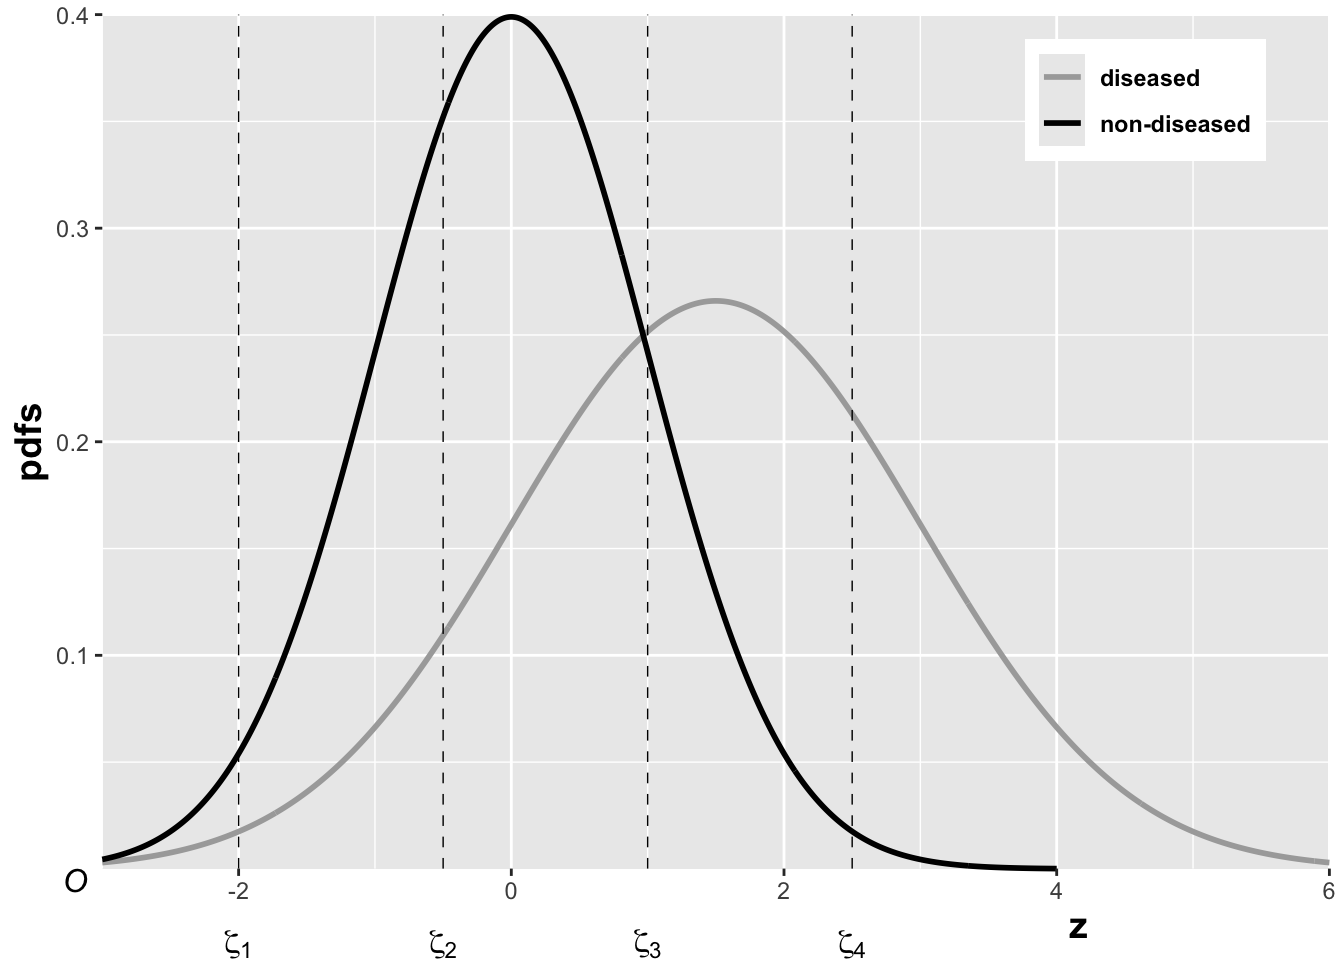
\includegraphics{06-binormal-model_files/figure-latex/binormal-model-pdfs-1.pdf}
\caption{\label{fig:binormal-model-pdfs}The pdfs of the two binormal model distributions for \(\mu = 1.5\) and \(\sigma = 1.5\). Four thresholds \(\zeta_1, \zeta_2, \zeta_3, \zeta_4\) are shown corresponding to a five-rating ROC study. The rating assigned to a case is determined by its z-sample according to the binning rule.}
\end{figure}

The above figure, generated with \(\mu = 1.5\), \(\sigma = 1.5\), \(\zeta_1 = -2\), \(\zeta_2 = -0.5\), \(\zeta_3 = 1\) and \(\zeta_4 = 2.5\), illustrates how realized z-samples are converted to ratings, i.e., application of the binning rule \eqref{eq:binormal-model-binning-rule}. For example, a case with z-sample equal to -2.5 would be rated ``1'', and one with z-sample equal to -1 would be rated ``2'', cases with z-samples greater than 2.5 would be rated ``5''.

\hypertarget{sensitivity-and-specificity-1}{%
\subsection{Sensitivity and specificity}\label{sensitivity-and-specificity-1}}

Let \(Z_t\) denote the random z-sample for truth state \(t\) (\(t\) = 1 for non-diseased and \(t\) = 2 for diseased cases). Since the distribution of z-samples from disease-free cases is \(N(0,1)\), the expression for specificity in Chapter \ref{binary-task-model} applies:

\begin{equation} 
\text{Sp}\left ( \zeta \right )=P\left ( Z_1 < \zeta \right )=\Phi\left ( \zeta \right )
\label{eq:binormal-model-specificity}
\end{equation}

To obtain an expression for sensitivity, consider that for truth state \(t = 2\), the random variable \(\frac{Z_2-\mu}{\sigma}\) is distributed as \(N(0,1)\):

\begin{equation*} 
\frac{Z_2-\mu}{\sigma}\sim N\left ( 0,1 \right )
\end{equation*}

Sensitivity, abbreviated to \(\text{Se}\), is defined by \(\text{Se} \equiv P\left ( Z_2 > \zeta \right )\). It follows, because \(\sigma\) is positive, that:

\begin{equation*} 
\text{Se}\left ( \zeta | \mu, \sigma \right ) = P\left ( \frac{Z_2-\mu}{\sigma} > \frac{\zeta-\mu}{\sigma} \right )
\end{equation*}

The right-hand-side can be rewritten as follows:

\begin{equation} 
\left. 
\begin{aligned}
\text{Se}\left ( \zeta | \mu, \sigma \right )&= 1 - P\left ( \frac{Z_2-\mu}{\sigma} \leq  \frac{\zeta-\mu}{\sigma} \right )\\
&=1-\Phi\left (  \frac{\zeta-\mu}{\sigma}\right )=\Phi\left (  \frac{\mu-\zeta}{\sigma}\right )
\end{aligned}
\right \}
\label{eq:binormal-model-sensitivity2}
\end{equation}

Summarizing, the formulae for the specificity and sensitivity for the binormal model are:

\begin{equation} 
\left. 
\begin{aligned}
\text{Sp}\left ( \zeta \right ) &= \Phi\left ( \zeta \right )\\
\text{Se}\left ( \zeta | \mu, \sigma \right ) &= \Phi\left (  \frac{\mu-\zeta}{\sigma}\right )
\end{aligned}
\right \}
\label{eq:binormal-model-se-sp}
\end{equation}

The coordinates of the operating point defined by \(\zeta\) are given by:

\begin{equation} 
\left. 
\begin{aligned}
\text{FPF}\left ( \zeta \right ) &= 1 - \text{Sp}\left ( \zeta \right ) \\
&= 1 - \Phi\left ( \zeta \right ) \\
&= \Phi\left ( -\zeta \right )
\end{aligned}
\right \}
\label{eq:binormal-model-fpf}
\end{equation}

\begin{equation} 
\text{TPF}\left ( \zeta | \mu, \sigma \right ) = \Phi\left ( \frac{\mu-\zeta}{\sigma} \right )
\label{eq:binormal-model-tpf}
\end{equation}

An equation for a curve is usually expressed as \(y=f(x)\). An expression of this form for the ROC curve, i.e., the y-coordinate (TPF) expressed as a function of the x-coordinate (FPF), follows upon inversion of the expression for FPF, Eqn. \eqref{eq:binormal-model-fpf}:

\begin{equation} 
\zeta = -\Phi^{-1}\left ( \text{FPF} \right )
\label{eq:binormal-model-zeta}
\end{equation}

Substitution of Eqn. \eqref{eq:binormal-model-zeta} in Eqn. \eqref{eq:binormal-model-tpf} yields:

\begin{equation} 
\text{TPF} = \Phi\left ( \frac{\mu + \Phi^{-1}\left (\text{FPF}  \right )}{\sigma} \right )
\label{eq:binormal-model-roc-curve1}
\end{equation}

This equation will be put into conventional notation next.

\hypertarget{binormal-model-in-conventional-notation}{%
\subsection{Binormal model in conventional notation}\label{binormal-model-in-conventional-notation}}

The \((\mu,\sigma)\) notation just described makes sense when extending the binormal model to newer models described later (see Chapter \texttt{TempComment\ \textbackslash{}@ref(proper-roc-models)}). However, it was not the way the binormal model was originally parameterized. Instead the following notation is widely used in the literature:

\begin{equation} 
\left. 
\begin{aligned}
a&=\frac{\mu}{\sigma}\\
b&=\frac{1}{\sigma}
\end{aligned}
\right \}
\label{eq:binormal-model-ab-parameters}
\end{equation}

\begin{quote}
The reason for the \((a,b)\) instead of the \((\mu,\sigma)\) notation is historical. \citep{dorfman1969maximum} assumed that the diseased distribution had unit variance, and the non-diseased distribution had standard deviation \(b\) and their separation was \(a\), see Plot A in Fig. \ref{fig:binormal-model-ab2-mu-sigma}.
\end{quote}

By dividing the z-samples by \(b\), the variance of the distribution labeled ``Noise'' becomes unity, its mean stays at zero, and the variance of the distribution labeled ``Signal'' becomes \(1/b\), and its mean becomes \(a/b\), see plot B. Accordingly the inverses of Eqn. \eqref{eq:binormal-model-ab-parameters} are:

\begin{equation} 
\left. 
\begin{aligned}
\mu&=\frac{a}{b}\\
\sigma&=\frac{1}{b}
\end{aligned}
\right \}
\label{eq:binormal-model-ab-parameters-inv}
\end{equation}

Eqns. \eqref{eq:binormal-model-ab-parameters} and \eqref{eq:binormal-model-ab-parameters-inv} allow conversion from one notation to another.

\begin{figure}
\centering
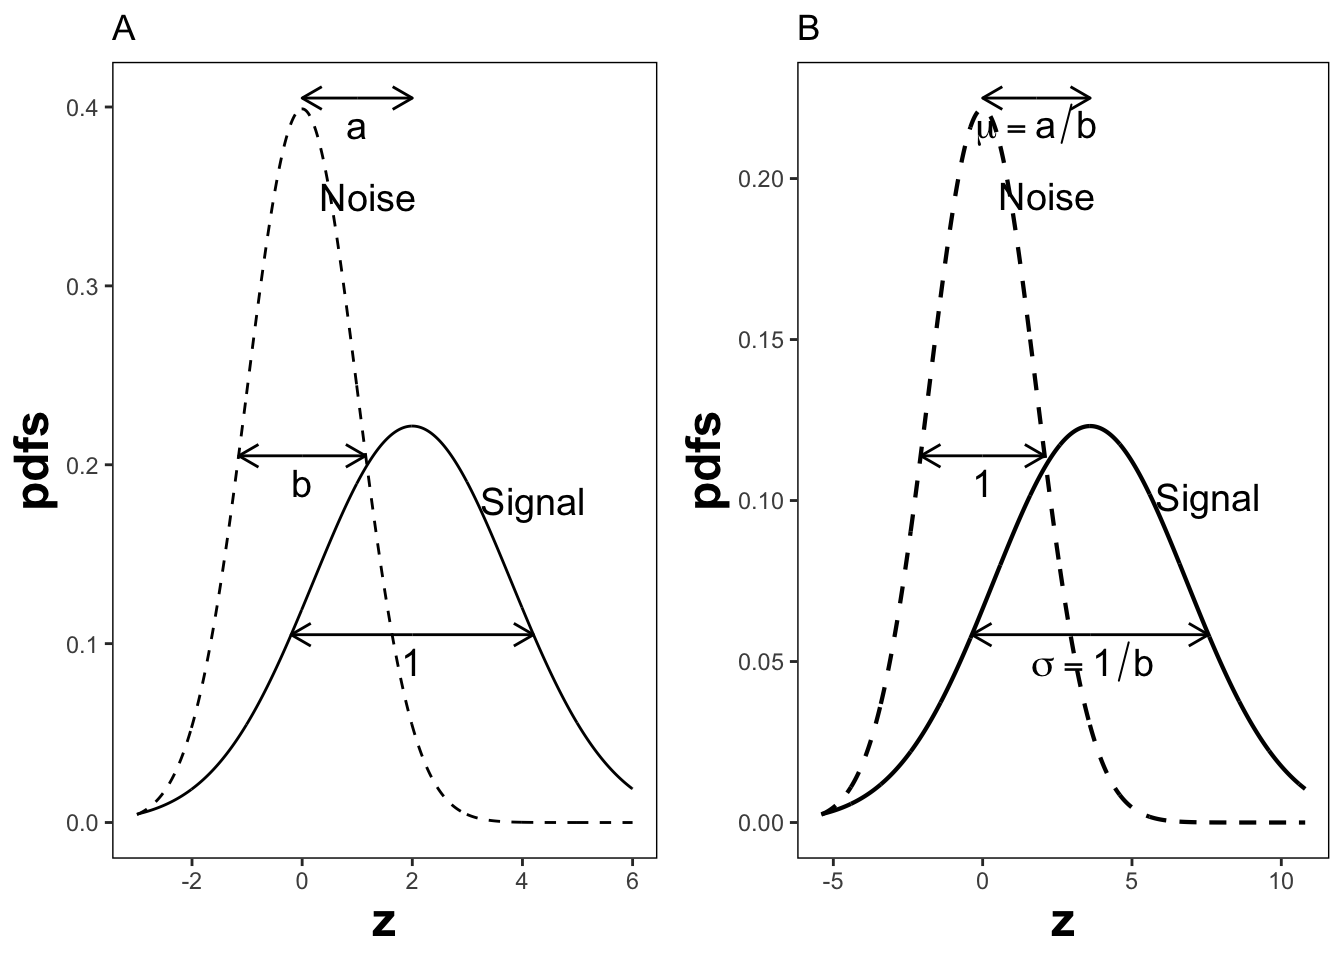
\includegraphics{06-binormal-model_files/figure-latex/binormal-model-ab2-mu-sigma-1.pdf}
\caption{\label{fig:binormal-model-ab2-mu-sigma}Plot A shows the definitions of the (a,b) parameters of the binormal model. In plot B the x-axis has been rescaled so that the noise distribution has unit variance; this illustrates the difference between the (a,b) and the (\(\mu,\sigma\)) parameters. In this figure \(\mu = 2\) and \(\sigma = 1.8\) which correspond to \(a = 1.11\) and \(b = 0.556\).}
\end{figure}

\hypertarget{binormal-model-roc-curve}{%
\section{ROC curve}\label{binormal-model-roc-curve}}

Using the \((a,b)\) notation, Eqn. \eqref{eq:binormal-model-roc-curve1} for the ROC curve reduces to:

\begin{equation} 
\text{TPF}\left ( \text{FPF} \right ) = \Phi\left ( a+ b \Phi^{-1}\left (\text{FPF}  \right ) \right )
\label{eq:binormal-model-roc-curve-tpf-fpf}
\end{equation}

Since \(\Phi^{-1}(\text{FPF})\) is an increasing function of its argument \(\text{FPF}\), and \(b > 0\), the argument of the \(\Phi\) function is an increasing function of \(\text{FPF}\). Since \(\Phi\) is a monotonically increasing function of its argument, \(\text{TPF}\) is a monotonically increasing function of \(\text{FPF}\). This is true regardless of the sign of \(a\). If \(\text{FPF} = 0\), then \(\Phi^{-1}(0) = -\infty\) and \(\text{TPF} = 0\). If \(\text{FPF} = 1\), then \(\Phi^{-1}(1) = +\infty\) and \(\text{TPF} = 1\). Regardless of the value of \(a\), as long as \(b \ge 0\), the ROC curve starts at (0,0) and increases monotonically to (1,1).

From Eqn. \eqref{eq:binormal-model-fpf} and Eqn. \eqref{eq:binormal-model-tpf}, the expressions for \(\text{FPF}\) and \(\text{TPF}\) in terms of model parameters \((a,b)\) are:

\begin{equation}
\left.
\begin{aligned}
\text{FPF}\left ( \zeta \right ) &= \Phi\left ( -\zeta \right )\\
\text{TPF}\left (\zeta | a,b \right ) &= \Phi\left ( a - b \zeta \right )
\end{aligned}
\right \}
\label{eq:binormal-model-op-point-ab}
\end{equation}

Solve for \(\zeta\) from the equation for FPF:

\begin{equation}
\zeta = - \Phi^{-1}\left ( \text{FPF} \right )
\label{eq:binormal-model-op-point-ab1}
\end{equation}

\hypertarget{binormal-model-pdfs}{%
\section{Density functions}\label{binormal-model-pdfs}}

According to Eqn. \eqref{eq:binormal-model-z-samples-1} the probability that a non-diseased case z-sample is smaller than \(\zeta\), i.e., the cumulative distribution function (CDF) function for non-diseased cases, is:

\begin{equation*} 
P\left ( Z \le \zeta \mid  Z\sim N\left ( 0,1 \right ) \right ) = 1-FPF\left ( \zeta \right ) = \Phi \left ( \zeta  \right )
\end{equation*}

Likewise, the CDF for diseased case z-samples is:

\begin{equation*} 
P\left ( Z \le \zeta \mid  Z\sim N\left ( \mu,\sigma^2 \right ) \right ) = 1-\text{TPF}\left ( \zeta \right ) = \Phi \left ( \frac{\zeta - \mu}{\sigma}  \right )
\end{equation*}

Since the \emph{pdf} is the derivative of the corresponding CDF function, it follows that (the superscripts N and D denote non-diseased and diseased cases, respectively):

\begin{equation} 
\left.
\begin{aligned}
pdf_N\left ( \zeta \right ) &= \frac{\partial \Phi\left ( \zeta \right )}{\partial \zeta} \\
&= \phi\left ( \zeta \right ) \\
&\equiv \frac{1}{\sqrt{2 \pi}}\exp\left ( -\frac{\zeta^2}{2} \right )
\end{aligned}
\right \}
\label{eq:binormal-model-pdf-n}
\end{equation}

\begin{equation} 
\left.
\begin{aligned}
pdf_D\left ( \zeta \right ) &= \frac{\partial \Phi\left ( \frac{\zeta - \mu}{\sigma} \right )}{\partial \zeta} \\ &= \frac{1}{\sigma} \phi\left ( \frac{\zeta - \mu}{\sigma} \right ) \\
&\equiv \frac{1}{\sqrt{2 \pi}\sigma}\exp\left ( -\frac{\left (\zeta-\mu  \right )^2}{2\sigma} \right )
\end{aligned}
\right \}
\label{eq:binormal-model-pdf-d-mu-sigma}
\end{equation}

The second equation can be written in \((a,b)\) notation as:

\begin{equation} 
\left.
\begin{aligned}
pdf_D\left ( \zeta \right ) &= b\phi\left ( b\zeta-a \right ) \\
&= \frac{b}{\sqrt{2 \pi}}\exp\left ( -\frac{\left (b\zeta - a \right )^2}{2} \right )
\end{aligned}
\right \}
\label{eq:binormal-model-pdf-d-a-b}
\end{equation}

\hypertarget{binormal-model-invariance-property}{%
\section{Invariance property of pdfs}\label{binormal-model-invariance-property}}

The binormal model is not as restrictive as might appear at first sight. Any monotone increasing transformation \(Y=f(Z)\) applied to the observed z-samples, and the associated thresholds, will yield the same observed data, e.g., Table \ref{tab:ratings-paradigm-example-table}. This is because such a transformation leaves the ordering of the ratings unaltered and hence results in the same operating points. While the distributions for \(Y\) will not be binormal (i.e., two independent normal distributions), one can safely ``pretend'' that one is still dealing with an underlying binormal model. An alternative way of stating this is that any pair of distributions is allowed as long as they are reducible to a binormal model form by a monotonic increasing transformation of Y: e.g., \(Z=f^{-1}\). {[}If \(f\) is a monotone increasing function of its argument, so is \(f^{-1}\)\}.{]} For this reason, the term ``pair of latent underlying normal distributions'' is sometimes used to describe the binormal model. The robustness of the binormal model has been investigated \citep{hanley1988robustness, dorfman1997proper}. The referenced paper by Dorfman et al has an excellent discussion of the robustness of the binormal model.

The robustness of the binormal model, i.e., the flexibility allowed by the infinite choices of monotonic increasing functions, application of each of which leaves the ordering of the data unaltered, is widely misunderstood. The non-Gaussian appearance of histograms of ratings in ROC studies can lead one to incorrect conclusions that the binormal model is inapplicable to these datasets. To quote a reviewer of one of my recent papers:

\begin{quote}
I have had multiple encounters with statisticians who do not understand this difference\ldots. They show me histograms of data, and tell me that the data is obviously not normal, therefore the binormal model should not be used.
\end{quote}

The reviewer is correct. The misconception is illustrated next.

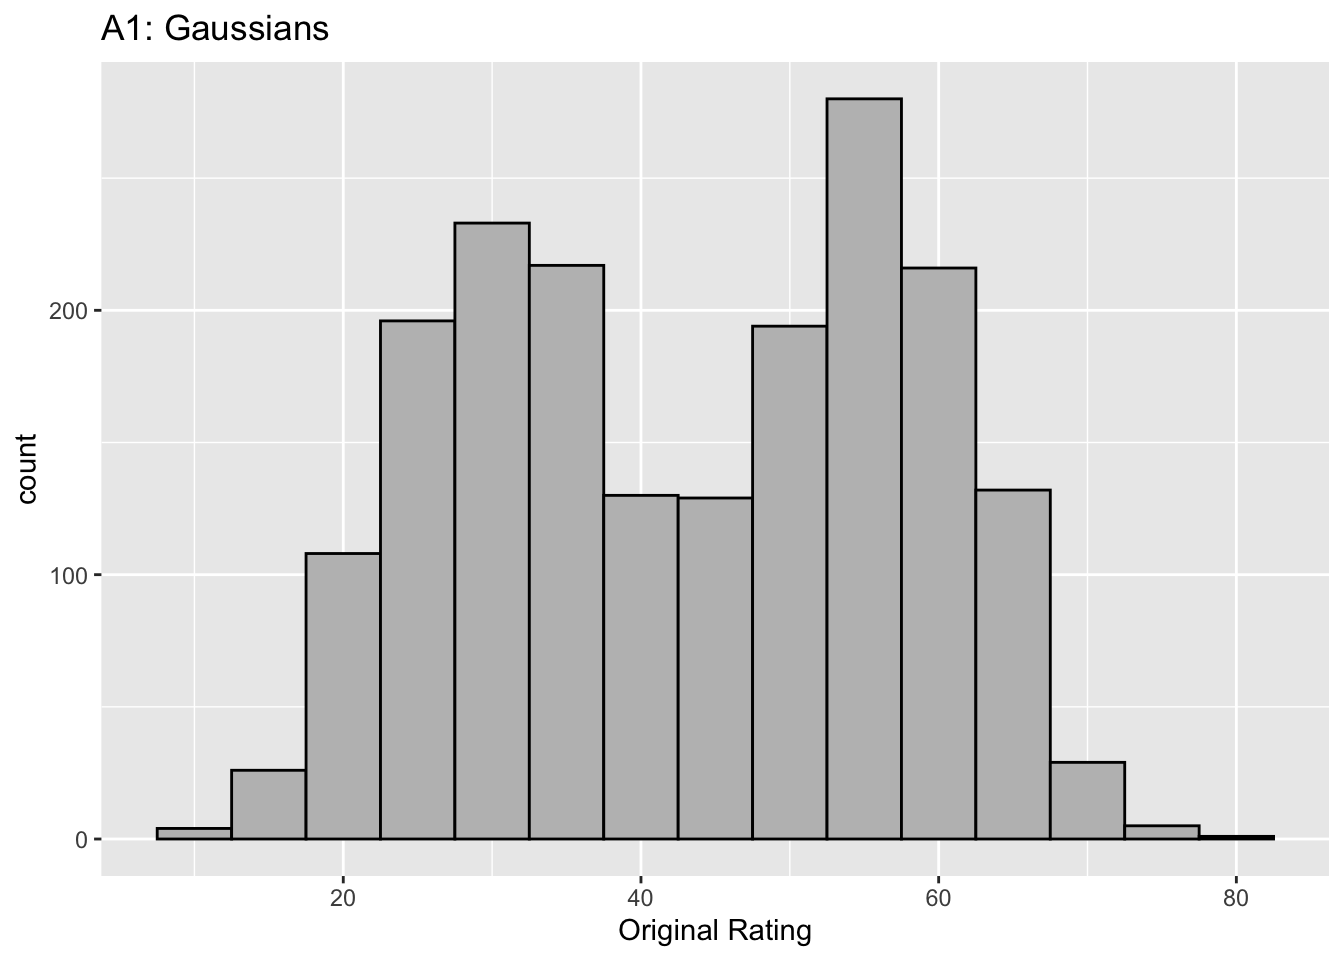
\includegraphics[width=0.33\linewidth]{06-binormal-model_files/figure-latex/unnamed-chunk-6-1} 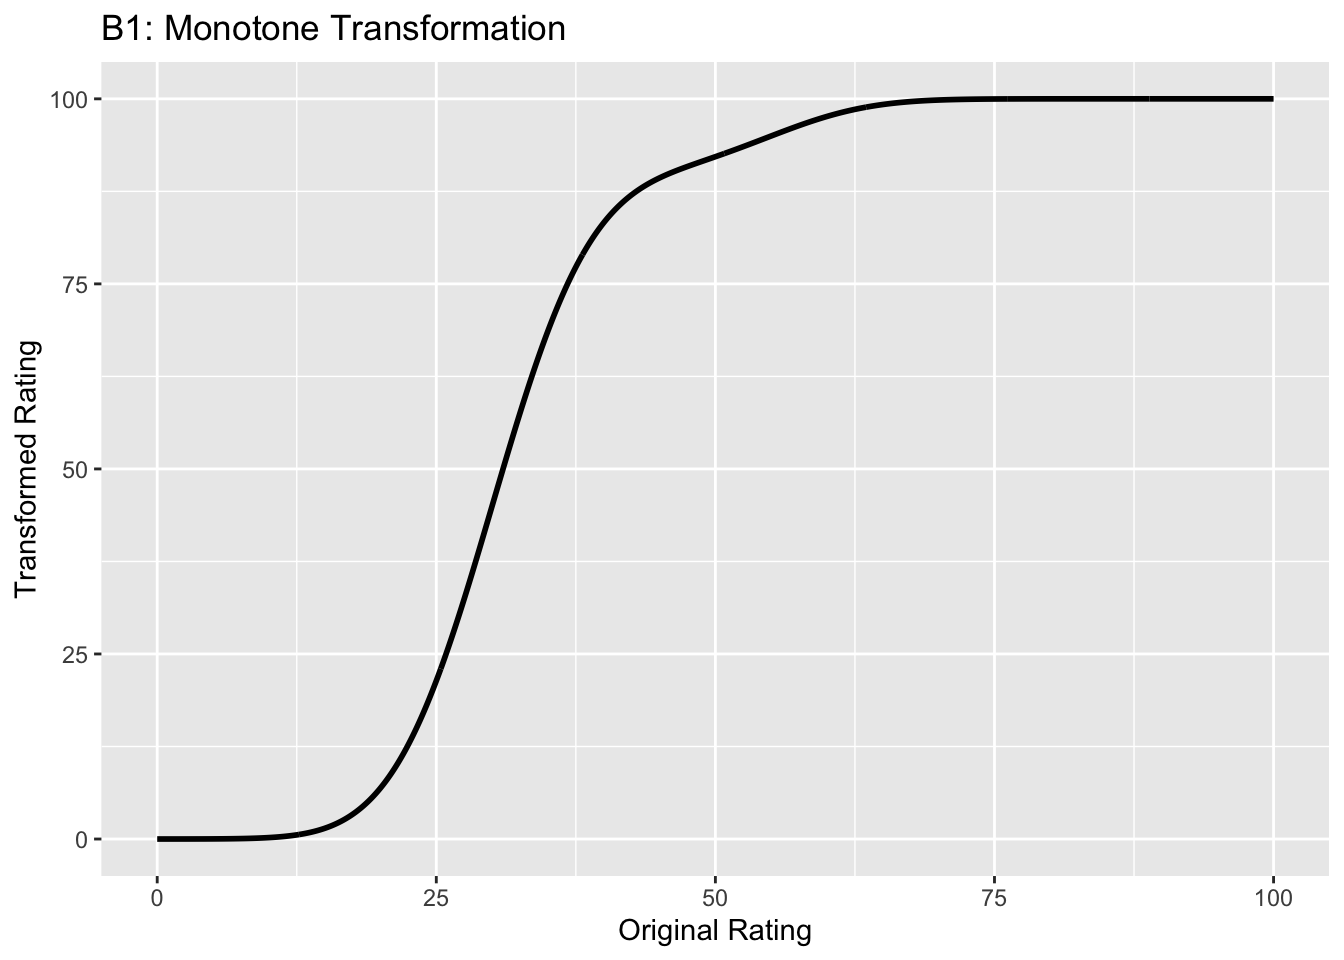
\includegraphics[width=0.33\linewidth]{06-binormal-model_files/figure-latex/unnamed-chunk-6-2} 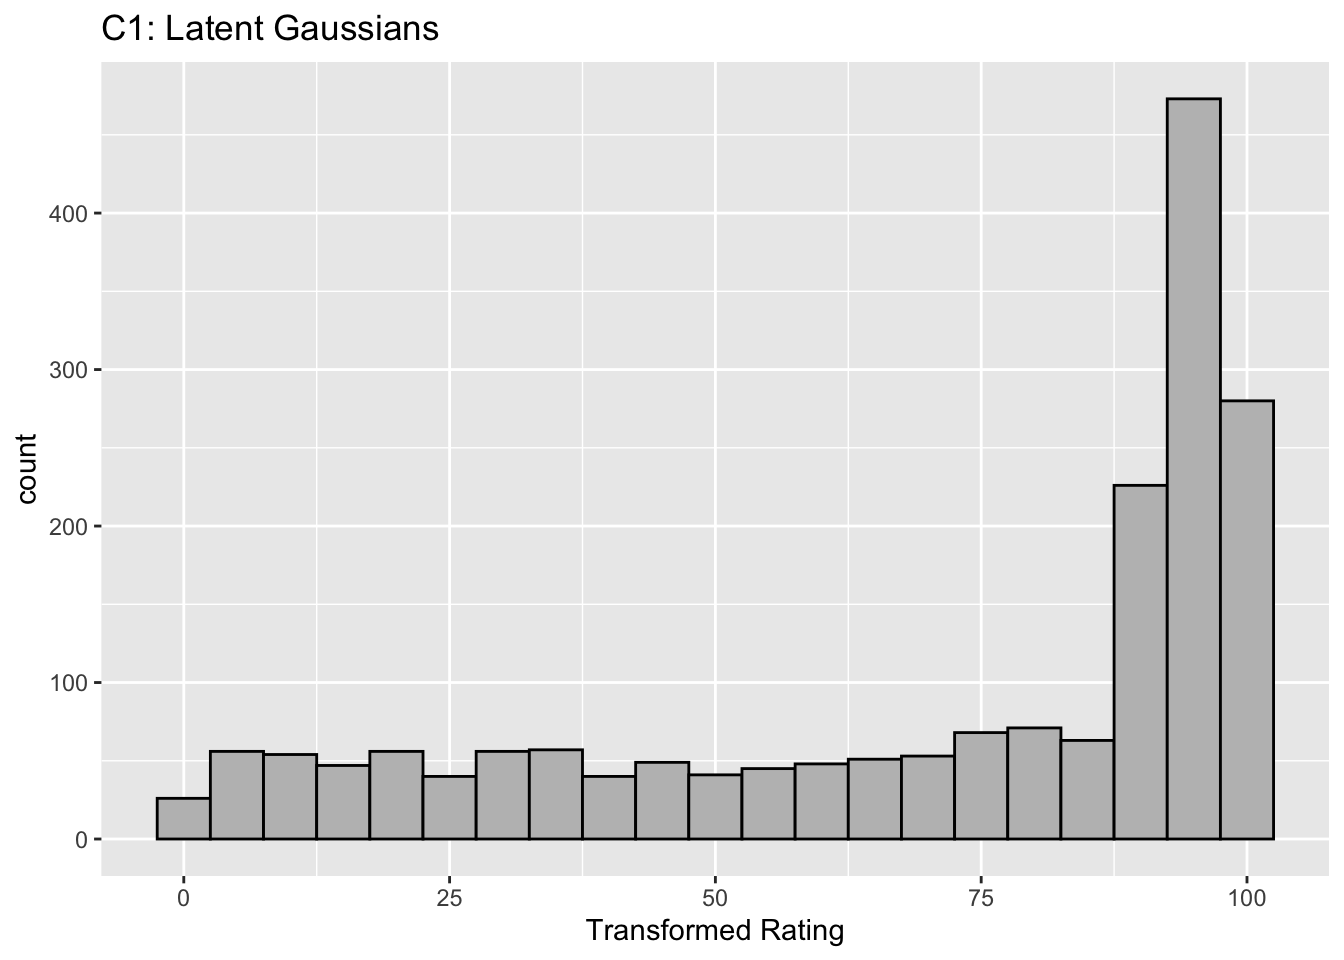
\includegraphics[width=0.33\linewidth]{06-binormal-model_files/figure-latex/unnamed-chunk-6-3} 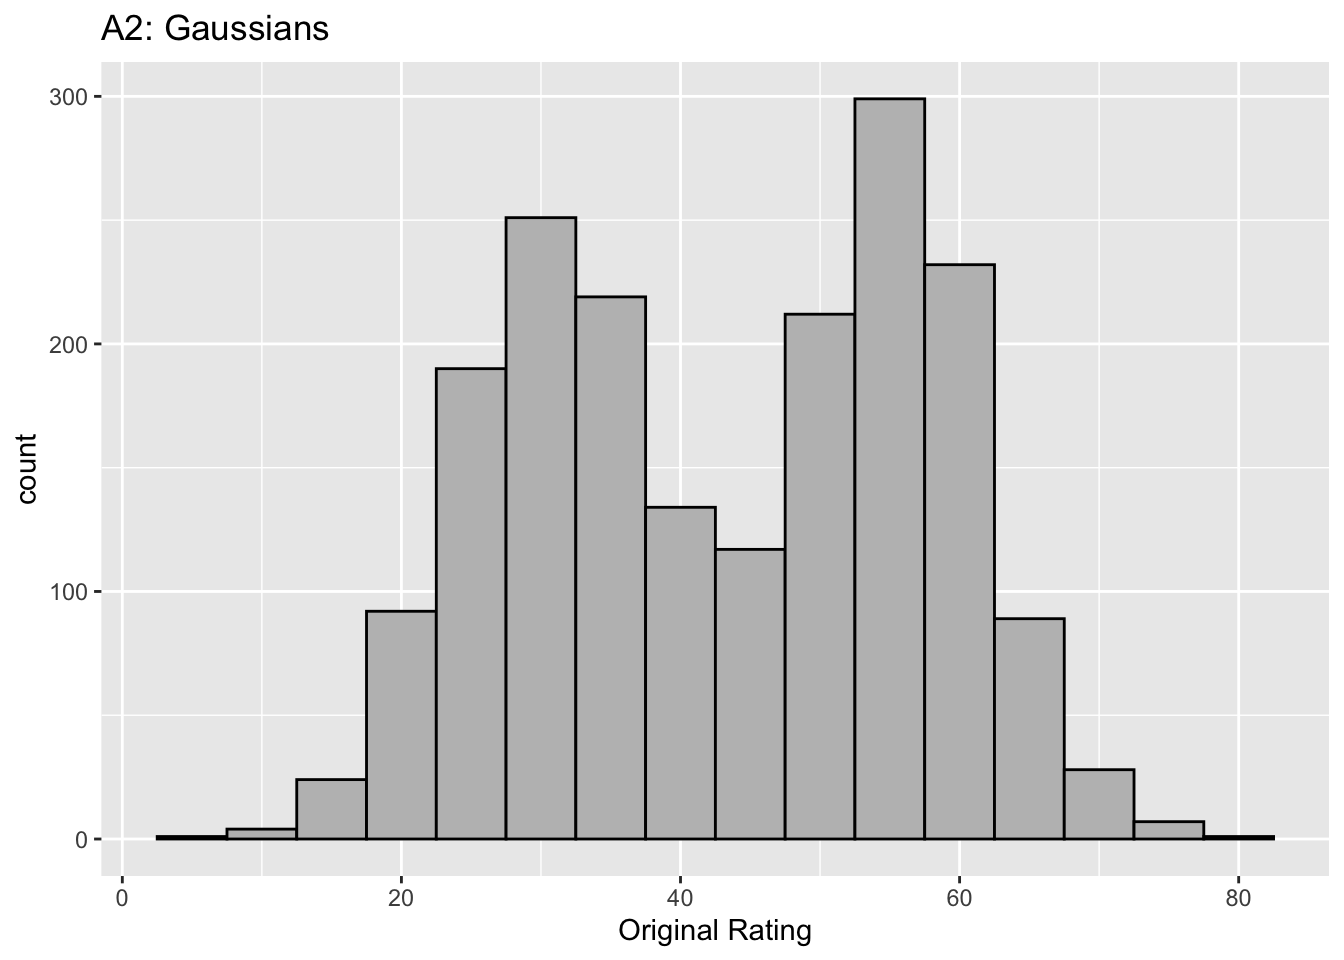
\includegraphics[width=0.33\linewidth]{06-binormal-model_files/figure-latex/unnamed-chunk-6-4} 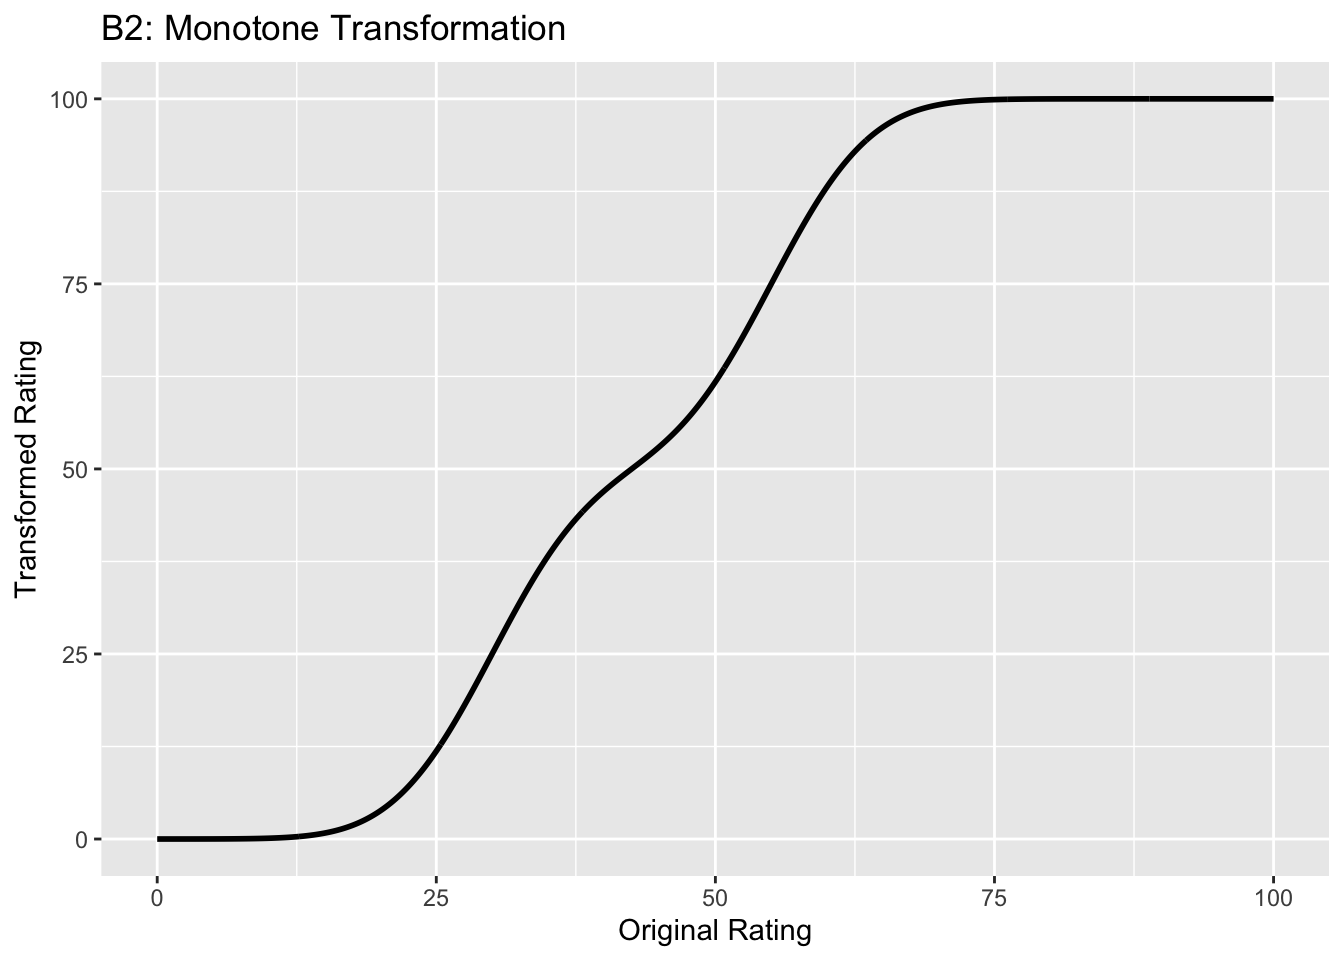
\includegraphics[width=0.33\linewidth]{06-binormal-model_files/figure-latex/unnamed-chunk-6-5} 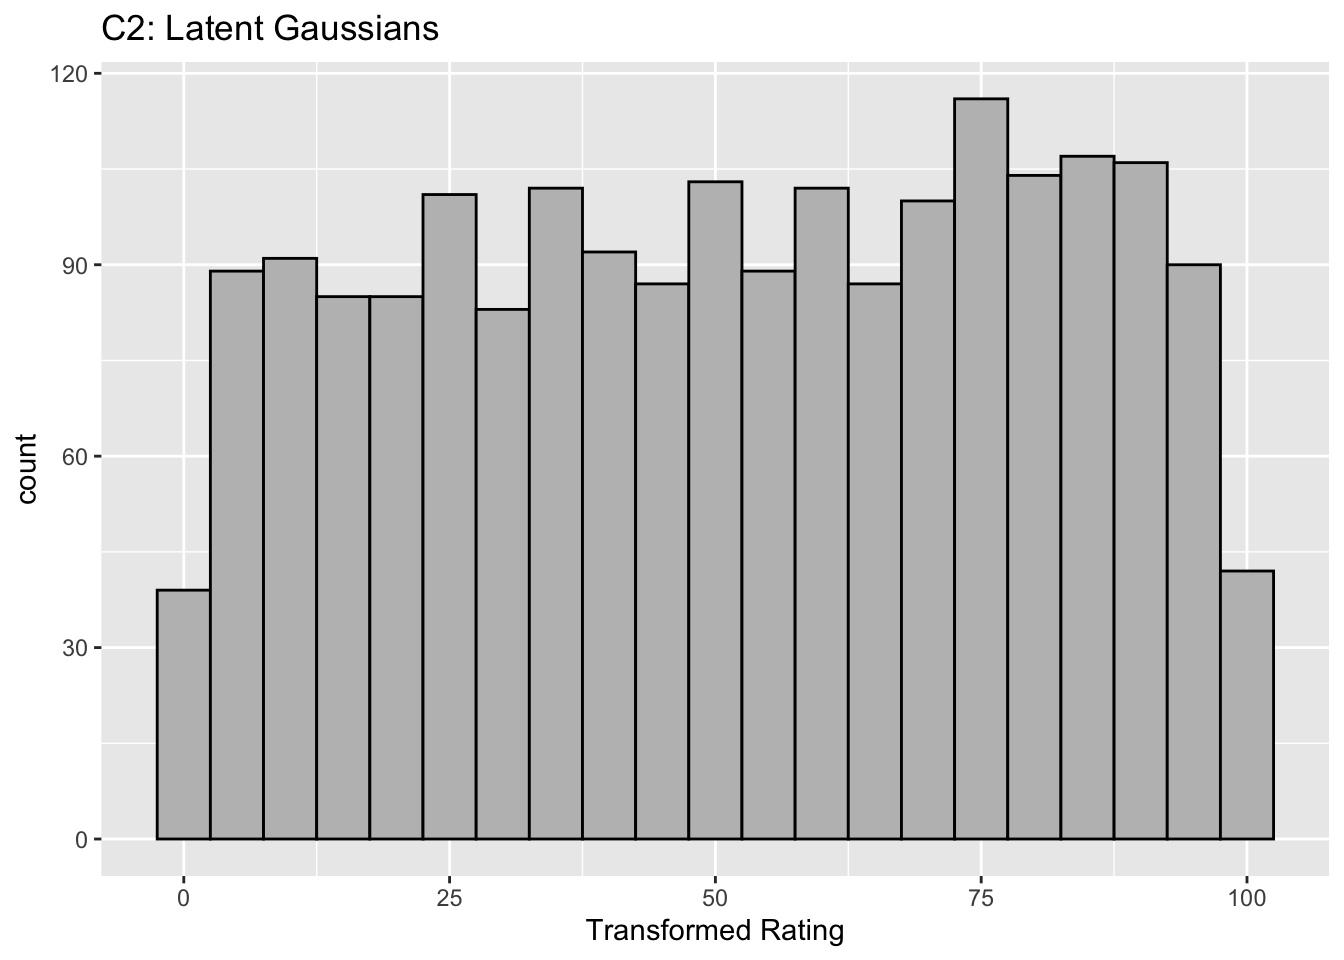
\includegraphics[width=0.33\linewidth]{06-binormal-model_files/figure-latex/unnamed-chunk-6-6} 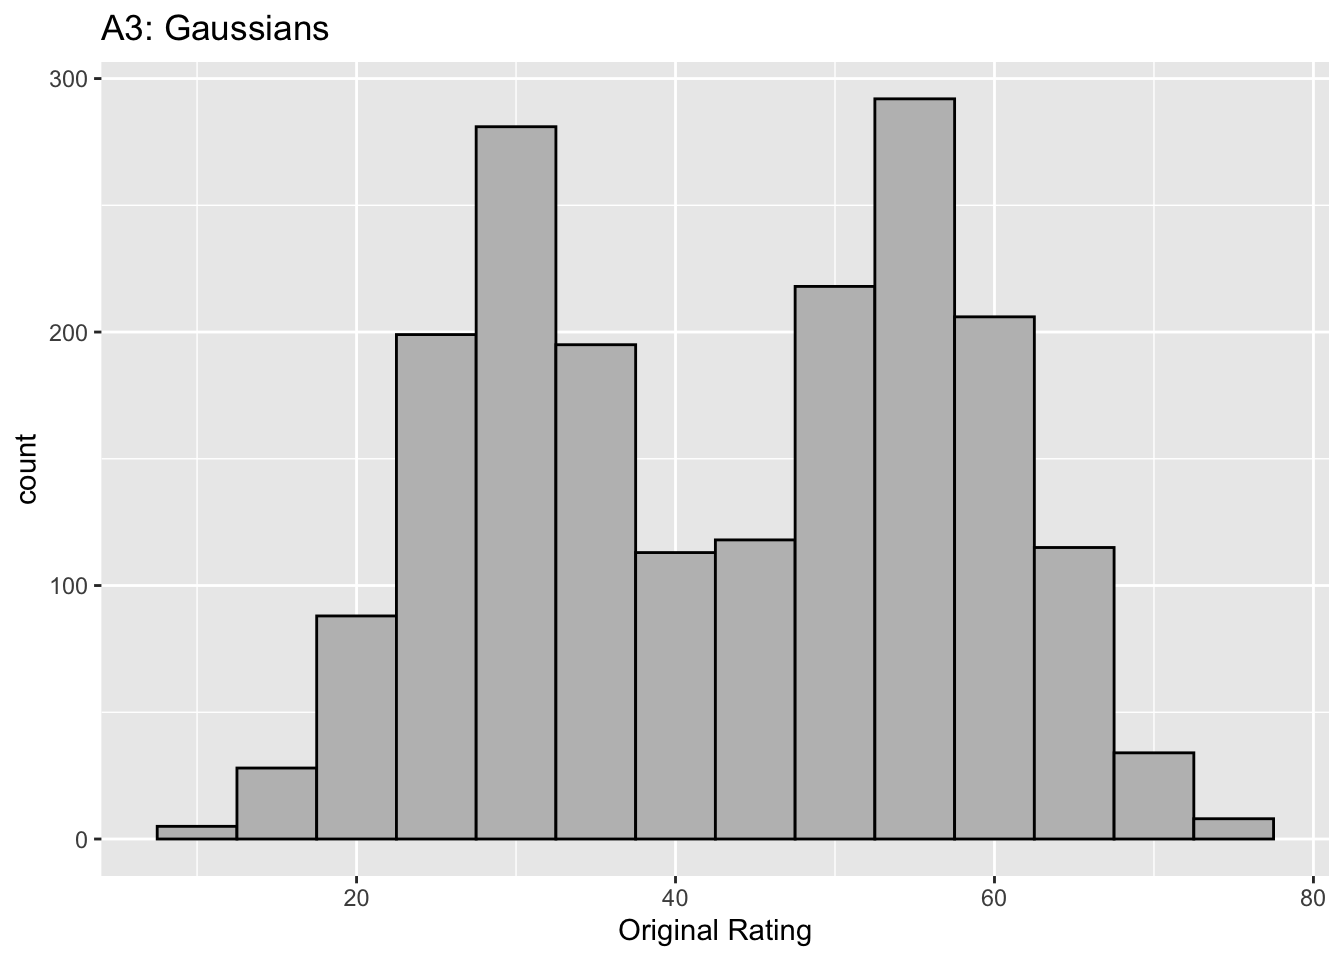
\includegraphics[width=0.33\linewidth]{06-binormal-model_files/figure-latex/unnamed-chunk-6-7} 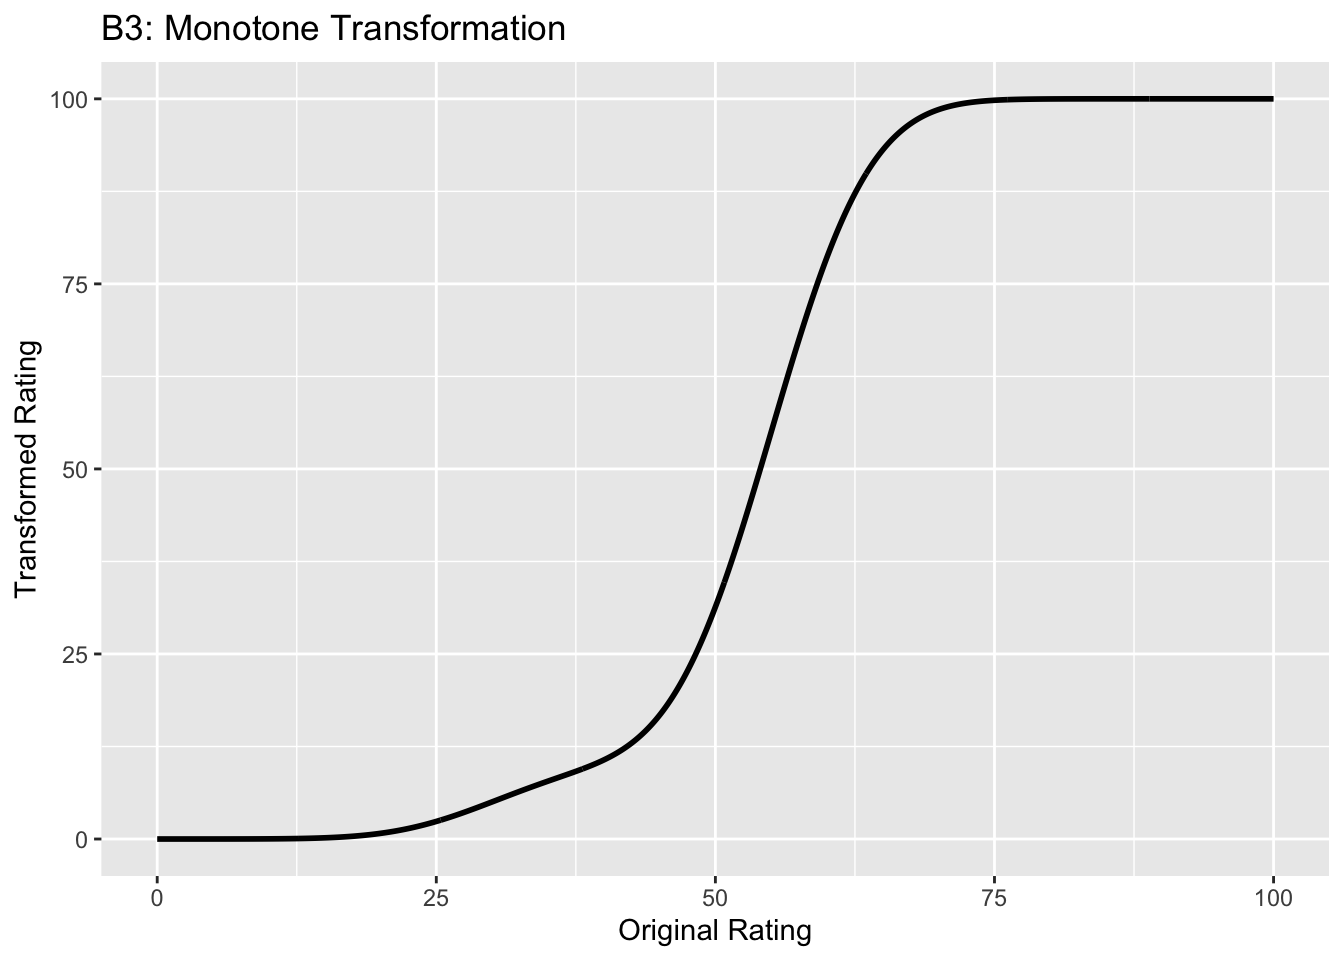
\includegraphics[width=0.33\linewidth]{06-binormal-model_files/figure-latex/unnamed-chunk-6-8} 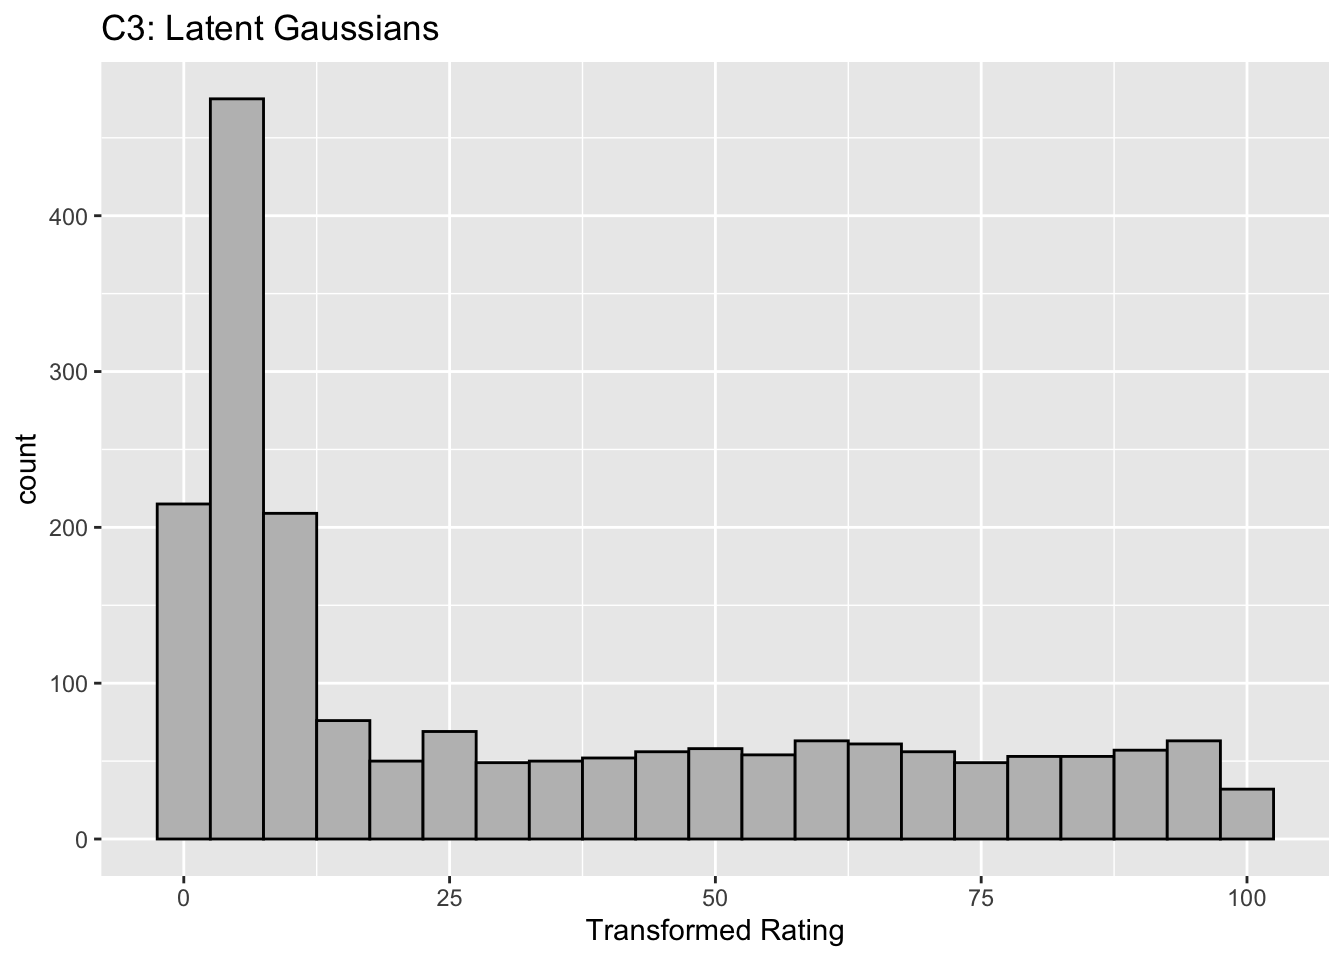
\includegraphics[width=0.33\linewidth]{06-binormal-model_files/figure-latex/unnamed-chunk-6-9}

\textbf{This figure illustrates the invariance of ROC analysis to arbitrary monotone transformations of the ratings.}

\begin{itemize}
\item
  Each row contains 3 plots: labeled 1, 2 and 3. Each column contains 3 plots labeled A, B and C. So, for example, plot C2 refers to the second row and third column. Each of the latent Gaussian plots C1, C2 and C3 appears to be not binormal. However, using the monotone transformations shown (B1, B2 and B3) they can be transformed to the binormal model histograms A1, A2 and A3.
\item
  Plot A1 shows the histogram of simulated ratings from a binormal model. Two peaks, one at 30 and the other at 55 are evident (by design, all ratings in this figure are in the range 0 to 100). Plot B1 shows the monotone transformation. Plot C1 shows the histogram of the transformed rating. The choice of \(f\) leads to a transformed rating histogram that is peaked near the high end of the rating scale. For A1 and C1 the corresponding AUCs are identical.
\item
  Plot A2 is for a different seed value, plot B2 is the transformation and now the transformed histogram is almost flat, plot C2. For plots A2 and C2 the corresponding AUCs are identical.
\item
  Plot A3 is for a different seed value, B3 is the transformation and the transformed histogram C3 is peaked near the low end of the transformed rating scale. For plots A3 and (C3) the corresponding AUCs are identical.
\end{itemize}

\textbf{Visual examination of the shape of the histograms of ratings, or standard tests for normality, yield little, if any, insight into whether the underlying binormal model assumptions are being violated.}

\hypertarget{binormal-model-full-auc}{%
\section{Az and d-prime measures}\label{binormal-model-full-auc}}

The (full) area under the ROC, denoted \(A_z\), is derived in \citep{thompson1989statistical}:

\begin{equation} 
\left.
\begin{aligned}
A_z=&\Phi\left ( \frac{a}{\sqrt{1+b^2}} \right )\\
=&\Phi\left ( \frac{\mu}{\sqrt{1+\sigma^2}} \right )
\end{aligned}
\right\}
\label{eq:binormal-model-ab-2az}
\end{equation}

The binormal fitted AUC increases as \(a\) increases or as \(b\) decreases. Equivalently, it increases as \(\mu\) increases or as \(\sigma\) decreases.

The reason for the name \(A_z\) is that historically (prior to maximum likelihood estimation) this quantity was estimated by converting the probabilities FPF and TPF to \emph{z-deviates} (see TBA), which of-course assumes normal distributions. The z-subscript is meant to emphasize that this is a binormal model derived estimate.

The \(d'\) parameter is defined as the separation of two unit-variance normal distributions yielding the same AUC as that predicted by the \((a,b)\) parameter binormal model. It is defined by:

\begin{equation} 
d'=\sqrt{2}\Phi^{-1}\left ( A_z \right )
\label{eq:binormal-model-ab-2dprime}
\end{equation}

The d' index can be regarded as a perceptual signal-to-noise-ratio.

\hypertarget{binormal-model-fitting}{%
\section{Fitting the binormal model}\label{binormal-model-fitting}}

\citep{dorfman1969maximum} were the first to fit ratings data to the binormal model. The details of the procedure are in Appendix \ref{binormal-model-curve-fitting}. While historically very important in showing how statistically valid quantitative analysis is possible using ROC ratings data, the fitting procedure suffers from what are termed ``degeneracy issues'' and ``fitting artifacts'' discussed in Appendix \ref{binormal-model-degeneracy}. Degeneracy is when the fitting procedure yields unreasonable parameter values. Fitting artifacts occur when the fitted curve predicts worse than chance level performance in some region of the fitted ROC curve. Because of these issues usage of this method is now discouraged as it has largely been supplanted by other software such as the CBM fitting method, the proper ROC fitting method implemented in PROPROC and the RSM (radiological search model) based fitting method. These are discussed in later chapters.

\hypertarget{binormal-model-partial-auc}{%
\section{Partial AUC measures}\label{binormal-model-partial-auc}}

Two partial AUC measures have been defined. The idea is to have an AUC-like measure that emphasizes some region of the ROC curve, one that is argued to be clinically more significant, instead of \(A_z\) which characterizes the whole curve. In the following two definitions are considered, one that emphasizes the high specificity region of the ROC curve and one which emphasizes the high sensitivity region of the curve.

Shorthand: denote \(A \equiv A_z\), \(x \equiv \text{FPF}\) and \(y \equiv \text{TPF}\). The two partial AUC measures correspond to a partial integral along the x-axis starting from the origin (high specificity) and the other to a partial integral along the y-axis ending at (1,1) corresponding to high sensitivity. These are denoted by X and Y superscripts.

\hypertarget{binormal-model-meaning-partial-auc-definitions}{%
\subsection{Measure emphasizing high specificity}\label{binormal-model-meaning-partial-auc-definitions}}

The partial area under the ROC, \(A_c^{X}\), is defined as that extending from \(x = 0\) to \(x = c\), where \(0 \le c \le 1\) (in our notation \(c\) always means a cutoff on the x-axis of the ROC):

\begin{equation} 
\left. 
\begin{aligned}
A_c^{X} &= \int_{x=0}^{x=c} y \, dx 
\\&=  \int_{x=0}^{x=c} \Phi\left ( a + b \; \Phi^{-1} \left ( x \right ) \right ) \, dx 
\end{aligned}
\right \}
\label{eq:binormal-model-partial-area-a1}
\end{equation}

The second form follows from Eqn. \eqref{eq:binormal-model-roc-curve-tpf-fpf}.

\citep{thompson1989statistical} derive a formula for the partial-area in terms of the binormal model parameters \(a\) and \(b\):

\begin{equation}
A_c^{X} = \int_{z_2=-\infty}^{\Phi^{-1}\left ( c \right )}   \int_{z_1=-\infty}^{\frac{a}{\sqrt{1+b^2}}} \phi\left ( z_1,z_2;\rho \right ) dz_1dz_2
\label{eq:binormal-model-partial-area-final}
\end{equation}

On the right hand side the integrand \(\phi\left ( z_1,z_2;\rho \right )\) is the standard bivariate normal density function with correlation coefficient \(\rho\). It is defined by:

\begin{equation}
\left. 
\begin{aligned}
\phi\left (z_1,z_2;\rho \right ) &= \frac{1}{2 \pi \sqrt{1-\rho^2}} \exp\left ( -\frac{z_1^2 -2\rho z_1 z_2 +z_2^2}{2\left ( 1-\rho^2 \right )} \right ) \\
\rho &= - \frac{b}{\sqrt{1+b^2}}
\end{aligned}
\right \}
\label{eq:binormal-model-bivariate-density}
\end{equation}

As demonstrated later the integrals occurring on the right hand side of Eqn. \eqref{eq:binormal-model-partial-area-final} can be evaluated numerically.

As an area measure the partial AUC \(A_c^{X}\) has a simple \emph{geometric} meaning. A \emph{physical} meaning is as follows:

\begin{quote}
An ROC curve\footnote{This curve is not binormal as the truncation destroys the normality of the two distributions} can be defined over the truncated dataset where all z-samples \textbf{smaller} than \(-\Phi^{-1}(c)\) are ignored. The maximum area of this curve is that defined by the rectangle with corners at \((0,0)\) and \((c,\text{TPF}\left ( c \right ))\): \(c\) is the abscissa at the upper limit of the integration interval along the x-axis and \(\text{TPF}\left ( c \right )\) is the corresponding ordinate: see Eqn. \eqref{eq:binormal-model-roc-curve-tpf-fpf}. Dividing \(A_c^{X}\) by \(\text{TPF}\left ( c \right ) \times c\) yields a normalized partial area measure, denoted \(A_c^{XN}\), where \(0 \le A_c^{XN} \le 1\). \textbf{This is the classification accuracy between diseased and non-diseased cases measured over the truncated dataset.} If \(a \ge 0\) it is constrained to (0.5, 1).
\end{quote}

\begin{equation}
A_c^{XN} = \frac{A_c^{X}}{\text{TPF}\left ( c \right ) \times c}
\label{eq:binormal-model-normalized-partial-auc-specificity}
\end{equation}

\hypertarget{binormal-model-metz-partial-auc}{%
\subsection{Measure emphasizing high sensitivity}\label{binormal-model-metz-partial-auc}}

Since the integral in Eqn. \eqref{eq:binormal-model-partial-area-a1} is from \(x = 0\) to \(x = c\) this partial AUC measure emphasizes the \emph{high specificity} region of the ROC curve (since \(x = 0\) corresponds to unit, i.e.~highest, specificity).

An alternative partial AUC measure has been defined \citep{jiang1996receiver} that emphasizes the \emph{high sensitivity} region of the ROC as follows:

\begin{equation} 
A_c^{Y} = \int_{y=\text{TPF}(c)}^{y=1} \left (1-x  \right ) \, dy
\label{eq:binormal-model-partial-area-ac-metz}
\end{equation}

\(A_c^{Y}\) is the (un-normalized) area below the ROC extending from \(y = \text{TPF}(c)\) to \(y = 1\). The superscript Y denotes that the integral is over part of the y-axis. The maximum value of this integral is the area of the rectangle defined by the corner points \((c,\text{TPF}(c))\) and \((1,1)\). Therefore the normalized area is defined by (our normalization differs from that in the cited reference):

\begin{equation}
A_c^{YN} = \frac{A_c^{Y}}{\left (1 - \text{TPF}(c)  \right ) \times \left (1-c  \right )}
\label{eq:binormal-model-normalized-partial-auc-sensitivity}
\end{equation}

A \emph{physical} meaning is as follows:

\begin{quote}
An ROC curve can be defined over the truncated dataset where all z-samples \textbf{greater} than \(-\Phi^{-1}(c)\) are ignored. \textbf{\(A_c^{YN}\) is the classification accuracy between diseased and non-diseased cases measured over the truncated dataset.} By definition the normalized area ranges between 0 and 1.
\end{quote}

\hypertarget{binormal-model-metz-partial-auc-example}{%
\subsection{Numerical examples}\label{binormal-model-metz-partial-auc-example}}

Fig. \ref{fig:binormal-model-partial-areas} shows the two un-normalized areas.

\begin{figure}
\centering
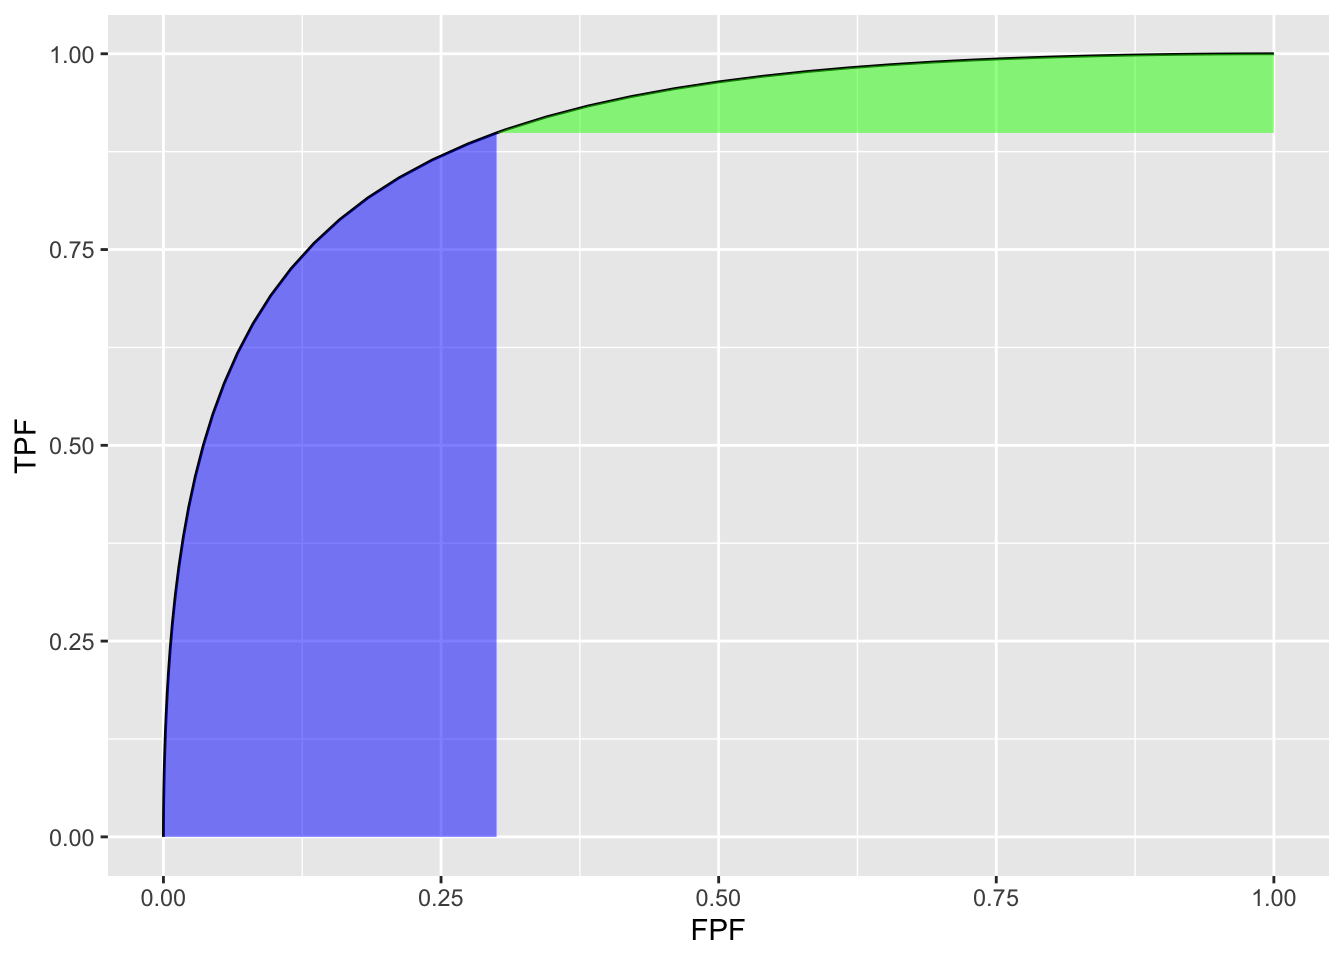
\includegraphics{06-binormal-model_files/figure-latex/binormal-model-partial-areas-1.pdf}
\caption{\label{fig:binormal-model-partial-areas}Un-normalized partial AUC measures: the blue shaded area is \(A_c^{X}\), the partial area below the ROC; the green shaded area is \(A_c^{Y}\) the partial area above the ROC. Parameters are \(a = 1.8\), \(b = 1\) and \(c = 0.3\).}
\end{figure}

The following code illustrates calculation of the partial-area measure using the function \texttt{pmvnorm} in the \texttt{R} package \texttt{mvtnorm} \citep{R-mvtnorm}. The parameter values were: \(a = 1.8\), \(b = 1\) and \(c = 0.3\) (see lines 1-3 below).

\begin{Shaded}
\begin{Highlighting}[numbers=left,,]
\NormalTok{a }\OtherTok{\textless{}{-}} \FloatTok{1.8}
\NormalTok{b }\OtherTok{\textless{}{-}} \DecValTok{1}
\NormalTok{fpf\_c }\OtherTok{\textless{}{-}} \FloatTok{0.3} \CommentTok{\# cannot use c as variable name}
\NormalTok{tpf\_c }\OtherTok{\textless{}{-}} \FunctionTok{pnorm}\NormalTok{(a }\SpecialCharTok{+}\NormalTok{ b }\SpecialCharTok{*} \FunctionTok{qnorm}\NormalTok{(fpf\_c))}
\NormalTok{A\_z }\OtherTok{\textless{}{-}} \FunctionTok{pnorm}\NormalTok{(a}\SpecialCharTok{/}\FunctionTok{sqrt}\NormalTok{(}\DecValTok{1}\SpecialCharTok{+}\NormalTok{b}\SpecialCharTok{\^{}}\DecValTok{2}\NormalTok{))}
\NormalTok{rho }\OtherTok{\textless{}{-}} \SpecialCharTok{{-}}\NormalTok{b}\SpecialCharTok{/}\FunctionTok{sqrt}\NormalTok{(}\DecValTok{1}\SpecialCharTok{+}\NormalTok{b}\SpecialCharTok{\^{}}\DecValTok{2}\NormalTok{)}
\NormalTok{Lower1 }\OtherTok{\textless{}{-}} \SpecialCharTok{{-}}\ConstantTok{Inf}
\NormalTok{Upper1 }\OtherTok{\textless{}{-}} \FunctionTok{qnorm}\NormalTok{(fpf\_c)}
\NormalTok{Lower2 }\OtherTok{\textless{}{-}} \SpecialCharTok{{-}}\ConstantTok{Inf}
\NormalTok{Upper2 }\OtherTok{\textless{}{-}}\NormalTok{ a}\SpecialCharTok{/}\FunctionTok{sqrt}\NormalTok{(}\DecValTok{1}\SpecialCharTok{+}\NormalTok{b}\SpecialCharTok{\^{}}\DecValTok{2}\NormalTok{)}
\NormalTok{sigma }\OtherTok{\textless{}{-}} \FunctionTok{rbind}\NormalTok{(}\FunctionTok{c}\NormalTok{(}\DecValTok{1}\NormalTok{, rho), }\FunctionTok{c}\NormalTok{(rho, }\DecValTok{1}\NormalTok{))}
\NormalTok{A\_x }\OtherTok{\textless{}{-}} \FunctionTok{as.numeric}\NormalTok{(}\FunctionTok{pmvnorm}\NormalTok{(}
  \FunctionTok{c}\NormalTok{(Lower1, Lower2), }
  \FunctionTok{c}\NormalTok{(Upper1, Upper2), }
  \AttributeTok{sigma =}\NormalTok{ sigma))}

\CommentTok{\# divide by area of rectangle}
\NormalTok{A\_xn }\OtherTok{\textless{}{-}}\NormalTok{ A\_x}\SpecialCharTok{/}\NormalTok{fpf\_c}\SpecialCharTok{/}\NormalTok{tpf\_c}
\end{Highlighting}
\end{Shaded}

The function \texttt{pmvnorm} is called at line 12. The un-normalized partial-area measure \(A_c^{X}\) = 0.216. The corresponding full AUC measure is \(A_z\) = 0.898. The normalized measure is \(A_c^{XN}\) = 0.802. This is the classification accuracy between non-diseased and diseased cases in the truncated dataset defined by ignoring cases with z-samples smaller than \(-\Phi^{-1}(c)\) = 0.524. This measure emphasizes specificity.

\(A_c^{Y}\) can be calculated using geometry. One subtracts \(A_c^{X}\) from \(A_z\) to get the area under the ROC to the right of \(\text{FPF}=c\). Next one subtracts from this quantity the area of the rectangle with base \((1 - c)\) and height \(\text{TPF}_c\). This yields the area if the green shaded region \(A_c^{Y}\). To normalize it one divides by the area of the rectangle defined by the corner points \((c,\text{TPF}_c)\) and (1,1).

\begin{Shaded}
\begin{Highlighting}[]
\CommentTok{\# implement geometrical logic}
\NormalTok{A\_y }\OtherTok{\textless{}{-}}\NormalTok{ (A\_z }\SpecialCharTok{{-}}\NormalTok{ A\_x)}\SpecialCharTok{{-}}\NormalTok{(}\DecValTok{1}\SpecialCharTok{{-}}\NormalTok{fpf\_c)}\SpecialCharTok{*}\NormalTok{(tpf\_c)}
\NormalTok{A\_yn }\OtherTok{\textless{}{-}}\NormalTok{ A\_y}\SpecialCharTok{/}\NormalTok{(}\DecValTok{1}\SpecialCharTok{{-}}\NormalTok{tpf\_c)}\SpecialCharTok{/}\NormalTok{(}\DecValTok{1}\SpecialCharTok{{-}}\NormalTok{fpf\_c) }
\end{Highlighting}
\end{Shaded}

The un-normalized partial-area measure \(A_c^{Y}\) = 0.053. The normalized measure is \(A_c^{YN}\) = 0.748. This is the classification accuracy between non-diseased and diseased cases in the truncated dataset defined by ignoring cases with z-samples greater than \(-\Phi^{-1}(c)\) = 0.524. This measure emphasizes sensitivity.

The variation with \(a\) of the two normalized AUC measures is shown next. The function \texttt{normalizedAreas} encapsulates the above calculations and is called for different values of \(a\).

\begin{Shaded}
\begin{Highlighting}[]
\NormalTok{a\_arr }\OtherTok{=} \FunctionTok{seq}\NormalTok{(}\DecValTok{0}\NormalTok{,}\DecValTok{8}\NormalTok{)}
\NormalTok{A\_xn\_arr }\OtherTok{\textless{}{-}} \FunctionTok{array}\NormalTok{(}\AttributeTok{dim =} \FunctionTok{length}\NormalTok{(a\_arr))}
\NormalTok{A\_yn\_arr }\OtherTok{\textless{}{-}} \FunctionTok{array}\NormalTok{(}\AttributeTok{dim =} \FunctionTok{length}\NormalTok{(a\_arr))}
\ControlFlowTok{for}\NormalTok{ (i }\ControlFlowTok{in} \DecValTok{1}\SpecialCharTok{:}\FunctionTok{length}\NormalTok{(a\_arr)) \{}
\NormalTok{  x }\OtherTok{\textless{}{-}} \FunctionTok{normalizedAreas}\NormalTok{(a\_arr[i], }\DecValTok{1}\NormalTok{, }\FloatTok{0.1}\NormalTok{) }\CommentTok{\# c = 0.1}
\NormalTok{  A\_xn\_arr[i] }\OtherTok{\textless{}{-}}\NormalTok{ x}\SpecialCharTok{$}\NormalTok{A\_xn}
\NormalTok{  A\_yn\_arr[i] }\OtherTok{\textless{}{-}}\NormalTok{ x}\SpecialCharTok{$}\NormalTok{A\_yn}
\NormalTok{\}}
\end{Highlighting}
\end{Shaded}

\begin{table}

\caption{\label{tab:summary-table-partial-normalized-areas}Summary of normalized $A_c^{XN}$ and $A_c^{YN}$ partial AUCs for different values of the $a$ parameter, where $b = 1$ and $c = 0.1$.}
\centering
\begin{tabular}[t]{r|r|r}
\hline
$a$ & $A^{XN}_c$ & $A^{YN}_c$\\
\hline
0 & 0.5000 & 0.5000\\
\hline
1 & 0.6260 & 0.7015\\
\hline
2 & 0.7785 & 0.8208\\
\hline
3 & 0.9144 & 0.8842\\
\hline
4 & 0.9822 & 0.9189\\
\hline
5 & 0.9981 & 0.9393\\
\hline
6 & 0.9999 & 0.9521\\
\hline
7 & 1.0000 & 0.9608\\
\hline
8 & 1.0000 & 0.9670\\
\hline
\end{tabular}
\end{table}

Table \ref{tab:summary-table-partial-normalized-areas} shows \(A_c^{XN}\) and \(A_c^{YN}\) partial AUCs for different values of the \(a\) parameter for \(b = 1\) and \(c = 0.1\). It demonstrates that the normalized areas are constrained between 0.5 and 1 (as long as \(a\) in non-negative). For numerical reasons (basically a zero-divided-by-zero condition) it is difficult to show that \(A_c^{YN}\) approaches 1 in the limit of very large a-parameter (since the green shaded area shrinks to zero).

\hypertarget{binormal-model-partial-auc-comments}{%
\section{Comments on partial AUC measures}\label{binormal-model-partial-auc-comments}}

There are several issues with the adoption of either partial AUC measure.

\begin{enumerate}
\def\labelenumi{\arabic{enumi}.}
\item
  Since a partial area measure corresponds to classification accuracy measured over a \textbf{truncated} dataset a fundamental correspondence between \(A_z\) and classification accuracy measured over the \textbf{entire} dataset is lost. A basic statistical principle of the desirability of an estimate valid for the entire population is being violated.
\item
  The choice of the truncation cutoff is arbitrary and subject to bias on the part of the investigator. This is similar to the type of bias that is inherent in a single point (sensitivity-specificity) based approach to analysis: this was the very reason for adoption of a measure such as \(A_z\) that averages over the whole curve, as argued so eloquently in \citep{metz1978rocmethodology}.
\item
  Then there is the issue of possible loss of statistical power. If \(A_z\) is estimated from the whole dataset and either Eqn. \eqref{eq:binormal-model-normalized-partial-auc-specificity} or Eqn. \eqref{eq:binormal-model-normalized-partial-auc-sensitivity} is used to estimate partial AUC, then one expects no loss in statistical power, as these equations represent noiseless mathematical transformations using the \((a,b)\) parameters estimated over the entire dataset. However, if an empirical partial AUC measure is used there will surely be loss of statistical power resulting from ignoring some of the data. Due to degeneracy issues usage of the empirical partial AUC is often unavoidable. This is because performing significance testing requires that the dataset be re-sampled many times and the parametric fit may not work every time.
\end{enumerate}

The second point is illustrated by the study reported in \citep{jiang1996receiver}. The ROC curves of a developmental-stage CAD system and that of radiologists cross each other: at high specificity the radiologists were better but the reverse was true at high sensitivity. By choosing the latter region the authors demonstrated statistically significant superiority of CAD over radiologists. Analysis using \(A_z\) failed to reach statistical significance.

Two very large clinical studies \citep[\citet{fenton2011effectiveness}]{fenton2007influence} using 222,135 and 684,956 women, respectively, showed that a commercial CAD can actually have a detrimental effect on patient outcome\citep{philpotts2009can}. A more recent study has confirmed the negative view of the efficacy of CAD\citep{lehman2015diagnostic} and there has even been a call for ending Medicare reimbursement for CAD interpretations\citep{fenton2015time}. I have not followed the field since ca. 2016 and it is likely that newer versions of CAD now being used in the clinic are better than those evaluated in the cited studies. But the point is that even using a ca. 1996 developmental-stage CAD the authors were able to claim, using a partial AUC measure, that CAD outperformed radiologists, a result clearly not borne out by later large clinical studies while the \(A_z\) measure did not allow this conclusion.

\hypertarget{binormal-model-discussion}{%
\section{Discussion}\label{binormal-model-discussion}}

The binormal model is historically very important and the contribution by Dorfman and Alf \citep{dorfman1969maximum} was seminal. Prior to their work, there was no statistically valid way of estimating AUC from observed ratings counts. Their work and a key paper \citep{RN1487} accelerated research using ROC methods. The number of publications using their algorithm, and the more modern versions developed by Metz and colleagues, is probably well in excess of 500. Because of its key role, I have endeavored to take out some of the mystery about how the binormal model parameters are estimated. In particular, a common misunderstanding that the binormal model assumptions are violated by real datasets, when in fact it is quite robust to apparent deviations from normality, is addressed (details are in Section \ref{binormal-model-invariance-property}).

A good understanding of this chapter should enable the reader to better understand alternative ROC models, discussed later.

To this day the binormal model is widely used to fit ROC datasets. In spite of its limitations, the binormal model has been very useful in bringing a level of quantification to this field that did not exist prior to 1969.

\hypertarget{binormal-model-curve-fitting}{%
\section{Appendix: Fitting an ROC curve}\label{binormal-model-curve-fitting}}

One aim of this chapter is to demystify statistical curve fitting. With the passing of Profs. Donald Dorfman, Charles Metz and Richard Swensson, parametric modeling is much neglected. Researchers have instead focused on non-parametric analysis using the empirical AUC defined in Chapter \ref{empirical-auc}. A claimed advantage (overstated in my opinion, see Section \ref{binormal-model-invariance-property}) of non-parametric analysis is the absence of distributional assumptions. Non-parametric analysis yields no insight into what is limiting performance. Binormal model based curve fitting described in this chapter will allow the reader to appreciate a later chapter (see RSM fitting chapter in \texttt{RJafrocFrocBook}) that describes a more complex fitting method which yields important insights into the factors limiting human observer (or artificial intelligence algorithm) performance.

\hypertarget{java-fitted-roc-curve}{%
\subsection{JAVA fitted ROC curve}\label{java-fitted-roc-curve}}

This section, described in the physical book, has been abbreviated to a \href{http://www.rad.jhmi.edu/jeng/javarad/roc/JROCFITi.html}{relevant website}.

\hypertarget{simplistic-straight-line-fit-to-the-roc-curve}{%
\subsection{Simplistic straight line fit to the ROC curve}\label{simplistic-straight-line-fit-to-the-roc-curve}}

To be described next is a method for fitting data such as in Table \ref{tab:ratings-paradigm-example-table} to the binormal model, i.e., determining the parameters \((a,b)\) and the thresholds \(\zeta_r , \quad r = 1, 2, ..., R-1\), to best fit, in some to-be-defined sense, the observed cell counts. The most common method uses an algorithm called maximum likelihood. But before getting to that, I describe the least-square method, which is conceptually simpler, but not really applicable, as will be explained shortly.

\hypertarget{least-squares-estimation}{%
\subsubsection{Least-squares estimation}\label{least-squares-estimation}}

By applying the function \(\Phi^{-1}\) to both sides of Eqn. \eqref{eq:binormal-model-roc-curve1}, one gets (the ``inverse'' function cancels the ``forward'' function on the right hand side):

\begin{equation*} 
\Phi^{-1}\left ( \text{TPF} \right ) = a + b \Phi^{-1}\left ( FPF \right )
\end{equation*}

This suggests that a plot of \(y = \Phi^{-1}\left ( \text{TPF} \right )\) vs.~\(x=\Phi^{-1}\left ( FPF \right )\) is expected to follow a straight line with slope \(b\) and intercept \(a\). Fitting a straight line to such data is generally performed by the method of least-squares, a capability present in most software packages and spreadsheets. Alternatively, one can simply visually draw the best straight line that fits the points, memorably referred to \citep{RN300} as ``chi-by-eye''. This was the way parameters of the binormal model were estimated prior to Dorfman and Alf's work \citep{dorfman1969maximum}. The least-squares method is a quantitative way of accomplishing the same aim. If \(\left ( x_t,y_t \right )\) are the data points, one constructs \(S\), the sum of the squared deviations of the observed ordinates from the predicted values (since \(R\) is the number of ratings bins, the summation runs over the \(R-1\) operating points):

\begin{equation*} 
S  = \sum_{i=1}^{R-1}\left ( y_i - \left ( a + bx_i \right ) \right )^2
\end{equation*}

The idea is to minimize S with respect to the parameters \((a,b)\). One approach is to differentiate this with respect to \(a\) and \(b\) and equate each resulting derivate expression to zero. This yields two equations in two unknowns, which are solved for \(a\) and \(b\). If the reader has never done this before, one should go through these steps at least once, but it would be smarter in future to use software that does all this. In \texttt{R} the least-squares fitting function is \texttt{lm(y\textasciitilde{}x)}, which in its simplest form fits a linear model \texttt{lm(y\textasciitilde{}x)} using the method of least-squares (in case you are wondering \texttt{lm} stands for linear model, a whole branch of statistics in itself; in this example one is using its simplest capability).

\begin{Shaded}
\begin{Highlighting}[]
\CommentTok{\# ML estimates of a and b (from Eng JAVA program)}
\CommentTok{\# a \textless{}{-} 1.3204; b \textless{}{-} 0.6075 }
\CommentTok{\# \# these are not used in program; just here for comparison}

\NormalTok{FPF }\OtherTok{\textless{}{-}} \FunctionTok{c}\NormalTok{(}\FloatTok{0.017}\NormalTok{, }\FloatTok{0.050}\NormalTok{, }\FloatTok{0.183}\NormalTok{, }\FloatTok{0.5}\NormalTok{)  }
\CommentTok{\# this is from Table 6.11, last two rows}
\NormalTok{TPF }\OtherTok{\textless{}{-}} \FunctionTok{c}\NormalTok{(}\FloatTok{0.440}\NormalTok{, }\FloatTok{0.680}\NormalTok{, }\FloatTok{0.780}\NormalTok{, }\FloatTok{0.900}\NormalTok{)}
\CommentTok{\# ...do...}

\NormalTok{PhiInvFPF }\OtherTok{\textless{}{-}} \FunctionTok{qnorm}\NormalTok{(FPF)}
\CommentTok{\# apply the PHI\_INV function}
\NormalTok{PhiInvTPF }\OtherTok{\textless{}{-}} \FunctionTok{qnorm}\NormalTok{(TPF)}
\CommentTok{\# ... do ... }

\NormalTok{fit }\OtherTok{\textless{}{-}} \FunctionTok{lm}\NormalTok{(PhiInvTPF}\SpecialCharTok{\textasciitilde{}}\NormalTok{PhiInvFPF)}
\FunctionTok{print}\NormalTok{(fit)}
\CommentTok{\#\textgreater{} }
\CommentTok{\#\textgreater{} Call:}
\CommentTok{\#\textgreater{} lm(formula = PhiInvTPF \textasciitilde{} PhiInvFPF)}
\CommentTok{\#\textgreater{} }
\CommentTok{\#\textgreater{} Coefficients:}
\CommentTok{\#\textgreater{} (Intercept)    PhiInvFPF  }
\CommentTok{\#\textgreater{}    1.328844     0.630746}
\end{Highlighting}
\end{Shaded}

\begin{figure}
\centering
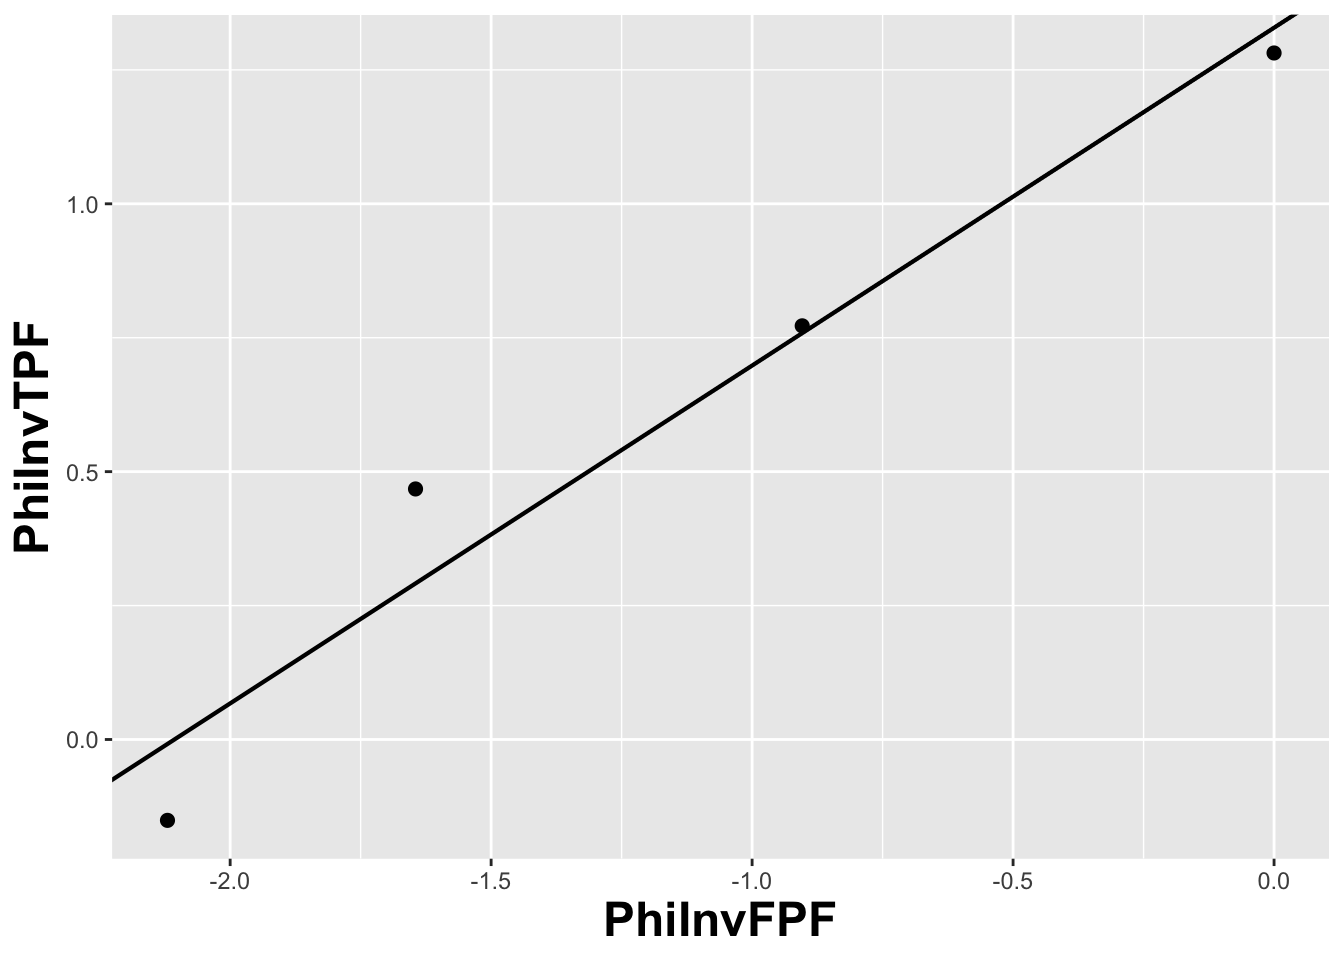
\includegraphics{06-binormal-model_files/figure-latex/binormal-model-line-fit-1.pdf}
\caption{\label{fig:binormal-model-line-fit}The straight line fit method of estimating parameters of the fitting model.}
\end{figure}

Fig. \ref{fig:binormal-model-line-fit} shows operating points from Table \ref{tab:ratings-paradigm-example-table}, transformed by the \(\Phi^{-1}\) function; the slope of the line is the least-squares estimate of the \(b\) parameter and the intercept is the corresponding \(a\) parameter of the binormal model.

The last line contains the least squares estimated values, \(a\) = 1.3288 and \(b\) = 0.6307. The corresponding maximum likelihood estimates of these parameters, as yielded by the Eng web code, see Appendix, are listed in line 4 of the main program: \(a\) = 1.3204 and \(b\) = 0.6075. The estimates appear to be close, particularly the estimate of \(a\) , but there are a few things wrong with the least-squares approach. First, the method of least squares assumes that the data points are independent. Because of the manner in which they are constructed, namely by cumulating points, the independence assumption is not valid for ROC operating points. Cumulating the 4 and 5 responses constrains the resulting operating point to be above and to the right of the point obtained by cumulating the 5 responses only, so the data points are definitely not independent. Similarly, cumulating the 3, 4 and 5 responses constrains the resulting operating point to be above and to the right of the point obtained by cumulating the 4 and 5 responses, and so on. The second problem is the linear least-squares method assumes there is no error in measuring x; the only source of error that is accounted for is in the y-coordinate. In fact, both coordinates of an ROC operating point are subject to sampling error. Third, disregard of error in the x-direction is further implicit in the estimates of the thresholds, which according to Eqn. (6.2.19), is given by:

\begin{equation*} 
\zeta_r = - \Phi^{-1}\left ( FPF_r \right )
\end{equation*}

These are ``rigid'' estimates that assume no error in the FPF values. As was shown in Chapter \ref{binary-task}, 95\% confidence intervals apply to these estimates.

A historical note: prior to computers and easy access to statistical functions the analyst had to use a special plotting paper, termed ``double probability paper'', that converted probabilities into x and y distances using the inverse function.

\hypertarget{maximum-likelihood-estimation-mle}{%
\subsection{Maximum likelihood estimation (MLE)}\label{maximum-likelihood-estimation-mle}}

The approach taken by Dorfman and Alf was to maximize the likelihood function instead of S. The likelihood function is the probability of the observed data given a set of parameter values, i.e.,

\begin{equation*} 
\text {L} \equiv P\left ( data \mid \text {parameters} \right )
\end{equation*}

Generally ``data'' is suppressed, so likelihood is a function of the parameters; but ``data'' is always implicit. With reference to Fig. 6.1, the probability of a non-diseased case yielding a count in the 2nd bin equals the area under the curve labeled ``Noise'' bounded by the vertical lines at \(\zeta_1\) and \(\zeta_2\). In general, the probability of a non-diseased case yielding a count in the \(r^\text{th}\) bin equals the area under the curve labeled ``Noise'' bounded by the vertical lines at \(\zeta_{r-1}\) and \(\zeta_r\). Since the area to the left of a threshold is the CDF corresponding to that threshold, the required probability is \(\Phi\left ( \zeta_r \right ) - \Phi\left ( \zeta_{r-1} \right )\); we are simply subtracting two expressions for specificity, Eqn. (6.2.5).

\begin{equation*} 
\text {count in non-diseased bin } r = \Phi\left ( \zeta_r \right ) - \Phi\left ( \zeta_{r-1} \right )
\end{equation*}

Similarly, the probability of a diseased case yielding a count in the rth bin equals the area under the curve labeled ``Signal'' bounded by the vertical lines at \(\zeta_{r-1}\) and \(\zeta_r\). The area under the diseased distribution to the left of threshold \(\zeta_r\) is the \(1 - \text{TPF}\) at that threshold:

\begin{equation*} 
1 - \Phi\left ( \frac{\mu-\zeta_r}{\sigma} \right ) = \Phi\left ( \frac{\zeta_r - \mu}{\sigma} \right )
\end{equation*}

The area between the two thresholds is:

\begin{align*} 
P\left ( \text{count in diseased bin }r \right ) &= \Phi\left ( \frac{\zeta_r - \mu}{\sigma} \right ) - \Phi\left ( \frac{\zeta_{r-1} - \mu}{\sigma} \right ) \\
&= \Phi\left ( b\zeta_r-a \right ) - \Phi\left ( b\zeta_{r-1}-a \right )
\end{align*}

Let \(K_{1r}\) denote the number of non-diseased cases in the rth bin, and \(K_{2r}\) denotes the number of diseased cases in the rth bin. Consider the number of counts \(K_{1r}\) in non-diseased case bin \(r\). Since the probability of each count is \(\Phi\left ( \zeta_{r+1} \right ) - \Phi\left ( \zeta_r \right )\), the probability of the observed number of counts, assuming the counts are independent, is \({\left(\Phi\left ( \zeta_{r+1} \right ) - \Phi\left ( \zeta_r \right ) \right )}^{K_{1r}}\). Similarly, the probability of observing counts in diseased case bin \(r\) is \({\left (\Phi\left ( b\zeta_{r+1}-a \right ) - \Phi\left ( b\zeta_r-a \right ) \right )}^{K_{2r}}\), subject to the same independence assumption. The probability of simultaneously observing \(K_{1r}\) counts in non-diseased case bin r and \(K_{2r}\) counts in diseased case bin \(r\) is the product of these individual probabilities (again, an independence assumption is being used):

\begin{equation*} 
\left (\Phi\left ( \zeta_{r+1}  \right ) - \Phi\left ( \zeta_r  \right )  \right )^{K_{1r}} \left (\Phi\left ( b\zeta_{r+1}-a  \right ) - \Phi\left ( b\zeta_r-a  \right )  \right )^{K_{2r}}
\end{equation*}

Similar expressions apply for all integer values of \(r\) ranging from \(1,2,...,R\). Therefore the probability of observing the entire data set is the product of expressions like Eqn. (6.4.5), over all values of \(r\):

\begin{equation} 
\prod_{r=1}^{R}\left [\left (\Phi\left ( \zeta_{r+1}  \right ) - \Phi\left ( \zeta_r  \right )  \right )^{K_{1r}} \left (\Phi\left ( b\zeta_{r+1}-a  \right ) - \Phi\left ( b\zeta_r-a  \right )  \right )^{K_{2r}}  \right ]
\label{eq:binormal-modelProductProb}
\end{equation}

We are almost there. A specific combination of \(K_{11},K_{12},...,K_{1R}\) counts from \(K_1\) non-diseased cases and counts \(K_{21},K_{22},...,K_{2R}\) from \(K_2\) diseased cases can occur the following number of times (given by the multinomial factor shown below):

\begin{equation} 
\frac{K_1!}{\prod_{r=1}^{R}K_{1r}!}\frac{K_2!}{\prod_{r=1}^{R}K_{2r}!}
\label{eq:binormal-modelCombFactor}
\end{equation}

The likelihood function is the product of Eqn. \eqref{eq:binormal-modelProductProb} and Eqn. \eqref{eq:binormal-modelCombFactor}:

\begin{equation} 
\begin{split}
L\left ( a,b,\overrightarrow{\zeta} \right ) &= \left (\frac{K_1!}{\prod_{r=1}^{R}K_{1r}!}\frac{K_2!}{\prod_{r=1}^{R}K_{2r}!}  \right ) \times \\
&\quad\prod_{r=1}^{R}\left [\left (\Phi\left ( \zeta_{r+1}  \right ) - \Phi\left ( \zeta_r  \right )  \right )^{K_{1r}} \left (\Phi\left ( b\zeta_{r+1}-a  \right ) - \Phi\left ( b\zeta_r-a  \right )  \right )^{K_{2r}}  \right ]
\end{split}
\label{eq:binormal-modelLikelihood}
\end{equation}

The left hand side of Eqn. \eqref{eq:binormal-modelLikelihood} shows explicitly the dependence of the likelihood function on the parameters of the model, namely \(a,b,\overrightarrow{\zeta}\), where the vector of thresholds \(\overrightarrow{\zeta}\) is a compact notation for the set of thresholds \(\zeta_1,\zeta_2,...,\zeta_R\), (note that since \(\zeta_0 = -\infty\), and \(\zeta_R = +\infty\), only \(R-1\) free threshold parameters are involved, and the total number of free parameters in the model is \(R+1\)). For example, for a 5-rating ROC study, the total number of free parameters is 6, i.e., \(a\), \(b\) and 4 thresholds \(\zeta_1,\zeta_2,\zeta_3,\zeta_4\).

Eqn. \eqref{eq:binormal-modelLikelihood} is forbidding but here comes a simplification. The difference of probabilities such as \(\Phi\left ( \zeta_r \right )-\Phi\left ( \zeta_{r-1} \right )\) is guaranteed to be positive and less than one {[}the \(\Phi\) function is a probability, i.e., in the range 0 to 1, and since \(\zeta_r\) is greater than \(\zeta_{r-1}\), the difference is positive and less than one{]}. When the difference is raised to the power of \(K_{1r}\) (a non-negative integer) a very small number can result. Multiplication of all these small numbers may result in an even smaller number, which may be too small to be represented as a floating-point value, especially as the number of counts increases. To prevent this we resort to a trick. Instead of maximizing the likelihood function \(L\left ( a,b,\overrightarrow{\zeta} \right )\) we choose to maximize the logarithm of the likelihood function (the base of the logarithm is immaterial). The logarithm of the likelihood function is:

\begin{equation} 
LL\left ( a,b,\overrightarrow{\zeta} \right )=\log \left ( L\left ( a,b,\overrightarrow{\zeta} \right ) \right )
\label{eq:binormal-model-ll}
\end{equation}

Since the logarithm is a monotonically increasing function of its argument, maximizing the logarithm of the likelihood function is equivalent to maximizing the likelihood function. Taking the logarithm converts the product symbols in Eqn. (6.4.8) to summations, so instead of multiplying small numbers one is adding them, thereby avoiding underflow errors. Another simplification is that one can ignore the logarithm of the multinomial factor involving the factorials, because these do not depend on the parameters of the model. Putting all this together, we get the following expression for the logarithm of the likelihood function:

\begin{equation} 
\begin{split}
LL\left ( a,b,\overrightarrow{\zeta} \right ) \propto& \sum_{r=1}^{R} K_{1r}\log \left ( \Phi\left ( \zeta_{r+1} \right ) - \Phi\left ( \zeta_r \right ) \right ) \\
&+ \sum_{r=1}^{R} K_{2r}\log \left ( \Phi\left (b \zeta_{r+1} - a \right ) - \Phi\left ( b \zeta_r - a \right ) \right ) 
\end{split}
\label{eq:binormal-modelLL}
\end{equation}

The left hand side of Eqn. \eqref{eq:binormal-modelLL} is a function of the model parameters \(a,b,\overrightarrow{\zeta}\) and the observed data, the latter being the counts contained in the vectors \(\overrightarrow{K_1}\) and \(\overrightarrow{K_2}\), where the vector notation is used as a compact form for the counts \(K_{11},K_{12},...,K_{1R}\) and \(K_{21},K_{22},...,K_{2R}\), respectively. The right hand side of Eqn. \eqref{eq:binormal-modelLL} is monotonically related to the probability of observing the data given the model parameters \(a,b,\overrightarrow{\zeta}\). If the choice of model parameters is poor, then the probability of observing the data will be small and log likelihood will be small. With a better choice of model parameters the probability and log likelihood will increase. With optimal choice of model parameters the probability and log likelihood will be maximized, and the corresponding optimal values of the model parameters are called maximum likelihood estimates (MLEs). These are the estimates produced by the programs RSCORE and ROCFIT.

\hypertarget{code-implementing-mle}{%
\subsection{Code implementing MLE}\label{code-implementing-mle}}

\begin{Shaded}
\begin{Highlighting}[]

\CommentTok{\# ML estimates of a and b (from Eng JAVA program)}
\CommentTok{\# a \textless{}{-} 1.3204; b \textless{}{-} 0.6075 }
\CommentTok{\# these are not used in program; just stated here for comparison}

\NormalTok{K1t }\OtherTok{\textless{}{-}} \FunctionTok{c}\NormalTok{(}\DecValTok{30}\NormalTok{, }\DecValTok{19}\NormalTok{, }\DecValTok{8}\NormalTok{, }\DecValTok{2}\NormalTok{, }\DecValTok{1}\NormalTok{)}
\NormalTok{K2t }\OtherTok{\textless{}{-}} \FunctionTok{c}\NormalTok{(}\DecValTok{5}\NormalTok{,  }\DecValTok{6}\NormalTok{, }\DecValTok{5}\NormalTok{, }\DecValTok{12}\NormalTok{, }\DecValTok{22}\NormalTok{)}
\CommentTok{\# convert data table to an RJafroc dataset}
\NormalTok{dataset }\OtherTok{\textless{}{-}} \FunctionTok{Df2RJafrocDataset}\NormalTok{(K1t, K2t, }\AttributeTok{InputIsCountsTable =} \ConstantTok{TRUE}\NormalTok{)}
\CommentTok{\# fit the dataset to the binormal model}
\NormalTok{retFit }\OtherTok{\textless{}{-}} \FunctionTok{FitBinormalRoc}\NormalTok{(dataset)}
\CommentTok{\# display the results}
\FunctionTok{print}\NormalTok{(}\FunctionTok{data.frame}\NormalTok{(retFit[}\DecValTok{1}\SpecialCharTok{:}\DecValTok{5}\NormalTok{]))}
\CommentTok{\#\textgreater{}                   a           b         zetas         AUC       StdAUC}
\CommentTok{\#\textgreater{} zetaFwd1 1.32045261 0.607492932 0.00768054675 0.870452157 0.0379042262}
\CommentTok{\#\textgreater{} zetaFwd2 1.32045261 0.607492932 0.89627306763 0.870452157 0.0379042262}
\CommentTok{\#\textgreater{} zetaFwd3 1.32045261 0.607492932 1.51564784976 0.870452157 0.0379042262}
\CommentTok{\#\textgreater{} zetaFwd4 1.32045261 0.607492932 2.39672209865 0.870452157 0.0379042262}
\CommentTok{\# display the plot}
\FunctionTok{print}\NormalTok{(retFit}\SpecialCharTok{$}\NormalTok{fittedPlot)}
\end{Highlighting}
\end{Shaded}

\begin{figure}
\centering
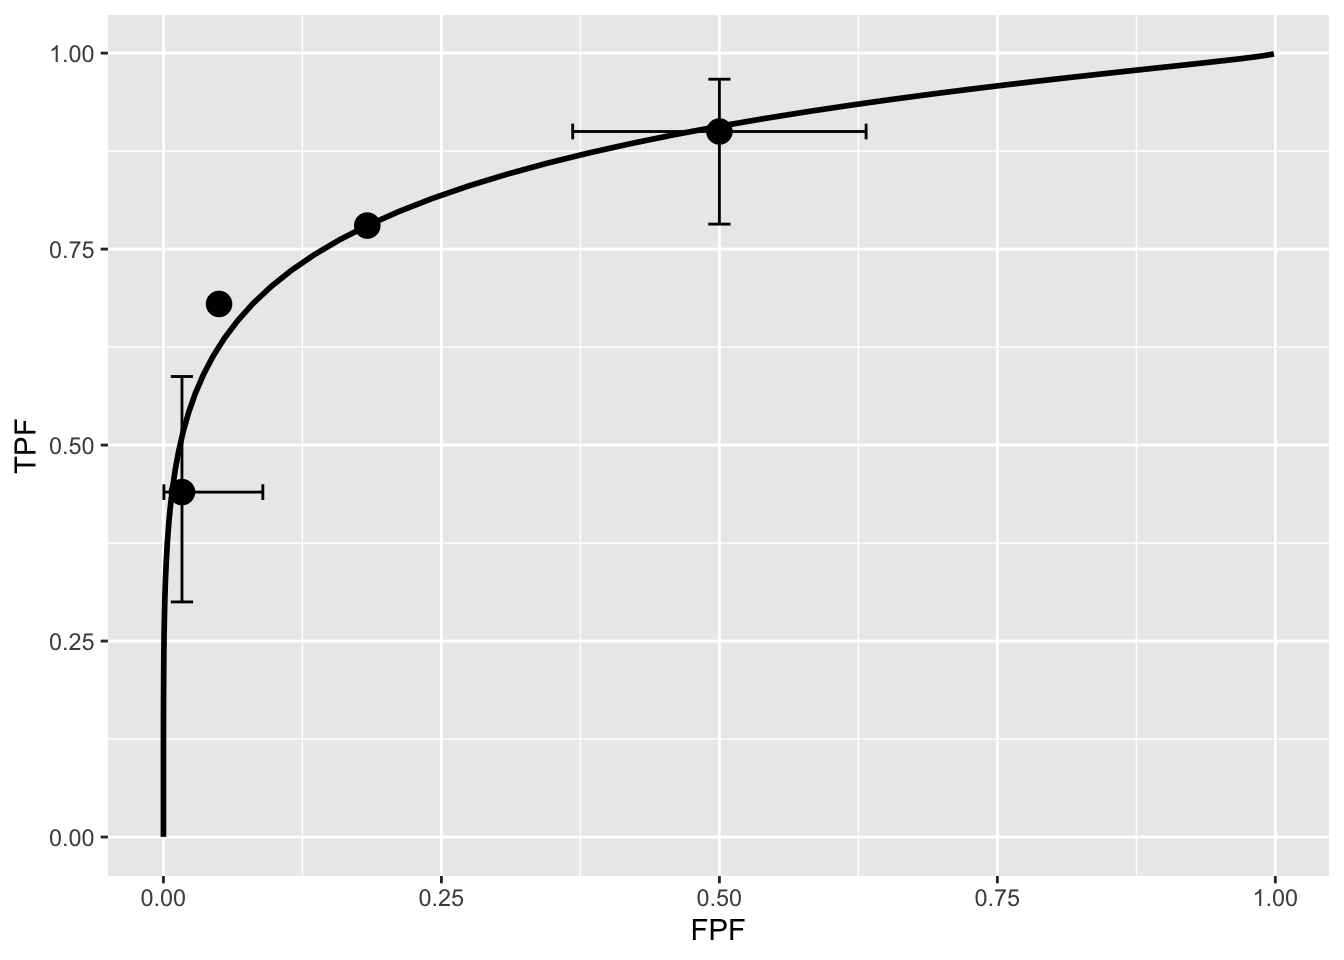
\includegraphics{06-binormal-model_files/figure-latex/binormal-model-fit-1.pdf}
\caption{\label{fig:binormal-model-fit}Operating points and fitted binormal ROC curve. The fitting values are \(a = 1.3205\) and \(b = 0.6075\). Confidence intervals are shown for the lowest and uppermost non-trivial points.}
\end{figure}

Note the usage of the \texttt{RJafroc} package \citep{R-RJafroc}. Specifically, the function \texttt{FitBinormalRoc}. The ratings table is converted to an \texttt{RJafroc} dataset object, followed by application of the fitting function. The results, contained in \texttt{retFit} should be compared to those obtained from the \href{http://www.rad.jhmi.edu/jeng/javarad/roc/JROCFITi.html}{website implementation of ROCFIT}.

\hypertarget{binormal-model-curve-fitting-validation}{%
\subsection{Validating the fit}\label{binormal-model-curve-fitting-validation}}

The above ROC curve is a good visual fit to the observed operating points. Quantification of the validity of the fitting model is accomplished by calculating the Pearson goodness-of-fit test \citep{RN2656}, also known as the chi-square test, which uses the statistic defined by \citep{larsen2005introduction}:

\begin{equation} 
C^2=\sum_{t=1}^{2}\sum_{r=1}^{R}\frac{\left (K_{tr}-\left \langle K_{tr} \right \rangle  \right )^2}{\left \langle K_{tr} \right \rangle}\\
K_{tr} \geq 5
\label{eq:binormal-modelGoodnessFit}
\end{equation}

The expected values are given by:

\begin{equation}
\begin{split}
\left \langle K_{1r} \right \rangle &=K_1\left ( \Phi\left ( \zeta_{r+1} \right ) - \Phi\left ( \zeta_r \right )  \right ) \\
\left \langle K_{2r} \right \rangle &=K_2\left ( \Phi\left ( a\zeta_{r+1}-b \right ) - \Phi\left ( a\zeta_r - b\right )  \right )
\end{split}
\label{eq:binormal-modelGoodnessFitExpVals}
\end{equation}

These expressions should make sense: the difference between the two CDF functions is the probability of a count in the specified bin, and multiplication by the total number of relevant cases should yield the expected counts (a non-integer).

It can be shown that under the null hypothesis that the assumed probability distribution functions for the counts equals the true probability distributions, i.e., the model is valid, the statistic \(C^2\) is distributed as:

\begin{equation} 
C^2\sim \chi_{df}^{2}
\label{eq:binormal-modelGoodnessFitDistr}
\end{equation}

Here \(C^2\sim \chi_{df}^{2}\) is the chi-square distribution with degrees of freedom \emph{df} defined by:

\begin{equation} 
df=\left ( R-1 \right )+\left ( R-1 \right )-\left (2+ R-1 \right )=\left ( R-3 \right )
\label{eq:binormal-modelGoodnessFitdf}
\end{equation}

The right hand side of the above equation has been written in an expansive form to illustrate the general rule: for \(R\) non-diseased cells in the ratings table, the degree of freedom is \(R-1\): this is because when all but one cells are specified, the last is determined, because they must sum to \(K_1\) . Similarly, the degree of freedom for the diseased cells is also \(R-1\). Last, we need to subtract the number of free parameters in the model, which is \((2+R-1)\), i.e., the \(a,b\) parameters and the \(R-1\) thresholds. It is evident that if \(R = 3\) then \(df = 0\). In this situation, there are only two non-trivial operating points and the straight-line fit shown will pass through both of them. With two basic parameters, fitting two points is trivial, and goodness of fit cannot be calculated.

Under the null hypothesis (i.e., model is valid) \(C^2\) is distributed as \(\chi_{df}^{2}\). Therefore, one computes the probability that this statistic is larger than the observed value, called the \emph{p-value}. If this probability is very small, that means that the deviations of the observed values of the cell counts from the expected values are so large that it is unlikely that the model is correct. The degree of unlikeliness is quantified by the p-value. Poor fits lead to small p values.

At the 5\% significance level, one concludes that the fit is not good if \(p < 0.05\). In practice one occasionally accepts smaller values of \(p\), \(p > 0.001\) before completely abandoning a model. It is known that adoption of a stricter criterion, e.g., \(p > 0.05\), can occasionally lead to rejection of a retrospectively valid model \citep{RN300}.

\hypertarget{estimating-the-covariance-matrix}{%
\subsection{Estimating the covariance matrix}\label{estimating-the-covariance-matrix}}

TBA See book chapter 6.4.3. This is implemented in \texttt{RJafroc.}

\hypertarget{estimating-the-variance-of-az}{%
\subsection{Estimating the variance of Az}\label{estimating-the-variance-of-az}}

TBA See book chapter 6.4.4. This is implemented in \texttt{RJafroc}.

\hypertarget{binormal-model-improper-curves}{%
\section{Appendix: Improper ROCs}\label{binormal-model-improper-curves}}

The binormal model has two parameters. The \(a\) parameter is the separation of the two distributions. The diseased case distribution has unit standard deviation. The non-diseased case distribution has standard deviation \(b\). Binormal model fits invariably lead to ROC curves that inappropriately cross the chance diagonal, i.e., it predicts a region of the curve where performance is worse than chance even for expert observers. Such curves are termed \emph{improper}. This occurs whenever \(b \ne 1\).

The following code illustrates improper curves predicted by the binormal model.

\begin{Shaded}
\begin{Highlighting}[]
\NormalTok{  aArray }\OtherTok{\textless{}{-}} \FunctionTok{c}\NormalTok{(}\FloatTok{0.7}\NormalTok{, }\FloatTok{0.7}\NormalTok{, }\FloatTok{1.5}\NormalTok{, }\DecValTok{2}\NormalTok{)}
\NormalTok{  bArray }\OtherTok{\textless{}{-}} \FunctionTok{c}\NormalTok{(}\FloatTok{0.5}\NormalTok{, }\FloatTok{1.5}\NormalTok{, }\FloatTok{0.5}\NormalTok{, }\FloatTok{0.5}\NormalTok{)}
\NormalTok{  chance\_diag }\OtherTok{\textless{}{-}} \FunctionTok{data.frame}\NormalTok{(}\AttributeTok{x =} \FunctionTok{c}\NormalTok{(}\DecValTok{0}\NormalTok{,}\DecValTok{1}\NormalTok{), }\AttributeTok{y =} \FunctionTok{c}\NormalTok{(}\DecValTok{0}\NormalTok{,}\DecValTok{1}\NormalTok{))}
\NormalTok{  p }\OtherTok{\textless{}{-}} \FunctionTok{PlotBinormalFit}\NormalTok{(aArray, bArray) }\SpecialCharTok{+}
    \FunctionTok{scale\_x\_continuous}\NormalTok{(}\AttributeTok{expand =} \FunctionTok{c}\NormalTok{(}\DecValTok{0}\NormalTok{, }\DecValTok{0}\NormalTok{)) }\SpecialCharTok{+} 
    \FunctionTok{scale\_y\_continuous}\NormalTok{(}\AttributeTok{expand =} \FunctionTok{c}\NormalTok{(}\DecValTok{0}\NormalTok{, }\DecValTok{0}\NormalTok{)) }\SpecialCharTok{+}
    \FunctionTok{theme}\NormalTok{(}\AttributeTok{legend.position =} \FunctionTok{c}\NormalTok{(}\FloatTok{0.85}\NormalTok{, }\FloatTok{0.2}\NormalTok{))}
\NormalTok{p }\OtherTok{\textless{}{-}}\NormalTok{ p }\SpecialCharTok{+} \FunctionTok{geom\_line}\NormalTok{(}\AttributeTok{data =}\NormalTok{ chance\_diag, }\FunctionTok{aes}\NormalTok{(}\AttributeTok{x =}\NormalTok{ x, }\AttributeTok{y =}\NormalTok{ y), }\AttributeTok{linetype=}\StringTok{"dotted"}\NormalTok{)}
\end{Highlighting}
\end{Shaded}

\begin{figure}
\centering
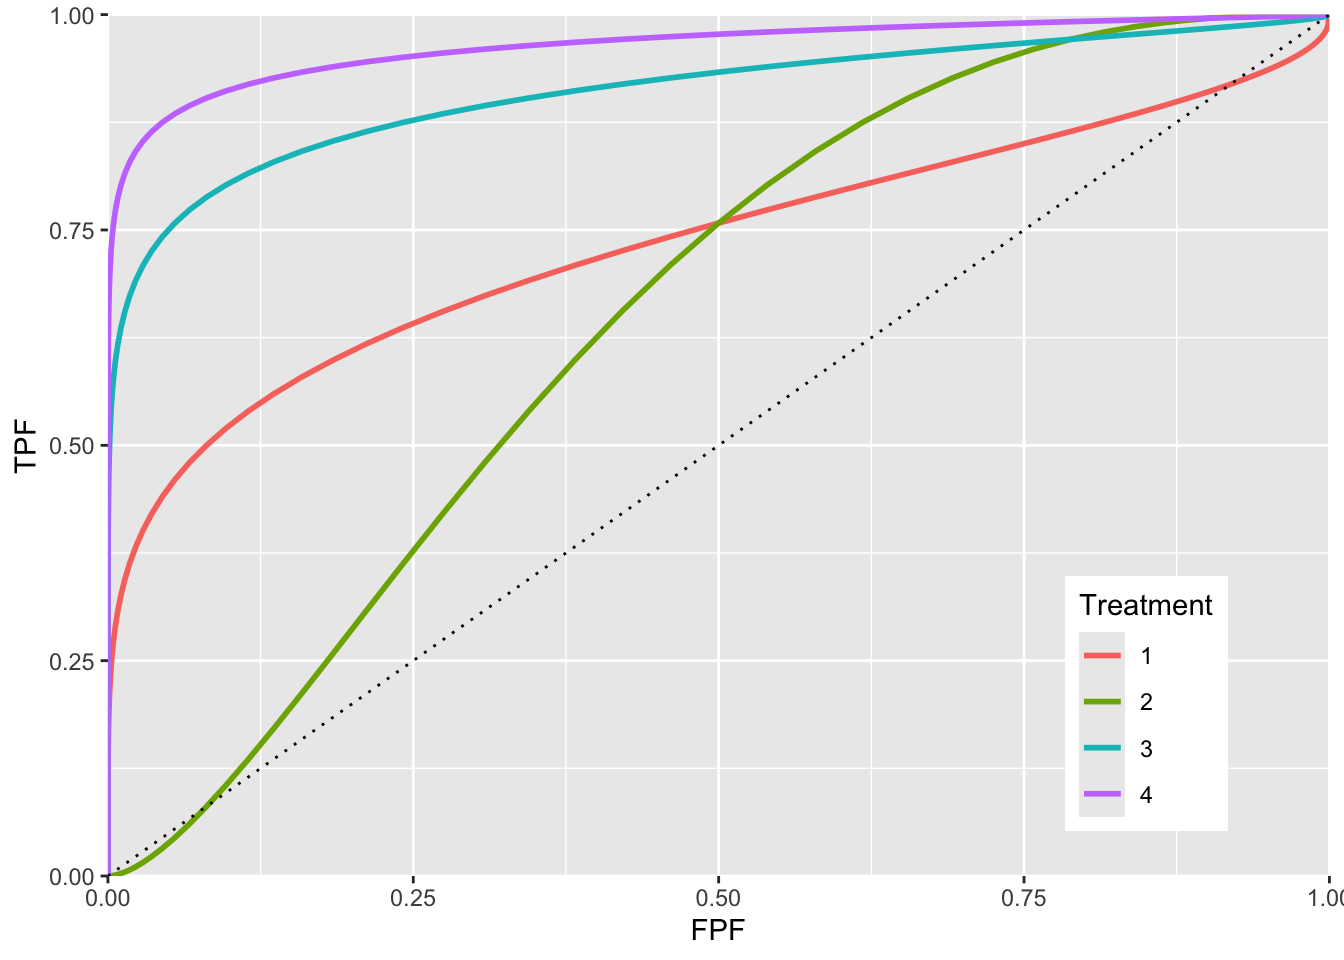
\includegraphics{06-binormal-model_files/figure-latex/improper-roc-1.pdf}
\caption{\label{fig:improper-roc}ROC curves for different parameters. The curve 1 corresponds to \(a = 0.7, b = 0.5\) and shows the clearest example of chance line crossing. Curve 2 corresponds to \(a = 0.7, b = 1.5\) and it shows chance line crossing near the origin. Curve 3 line corresponds to \(a = 1.5, b = 0.5\). Curve 4 corresponds to \(a = 2, b = 0.5\). All curves exhibit chance line crossings even though they may not be clearly evident.}
\end{figure}

The red plot (curve 1) is the clearest example of an improper ROC. The chance line crossing near the upper right corner, around (0.919,0.919) and the fact that the ROC curve must eventually reach (1, 1) implies that the curve must turn upwards as one approaches (1, 1) thereby displaying a ``hook''. Whenever \(b \ne 1\) the hook is there regardless of whether it is easily visible or not. If \(b < 1\) the hook is near the upper right corner. If \(b > 1\) the hook is near the origin (see green line, curve 2, corresponding to \(a = 0.7, b = 1.5\)). With increasing \(a\) the hook is less prominent (see blue line corresponding to \(a = 1.5, b = 0.5\) and purple line corresponding to \(a = 2, b = 0.5\). But it is there.

\hypertarget{reason-for-improper-rocs}{%
\subsection{Reason for improper ROCs}\label{reason-for-improper-rocs}}

The reason for the ``hook'' becomes apparent upon examination of the pdfs.

\begin{figure}
\centering
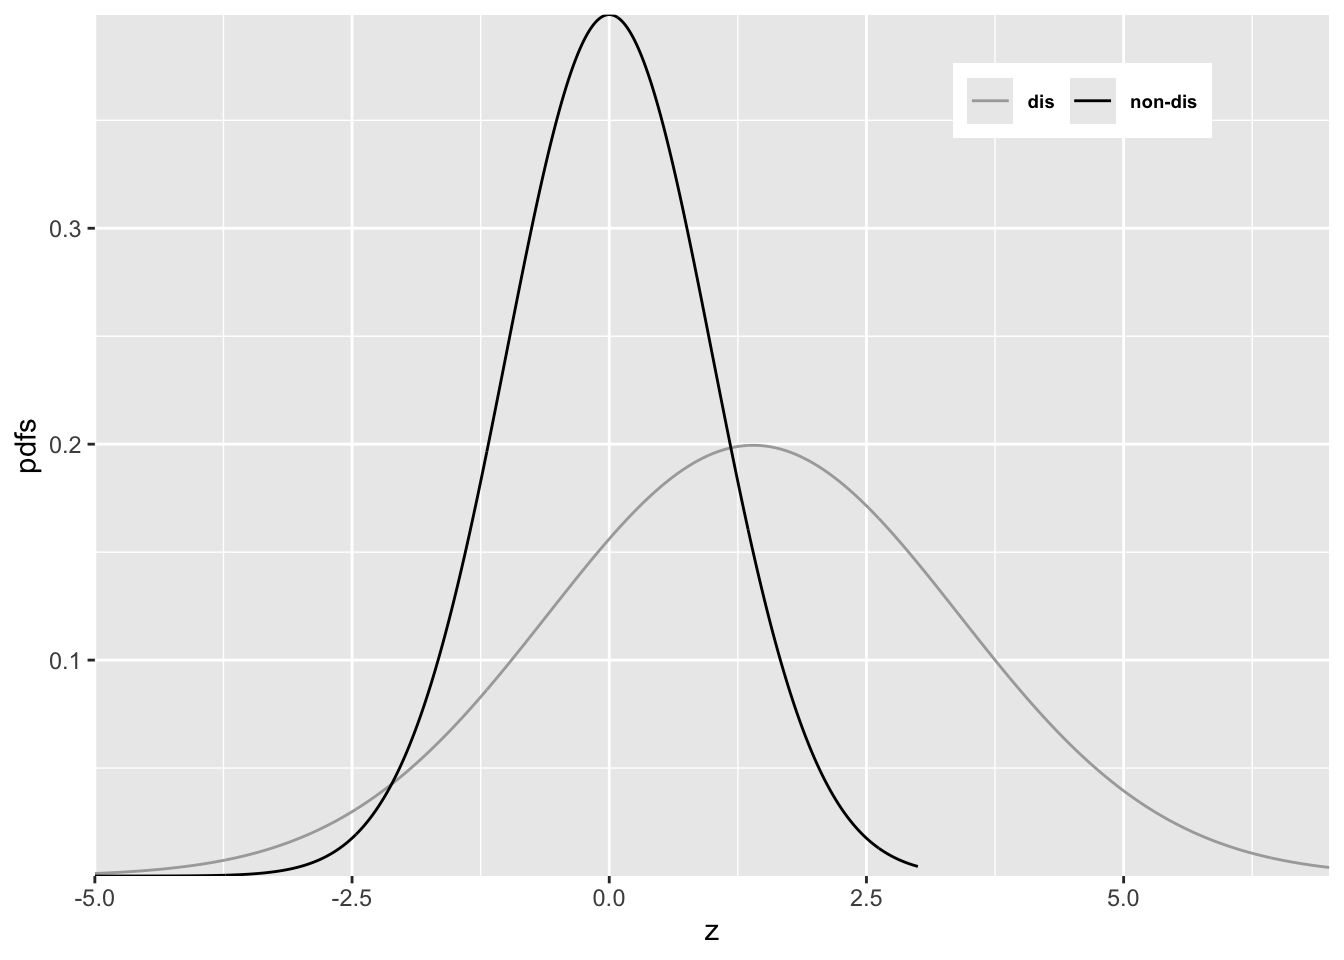
\includegraphics{06-binormal-model_files/figure-latex/improper-roc-reason-1.pdf}
\caption{\label{fig:improper-roc-reason}Reason for improper ROC}
\end{figure}

In Figure \ref{fig:improper-roc-reason} \(a = 0.7\) and \(b = 0.5\). Since \(b < 1\) the diseased pdf is broader and has a lower peak (since the integral under each distribution is unity) than the non-diseased pdf. Starting from the extreme right and then sliding an imaginary threshold to the left one sees that initially, just below \(z = 7\), the diseased distribution starts contributing while the non-diseased distribution is not contributing, causing the ROC to start with infinite slope near the origin (because TPF is increasing while FPF is not). Around \(z = 2.5\) the non-diseased distribution starts contributing, causing the ROC slope to decrease (since FPF is now increasing). Around \(z = -3\) almost all of the non-diseased distribution has contributed which means FPF is near unity, but since not all of the broader diseased distribution has contributed TPF is less than unity. Here is a region where \(TPF < FPF\), meaning that the operating point is below the chance diagonal. As the threshold is lowered further, TPF continues to increase, as the rest of the diseased distribution contributes while FPF stays almost constant at unity. In this region, the ROC curve is approaching the upper right corner with almost infinite slope (because TPF is increasing but FPF is not).

Usually the hook is not readily visible. For example, in Fig. \ref{fig:binormal-model-fit} one would have to ``zoom-in'' on the upper right corner to see. An example from a clinical study is Fig. 1 in \citep{pisano2005diagnostic} where each of the film modality ROC curves show the ``hook''. Ways of fitting proper ROC curves are described in Chapter \ref{proper-roc-models}.

One reason for for \(b < 1\), namely location uncertainty, follows from the Radiological Search Model (RSM) presented in \texttt{RJafrocFrocBook}. If the location of the lesion is unknown to the observer, then z-samples from diseased cases are of two types: samples from lesion localizations centered at \(\mu\) or samples from non-lesion localizations centered at 0. The resulting mixture-distribution will have larger variance than samples from non-diseased regions centered at 0 occurring on non-diseased cases. The mixing need not be restricted to location uncertainty. Even is location is known, if the lesions are non-homogenous (e.g., they contain a range of contrasts or sizes) then a similar mixture-distribution induced broadening is expected. The contaminated binormal model (CBM) -- see Chapter \texttt{TempComment\ \textbackslash{}@ref(proper-roc-models)} -- also predicts that the diseased distribution is wider than the non-diseased one.

\hypertarget{binormal-model-degeneracy}{%
\section{Degenerate datasets}\label{binormal-model-degeneracy}}

The unphysical nature of the ``hook'' is not the only reason for seeking alternate ROC models. The binormal model is also highly susceptible to degeneracy problems.

\begin{quote}
Metz defined binormal degenerate data sets as those that result in exact-fit binormal ROC curves of inappropriate shape consisting of a series of horizontal and/or vertical line segments in which the ROC ``curve'' crosses the chance line.
\end{quote}

\hypertarget{binormal-model-understanding-degenerate-datasets}{%
\subsection{Understanding degenerate datasets}\label{binormal-model-understanding-degenerate-datasets}}

To understand this, consider that the non-diseased distribution pdf is a Dirac delta function centered at zero (this function integrates to unity) and the unit variance diseased distribution is centered at 0.6744898. In other words this model is characterized by \(a = 0.6744898\) and \(b = 0\). As the threshold \(\zeta\) is moved leftward starting from the far right TPF will increase but \(\text{FPF}=0\) until \(\zeta\) reaches zero. Just before reaching this value the coordinates of the ROC operating point are (0, 0.75). The 0.75 is due to the fact that \(z = 0\) is -0.6744898 units relative to the center of the diseased distribution, so the area under the diseased distribution to the left of \(z = 0\) is \texttt{pnorm(-0.6744898)}, i.e., 0.250. Since \texttt{pnorm} is the probability to the left of the threshold, TPF is its complement, namely \texttt{1-pnorm(-0.6744898)}, i.e., 0.750000016.

As the threshold crosses the delta function FPF jumps from 0 to 1 but TPF stays constant. The operating point has jumped from (0, 0.75) to (1, 0.75). When the threshold is reduced further, the operating point moves up vertically along the right side of the ROC plot, until the threshold is so small that virtually all of diseased distribution exceeds it and the operating point reaches (1, 1). The ROC curve is illustrated in Fig. \ref{fig:binormal-model-degeneracy-fig} panel A, which is an extreme example of an ROC curve with a ``hook''. Since the fit passes through the sole operating point provided by the observer, i.e., (0,0.75), it is an exact fit to the operating point.

\hypertarget{binormal-model-exact-fit-not-unique}{%
\subsection{The exact fit is not unique}\label{binormal-model-exact-fit-not-unique}}

Given only one observed operating point (0, 0.75) the preceding fit is not unique. If the diseased distribution is shifted appropriately to the right, by varying \(a\), see below, then the ROC curve will be the vertical line segment from the origin to (0, 0.9) followed by a horizontal line segment to (1, 0.9) and a vertical line segment to (1, 1), see Fig. \ref{fig:binormal-model-degeneracy-fig} panel B. If the diseased distribution is shifted well to the right, i.e., \(a\) is very large, then the ROC curve will be the vertical line segment from the origin to (0,1) followed by the horizontal line segment to (1, 1) as in panel C.

\begin{figure}
\centering
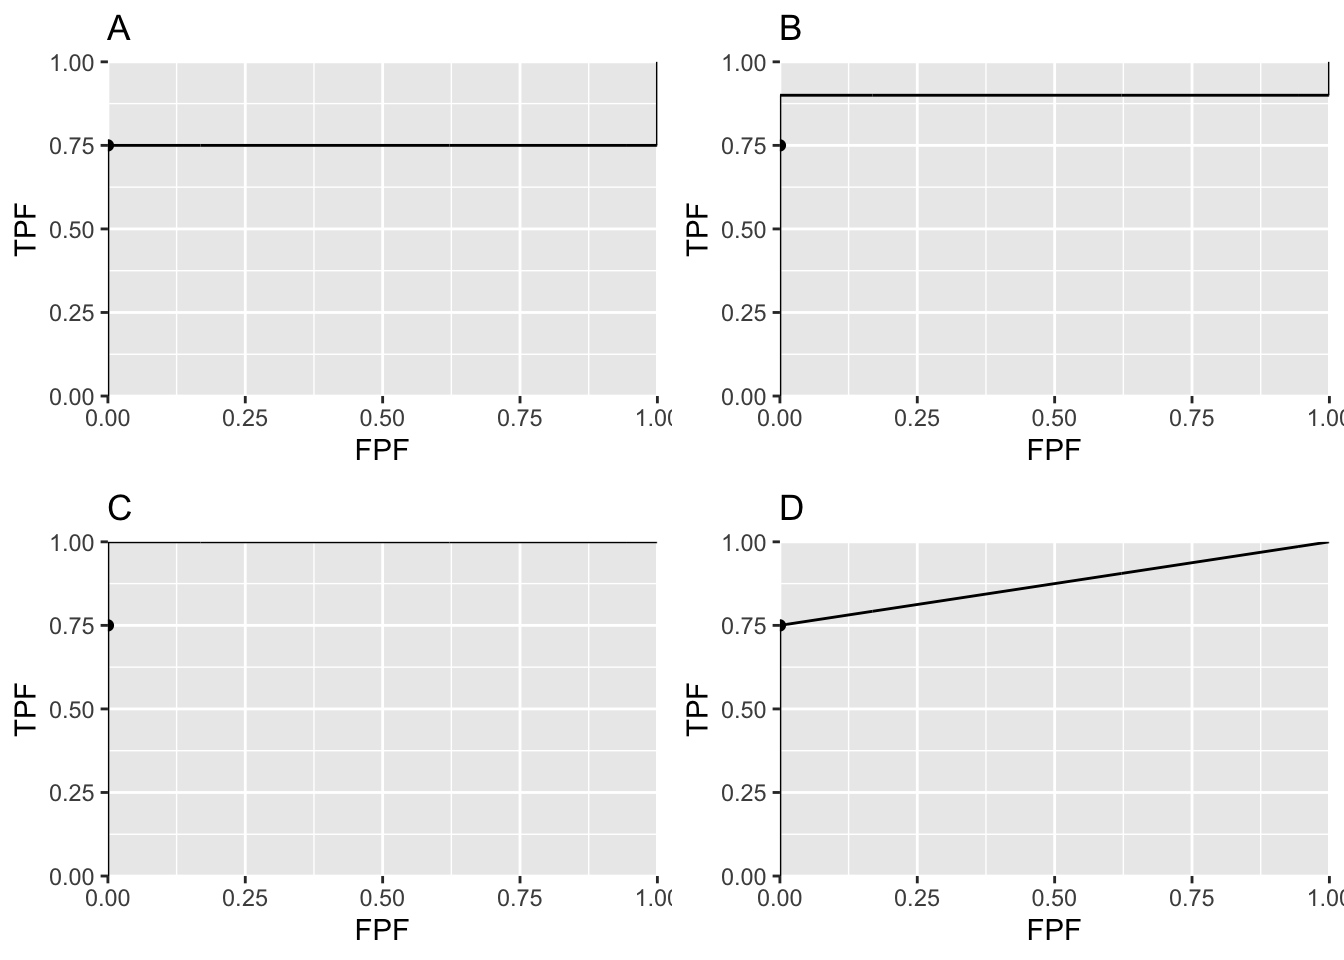
\includegraphics{06-binormal-model_files/figure-latex/binormal-model-degeneracy-fig-1.pdf}
\caption{\label{fig:binormal-model-degeneracy-fig}Panels A, B and C illustrate that the exact fit is not unique. Panel D illustrates a reasonable unique fit to the data.}
\end{figure}

Panels A, B and C in Fig. \ref{fig:binormal-model-degeneracy-fig} represent exact fits to the observed operating point with \(b = 0\) and different values of \(a\). None of them is reasonable. Panel D is discussed below.

\hypertarget{binormal-model-spread-ratings}{%
\subsection{On instructing an observer to ``spread their ratings''}\label{binormal-model-spread-ratings}}

\begin{quote}
Degeneracy occurs if the observer does not provide any interior operating points. Perhaps one has a non-cooperating observer who is not heeding the instructions to \emph{spread the ratings, use all the bins}. The observer could in fact be cooperating fully and still be unable to provide any interior data points.
\end{quote}

\begin{quote}
Consider 100 diseased cases consisting of 75 easy cases and 25 difficult cases and 100 non-diseased cases of varying degrees of difficulty but less suspicious than the ``five'' category. The observer is expected to rate the 75 easy diseased cases as ``fives'' and the remaining cases as less than ``fives'' yielding the operating point (0, 0.75). No amount of coaxing to ``spread their ratings'' is going to convince the observer to rate with ``twos'', ``threes'' and ``fours'' any of the 75 easy diseased cases. If the cases are obviously diseased, and that is what is meant by easy diseased cases, they are supposed to be rated fives, i.e., definitely diseased. Forcing them to rate some of them as ``probably diseased'' or ``possibly diseased'' would be like altering the reading paradigm to fit the convenience of the researcher, never a good idea.
\end{quote}

\hypertarget{binormal-model-reasonable-fit}{%
\subsection{A reasonable fit to the degenerate dataset}\label{binormal-model-reasonable-fit}}

\begin{quote}
Theorem: given an observed operating point the line connecting that point to (1, 1) represents a lower bound on achievable performance by the observer.
\end{quote}

The observer achieves the lower bound by guessing to classify the remaining cases, i.e., those not contributing to the observed operating point. This is how it works: having rated the 75 easy diseased cases as ``fives'' and the rest of the cases in lower bins the guessing observer randomly rates 1/5th of the remaining cases in the ``four'' bin. This would add 5 diseased cases (25/5) and 20 non-diseased cases (100/5) in the ``four'' bin yielding the interior point (0.20, 0.80). If the observer randomly rates 2/5th of the cases to the ``four'' bin rating category one obtains the interior point (0.40, 0.85). By simply increasing the fraction of cases that are randomly rated ``fours'' the observer can move the operating point along the straight line connecting (0, 0.75) and (1, 1), as in plot D in Fig. \ref{fig:binormal-model-degeneracy-fig}. Since it involves guessing this must represent a lower bound on performance.

\begin{quote}
The lowest possible performance yields a unique ROC curve: any higher ROC curve would not be unique.
\end{quote}

\hypertarget{binormal-model-references}{%
\section{Chapter References}\label{binormal-model-references}}

\hypertarget{part-advanced-topics}{%
\part*{Advanced topics}\label{part-advanced-topics}}
\addcontentsline{toc}{part}{Advanced topics}

\hypertarget{proper-roc-models}{%
\chapter{Proper ROC models}\label{proper-roc-models}}

\hypertarget{proper-roc-models-how-much-finished}\label{proper-roc-models-how-much-finished}}

\hypertarget{proper-roc-models-introduction}{%
\section{Introduction}\label{proper-roc-models-introduction}}

The binormal model has been widely used to fit ROC datasets in a wide range of applications not limited to medical imaging. However, binormal model fits almost invariably lead to ROC curves that inappropriately cross the chance diagonal leading to a prediction of a region of the ROC curve where performance is worse than chance even for expert observers. By convention, such curves are termed ``improper''. A chance line crossing near the upper right corner of the ROC plot occurs when \(b < 1\) and near the origin if \(b > 1\).

\begin{quote}
Since \(b\) is a continuous-variable parameter there is zero probability that an estimate of \(b\) will be exactly equal to one, the only condition under which there is no ``hook''. Therefore, every fitted binormal model ROC curve is ``improper''.
\end{quote}

The improper behavior is often not readily visible. One may need to ``zoom-in'' on the upper-right corner to see it. Any fit that predicts worse than chance level performance anywhere on the ROC plot, visible or not, is scientifically indefensible. Much effort has gone into developing models that always predict proper ROC curves, i.e., those that do not cross the chance diagonal. These are called ``proper'' ROC curves (some of literature uses the quotes and some does not). There are at least four methods for fitting proper ROC curves, and these are listed in reverse chronological order.

\begin{itemize}
\item
  The most recent (2016) one \citep{chakraborty2011estimating, chakraborty2012inverse} is based on the radiological search model (RSM) and is implemented in the \texttt{RJafroc} package.
\item
  A method \citep{dorfman2000contaminated1, dorfman2000contaminated2, dorfman2000contaminated3} based on the contaminated binormal model (CBM), available as part of DBM-MRMC software from a University of Iowa website and also implemented in the \texttt{RJafroc} package.
\item
  The binormal model-based proper ROC fitting algorithm \citep{metz1999proper, pan1997proper} developed by Metz and Pan implemented in PROPROC software available as part of DBM-MRMC software.
\item
  The bigamma model \citep{dorfman1997proper} fitting algorithm for which no software currently exists but is fairly easy to implement.
\item
  LROCFIT, based on the location ROC (LROC) paradigm \citep{swensson1996unified}, which also predicts proper ROC curves, but the data has to be acquired according to the LROC paradigm while all of the other methods described in this chapter work with ROC data (no localization information).
\end{itemize}

A related issue is data degeneracy that occurs when a reader fails to provide an interior ROC point. The binormal model does not yield reasonable fits to such data and the researcher has no option but to discard the data or use the empirical AUC.

\begin{quote}
To understand how proper ROCs can be generated we need to understand a quantity called the likelihood ratio and the fact that slope of the ROC curve always equals the likelihood ratio, independent of parametric assumptions.
\end{quote}

\hypertarget{proper-roc-models-likelihood-ratio-theorem1}{%
\section{ROC slope equals likelihood ratio}\label{proper-roc-models-likelihood-ratio-theorem1}}

According to the binormal model:

\begin{equation} 
\left.\begin{aligned}
\text{FPF}&=\Phi\left( -z \right)\\
\text{TPF}&=\Phi\left( a-bz \right)
\end{aligned}
\right\}
\label{eq:proper-roc-models-binormal-model}
\end{equation}

The slope \(m\left( z|a,b \right)\) of the ROC curve is:

\begin{equation} 
\left.\begin{aligned}
m\left( z|a,b \right)&=\frac{\frac{\partial \left( TPF \right)}{\partial z}}{\frac{\partial \left( FPF \right)}{\partial z}}\\ 
&=\frac{b\phi\left( a-bz \right)}{\phi\left( -z \right)}\\ 
&=b\exp\left( -\frac{\left( bz-a \right)^2 - z^2}{2} \right)
\end{aligned}\right\}
\label{eq:proper-roc-models-slope}
\end{equation}

The probability density functions (pdfs) for the binormal model were defined earlier and are reproduced here (N = non-diseased, D = diseased):

\begin{equation} 
\left.\begin{aligned}
\text{pdf}_N\left( z \right) &= \frac{1}{\sqrt{2\pi}}\exp\left( -\frac{z^2}{2} \right) \\
\text{pdf}_D\left( z \right) &= \frac{b}{\sqrt{2\pi}}\exp\left( -\frac{\left( bz-a \right)^2}{2} \right) \\
\end{aligned}\right\}
\label{eq:proper-roc-models-pdfs}
\end{equation}

The likelihood ratio is defined by (the subscript ``BIN'' is for ``binormal model''):

\begin{equation} 
\left.\begin{aligned}
l_{\text{BIN}}\left( z | a,b\right) &\equiv \frac{\text{pdf}_D\left( z \right)}{\text{pdf}_N\left( z \right)} \\
&= b\exp\left( -\frac{\left( bz-a \right)^2 -z^2}{2} \right) \\
\end{aligned}\right\}
\label{eq:proper-roc-models-likelihood-ratio}
\end{equation}

It is seen from Eqn. \eqref{eq:proper-roc-models-slope} and Eqn. \eqref{eq:proper-roc-models-likelihood-ratio} that the likelihood ratio equals the slope of the ROC curve:

\begin{equation} 
l_{\text{BIN}}\left( z | a,b\right) = m\left( z | a,b\right)
\label{eq:proper-roc-models-likelihood-ratio-theorem}
\end{equation}

While illustrated for the binormal model, this theorem is actually independent of any distributional assumptions \citep{Egan1975}. The reason for the name ``likelihood ratio'' is that early researchers in the field used the term ``likelihood function'' for what statisticians now term ``probability density function''. Hence the ratio of two likelihood functions was termed a ``likelihood ratio'' when in fact it is a ratio of two pdfs.

\hypertarget{proper-roc-models-likelihood-ratio-theorem2}{%
\section{The likelihood ratio observer maximizes AUC}\label{proper-roc-models-likelihood-ratio-theorem2}}

An observer who maximizes TPF at each FPF for all values \(0 \le \text{FPF} \le 1\) is called a Neyman-Pearson observer \citep{neyman1933ix}. It can be shown that the Neyman-Pearson observer uses the likelihood ratio as the decision variable \citep{green1966signal}.

\begin{quote}
A consequence is that AUC for a likelihood ratio observer represents an upper limit on performance, and such an observer is called an ``ideal observer''. Moreover use of the likelihood ratio as the decision variable always yields proper ROC curves.
\end{quote}

These statements call for an explanation.

\hypertarget{explanation}{%
\subsection{Explanation}\label{explanation}}

So far the decision rule has been that if the z-sample for a case satisfies \(z \ge \zeta\) the case is diagnosed as diseased and otherwise it is diagnosed as non-diseased.

The likelihood ratio involves a deeper concept. It is assumed that the observer knows the pdfs of non-diseased and diseased cases as functions of z. The observer computes the ratio \(l(z)\) at the observed z-sample. If \(l(z) \ge \lambda\) the case is diagnosed as diseased and otherwise the case is diagnosed as non-diseased. Note the difference:

\begin{itemize}
\item
  Binormal model observer: \(z \ge \zeta\)
\item
  Likelihood ratio observer: \(l(z) \ge \lambda\)
\end{itemize}

A word on notation: when the decision variable was \(z\) I used the corresponding Greek character \(\zeta\) to denote a threshold on the z-axis. Since likelihood ratio is denoted \(l\), the corresponding Greek character is \(\lambda\).

The observer has transformed the decision variable \(z\) to a new variable \(l(z)\) and uses the new variable to make decisions. Varying \(\lambda\) allows the observer to generate the \emph{likelihood ratio ROC curve} which is ``proper''.

If the decision variable \(z\) results in improper ROC curves, as does the z-sample in the binormal model, the transformation will not be monotonic \footnote{For a positive-directed decision variable, as in this book, the term ``monotonic'' is always meant to be ``monotonic increasing''. It is possible for a transformation to be monotonic decreasing, as in \(l = 1/z\).}. If the transformation were monotonic, that would imply that z was already equivalent to the likelihood ratio.

To summarize these concepts the likelihood ratio observer transforms \(z\) to \(l(z)\):

\begin{equation} 
l\left( z \right) \equiv  \frac{\text{pdf}_D\left( z \right)}{\text{pdf}_N\left( z \right)}
\label{eq:proper-roc-models-likelihood-ratio-definition}
\end{equation}

Then the decision variable \(M\left( l\left( z \right) \right)\) will yield a proper ROC curve. Here \(M\left( \right)\) is an arbitrary monotonic increasing function of its argument, i.e.~if \(x_2 > x_1\):

\begin{equation} 
M\left( x_2 \right) \ge M\left( x_1 \right) 
\label{eq:proper-roc-models-definition-monotonic}
\end{equation}

The transformation allows flat portions.

\hypertarget{proper-roc-models-likelihood-ratio-observer}{%
\section{The likelihood ratio observer}\label{proper-roc-models-likelihood-ratio-observer}}

\begin{quote}
An observer using the likelihood ratio or any monotonic transformation of it as the decision variable is termed a likelihood ratio observer.
\end{quote}

In Fig. \ref{fig:proper-roc-models-plots-2} plots A-F, all of which apply to \(a = 0.7\) and \(b = 0.5\), the ordinate is labeled \(\text{lr}\) for likelihood ratio.

\begin{figure}
\centering
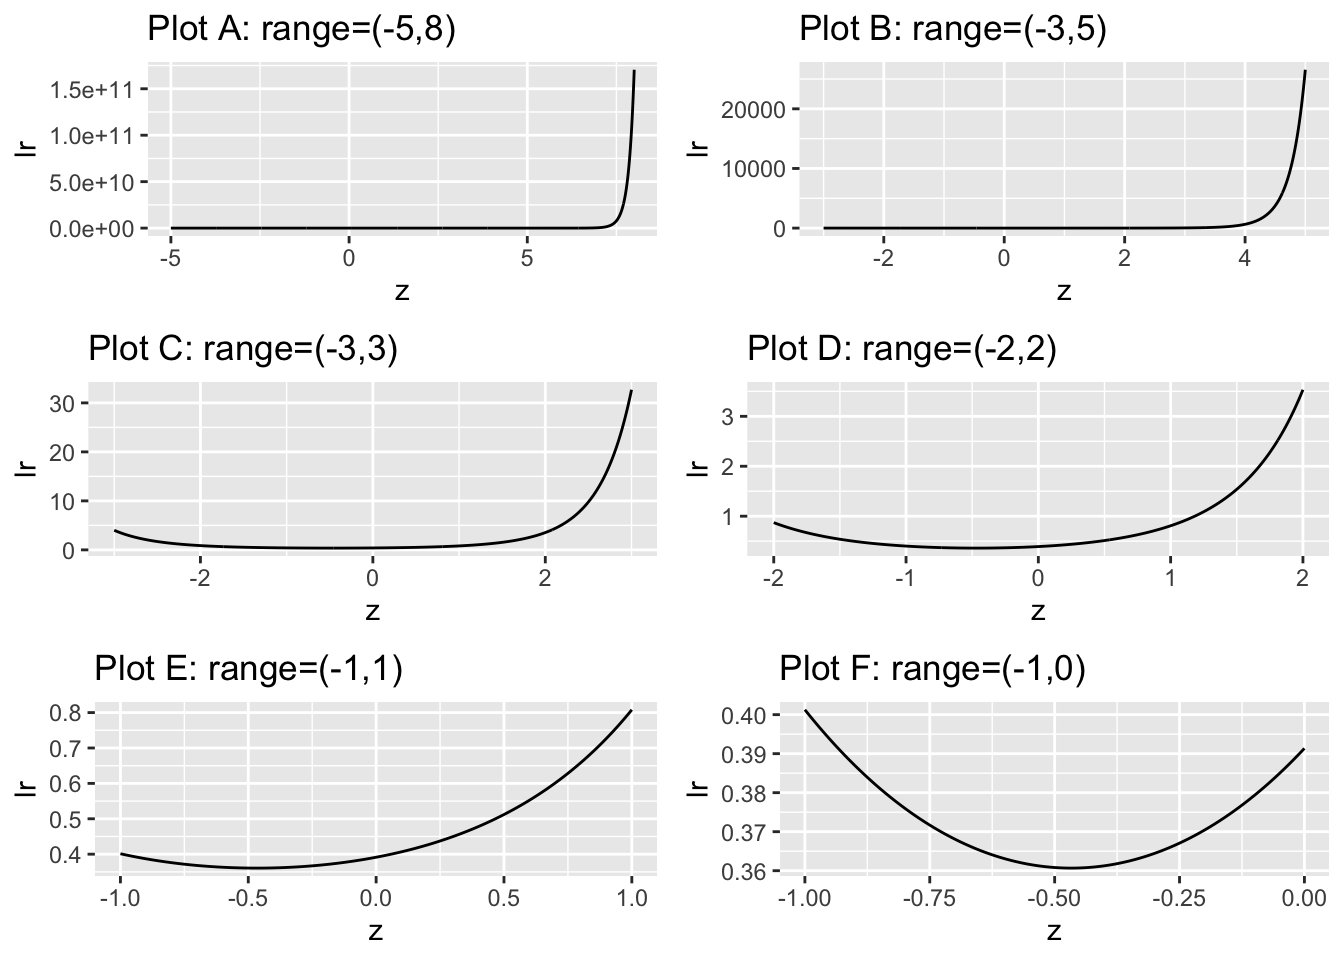
\includegraphics{07-proper-roc-models_files/figure-latex/proper-roc-models-plots-2-1.pdf}
\caption{\label{fig:proper-roc-models-plots-2}These plots of likelihood ratio \(\text{lr}\) of the ROC curves as functions of z for \(a = 0.7, b = 0.5\). They correspond to different ranges along the z-axis, starting with a `birds-eye' view (panel A) and gradually focusing in on the region near the minimum (panel F).}
\end{figure}

Focusing on plot A in Fig. \ref{fig:proper-roc-models-plots-2} in which range of z is -5 to 8, imagine a sliding threshold \(\lambda\) moving down along the ordinate, starting from very high values, \(\approx 1.5 \times 10^{11}\). The decision rule is to diagnose the case as ``diseased'' if \(\text{lr} \ge \lambda\), and otherwise the case is diagnosed as ``non-diseased''. In plot A the likelihood ratio \(\text{lr}\) seems, for all practical purposes, to be monotonically related to z, so on the surface it makes no difference which decision rule is used, that based on \(\text{lr} \ge \lambda\) or that based on \(z \ge \zeta\). The same conclusion is reached for Plot B, which focuses on the range (-3,5). Plot C showing the range (-3,3) reveals the first hint of something different going on, for now the ordinate \(\text{lr}\) is not monotonically related to \(z\) since the \(\text{lr}\) function has a minimum. For \(\text{lr} > \approx 1\) there are two values of \(\zeta\) corresponding to a each value of \(\lambda\). This behavior is amplified in the remaining plots, as one ``homes-in'' on the minimum. Taking the clearest example, plot F, for \(\lambda = 0.37\) the two values are (-0.728, 0.206). These are denoted by \(\zeta_L=-0.728\) and \(\zeta_U=0.206\). The likelihood ratio observer using threshold \(\lambda=0.37\) declares all cases with \(\text{lr} \ge 0.37\) as diseased, and non-diseased otherwise. The corresponding z-sample binormal model observer must declare cases with \(z \ge \zeta_U\) \textbf{and} cases with \(z < \zeta_L\) as diseased, and non-diseased otherwise. The z-sample rule is more complicated and non-intuitive: why should cases with very low z-samples be declared diseased? The reason is that according to the z-sample based model assumed by the observer \textbf{both} very high and very low values of z are consistent with the case being diseased.

\begin{quote}
Since likelihood ratio decreases as one moves down the y-axis in Fig. \ref{fig:proper-roc-models-plots-2}) the slope of the likelihood ratio generated ROC curve decreases monotonically as the operating point moves up the curve. Since likelihood ratio is the ratio of two probabilities, it - and consequently the slope of the ROC - is always non-negative. This rules out chance line crossings and ``hooks''. The likelihood ratio observer always generates a proper ROC curve.
\end{quote}

Recall that the observer needs to know the two pdfs and compute a ratio based on the observed z-sample. Since the pdfs defined above were specific to the binormal model the likelihood ratio observer described above is, more carefully stated, a \emph{binormal-model-based likelihood ratio observer}.

\begin{quote}
It can be shown that the likelihood ratio observer achieves the highest ROC curve (in the Neyman-Pearson sense) and consequently the highest AUC when compared to observers using other decision rules. In this sense the likelihood ratio observer is an \textbf{ideal observer}.
\end{quote}

The observer can use a decision rule that is based on any monotonic increasing transformation of the likelihood ratio and the resulting ROC curve will be identical to that based on the likelihood ratio; the slope of the resulting curve always equals the likelihood ratio (i.e., before the monotonic transformation). For example, the monotonic transformation could yield a variable ranging from -infinity to plus infinity but the slope of the resulting ROC curve will still be that for the likelihood ratio observer prior to the transformation.

Since AUC of the likelihood ratio observer is optimal with respect to other observers using different decision rules or different underlying models of the decision variable, \textbf{the AUC achieved by the likelihood ratio observer is unique regardless of the model used to fit the proper ROC curve.} The shapes of the predicted proper ROC curves could be model dependent and differ from each other but the AUCs will all be the same. This is demonstrated in book Chapter TBA 18 for RSM, PROPROC and CBM models fitted to a large number of datasets.

\hypertarget{proper-roc-models-proproc}{%
\section{PROPROC}\label{proper-roc-models-proproc}}

An algorithm \citep{metz1999proper}, based on the observer using the binormal model likelihood ratio, has been implemented. The software is called PROPROC, for proper ROC. \footnote{The 1999 publication is a difficult read but well worth it for deeper understanding.}

\hypertarget{proper-roc-models-proproc-formulae}{%
\subsection{PROPROC formulae}\label{proper-roc-models-proproc-formulae}}

The method uses two parameters \(c,d_a\) defined as follows:

\begin{equation} 
\left.\begin{aligned}
c &= \frac{b-1}{b+1} \\
d_a &= \frac{\sqrt{2}a}{1+b^2} \\
\end{aligned}\right\}
\label{eq:proper-roc-models-proproc-parameters}
\end{equation}

Allowed values of the parameters are as follows:

\begin{equation} 
\left.\begin{aligned}
& -1 < c < 1 \\
& 0 < d_a < \infty \\
\end{aligned}\right\}
\label{eq:proper-roc-models-proproc-parameter-ranges}
\end{equation}

Eqn. \eqref{eq:proper-roc-models-proproc-parameters} can be solved for the \(a,b\) parameters as functions of the \(c.d_a\) parameters:

\begin{equation} 
\left.\begin{aligned}
a &= \frac{d_a}{\sqrt{2}}\sqrt{1+{{\left( \frac{c+1}{c-1} \right)^2}}} \\
b &= -\frac{c+1}{c-1} \\
\end{aligned}\right\}
\label{eq:proper-roc-models-proproc-parameters-transform}
\end{equation}

Since \(b < 1\) with most clinical datasets, one expects to find \(c < 0\). The proper ROC curve is defined by \citep{metz1999proper} (the threshold variable \(v\), which is the PROPROC analog of \(\zeta\), is defined below):

\begin{equation} 
\left.\begin{aligned}
FPF\left( v \right) &= \Phi\left( -\left( 1-c \right)v -\frac{d_a}{2}\sqrt{1+c^2}  \right) \\ 
&+\Phi\left( -\left( 1-c \right)v +\frac{d_a}{2c}\sqrt{1+c^2} \right)  -H(c) \\
TPF\left( v \right) &= \Phi\left( -\left( 1+c \right)v +\frac{d_a}{2}\sqrt{1+c^2}  \right)  \\ &+\Phi\left( -\left( 1+c \right)v +\frac{d_a}{2c}\sqrt{1+c^2} \right)  -H(c) \\
\end{aligned}\right\}
\label{eq:proper-roc-models-v-range}
\end{equation}

The (Heaviside) step function \(H(x)\) is defined by:

\begin{equation} 
\left.\begin{aligned}
H\left( x < 0 \right) &= 0 \\
H\left( x > 0 \right) &= 1 \\
\end{aligned}\right\}
\label{eq:proper-roc-models-heaviside}
\end{equation}

The function is discontinuous, but its value at \(x = 0\) is irrelevant because \(c = 0\) implies \(b = 1\), in which case the equal variance binormal model applies, which predicts proper ROCs.

Depending on the value of \(c\) the threshold variable \(v\) in Eqn. \eqref{eq:proper-roc-models-v-range} has different ranges:

\begin{equation} 
\left.\begin{aligned}
\begin{matrix}
\frac{d_a}{4c}\sqrt{1+c^2} \le v \le \infty & \text{if} & c<0 
\end{matrix}\\
\begin{matrix}
-\infty \le v \le \infty & \text{if} & c=0 
\end{matrix}\\
\begin{matrix}
-\infty \le v \le\frac{d_a}{4c}\sqrt{1+c^2} \le v & \text{if} & c<0 
\end{matrix}\\
\\
\end{aligned}\right\}
\label{eq:proper-roc-models-limits-v}
\end{equation}

PROPROC software implements a maximum likelihood method to estimate the \(c, d_a\) parameters from ratings data. The 1999 publication \citep{metz1999proper} states, without proof, that the area under the proper ROC is give by:

\begin{equation} 
A_{\text{prop}}=\Phi\left( \frac{d_a}{\sqrt{2}} \right) + 2F\left\{-\frac{d_a}{\sqrt{2}},0;-\frac{1-c^2}{1+c^2}  \right\}
\label{eq:proper-roc-models-metz-36}
\end{equation}

Here \(F(X,Y;\rho)\) is the bivariate standard-normal (i.e., zero means and unit variances) cumulative distribution function (CDF) with correlation coefficient \(\rho\). In the notation of book Chapter 21:

\begin{equation} 
F\left( X,Y;\rho \right)=\int_{x=-\infty}^{X}
\int_{y=-\infty}^{Y}
dx dy ~ ~  f\left( 
\left( \begin{matrix}
x \\
y
\end{matrix}
 \right) \bigg\rvert
\left( \begin{matrix}
0 \\
0
\end{matrix}  \right),
\left( \begin{matrix}
1 & \rho \\
\rho & 1
\end{matrix} \right)
\right)
\label{eq:proper-roc-models-def-bivariate-cdf}
\end{equation}

Here \(f\) is the pdf of a standard-normal bivariate distribution with correlation \(\rho\), i.e., the mean is the zero column vector of length 2 and the 2 x 2 covariance matrix has ones along the diagonal and \(\rho\) along the off-diagonal.

The first term in Eqn. \eqref{eq:proper-roc-models-metz-36} is equal to the area under the binormal model ROC curve Eqn. \eqref{eq:binormal-model-ab-2az}. Therefore,

\begin{equation} 
A_{\text{prop}}=A_z+2F\left( -\frac{d_a}{\sqrt{2}},0;-\frac{1-c^2}{1+c^2} \right)
\label{eq:proper-roc-models-area-proproc2}
\end{equation}

Since F (a CDF, which is a probability) is non-negative,

\begin{equation} 
A_{\text{prop}}\ge A_z
\label{eq:proper-roc-models-area-proproc-az-inequality}
\end{equation}

This reinforces the result stated earlier.

\hypertarget{proper-roc-models-proproc-code}{%
\subsection{PROPROC code implementation}\label{proper-roc-models-proproc-code}}

Here is the code to generate PROPROC ROC curve and slope plots.

\begin{Shaded}
\begin{Highlighting}[numbers=left,,]

\NormalTok{c1Arr }\OtherTok{\textless{}{-}}   \FunctionTok{c}\NormalTok{(}\SpecialCharTok{{-}}\FloatTok{0.1322804}\NormalTok{, }\FloatTok{0.2225588}\NormalTok{)}
\NormalTok{daArr  }\OtherTok{\textless{}{-}}  \FunctionTok{c}\NormalTok{(}\FloatTok{1.197239}\NormalTok{,}\FloatTok{1.740157}\NormalTok{)}
\NormalTok{plotRoc }\OtherTok{\textless{}{-}} \FunctionTok{list}\NormalTok{()}
\NormalTok{plotSlope }\OtherTok{\textless{}{-}} \FunctionTok{list}\NormalTok{()}

\NormalTok{npts }\OtherTok{\textless{}{-}}  \DecValTok{10000}
\ControlFlowTok{for}\NormalTok{ (i }\ControlFlowTok{in} \DecValTok{1}\SpecialCharTok{:}\DecValTok{2}\NormalTok{)}
\NormalTok{\{}
  \CommentTok{\# initialize proproc c and d\_a parameters}
  \CommentTok{\# cant use c, as it is an operator in R}
\NormalTok{  c1 }\OtherTok{\textless{}{-}}\NormalTok{ c1Arr[i]}
\NormalTok{  d\_a }\OtherTok{\textless{}{-}}\NormalTok{ daArr[i]}
  
\NormalTok{  ret }\OtherTok{\textless{}{-}} \FunctionTok{GetLimits}\NormalTok{(d\_a,c1)}
\NormalTok{  LL }\OtherTok{\textless{}{-}}\NormalTok{ ret}\SpecialCharTok{$}\NormalTok{LL}
\NormalTok{  UL }\OtherTok{\textless{}{-}}\NormalTok{ ret}\SpecialCharTok{$}\NormalTok{UL}
  
\NormalTok{  lambda  }\OtherTok{\textless{}{-}}  \FunctionTok{seq}\NormalTok{ (LL, UL, }\AttributeTok{length.out =}\NormalTok{ npts)}
\NormalTok{  TPF  }\OtherTok{\textless{}{-}}  \FunctionTok{TruePositiveFraction}\NormalTok{ (lambda, d\_a, c1)}
\NormalTok{  FPF }\OtherTok{\textless{}{-}} \FunctionTok{FalsePositiveFraction}\NormalTok{ (lambda, d\_a, c1)}
\NormalTok{  FPF }\OtherTok{\textless{}{-}} \FunctionTok{rev}\NormalTok{(FPF);TPF }\OtherTok{\textless{}{-}} \FunctionTok{rev}\NormalTok{(TPF)}
\NormalTok{  df2 }\OtherTok{\textless{}{-}} \FunctionTok{data.frame}\NormalTok{(}\AttributeTok{FPF =}\NormalTok{ FPF, }\AttributeTok{TPF =}\NormalTok{ TPF)}
\NormalTok{  plotRoc[[i]] }\OtherTok{\textless{}{-}} \FunctionTok{ggplot}\NormalTok{(df2, }\FunctionTok{aes}\NormalTok{(}\AttributeTok{x =}\NormalTok{ FPF, }\AttributeTok{y =}\NormalTok{ TPF)) }\SpecialCharTok{+} 
    \FunctionTok{geom\_line}\NormalTok{() }\SpecialCharTok{+} 
    \FunctionTok{ggtitle}\NormalTok{(}\FunctionTok{paste0}\NormalTok{(}\StringTok{"Plot "}\NormalTok{, }
\NormalTok{                   LETTERS[i], }
                   \StringTok{":"}\NormalTok{, }
                   \FunctionTok{sprintf}\NormalTok{(}\StringTok{" c = \%5.3f, d\_a = \%5.3f"}\NormalTok{, }
\NormalTok{                           c1, d\_a)))}
  
  \CommentTok{\# Implement Eqn. 36 from Metz{-}Pan paper }
\NormalTok{  rho }\OtherTok{\textless{}{-}} \SpecialCharTok{{-}}\NormalTok{(}\DecValTok{1}\SpecialCharTok{{-}}\NormalTok{c1}\SpecialCharTok{\^{}}\DecValTok{2}\NormalTok{)}\SpecialCharTok{/}\NormalTok{(}\DecValTok{1}\SpecialCharTok{+}\NormalTok{c1}\SpecialCharTok{\^{}}\DecValTok{2}\NormalTok{);sigma }\OtherTok{\textless{}{-}} \FunctionTok{rbind}\NormalTok{(}\FunctionTok{c}\NormalTok{(}\DecValTok{1}\NormalTok{, rho), }\FunctionTok{c}\NormalTok{(rho, }\DecValTok{1}\NormalTok{))}
\NormalTok{  lower }\OtherTok{\textless{}{-}} \FunctionTok{rep}\NormalTok{(}\SpecialCharTok{{-}}\ConstantTok{Inf}\NormalTok{,}\DecValTok{2}\NormalTok{);upper }\OtherTok{\textless{}{-}} \FunctionTok{c}\NormalTok{(}\SpecialCharTok{{-}}\NormalTok{d\_a}\SpecialCharTok{/}\FunctionTok{sqrt}\NormalTok{(}\DecValTok{2}\NormalTok{),}\DecValTok{0}\NormalTok{)}
\NormalTok{  A\_prop }\OtherTok{\textless{}{-}} \FunctionTok{pnorm}\NormalTok{(d\_a}\SpecialCharTok{/}\FunctionTok{sqrt}\NormalTok{(}\DecValTok{2}\NormalTok{)) }\SpecialCharTok{+} 
    \DecValTok{2} \SpecialCharTok{*} \FunctionTok{pmvnorm}\NormalTok{(lower, upper, }\AttributeTok{sigma =}\NormalTok{ sigma)}
\NormalTok{  A\_prop }\OtherTok{\textless{}{-}}  \FunctionTok{as.numeric}\NormalTok{(A\_prop)}
  
  \CommentTok{\# may need to adjust limits to view detail of slope plot}
\NormalTok{  ret }\OtherTok{\textless{}{-}} \FunctionTok{Transform2ab}\NormalTok{(d\_a, c1)}
\NormalTok{  a }\OtherTok{\textless{}{-}}\NormalTok{ ret}\SpecialCharTok{$}\NormalTok{a;b }\OtherTok{\textless{}{-}}\NormalTok{ ret}\SpecialCharTok{$}\NormalTok{b}
  \ControlFlowTok{if}\NormalTok{ (i }\SpecialCharTok{==} \DecValTok{1}\NormalTok{) z }\OtherTok{\textless{}{-}} \FunctionTok{seq}\NormalTok{(}\SpecialCharTok{{-}}\DecValTok{3}\NormalTok{, }\DecValTok{0}\NormalTok{, }\AttributeTok{by =} \FloatTok{0.01}\NormalTok{)}
  \ControlFlowTok{if}\NormalTok{ (i }\SpecialCharTok{==} \DecValTok{2}\NormalTok{) z }\OtherTok{\textless{}{-}} \FunctionTok{seq}\NormalTok{(}\SpecialCharTok{{-}}\DecValTok{3}\NormalTok{, }\DecValTok{5}\NormalTok{, }\AttributeTok{by =} \FloatTok{0.01}\NormalTok{)}
\NormalTok{  slope }\OtherTok{\textless{}{-}}\NormalTok{b}\SpecialCharTok{*}\FunctionTok{dnorm}\NormalTok{(a}\SpecialCharTok{{-}}\NormalTok{b}\SpecialCharTok{*}\NormalTok{z)}\SpecialCharTok{/}\FunctionTok{dnorm}\NormalTok{(}\SpecialCharTok{{-}}\NormalTok{z)}
  
\NormalTok{  slopePlot }\OtherTok{\textless{}{-}} \FunctionTok{data.frame}\NormalTok{(}\AttributeTok{z =}\NormalTok{ z, }\AttributeTok{slope =}\NormalTok{ slope)}
\NormalTok{  plotSlope[[i]] }\OtherTok{\textless{}{-}} \FunctionTok{ggplot}\NormalTok{(}
\NormalTok{    slopePlot, }\FunctionTok{aes}\NormalTok{(}\AttributeTok{x =}\NormalTok{ z, }\AttributeTok{y =}\NormalTok{ slope)) }\SpecialCharTok{+} 
    \FunctionTok{geom\_line}\NormalTok{() }\SpecialCharTok{+} 
    \FunctionTok{ggtitle}\NormalTok{(}\FunctionTok{paste0}\NormalTok{(}\StringTok{"Plot "}\NormalTok{, }
\NormalTok{                   LETTERS[i}\SpecialCharTok{+}\DecValTok{2}\NormalTok{], }
                   \StringTok{":"}\NormalTok{, }
                   \FunctionTok{sprintf}\NormalTok{(}\StringTok{" c = \%5.3f, d\_a = \%5.3f"}\NormalTok{, }
\NormalTok{                           c1, d\_a)))}
\NormalTok{\}}
\end{Highlighting}
\end{Shaded}

The analytic expressions for PROPROC ROC curves are implemented in the preceding code which plots PROPROC ROC curves predicted by the model parameters \((c,d_a)\) and also plots the slopes as a function of binormal model decision variable \(z\).

The dataset \citep{andersson2008breast} is from an FROC study in breast tomosynthesis. Highest rating ROC data were analyzed by PROPROC and the resulting parameter values were used. The radiologists were chosen as they demonstrate significant differences in the shapes of their respective proper ROC curves and slope plots.

In Fig. \ref{fig:proper-roc-models-plots-3} plot A is the ROC for \(c = -0.132, d_a = 1.197\) while plot B is the ROC for \(c = 0.226, d_a = 1.74\). Plots C and D are the corresponding slope plots.

Code explanation: at lines 12-13 the \(c\) and \(d_a\) parameters are initialized. Lines 15-17 initializes the upper and lower limits of the v-variable defined in Eqn. \eqref{eq:proper-roc-models-v-range}, equivalent to \(\lambda\) in our notation. Line 19 defines an array of 10,000 \(\lambda\) values at which to evaluate the model and generate the ROC curve. Lines 20-22 calculate the ordinate and abscissa arrays for the predicted ROC curve. Lines 23-30 saves the plots to list arrays for subsequent plotting. Lines 22-27 computes the PROPROC predicted AUC \(A_{\text{prop}}\) using Eqn. \eqref{eq:proper-roc-models-metz-36}, i.e., Metz's magic equation. Lines 29-34 computes the slope arrays using the binormal model and Eqn. \eqref{eq:proper-roc-models-likelihood-ratio-definition}. The rest of the code generates the slope plot arrays.

\begin{figure}
\centering
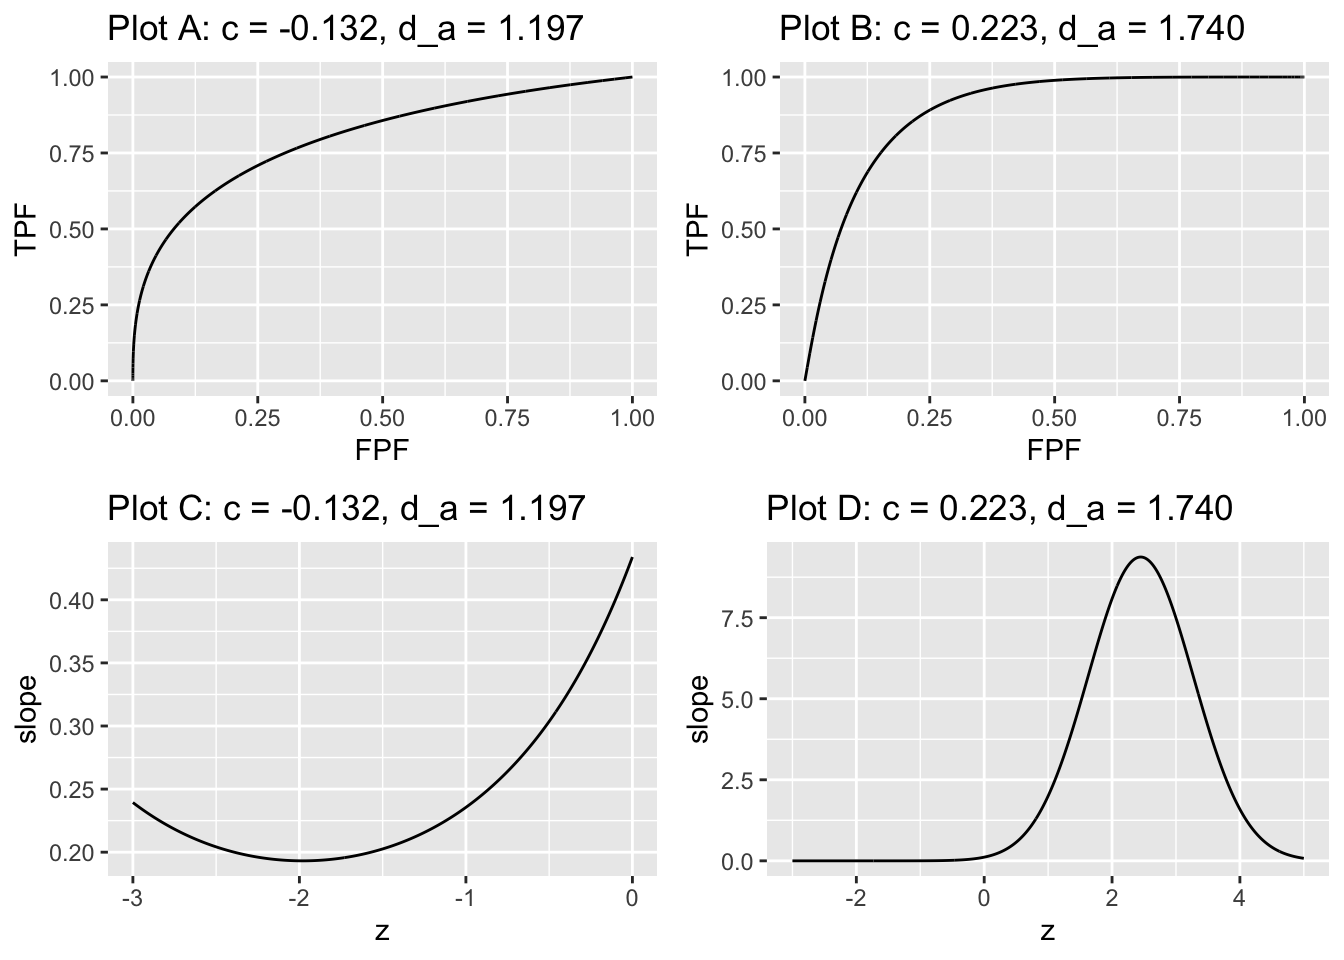
\includegraphics{07-proper-roc-models_files/figure-latex/proper-roc-models-plots-3-1.pdf}
\caption{\label{fig:proper-roc-models-plots-3}The plots are labeled by the values of \(c\) and \(d_a\). Plots A and B are proper ROC plots while plots C and D are the corresponding slope plots. In plot A the slope is infinite near the origin finite at the upper-right corner. In plot B the slope is finite near the origin and zero at the upper-right corner.}
\end{figure}

Plot A is for a negative value of \(c\) which implies \(b < 1\). The slope of the proper ROC is infinite near the origin, corresponding to the very large values of slope in plot C at large likelihood ratio threshold \(\lambda\)), and the slope approaches a non-zero value near the upper right corner of the ROC, corresponding to the non-zero minimum slope in plot C approached as one lowers the likelihood threshold \(\lambda\)).

Plot B is for a positive value of \(c\) which implies \(b > 1\). This time the slope of the ROC near the origin is large but finite, corresponding to the peak in plot D at intermediate likelihood threshold \(\lambda\), and the slope approaches zero near the upper right corner, corresponding to the zero minimum slope in Plot D approached as one lowers the likelihood threshold \(\lambda\) to zero.

To better understand the relation between the ROC plots and the slope plots one moves up the ROC curve by ``slicing'' the slope axis in plots C and D with a downward sliding horizontal cut, i.e., the threshold \(\lambda\) is being lowered starting with a high value. In plot A the slope of the ROC curve starts at the origin with an infinite value corresponding to large slope at the top-right corner in plot C. In plot B the slope of the ROC curve starts at the origin with a finite value corresponding to the finite peak in plot D. Above the peak, there are no solutions for \(z\). The slope decreases monotonically to zero corresponding to the flattening out of the slope at zero for \(z \approx 2\).

Alternatively, one can think of horizontally shrinking each of plots C and D to zero width, and all that remains is the slope axis with a thick vertical line superimposed on it corresponding to the horizontally collapsed curve. In plot C this vertical line extends from positive infinity down to about 0.1 and represents the range of decision variable samples encountered by the observer using the likelihood ratio scale. In plot D this vertical line extends from \(\approx 9.4\) to zero. Values outside of these ranges are not possible for the given parameter values of the underlying binormal model.

The two values of z that can occur for each value of \(\lambda\) implies that the binormal model based proper ROC algorithm has to do a lot of bookkeeping.

\hypertarget{proper-roc-models-cbm}{%
\section{The contaminated binormal model (CBM)}\label{proper-roc-models-cbm}}

The contaminated binormal model \citep{dorfman2000contaminated1, dorfman2000contaminated2, dorfman2000contaminated3}, or CBM, is an alternate model for decision variable sampling in an ROC study. Like the binormal model, it is a two-parameter model, excluding cutoffs. The first parameter is \(\mu_\text{CBM}\), the separation of two unit-variance normal distributions. The sampling for non-diseased cases is from the \(N(0,1)\) distribution, while sampling for diseased cases is from the \(N(\mu_\text{CBM},1)\) distribution, provided the disease is visible, otherwise it is from the \(N(0,1)\) distribution. In other words, for diseased cases the sampling is from a mixture distribution of two unit variance normal distributions, one centered at \(\mu\) and the other centered at 0, with mixing fraction \(\alpha\), the fraction of diseased cases where the abnormality is actually visible. The binning is accomplished, as usual, by the cutoff vector \(\overrightarrow{\zeta}=\left( \zeta_1,...,\zeta_{\text{ROC}-1} \right)\), where \(R_\text{ROC}\) is the number of ROC bins. Defining dummy cutoffs \(\zeta_0=-\infty\) and \(\zeta_{\text{ROC}}=\infty\), the binning rule is as before:

\begin{equation} 
\left.\begin{aligned}
\text{if}~\left (\zeta_{r-1} \le z < \zeta_r  \right ) \text{rating} = r\\
r=1,2,...,R_{ROC} 
\end{aligned}\right\}
\label{eq:proper-roc-models-binning-rule}
\end{equation}

Therefore, CBM is characterized by the parameters \(\mu, \alpha, \overrightarrow{\zeta}\). The parameters \(\mu, \alpha\) can be used to predict the ROC curve and the area under the curve.

\hypertarget{proper-roc-models-cbm-formulae}{%
\subsection{CBM formulae}\label{proper-roc-models-cbm-formulae}}

For non-diseased cases, the \(\text{pdf}\) is the same as for the binormal model:

\begin{equation}
\text{pdf}_N=\phi(z) 
\label{eq:proper-roc-models-cbm-pdfn}
\end{equation}

For diseased cases the \(\text{pdf}\) is a mixture of two unit variance distributions, one centered at zero and the other at \(\mu_\text{CBM}\), with mixing fractions \((1-\alpha)\) and \(\alpha\), respectively:

\begin{equation}
\text{pdf}_D=\left( 1-\alpha \right)\phi(z) + \alpha \phi(z-\mu_\text{CBM})
\label{eq:proper-roc-models-cbm-pdfd}
\end{equation}

The likelihood ratio for the CBM model is given by the ratio of the two pdfs:

\begin{equation}
\left.\begin{aligned}
l_\text{CBM}\left( z|a,b \right)&=\frac{\left( 1-\alpha \right)\phi(z) + \alpha \phi(z-\mu_\text{CBM})}{\phi(z)}\\
&=\left( 1-\alpha \right)+\alpha \, \exp\left(-\frac{\mu_\text{CBM}^2}{2}+z\,\mu_\text{CBM}  \right)
\end{aligned}\right\}
\label{eq:proper-roc-models-cbm-likelihood}
\end{equation}

The function increases monotonically as \(z\) increases which shows that the predicted ROC curve is proper, i.e., its slope decreases monotonically as the operating point moves up the curve (causing both \(z\) and the likelihood ratio to decrease). The slope at the origin (infinite \(z\)) is infinite and the slope at the upper-right corner is \((1-\alpha)\). The predicted ROC coordinates are:

\begin{equation}
\left.\begin{aligned}
\text{FPF}\left( \zeta \right) &= \Phi\left( -\zeta \right)\\
\text{TPF}\left( \zeta \right) &= \left( 1-\alpha \right)\Phi\left( -\zeta \right)+\alpha \,\Phi\left( \mu_\text{CBM}-\zeta \right)
\end{aligned}\right\}
\label{eq:proper-roc-models-cbm-fpf-tpf}
\end{equation}

Since on non-diseased cases the sampling behaviors are identical, the expression for \(\text{FPF}\left( \zeta \right)\) is identical to that for the binormal model: the probability that the z-sample for a non-diseased case exceeds \(\zeta\) is \(\Phi\left( -\zeta \right)\). The second Eqn. \eqref{eq:proper-roc-models-cbm-fpf-tpf} can be understood as follows. \(\text{TPF}\left( \zeta \right)\) is the probability that a diseased case z-sample exceeds \(\zeta\). There are two possibilities: the z-sample arose from the zero-centered distribution, which occurs with probability \(\left( 1-\alpha \right)\), or it arose from the \(\mu_\text{CBM}\)-centered distribution, which occurs with probability \(\alpha\). In the former case, the probability that the z-sample exceeds \(\zeta\) is \(\Phi\left( -\zeta \right)\). In the latter case, the probability is \(\Phi\left( \mu_\text{CBM}-\zeta \right)\). The net probability is the weighted sum of the component probabilities in proportion to their relative frequencies \(\left( 1-\alpha \right):\alpha\).

A similar logic can be used to derive the AUC under the CBM fitted ROC curve:

\begin{equation}
\text{AUC}_\text{CBM}=0.5\left( 1-\alpha \right)+\alpha \,\Phi\left( \frac {\mu_\text{CBM}}{\sqrt{2}} \right)
\label{eq:proper-roc-models-cbm-auc}
\end{equation}

In the limit \(\mu_\text{CBM} \rightarrow \infty\), \(\text{AUC}_\text{CBM} \rightarrow 0.5\left( 1+\alpha \right)\) and in the limit \(\mu_\text{CBM} \rightarrow 0\), \(\text{AUC}_\text{CBM} \rightarrow 0.5\).

\hypertarget{proper-roc-models-cbm-rocs}{%
\subsection{CBM ROC plots}\label{proper-roc-models-cbm-rocs}}

The following figures should further clarify these equations. Fig. \ref{fig:proper-roc-models-cbm-plots-1} shows ROC curves predicted by the CBM model; the values of the \(\alpha\) and \(\mu\) parameters are indicated in the legend. For small \(\alpha\) and/or small \(\mu\) the curve approaches the chance diagonal consistent with the notion that if the lesion is not visible performance can be no better than chance level.

\begin{figure}
\centering
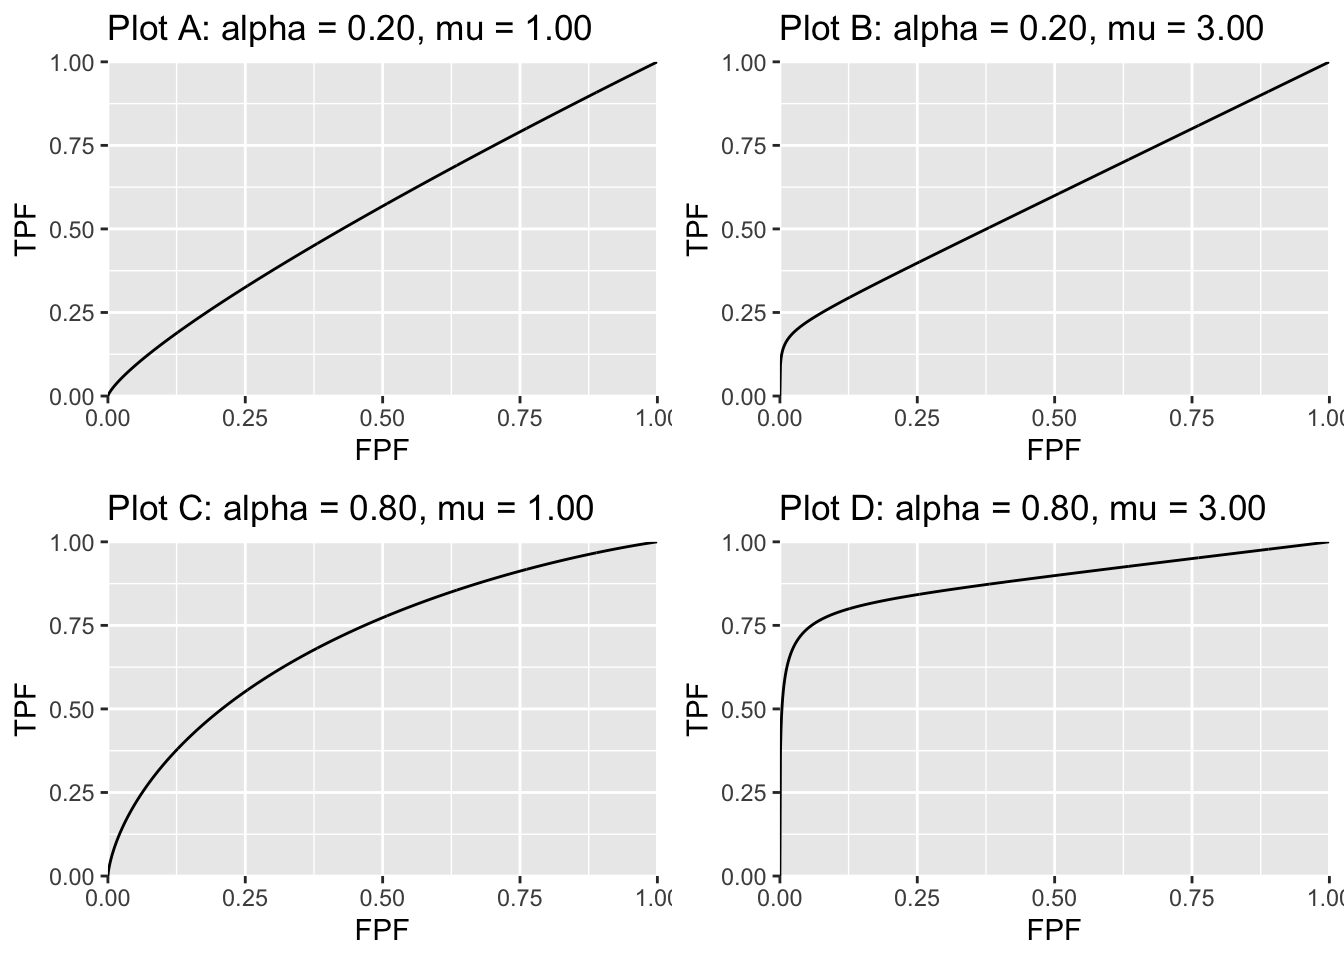
\includegraphics{07-proper-roc-models_files/figure-latex/proper-roc-models-cbm-plots-1-1.pdf}
\caption{\label{fig:proper-roc-models-cbm-plots-1}ROC curves predicted by the CBM model. The corresponding values of the parameters are indicated above the plots. For small \(\alpha\) or small \(\mu\) the curve approaches the chance diagonal, consistent with the notion that if the lesion is not visible, performance can be no better than chance level.}
\end{figure}

As one might expect as \(\mu\) and/or \(\alpha\) increases performance gets better and the curve more closely approaches the top-left corner. The predicted ROC curve is always proper.

The pdf plots are shown next, Fig. \ref{fig:proper-roc-models-cbm-plots-2}.

\hypertarget{proper-roc-models-cbm-pdfs}{%
\subsection{CBM pdf plots}\label{proper-roc-models-cbm-pdfs}}

\begin{figure}
\centering
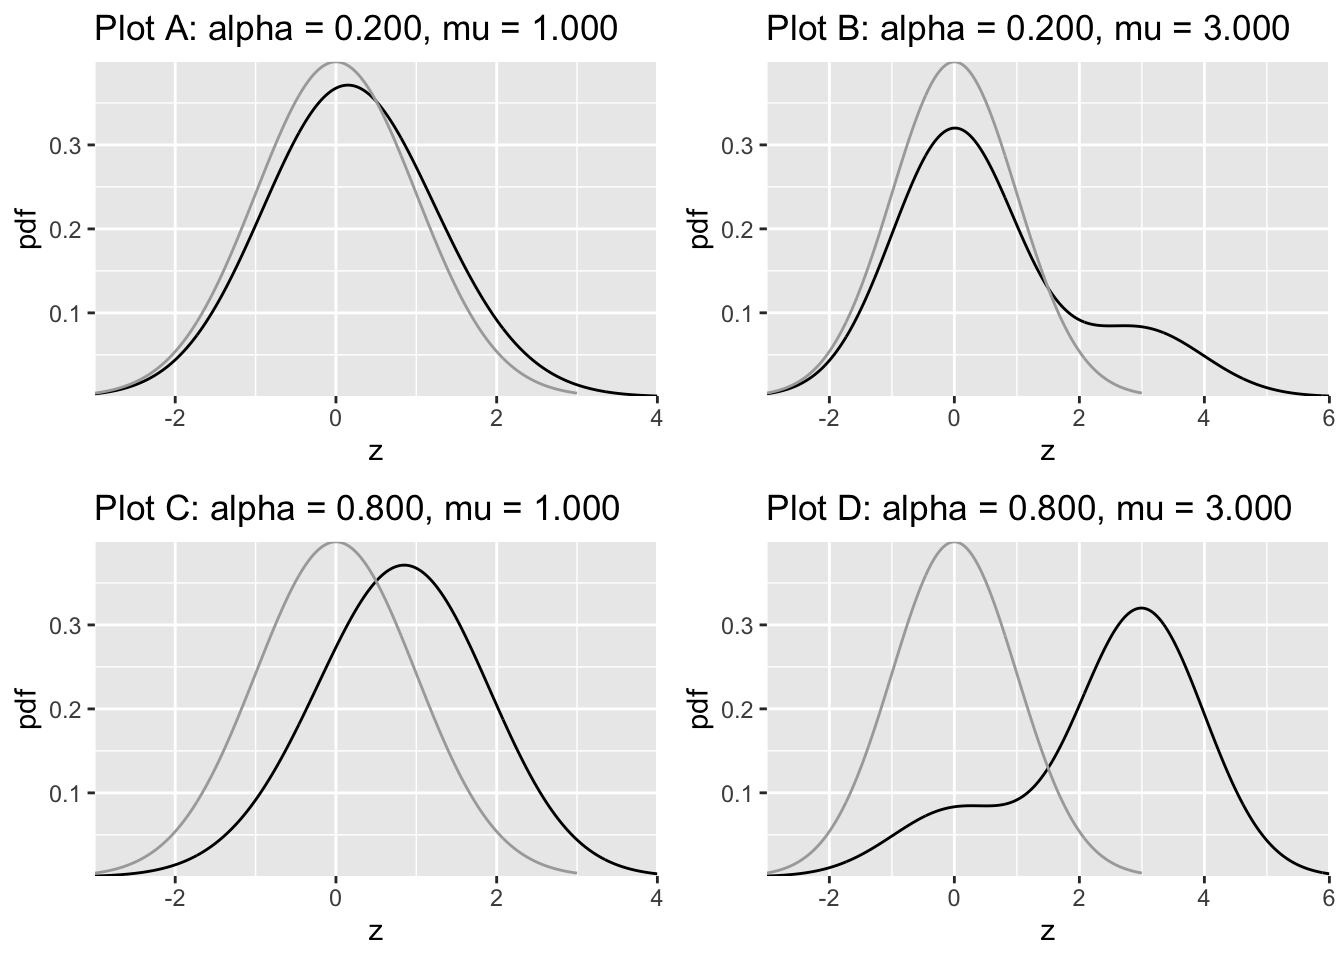
\includegraphics{07-proper-roc-models_files/figure-latex/proper-roc-models-cbm-plots-2-1.pdf}
\caption{\label{fig:proper-roc-models-cbm-plots-2}Density functions predicted by CBM. The dark line is the diseased distribution. The grey line is the non-diseased distribution. The bimodal diseased distribution is clearly evident in plots B and D.}
\end{figure}

Likelihood ratio plots are shown next, Fig. \ref{fig:proper-roc-models-cbm-plots-3}.

\hypertarget{proper-roc-models-cbm-slopes}{%
\subsection{CBM likelihood ratio plots}\label{proper-roc-models-cbm-slopes}}

\begin{figure}
\centering
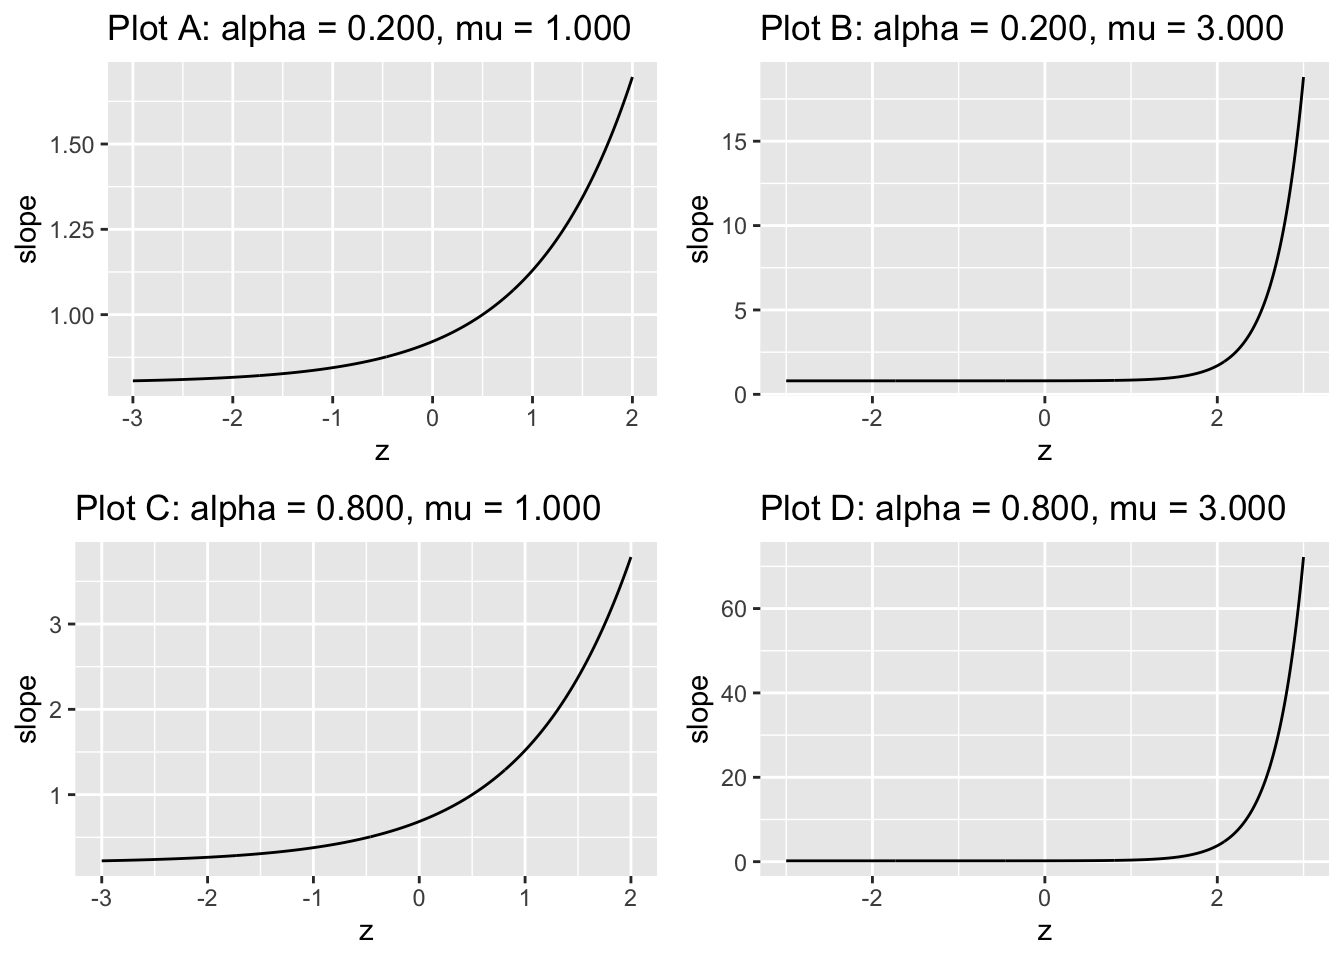
\includegraphics{07-proper-roc-models_files/figure-latex/proper-roc-models-cbm-plots-3-1.pdf}
\caption{\label{fig:proper-roc-models-cbm-plots-3}The slope plots are labeled by the values of \(\alpha\) and \(\mu\). Close examination of the region near the flat part shows it does not plateau at zero; rather the minimum is at \((1 - \alpha)\).}
\end{figure}

All plots are monotonic with \(z\): as \(z\) increases the slope increases. The reader using \(z\) to make decisions, where z is sampled as in the CBM model, is a likelihood ratio observer. In addition, according to TBA Eqn. (20.26), the limiting slope at the upper right corner of the ROC plot approaches \(1-\alpha\) as \(z \rightarrow –\infty\).

\hypertarget{proper-roc-models-bigamma}{%
\section{The bigamma model (BGM)}\label{proper-roc-models-bigamma}}

The bigamma model \citep{dorfman1997proper} was introduced as a way of generating proper ROC curves. It was one of the first successful attempts at this. While of historical importance it nevertheless is interesting in its own right as the decision variable turns out to be a likelihood ratio (which pretty much ensures that the predicted ROC curve will be proper).

\hypertarget{proper-roc-models-bigamma-formulae}{%
\subsection{BGM formulae}\label{proper-roc-models-bigamma-formulae}}

The gamma function is defined by \citep{abramowitz1964handbook}:

\begin{equation}
\Gamma\left( x \right) = \int_{0}^{\infty}t^{x-1}e^{-t} dt
\label{eq:proper-roc-models-gamma}
\end{equation}

A random variable \(X\) has a gamma distribution if its \(\text{pdf}\) is \citep{larsen2005introduction}:

\begin{equation}
\begin{matrix}
f\left( x |r,\lambda\right) = \frac{\lambda^r}{\Gamma\left( r \right)}x^{r-1}e^{-\lambda x}; & 
x\ge 0, r>0, \lambda >0
\end{matrix}
\label{eq:proper-roc-models-gamma-pdf}
\end{equation}

\(1/r\) is called the inverse scale or \emph{rate} parameter and \(r\) is called the \emph{shape} parameter.

The mean and variance of this distribution are given by:

\begin{equation}
\left.\begin{aligned}
E\left( X \right) &= \frac{r}{\lambda} \\
Var\left( X \right) &= \frac{r}{\lambda^2} \\
\end{aligned}\right\}
\label{eq:proper-roc-models-gamma-mean-var}
\end{equation}

The constant-shape bigamma model is defined \citep{dorfman1997proper} by the following pdfs (note \(\lambda = 1\) for the non-diseased pdf and for either pdf \(x \ge 0\)):

\begin{equation}
\left.\begin{aligned}
\text{pdf}_N\left( x \right) &= f\left( x;r,1 \right)\\
&= \frac{1}{\Gamma\left( r \right)}x^{r-1}e^{-x}\\
\text{pdf}_D\left( x \right) &= f\left( x;r,\lambda \right)\\
&= \frac{\lambda^r}{\Gamma\left( r \right)}x^{r-1}e^{-\lambda x} 
\end{aligned}\right\}
\label{eq:proper-roc-models-gamma-pdfs}
\end{equation}

The reason for the name ``bigamma'' is because it involves two gamma distributions (just as ``binormal'' refers to two normal distributions). If the variance of the diseased distribution is to be larger than that of the non-diseased distribution the following constraint must hold:

\begin{equation}
0 < \lambda \le 1
\label{eq:proper-roc-models-bigamma-lambda-inequality}
\end{equation}

The limitation \(x \ge 0\) suggests that \(x\) is equivalent to a likelihood ratio (since the ratio of two pdfs must be non-negative). The model assumes the same shape parameter \(r\) for non-diseased and diseased cases. The likelihood ratio \(l(x)\) is given by:

\begin{equation}
\left.\begin{aligned}
l_\text{BGM}\left( x;r,\lambda \right) &= \frac{\text{pdf}_D\left( x \right)}{\text{pdf}_N\left( x \right)} \\
&=\lambda^r e^{-\left( \lambda - 1 \right) x}
\end{aligned}\right\}
\label{eq:proper-roc-models-bigamma-likelihood}
\end{equation}

``BGM'' stands for bigamma model.

Since the exponential is a monotonic function of its argument the likelihood ratio is a monotonic function of \(x\). A BGM observer basing decisions on observed values of \(x\) exceeding a threshold is a likelihood ratio observer. Notation: note the usage of \(x\) rather than \(z\) as the latter denotes samples from normal distributions. The bigamma model observer bases decisions on the x-sample while the binormal model observer bases decisions on the z-sample. For notational consistency \(\xi\) denotes a threshold on the x-axis and the decision rule is that if \(x \ge \xi\) the case is diagnosed as diseased and otherwise it is diagnosed non-diseased.

Since \(0 < \lambda \le 1\) the slope at the upper right corner of the ROC (corresponding to \(x = 0\)) is \(\lambda ^ r\) and the slope is infinite at the origin (corresponding to \(x = \infty\)). As with PROPROC and CBM, once again one encounters a proper ROC curve approaching the upper-right corner with finite slope. If \(\lambda > 1\) the slope is zero at the origin, which would cause the ROC curve to start out below the chance diagonal. Therefore, constraint \(0 < \lambda \le 1\) is needed not just to yield a wider distribution for diseased cases but to also assure the ROC curve is proper. If \(\lambda = 1\) then regardless of the value of \(r\), the ROC curve is the chance diagonal because the two pdfs become identical.

The cumulative distribution function (CDF) of the gamma distribution is given by:

\begin{equation}
F\left( x;r,\lambda \right) = \int_{0}^{x}f\left( u;r,\lambda \right) du
= \frac{\gamma\left( r, \lambda x \right)}{\Gamma\left( r \right)}
\label{eq:proper-roc-models-gamma-cdf}
\end{equation}

Here the lower incomplete gamma function \citep{abramowitz1964handbook} \(\gamma\left( s,x \right)\) is defined by:

\begin{equation}
\gamma\left( s,x \right) = \int_{0}^{x} t^{s-1} e^{-t} dt
\label{eq:proper-roc-models-gamma-incomplete}
\end{equation}

\texttt{R} implements the CDF of the gamma distribution as \texttt{pgamma()}. The coordinates of the predicted ROC at threshold \(\xi\) are (the complementary probability is needed as FPF and TPF are the probabilities of exceeding a threshold):

\begin{equation}
\left.\begin{aligned}
\text{FPF}\left( \xi|r \right) &= 1 - \frac{\gamma\left( r,\xi \right)}{\Gamma\left( r \right)} \\
&=\int_{\xi}^{\infty} du ~ f\left( u;r,1 \right) \\
\text{TPF}\left( \xi|r, \lambda \right) &= 1 - \frac{\gamma\left( r,\lambda \xi \right)}{\Gamma\left( r \right)} \\
&=\int_{\xi}^{\infty} du ~ f\left( u;r,\lambda \right) \\
\end{aligned}\right\}
\label{eq:proper-roc-models-gamma-fpf-tpf}
\end{equation}

\hypertarget{proper-roc-models-bigamma-rocs}{%
\subsection{BGM ROC plots}\label{proper-roc-models-bigamma-rocs}}

The bigamma-model formulae coded in \texttt{R} were used to generate ROC plots Fig. \ref{fig:proper-roc-models-bigamma-plots-roc}, pdf plots Fig. \ref{fig:proper-roc-models-bigamma-plots-pdf}, and likelihood ratio plots Fig. \ref{fig:proper-roc-models-bigamma-plots-lr} for four pairs of values of the bigamma model parameters \((r, \lambda)\).

\begin{itemize}
\item
  Plot A is for \((r = 1, \lambda = 1)\) when the ROC becomes the chance diagonal; this is actually true regardless of the value of \(r\).
\item
  Plot B is for \((r = 4.39, \lambda = 0.439)\) identical to the values used in \citep{dorfman1997proper} for simulations.
\item
  Plot C is for \((r = 5, \lambda = 0.3)\).
\item
  Plot D is for \((r = 10, \lambda = 0.1)\).
\end{itemize}

\hypertarget{proper-roc-models-bigamma-rocs}{%
\subsection{BGM ROC plots}\label{proper-roc-models-bigamma-rocs}}

\begin{figure}
\centering
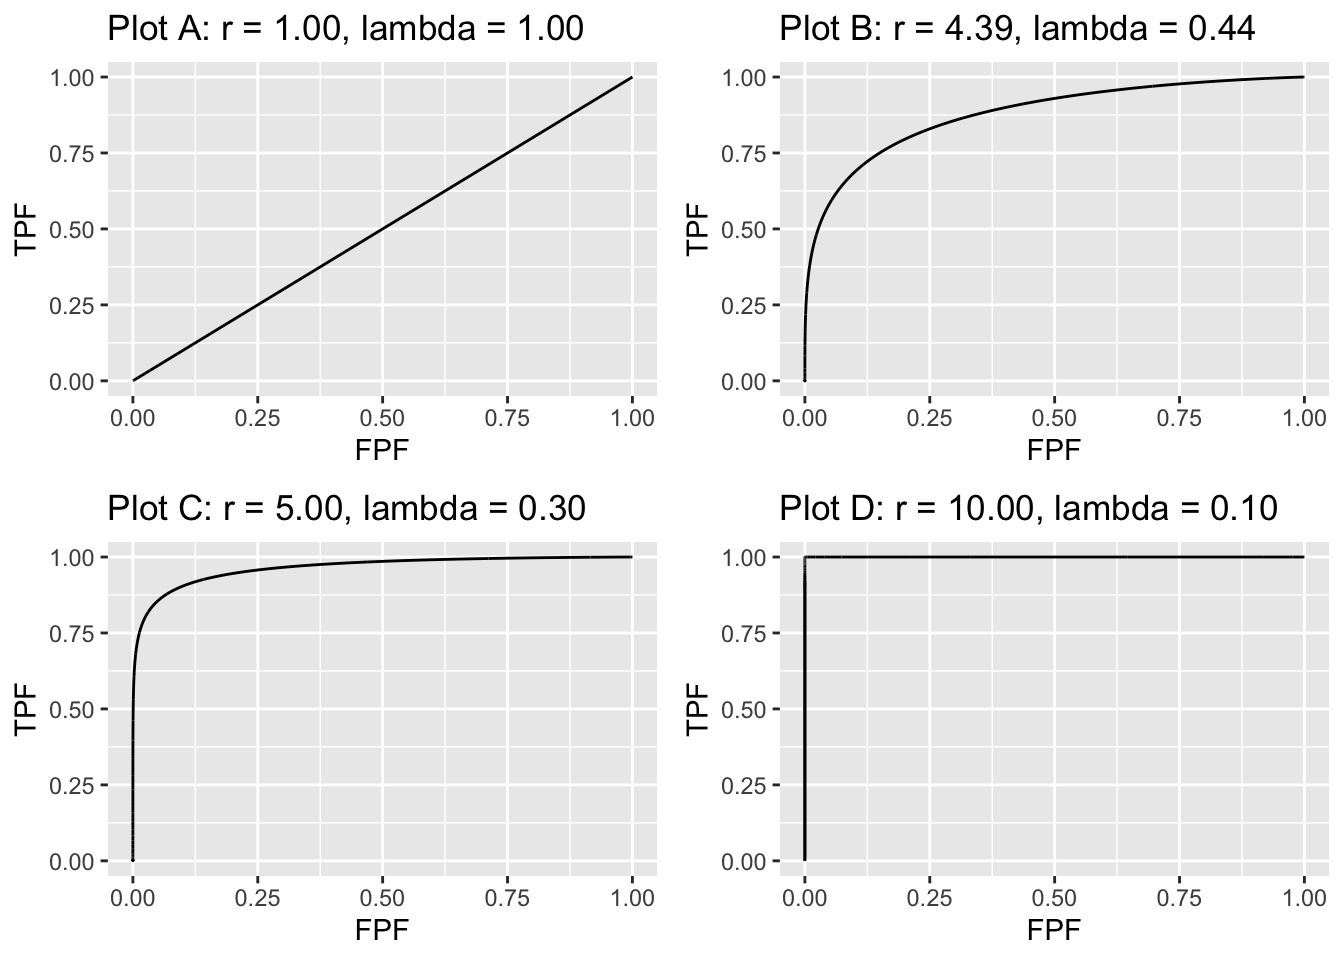
\includegraphics{07-proper-roc-models_files/figure-latex/proper-roc-models-bigamma-plots-roc-1.pdf}
\caption{\label{fig:proper-roc-models-bigamma-plots-roc}ROC curves predicted by the bigamma model. The corresponding AUCs are 0.5, 0.879, 0.965 and 0.9999}
\end{figure}

The reader should check that the slopes in Fig. \ref{fig:proper-roc-models-bigamma-plots-lr} are consistent with the pdfs shown in Fig. \ref{fig:proper-roc-models-bigamma-plots-pdf}. For example, for plot D, the mean of the diseased distribution is 100 relative to 10 for the non-diseased distribution and performance is close to perfect.

I am unaware of an analytic expression for AUC of the bigamma model. However the ROC curve can be numerically integrated. This yields the following values of AUC of the ROCs shown in Fig. \ref{fig:proper-roc-models-bigamma-plots-roc}:

\begin{itemize}
\item
  Plot A: AUC = 0.5;
\item
  Plot B: AUC = 0.8790038;
\item
  Plot C: AUC = 0.9645528;
\item
  Plot D: AUC = 0.9999984.
\end{itemize}

{[}One can confirm that values of \(\lambda > 1\) yield ROC curves below the chance diagonal and AUC less than 0.5. These ROC curves are actually ``reflected'' versions of proper ROC curves; for each such curve the slope starts at a finite positive value near the origin and increases to infinity near the top right corner.{]}

\hypertarget{proper-roc-models-bigamma-pdfs}{%
\subsection{BGM pdf plots}\label{proper-roc-models-bigamma-pdfs}}

\begin{figure}
\centering
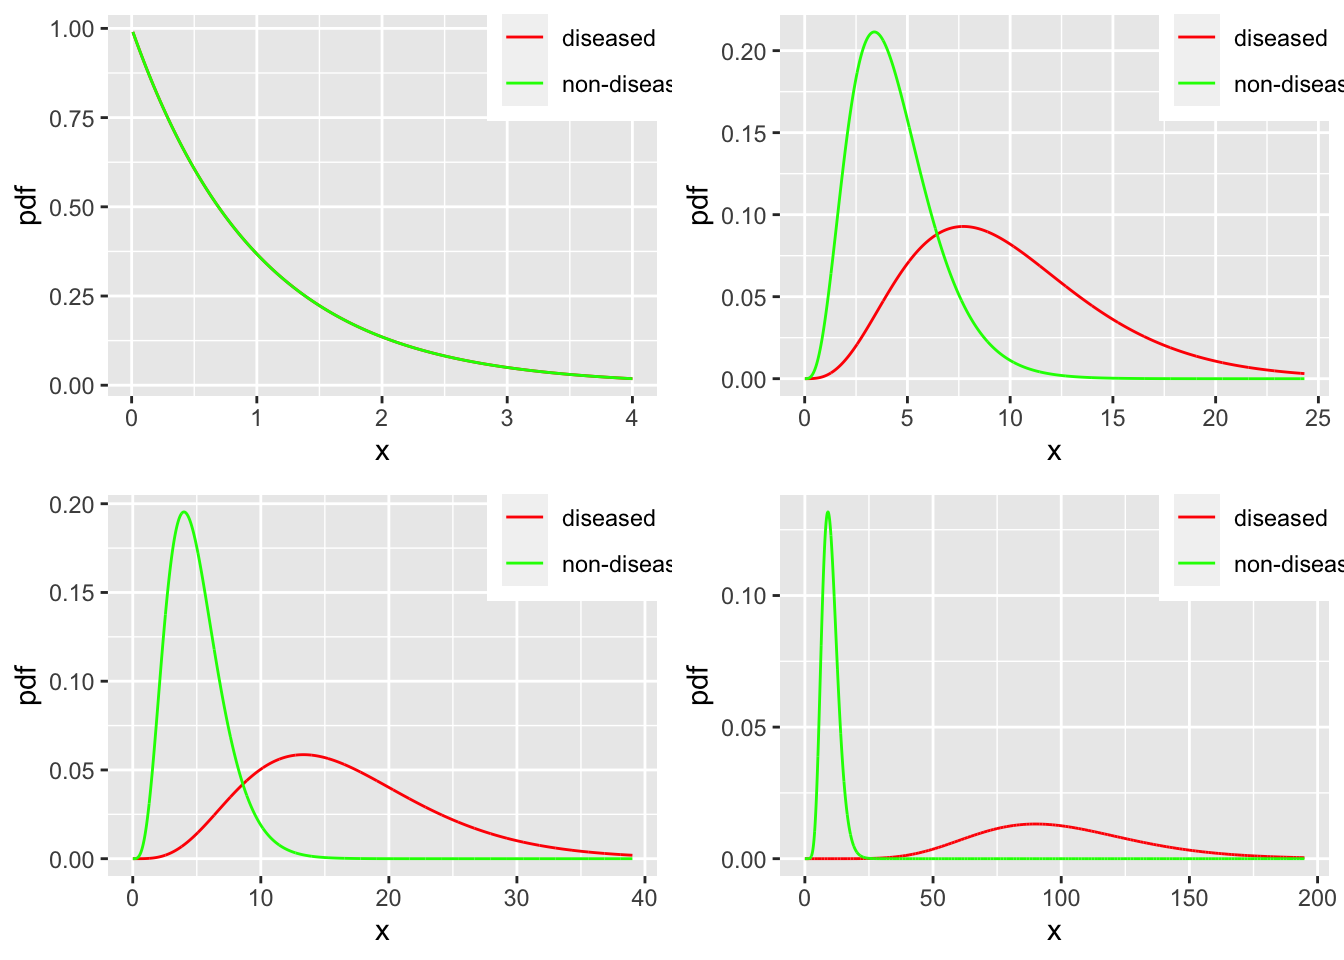
\includegraphics{07-proper-roc-models_files/figure-latex/proper-roc-models-bigamma-plots-pdf-1.pdf}
\caption{\label{fig:proper-roc-models-bigamma-plots-pdf}Density functions predicted by bigamma model. For \(\lambda = 1\) the two pdfs are identical.}
\end{figure}

\hypertarget{proper-roc-models-bigamma-slopes}{%
\subsection{BGM likelihood ratio plots}\label{proper-roc-models-bigamma-slopes}}

\begin{figure}
\centering
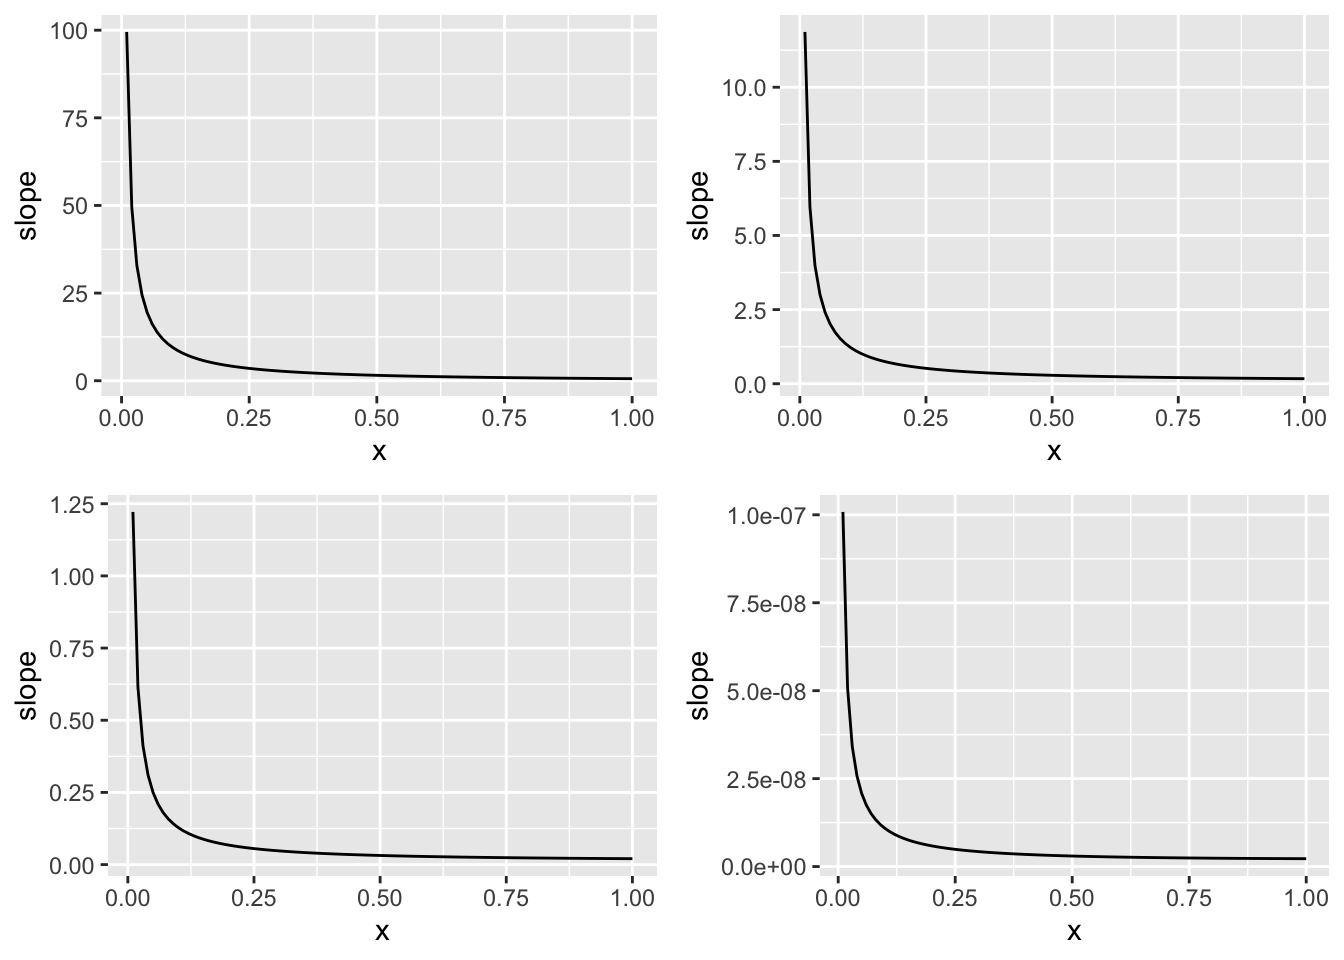
\includegraphics{07-proper-roc-models_files/figure-latex/proper-roc-models-bigamma-plots-lr-1.pdf}
\caption{\label{fig:proper-roc-models-bigamma-plots-lr}Likelihood ratio (or ROC slope) plots predicted by the bigamma model.}
\end{figure}

There used to be software called BIGAMMA, formerly MAXGAM \citep{dorfman1997proper}, implementing the bigamma model, but the University of Iowa ROC website now states ``BIGAMMA is not available for download at this time. Users who desire a proper ROC model should use PROPROC or CBM'' (\url{http://perception.radiology.uiowa.edu}, accessed Apr.~29, 2017).

I understand the de-emphasis of this method since the bigamma distribution is inconsistent with expectations based on the central limit theorem: when many random processes contribute to a measurement the net distribution tends to normality independent of the distributions of the individual processes.

\hypertarget{proper-roc-models-discussion}{%
\section{Discussion}\label{proper-roc-models-discussion}}

With the readily availability of CBM and RSM (both implemented in \texttt{RJafroc}) there is no excuse for not using them. These programs are indeed ``bullet-proof'': they can fit any dataset that one cares to throw at them. The author's preference is to use RSM as it yields additional information about search and lesion-localization performance not available using CBM. PROPOROC has some problems fitting degenerate datasets that can be readily fixed but to my knowledge no one is actively maintaining this important contribution by Prof.~Metz.

\hypertarget{proper-roc-models-metz-eqn-36}{%
\section{Appendix: Metz Eqn 36 numerical check}\label{proper-roc-models-metz-eqn-36}}

The \(c\) and \(d_a\) parameters used here are from an FROC study in breast tomosynthesis \citep{andersson2008breast}. There are two modalities and five readers.

\hypertarget{main-code-and-output}{%
\subsection{Main code and output}\label{main-code-and-output}}

\begin{verbatim}
#>    i j           c        da aucProproc     normDiff
#> 1  1 1 -0.13228036 1.1972393  0.8014164 3.520017e-08
#> 2  1 2 -0.08696513 1.7711756  0.8947898 4.741875e-08
#> 3  1 3 -0.14444185 1.4819349  0.8526605 3.515431e-08
#> 4  1 4  0.08046016 1.5137569  0.8577776 4.971428e-08
#> 5  1 5  0.22255876 1.7401572  0.8909392 2.699855e-08
#> 6  2 1 -0.08174248 0.6281251  0.6716574 2.801793e-08
#> 7  2 2  0.04976448 0.9738786  0.7544739 5.275242e-08
#> 8  2 3 -0.13261262 1.1558707  0.7931787 3.472577e-08
#> 9  2 4  0.11822263 1.6201757  0.8740274 3.922161e-08
#> 10 2 5  0.07810330 0.8928816  0.7360989 3.798459e-08
\end{verbatim}

Note the close correspondence between the formula, Eqn. 36 in \citep{metz1999proper}, and the numerical estimate. Eqn. 31 and Eqn. 36 in the paper (they differ only in parameterizations) are provided without proof -- it was probably obvious to Prof Metz or he wanted to leave it to us ``mere mortals'' to figure it out as a final parting gesture of his legacy. The author once put a significant effort into proving it and even had a bright graduate student from the biostatistics department work on it to no avail. I have observed that these equations always yield very close to the numerical estimates so the theorem is obviously empirically correct, but I have been unable to prove it analytically.

\hypertarget{proper-roc-models-references}{%
\section{Chapter References}\label{proper-roc-models-references}}

\hypertarget{bivariate-binormal-model}{%
\chapter{Bivariate binormal model}\label{bivariate-binormal-model}}

\hypertarget{bivariate-binormal-model-how-much-finished}{%
\section{TBA How much finished}\label{bivariate-binormal-model-how-much-finished}}

20\%

\hypertarget{bivariate-binormal-model-introduction}{%
\section{Introduction}\label{bivariate-binormal-model-introduction}}

Until now, the focus for the ROC paradigm has been on the single rating per case scenario where a single reader interprets a set of cases in a single modality. Of greater clinical interest is a study where a group of readers interprets a common set of cases in multiple modalities. This is because such a study, properly analyzed, yields results that are expected to generalize to the populations of readers and cases from which the study readers and cases were sampled. However, before one can understand several readers interpreting a common case set in multiple modalities, a good place to start is two readers interpreting a common set of cases. Historically, the field progressed from this starting point (the DBMH and ORH analyses methods came after the method to be described here). One might wonder why even bother describing the older approach, since methods for analyzing MRMC datasets have already been described. The analyses methods do not address how to fit the data to models (instead, they assume a figure of merit can be calculated and describe how to perform significance testing using the figure of merit). Data fitting is crucial to understanding factors limiting performance. Before bringing in a three-parameter model like the RSM, addressed in book Chapter 18, it is important to understand the two--parameter model applicable to paired ROC data. The analyst is dealing with two ratings per case, one per reader. An analogous situation applies when one has a single reader interpreting cases in two modalities. The analyst is again faced with two ratings per case, one per modality.

In book Chapter 06 the univariate binormal model was described, which is appropriate for modeling the single rating per case situation (the ``binormal'' comes from the two truth states, not the two modalities). From the previous discussion, it is evident that this needs to be extended to a bivariate model, which would describe studies where each case yields two ratings. Because of the dual interpretations the two ratings per case are correlated. Assuming a 5-rating positive-directed ROC study, on especially easy non-diseased cases the two ratings will both tend to be low (e.g., 1's) and on especially easy diseased cases the two ratings will both tend to be high (e.g., 5's) and on difficult cases, both ratings are likely to be in the ambiguous range (e.g., 3's).

Here is the plan for this chapter. First, the bivariate extension of the univariate binormal model is described. Since most of the readers of this book are expected to not experts in statistics, bivariate sampling will be described at a relatively simple level. Visualization of the resulting probability density functions (pdfs) is demonstrated, which allows the reader to interactively view them, which should allow a better understand of this relatively more complex distribution. Estimation of parameters of the bivariate model from ratings data is addressed. The usage of free software implementing this procedure, i.e., CORROC2, is described. The data format used by CORROC2 is described in some detail as well as how to interpret the program output. \footnote{Since this software runs on Windows, material is provided to allow the user to run it on a MAC (most of this necessary digression, since the author is using OS X, is in TBA Online Appendix 21.D). This digression is not needed in one is using a Windows platform.} Finally, the application of the software to clinical datasets is described. A recent advance that solves degeneracy problems associated with CORROC2 is described, namely CORCBM, for correlated CBM. We conclude with a discussion of the applications of CORROC2.

\hypertarget{bivariate-binormal-model-bivariate-density}{%
\section{Bivariate density function}\label{bivariate-binormal-model-bivariate-density}}

Sampling from the multivariate normal distribution \(N_p\) is as follows:

\begin{equation}
\overrightarrow{x} \sim  N_p\left( \mu, \Sigma \right)
\label{eq:multivariate-sampling-model}
\end{equation}

Here \(\overrightarrow{x}\) is a length \(p\) vector of observed samples, \(\overrightarrow{\mu}\) is a length \(p\) vector containing the means of the multivariate distribution and \(\Sigma\) is the covariance matrix describing the variances, and correlations between the observed samples.

The multivariate normal probability density function \(f_p\left( \overrightarrow{x} ~~ \bigg \rvert ~~\overrightarrow{\mu}, ~~ \overrightarrow{\Sigma} \right)\) is defined by:

\begin{equation} 
f_p\left( \overrightarrow{x} ~~ \bigg \rvert ~~\overrightarrow{\mu}, ~~ \overrightarrow{\Sigma} \right)
= \frac{1}{\left( 2 \pi \right)^{p/2}|\Sigma|^{1/2}}\exp\left( -\frac{\left( \overrightarrow{x}-\overrightarrow{\mu} \right)^T \Sigma^{-1} \left( \overrightarrow{x}-\overrightarrow{\mu} \right)}{2} \right)
\label{eq:bivariate-binormal-model-density-function-multivariate}
\end{equation}

Here \(|\Sigma|\) is the determinant of the matrix and \(T\) is the transpose operator.

For the special case of a bivariate normal distribution, \(p = 2\), this is equivalent to (the subscript 2 is suppressed) \footnote{In the univariate case, \(p = 1\), \(\Sigma\) is replaced by \(\sigma^2\), and the above expression reduces to the pdf of the normal distribution \(N(\mu, \sigma^2)\).}:

\begin{equation} 
f\left( x_1,x_2 ~~ \bigg \rvert ~~ \mu_1, \mu_2,  \sigma_1, \sigma_2, \rho \right)
= \frac{1}{2 \pi \sigma_1 \sigma_2 \sqrt{1-\rho^2}}\exp\left( -\frac{t}{2\left( 1-\rho^2 \right)} \right)
\label{eq:bivariate-binormal-model-density-function}
\end{equation}

where

\begin{equation} 
t=\frac{\left( x_1-\mu_1 \right)^2}{\sigma_1^2}-\frac{2\rho\left( x_1-\mu_1 \right)\left( x_2-\mu_2 \right)}{\sigma_1 \sigma_2}
+\frac{\left( x_2-\mu_2 \right)^2}{\sigma_2^2}
\label{eq:bivariate-binormal-model-density-function2}
\end{equation}

For a bivariate distribution the covariance matrix is:

\begin{equation} 
\Sigma=
\left( \begin{matrix}
\sigma_1^2 & \rho \sigma_1 \sigma_2 \\
\rho \sigma_1 \sigma_2 & 
\sigma_2^2
\end{matrix}
 \right)\label{eq:bivariate-binormal-model-covariance-matrix}
\end{equation}

The \texttt{R} function to evaluate Eqn. \eqref{eq:bivariate-binormal-model-density-function-multivariate} is \texttt{dmvnorm()}, for ``density of multivariate normal distribution'', available via \texttt{R} package \texttt{mvtnorm}. Its usage is illustrated next for the following parameter values:

\begin{equation} 
\left.\begin{aligned}
\overrightarrow{
\mu}&=
\left( \begin{matrix}
\mu_1 \\
\mu_2
\end{matrix}
\right)
=\left( \begin{matrix}
1.5 \\
2.0
\end{matrix}
\right) \\
\sigma_1 &= 1.1 \\
\sigma_2 &= 1.5 \\
\rho &= 0.6 \\
\Sigma&=
\left( 
\begin{matrix}
\sigma_1^2 & \rho \sigma_1 \sigma_2 \\
\rho \sigma_1 \sigma_2  & \sigma_2^2
\end{matrix}\right)
=
\left( 
\begin{matrix}
1.1^2 & 0.6 \times 1.1 \times 1.5 \\
0.6 \times 1.1 \times 1.5  & 1.5^2
\end{matrix}\right)\end{aligned}\right\}
\label{eq:bivariate-binormal-model-parameters}
\end{equation}

In the following code the call to get the pdf occurs at line: \texttt{pdf\ \textless{}-\ dmvnorm(x,\ mean\ =\ c(mu1,mu2),\ sigma\ =\ Sigma)}.

\begin{Shaded}
\begin{Highlighting}[]
\NormalTok{x }\OtherTok{\textless{}{-}} \FunctionTok{c}\NormalTok{(}\FloatTok{0.1}\NormalTok{,}\FloatTok{0.2}\NormalTok{) }\CommentTok{\# the x{-}vector at which to evaluate pdf}
\NormalTok{mu1 }\OtherTok{\textless{}{-}} \FloatTok{1.5} \CommentTok{\# mean modality 1}
\NormalTok{mu2 }\OtherTok{\textless{}{-}} \FloatTok{2.0} \CommentTok{\# mean modality 2}
\NormalTok{var1 }\OtherTok{\textless{}{-}} \FloatTok{1.1}\SpecialCharTok{\^{}}\DecValTok{2}  \CommentTok{\# variance modality 1}
\NormalTok{var2 }\OtherTok{\textless{}{-}} \FloatTok{1.5}\SpecialCharTok{\^{}}\DecValTok{2} \CommentTok{\# variance modality 2}
\NormalTok{rho }\OtherTok{\textless{}{-}} \FloatTok{0.6} \CommentTok{\# correlation between modalities 1 and 2}
\CommentTok{\#}
\CommentTok{\# construct covariance matrix Sigma}
\CommentTok{\# }
\NormalTok{Sigma }\OtherTok{\textless{}{-}} \FunctionTok{matrix}\NormalTok{(}\FunctionTok{c}\NormalTok{(var1, rho}\SpecialCharTok{*}\FunctionTok{sqrt}\NormalTok{(var1}\SpecialCharTok{*}\NormalTok{var2), }
\NormalTok{                  rho}\SpecialCharTok{*}\FunctionTok{sqrt}\NormalTok{(var1}\SpecialCharTok{*}\NormalTok{var2), var2),}\DecValTok{2}\NormalTok{)}
\CommentTok{\#}
\CommentTok{\# pdf }
\CommentTok{\# }
\NormalTok{pdf  }\OtherTok{\textless{}{-}} \FunctionTok{dmvnorm}\NormalTok{(x, }\AttributeTok{mean =} \FunctionTok{c}\NormalTok{(mu1,mu2), }\AttributeTok{sigma =}\NormalTok{ Sigma)}
\CommentTok{\#}
\CommentTok{\# print results}
\CommentTok{\# }
\FunctionTok{cat}\NormalTok{(}\StringTok{"density at x1 = 0.1 and x2 = 0.2 = "}\NormalTok{, pdf, }\StringTok{"}\SpecialCharTok{\textbackslash{}n}\StringTok{"}\NormalTok{)}
\CommentTok{\#\textgreater{} density at x1 = 0.1 and x2 = 0.2 =  0.04622722}
\end{Highlighting}
\end{Shaded}

The parameters describing the bivariate normal distribution are \(\overrightarrow{\mu}\) and \(\Sigma\). The total number of parameters is five: two means, two variances and a correlation coefficient.

\hypertarget{bivariate-binormal-model-formulae}{%
\section{The bivariate binormal model}\label{bivariate-binormal-model-formulae}}

The bivariate binormal model is an extension of the bivariate model just described, to \emph{two truth-states}, non-diseased and diseased, each modeled separately as a bivariate normal distribution. This could potentially result in a doubling of the number of parameters from 5 to 10, but by appropriate shifting and scaling transformations one can ensure that the two means of the bivariate distribution for non-diseased cases are zeroes and the two variances are each unity. This reduces the total number of parameters to 6: \(\mu_1\), \(\mu_2\), \(\sigma_1\), \(\sigma_2\), \(\rho_1\), \(\rho_2\). The bivariate binormal parameters are:

\begin{equation} 
\left.\begin{aligned}
\overrightarrow{
\mu_1}&=
\left( \begin{matrix}
0 \\
0
\end{matrix}
\right)\\
\overrightarrow{
\mu_2}&=
\left( \begin{matrix}
\mu_1 \\
\mu_2
\end{matrix}
\right)\\
\overrightarrow{
\Sigma_1}&=
\left( 
\begin{matrix}
1 & \rho_1 \\
\rho_1  & 1
\end{matrix}
\right) \\
\overrightarrow{
\Sigma_2} &= \left( 
\begin{matrix}
\sigma_1^2 & \rho_2 \sigma_1 \sigma_2 \\
\rho_2 \sigma_1 \sigma_2  & \sigma_2^2
\end{matrix}
\right)
\end{aligned}\right\}
\label{eq:bivariate-binormal-model-all-parameters}
\end{equation}

The decision variable is \(z_{ik_tt}\), where the \(i\) subscript corresponds to the two modalities and the \(t\) subscript corresponds to the two truth states. The correlated ratings pairs \(\left( z_{1k_11},z_{2k_11} \right)\) and \(\left( z_{1k_22},z_{2k_22} \right)\), corresponding to z-samples from non-diseased \(t = 1\) and diseased cases \(t = 2\), respectively, are abbreviated, using vector notation, to \(\overrightarrow{z_{1k_tt}}\) (the vectorized values always ``condense'' the two modalities):

\begin{equation} 
\overrightarrow{z_{k_tt}}=
\left( \begin{matrix}
z_{1k_tt}  \\
z_{2k_tt}
\end{matrix} \right)
\label{eq:bivariate-binormal-model-notation}
\end{equation}

The sampling for each modality, considered in isolation by itself, is as follows (the parameters \(\mu\) and \(\sigma\) are of course modality dependent):

\begin{equation}
\left.\begin{aligned}
z_{k_11} &\sim  N\left( 0, 1 \right) \\
z_{k_22} &\sim  N\left( \mu, \sigma^2 \right)
\end{aligned}\right\}
\label{eq:univariate-binormal-model-sampling}
\end{equation}

Collectively \(\overrightarrow{z_{k_tt}}\) is sampled from \(N_2\left( \overrightarrow{\mu_t}, \Sigma_t \right)\), the bivariate normal distribution with mean \(\overrightarrow{\mu_t}\) and covariance matrix \(\Sigma_t\):

\begin{equation}
\overrightarrow{z_{k_tt}} \sim  N_2\left( \overrightarrow{\mu_t}, \Sigma_t \right)
\label{eq:bivariate-binormal-model-sampling}
\end{equation}

The parameters are truth-state dependent, Eqn. \eqref{eq:bivariate-binormal-model-all-parameters}. In addition one needs to include threshold parameters in the modeling.

For an R-rating single modality ROC task with allowed ratings \(r = 1, 2, ..., \text{R}\), one needs \(\text{R}-1\) thresholds \(\zeta_1,\zeta_2,...,\zeta_{\text{R}-1}\). Defining \(\zeta_0 = -\infty\) and \(\zeta_{\text{R}} = +\infty\) the decision rule is to label a case with rating \(r\) if the realized z-sample satisfies \(\zeta_{r-1} < z \le \zeta_r\).

In the two-modality task the decision variable and the thresholds are modality dependent: i.e., \(z_{ik_tt}\) and \(z_{i'k_tt}\), where \(i \ne i'\) and two sets of thresholds \(\zeta_{i1},\zeta_{i2},...,\zeta_{i (\text{R}-1)}\) and \(\zeta_{i'1},\zeta_{i'2},...,\zeta_{i' (\text{R}-1)}\). As before \(\zeta_{i0} = -\infty\) and \(\zeta_{i'0} = -\infty\) and \(\zeta_{i\text{R}} = +\infty\) and \(\zeta_{i'\text{R}} = +\infty\). The decision rule is to rate a case in modality \(i\) with rating \(r_i\) if \(\zeta_{i(r-1)} < z_i \le \zeta_{ir}\), and the same case in modality \(i'\) is rated \(r_{i'}\) if \(\zeta_{i'(r-1)} < z_{i'} \le \zeta_{i'r}\).

In Eqn. \eqref{eq:bivariate-binormal-model-sampling}, the symbol \(\sim N_2\left( \overrightarrow{\mu_t}, \Sigma_t \right)\) denotes a vector sample of length two from the bivariate normal distribution with mean \(\overrightarrow{\mu_t}\) and covariance matrix \(\Sigma_t\). Each case yields two samples corresponding to the two modalities. The subscript 2 on \(N\) distinguishes the bivariate distribution from the corresponding univariate distribution \(N\) (which has an implicit 1 subscript). For non-diseased cases the Pearson correlation coefficient of the pairs of z-samples is \(\rho_1\) and the corresponding value for diseased cases is \(\rho_2\). The ones along the diagonal of \(\Sigma_1\) confirm that the variances of the two samples for non-diseased cases are individually equal to unity. The corresponding variances for diseased cases are \(\sigma_1^2\) and \(\sigma_2^2\).

The sampling model Eqn. \eqref{eq:bivariate-binormal-model-sampling} is a natural extension to two modalities of the single modality univariate binormal model described in book Chapter 06. The univariate model yields one z-sample per case: samples for non-diseased cases have mean zero and unit variance; samples for diseased cases have mean \(\mu\) and variance \(\sigma^2\). \emph{In contrast the bivariate model yields two z-samples per case. For non-diseased cases the samples have zero mean and unit variance and correlation \(\rho_1\). For diseased cases, the samples for the first modality have mean \(\mu_1\) and variance \(\sigma_1^2\), for the second modality they have mean \(\mu_2\) and variance \(\sigma_2^2\) and their correlation is \(\rho_2\).}

\hypertarget{bivariate-binormal-model-multivariate-density-visualization}{%
\section{Visualizing the bivariate density function}\label{bivariate-binormal-model-multivariate-density-visualization}}

In understanding the bivariate distribution it is helpful to visualize the pdfs. Since one is dealing with a vector \(\overrightarrow{x}\) of length 2, one needs two axes to depict \(x_1\) and \(x_2\) and a third axis to depict the pdf. A sophisticated visualization technique is available for \texttt{R}. The package is called \texttt{plotly}. It is interactive in the sense that by dragging the cursor over the plot one can visualize it from different viewpoints. The following images were captured using this package. Shown in Fig. \ref{fig:bivariate-binormal-model-pdf-plots} are four views of the bivariate distribution density function for \(\mu_{12} = 1.5\), \(\mu_{22} = 2.0\), \(\sigma_1 = 1.0\), \(\sigma_2 = 1.5\), \(\rho_1 = 0.3\) and \(\rho_2 = 0.6\).

\begin{Shaded}
\begin{Highlighting}[]
\NormalTok{x }\OtherTok{\textless{}{-}} \FunctionTok{c}\NormalTok{(}\FloatTok{0.1}\NormalTok{,}\FloatTok{0.2}\NormalTok{) }\CommentTok{\# the x{-}vector at which to evaluate pdf}
\NormalTok{mu1 }\OtherTok{\textless{}{-}} \FloatTok{1.5} \CommentTok{\# diseased mean modality 1}
\NormalTok{mu2 }\OtherTok{\textless{}{-}} \FloatTok{2.0} \CommentTok{\# diseased mean modality 2}
\NormalTok{var1 }\OtherTok{\textless{}{-}} \DecValTok{1}  \CommentTok{\# diseased variance modality 1}
\NormalTok{var2 }\OtherTok{\textless{}{-}}\NormalTok{ (}\FloatTok{1.5}\NormalTok{)}\SpecialCharTok{\^{}}\DecValTok{2} \CommentTok{\# diseased variance modality 2}
\NormalTok{rho1 }\OtherTok{\textless{}{-}} \FloatTok{0.3} \CommentTok{\# non{-}diseased correlation}
\NormalTok{rho2 }\OtherTok{\textless{}{-}} \FloatTok{0.6} \CommentTok{\# diseased correlation}

\CommentTok{\#}
\CommentTok{\# construction the covariance matrix Sigma1 for non{-}diseased}
\CommentTok{\# }
\NormalTok{Sigma1 }\OtherTok{\textless{}{-}} \FunctionTok{matrix}\NormalTok{(}\FunctionTok{c}\NormalTok{(}\DecValTok{1}\NormalTok{, rho1, rho1, var2),}\DecValTok{2}\NormalTok{)}

\CommentTok{\#}
\CommentTok{\# pdf for non{-}diseased}
\CommentTok{\# }
\CommentTok{\# following defaults to zero mean for each modality}
\NormalTok{pdf1  }\OtherTok{\textless{}{-}} \FunctionTok{dmvnorm}\NormalTok{(x, }\AttributeTok{sigma =}\NormalTok{ Sigma1) }

\CommentTok{\#}
\CommentTok{\# construction the covariance matrix Sigma2 for diseased}
\CommentTok{\# }
\NormalTok{Sigma2 }\OtherTok{\textless{}{-}} \FunctionTok{matrix}\NormalTok{(}\FunctionTok{c}\NormalTok{(var1, rho2}\SpecialCharTok{*}\FunctionTok{sqrt}\NormalTok{(var1}\SpecialCharTok{*}\NormalTok{var2), rho2}\SpecialCharTok{*}\FunctionTok{sqrt}\NormalTok{(var1}\SpecialCharTok{*}\NormalTok{var2), var2),}\DecValTok{2}\NormalTok{)}

\CommentTok{\#}
\CommentTok{\# pdf for diseased}
\CommentTok{\# }
\NormalTok{pdf2  }\OtherTok{\textless{}{-}} \FunctionTok{dmvnorm}\NormalTok{(x, }\AttributeTok{mean =} \FunctionTok{c}\NormalTok{(mu1,mu2), }\AttributeTok{sigma =}\NormalTok{ Sigma2)}

\CommentTok{\#}
\CommentTok{\# print results}
\CommentTok{\# }
\FunctionTok{cat}\NormalTok{(}\StringTok{"mu1 ="}\NormalTok{, mu1, }\StringTok{", mu2 ="}\NormalTok{, mu2, }\StringTok{"}\SpecialCharTok{\textbackslash{}n}\StringTok{"}\NormalTok{)}
\CommentTok{\#\textgreater{} mu1 = 1.5 , mu2 = 2}
\FunctionTok{cat}\NormalTok{(}\StringTok{"var1 ="}\NormalTok{, var1, }\StringTok{", var2 ="}\NormalTok{, var2, }\StringTok{"}\SpecialCharTok{\textbackslash{}n}\StringTok{"}\NormalTok{)}
\CommentTok{\#\textgreater{} var1 = 1 , var2 = 2.25}
\FunctionTok{cat}\NormalTok{(}\StringTok{"rho1 ="}\NormalTok{, rho1, }\StringTok{", rho2 ="}\NormalTok{, rho2, }\StringTok{"}\SpecialCharTok{\textbackslash{}n}\StringTok{"}\NormalTok{)}
\CommentTok{\#\textgreater{} rho1 = 0.3 , rho2 = 0.6}
\FunctionTok{cat}\NormalTok{(}\StringTok{"non{-}diseased density at x1 = 0.1 and x2 = 0.2 = "}\NormalTok{, pdf1, }\StringTok{"}\SpecialCharTok{\textbackslash{}n}\StringTok{"}\NormalTok{)}
\CommentTok{\#\textgreater{} non{-}diseased density at x1 = 0.1 and x2 = 0.2 =  0.1070327}
\FunctionTok{cat}\NormalTok{(}\StringTok{"diseased density at x1 = 0.1 and x2 = 0.2 = "}\NormalTok{, pdf2, }\StringTok{"}\SpecialCharTok{\textbackslash{}n}\StringTok{"}\NormalTok{)}
\CommentTok{\#\textgreater{} diseased density at x1 = 0.1 and x2 = 0.2 =  0.04498399}
\end{Highlighting}
\end{Shaded}

\begin{figure}
\centering
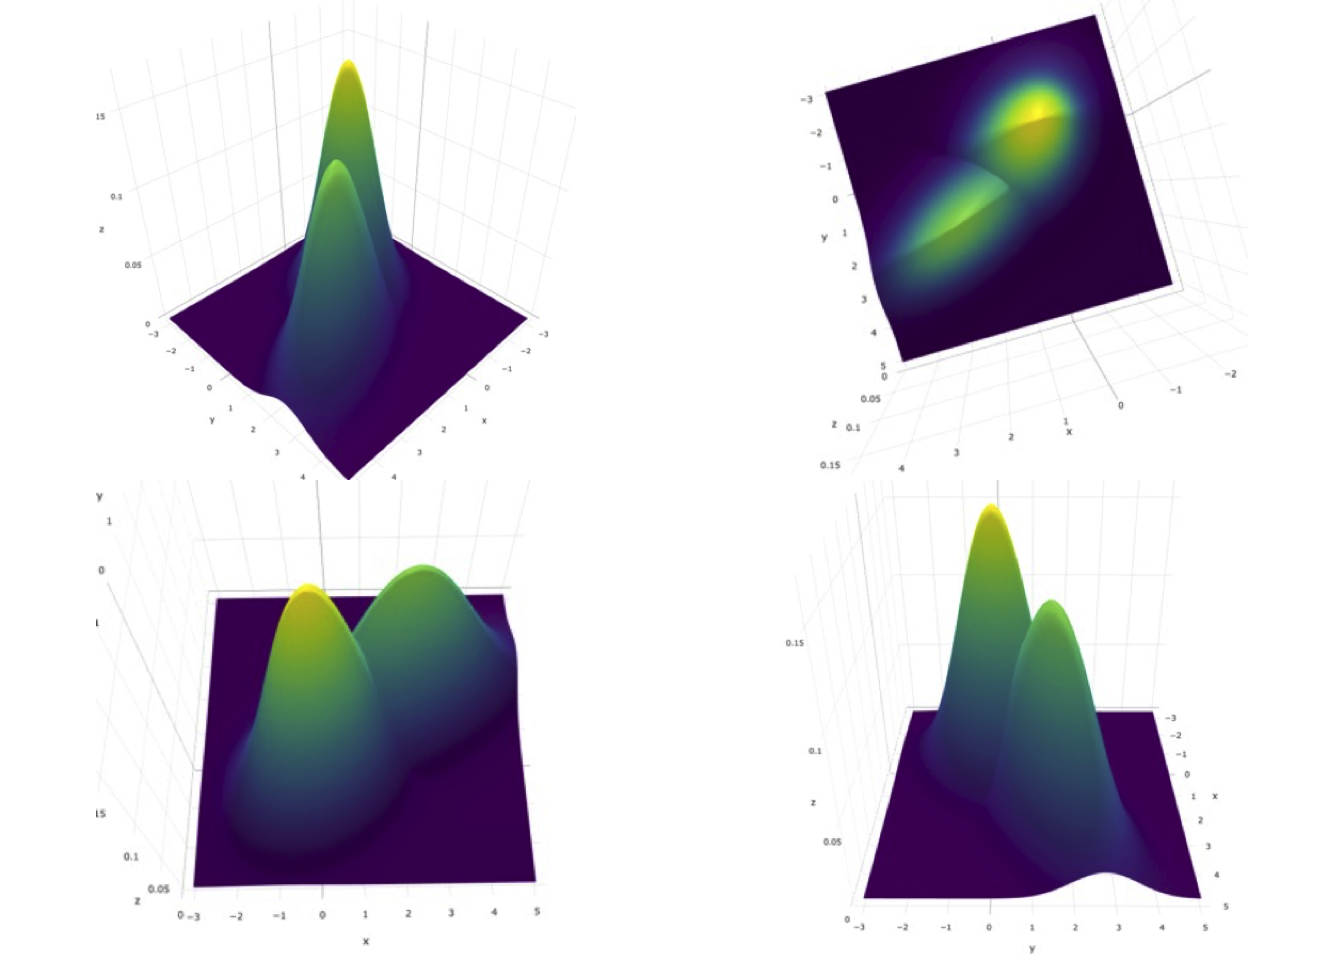
\includegraphics{10-bivariate-binormal-model_files/figure-latex/bivariate-binormal-model-pdf-plots-1.pdf}
\caption{\label{fig:bivariate-binormal-model-pdf-plots}Bivariate pdf plots: Top-left is the default view. Top-right is the `birds eye' view, with the pdf-axis `literally coming at the reader' at right angles to the paper or screen. Bottom-left is the view looking along the y-axis at x = 0. Bottom-right is the view looking along the x-axis at y = 0. The \texttt{R} package \texttt{plotly} was used to capture these screen-shots.}
\end{figure}

\hypertarget{bivariate-binormal-model-multivariate-density-estimation}{%
\section{Estimating bivariate binormal model parameters}\label{bivariate-binormal-model-multivariate-density-estimation}}

In Chapter 06, a method for estimating the parameters of the univariate binormal model for a single-reader single-modality dataset was described. The method involved maximizing the likelihood function, i.e., the probability of the observed data as a function of the model parameters. Specifically, for a 5-rating study, there were four thresholds. The likelihood was a function of six variables: two basic parameters, namely the separation of the two normal distributions and the standard deviation of the diseased distribution relative to the non-diseased distribution. In addition, there are the four thresholds. The threshold parameters are sometimes referred to, in the literature, as nuisance parameters, but nuisance or not, they have to be estimated in order to get to the basic parameters. To estimate the parameters the likelihood function was maximized with respect to these parameters. The values of the parameters yielding the maximum are the maximum-likelihood estimates (MLEs).

With a bivariate model, one is dealing with six basic parameters and threshold parameters corresponding to each modality. The estimation procedure is not fundamentally different, but the presence of the second dimension does complicate the notation. Again, the starting point is the likelihood function, i.e., the probability of the observed data as a function of the parameter values. Since there is a possibility of confusion between the truth index t and the modality index i, each of which ranges from 1 to 2, the non-diseased counts in bin r of the 1st modality and bin s of the 2nd modality is denoted by (i.e., the modality indices occur before the truth index). The corresponding diseased counts are denoted . One needs two indices because each case yields two integer ratings, r and s. Each rating is in the range 1, 2,\ldots, R, where R is the number of ROC bins. It is assumed equal for both modalities. This is not an essential limitation; the method is readily extended, and has been, for unequal numbers of bins in the two modalities. To construct the matrix one starts with a zero-initialized R x R matrix, increment the cell at row \(r\) and column \(s\) of this matrix by unity for each non-diseased case that received a r rating in the 1st modality and an s rating in the 2nd modality. When all non-diseased cases are exhausted, the count in row r and column s of this matrix is ; the procedure is repeated for the diseased cases yielding .

For non-diseased cases, the probability of a z-sample in bin r of the 1st modality and bin s of the 2nd modality is determined by the ``volume'' under the bivariate distribution between modality-1 thresholds and , and between modality-2 thresholds and . Complicated as this may seem, and prior to Alan Genz's work3 showing how to evaluate such multidimensional integrals, this was near impossible, but now it is quite easy, especially in R. The required probability is given by the pmvnorm() function -- this is the generalization to the multivariate case of the pnorm() function, which gives the area under the normal distribution from negative infinity to a specified value. Specifically, pmvnorm()gives the probability under the multivariate distribution between specified thresholds, as illustrated next.

\hypertarget{bivariate-binormal-model-multivariate-density-examples}{%
\section{Examples of bivariate normal probability integrals}\label{bivariate-binormal-model-multivariate-density-examples}}

Needed is the bivariate extension of the univariate cumulative distribution function defined in Eqn. (3.7). Specifically, one needs a way of calculating the integral:

\begin{verbatim}
.   (21.13)
\end{verbatim}

Online Appendix 21.C shows how to do this in R. The code file mainBivariateIntegrals.R implements the ``equation'':

\begin{verbatim}
.   (21.14)
\end{verbatim}

Here \texttt{pmvnorm()} is the integral of the bivariate normal distribution with specified mean and covariance matrix sigma between limits and . The limits are specified by two length-two arrays that are supplied as the first two arguments to this function. The first argument to the function is the concatenated lower thresholds in the two modalities. The second argument is the concatenated upper thresholds in the two modalities. These are followed by the separation parameter vector and the covariance matrix. The function is not limited to two dimensional covariance matrices. With a p x p covariance matrix, the lower and upper limits would each be length p vectors. Here is a bivariate example (p = 2) in mainBivariateIntegrals.R:

\hypertarget{bivariate-binormal-model-multivariate-density-estimation-code}{%
\subsection{Code listing}\label{bivariate-binormal-model-multivariate-density-estimation-code}}

In the last two lines, and . Sourcing the code yields:

\hypertarget{bivariate-binormal-model-examples-integrals}{%
\subsection{Examples of bivariate normal probability integrals}\label{bivariate-binormal-model-examples-integrals}}

The facts that the integral over the entire space yields unity and and that over each half space yields 0.5, and , should make intuitive sense.

\hypertarget{bivariate-binormal-model-likelihood}{%
\section{Likelihood function}\label{bivariate-binormal-model-likelihood}}

The probability of observing and non-diseased and diseased counts, respectively, in bin r in the first modality and bin s in the second modality is:

\begin{verbatim}
.   (21.15)
\end{verbatim}

Including all bins and taking the logarithm, the logarithm of the likelihood function is given by (neglecting a combinatorial factor that does not depend on the parameters):

\begin{verbatim}
.   (21.16)
\end{verbatim}

The maximum likelihood estimates of the parameters are obtained by maximizing the function. This was solved 4,5 by Metz and colleagues more than three decades ago and implemented in software CORROC2. The Metz software is particularly useful as it measures correlations at the underlying z-sample level, which property can be used in designing a data simulator that is matched to a clinical dataset. Much as the author has emphasized that ratings are not numerical quantities, and that the observed ratings are not ``hard'' numbers, the measured correlations are valid, because CORROC2 models the ratings as continuous variables and estimates the correlation based on the bivariate model.

\hypertarget{bivariate-binormal-model-corroc2}{%
\section{CORROC2 software}\label{bivariate-binormal-model-corroc2}}

Around 1980 Prof.~Charles E. Metz and Helen B. Kronman developed software implementing maximum likelihood estimation of the parameters of the bivariate normal model outlined above from data corresponding to two correlated ROC ratings per case. The software is called CORROC2, for ``correlated ROC''. Subsequent revisions to the program were made by Pu-Lan Wang and Jong-Her Shen and more recently by Ben Herman4-7. CORROC2 is used to analyze paired ratings that result when a common set of cases is interpreted under two conditions. The pairing can be simple, as when a single reader interprets a common set of cases in two modalities, or more general as when two different readers interpret a common set of cases in one modality, or when two different readers interpret a common set of cases in two different modalities. The generality makes the method quite useful in a way that, in the judgment of the author, has not been fully exploited to date .

CORROC2 software allows selection of three methods of testing for differences between two conditions.
1. Testing for simultaneous differences between the (a, b) parameters corresponding to two ROC curves.
2. Testing the difference between the binormal-fitted AUCs under two correlated ROCs.
3. Testing the difference between TPFs on two ROC curves at a specified FPF.

To understand the difference between (1) and (2) consider that is that it is possible to have two ROC curves with different shapes but the same fitted AUCs. If the difference in shapes is large enough, method (1) would declare the two conditions different, but method (2) would not. In the examples below, we use method (2).

\hypertarget{bivariate-binormal-model-corroc2-details}{%
\subsection{Details of CORROC2 software}\label{bivariate-binormal-model-corroc2-details}}

This section is one of the few in this book that uses Windows code. If using OS X, one needs to download ``virtual machine'' software as described in Online Appendix 21.D. If using a Windows machine, one does not need to do anything extra. Therefore, in following this chapter it is important that one has either a Windows computer or a Mac computer with a virtual machine installed.

The Windows executable code is named CORROC2.exe. The author downloaded the software, including the Fortran source code, many years ago, ca. 1997, from the University of Chicago website, but it is currently unavailable and unsupported on that site. The author is fortunate that he held onto the downloaded code. The reason is that the FORTRAN source code, with appropriate modifications, can be interfaced to the R code. The currently distributed equivalent code named ROC-kit cannot be run in command-line mode (i.e., without having to use the mouse to select the input file, specify the output file, etc.) The author has confirmed with Mr.~Ben Herman, who is familiar with the code, that by design it cannot be used in command-line mode. The ability to run in command-line mode is needed if one is to call a program from R.

For simplicity, it is assumed that the number of allowed ROC ratings bins, R, is the same in each modality (the software can handle different numbers of ratings in the two modalities). For two modalities, the total number of parameters to be estimated is 6+2(R-1). The six comes from the two means and two variances of the diseased distributions, plus the two correlations (one per truth state) and 2(R-1) from the two sets of thresholds, each with R-1 values. In addition to providing estimates of all parameters of the model, the algorithm provides estimates of the covariance matrix of the parameters. This, not to be confused with , is needed for the same reason it was needed in the univariate case, see Chapter 06: i.e., to estimate variances of the 6-estimates and variances of functions of estimates, e.g., AUC.

\hypertarget{bivariate-binormal-model-corroc2-data-input}{%
\subsection{CORROC2 data input}\label{bivariate-binormal-model-corroc2-data-input}}

Here is a partial example of how the paired ratings data is input to the program (the read-only data file is DataFileInp.txt in the software distribution under software/corrocii/Debug).

TYPICAL EXAMPLE OF 5-CATEGORY DATA --X
5
5
TYPICAL EXAMPLE OF 5-CATEGORY DATA --Y
5
5
4 4
3 5
5 3
1 1
1 1
1 3
1 5

The first line, whose content is immaterial to the analysis, is a description of the data in the 1st modality. The second line (5), is the total number of ratings bins in the 1st modality. The third line (5) is the rating with the highest evidence of disease in the 1st modality (5 in the current example). The fourth line is a description of data in the 2nd modality, again its content is immaterial. The next two fives are the number of bins in the second modality, and the bin number denoting highest evidence of disease in the second modality.

The actual ratings data starts on line 7, which states that the first non-diseased case was rated ROC: 4 in the first modality and ROC: 4 in the second modality. The two ratings for each case, separated by spaces, are input on the same line. Line eight states that the second non-diseased case was rated ROC: 3 in the first modality and ROC: 5 in the second modality, and so on. An asterisk after the last non-diseased case signals the end of the non-diseased cases. The next line has the two ratings corresponding to the first diseased case. Here is a partial example:

4 4
*
4 5
5 5

This says that the first diseased case was rated ROC: 4 in the 1st modality and ROC: 5 in the 2nd modality, the 2nd diseased case was rated ROC: 5 in both modalities, and so on. The last diseased case is followed by another asterisk, and the last line is the word ``area'':

5 5
2 5
*
area

Other choices are available for the last line, but the author will stick to area, which means one wishes to use the area under the binormal-fitted ROC curve as the figure of merit.

\hypertarget{bivariate-binormal-model-corroc2-output}{%
\subsection{CORROC2 output}\label{bivariate-binormal-model-corroc2-output}}

The CORROC2 output associated with this software for the above dataset, 347 lines in all, is in the read-only file DataFileOut.txt, Fig. 21.2 (use RStudio to go down the directory structure and click on the appropriate file; it is displayed, see below, with line numbers):

Fig. 21.2: Lines of CORROC2 output in DataFileOut.txt that are associated with the dataset in DataFileInp.txt.

Condition X and Condition Y denote modalities 1 and 2, respectively . Line 10 of the output summarizes the statistical test to be employed ``AREA (A SUB Z) TEST''. This is because we concluded, line 101, the reader data file DataFileInp.txt with area. Line 13-22 summarizes the dataset, how many ratings, which rating represents greatest evidence of disease, etc. Lines 26 -- 37 summarize the observed ratings matrix for non-diseased cases (labeled ACTUALLY NEGATIVE), i.e., the matrix . For example, there were three cases that were rated s = 3 in CONDITION X and r = 5 in CONDITION Y (the matrix is labeled by its row index, followed by its column index and last with the truth index. The output lists the 5 rating bin as the first row, the 4 rating bin as the second row, etc.). Likewise, lines 40-51 summarize the ratings matrix for diseased cases. Lines 53 -- 59 list the observed operating points in the two modalities, followed by the initial and final estimates of the parameters. The program lists the parameters using the (a,b) notation, not the notation, but one knows how to transform between them: Chapter 06, Eqn. (6.16), and see exercise on conversion below. Here is the output showing the final parameter values (14 values in all):

\begin{verbatim}
            FINAL ESTIMATES OF THE PARAMETERS:
  AX= 1.3006     BX= 0.4919     AY= 1.6049     BY= 0.8704
  R(NEGATIVE CASES)= 0.2599     R(POSITIVE CASES)= 0.4544
  T(I)-0.281  0.221  0.687  1.941
  U(J)-0.791 -0.417  0.175  0.990
\end{verbatim}

Here X refers to condition X and Y to condition Y. AX is the parameter in condition X (what the author calls ). BX is the b parameter in condition X (our ). AY is the parameter in condition Y (i.e., ). BY is the b parameter in condition Y (i.e., ). R(NEGATIVE CASES) is the correlation coefficient for the non-diseased cases (i.e., ). R(POSITIVE CASES) is the correlation coefficient for the diseased cases (i.e., ). Finally, T(I) and U(J) are the thresholds in the two condition, corresponding to and in our notation. Since there are five ratings bins, there are four thresholds in each modality.

Converting the above parameter values to \(\mu, \sigma\) notation

Using the transformations Eqn. (6.16), = 1.3006/0.4919 = 2.644, = 1.844, = 1/.4919 = 2.033, = 1.149, = 0.2599 and = 0.4544 (the correlations are unaffected by linear transformations). Regarding the thresholds, for modality 1, = -0.281/.4919 = -0.571, = 0.221/.4919 = 0.449, etc. Similarly, the thresholds for modality 2 are = -0.791/.8704 = -0.909, = -0.417/.8704 = -0.479, etc. Question for the reader: why were the thresholds divided by the corresponding b-values?

\hypertarget{bivariate-binormal-model-corroc2-covariance-matrix}{%
\subsection{Covariance matrix}\label{bivariate-binormal-model-corroc2-covariance-matrix}}

For convenience of the yet-to-be-described R-program that does all this automatically, the FORTRAN source code was modified to print the elements of the covariance matrix sequentially, i.e., one-per-line. The output corresponding to lines 83 - 280 in file DataFileOut.txt is (shown is a partial listing):

VARIANCE-COVARIANCE MATRIX
14
0.621003E-01
0.205564E-01
0.171881E-01
0.294564E-02
0.104652E-03
-0.684784E-02
0.144067E-01
0.135140E-01
0.127711E-01
0.393710E-02
0.285687E-02
0.285592E-02
0.285248E-02
0.284967E-02
0.205564E-01

The ``14'' is the dimension of each ``edge'' of the 2D covariance matrix, i.e., there are 142 (196) elements in all. The ``14'' comes from the six basic parameters plus the four thresholds in the two conditions. The elements are listed in row-major order, i.e., all the elements of the 1st row, followed by all elements of the 2nd row, etc. One can anticipate some difficulty displaying it, so only the upper-left 6 x 6 corner of the full matrix is shown below, Table 21.1, i.e.~any covariance involving a threshold is not shown. For convenience, the numbers have been rounded to fit and since the matrix is symmetric, there is no need to show numbers below the diagonal:

Table 21.1: This table displays the covariance matrix of the parameters for the dataset in datafileinp.txt. Since the matrix is symmetric, values below the diagonal are not shown. Also not shown are covariance-elements associated with threshold parameters.

.062 .021 .017 .003 .000 -.007

\begin{verbatim}
.022    .002    .002    .001    -.004

    .089    .045    .000    -.010

        .078    .003    -.008

            .026    .000

                .035
\end{verbatim}

The diagonal elements, which represent variances, are all positive.

\hypertarget{bivariate-binormal-model-corroc2-output-restof}{%
\subsection{Rest of CORROC2 output}\label{bivariate-binormal-model-corroc2-output-restof}}

Line 286-320 allows one to plot the ROC curves for the two modalities, but one does not need them, as one knows by now how to generate binormal model predicted curves. Lines 325-327 lists the areas under the respective fitted ROC curves, and their correlation (the is the AUC level correlation, which could be estimated by methods described in Chapter 06):

\begin{verbatim}
        AREA(X)=  0.8784     AREA(Y)=  0.8870
        STD DEV OF AREA(X)=  0.0392     STD DEV OF AREA(Y)=  0.0376
        CORRELATION OF AREA(X) AND AREA(Y) = 0.2569
\end{verbatim}

The remaining lines, 333-341 lists the p-value.

\begin{verbatim}
         STATISTICAL SIGNIFICANCE OF THE DIFFERENCE
  BETWEEN THE TWO CORRELATED ROC CURVES ACCORDING TO THE SELECTED TEST:
\end{verbatim}

\begin{center}\rule{0.5\linewidth}{0.5pt}\end{center}

\begin{verbatim}
THE COMPUTED CORRELATED 'AREA TEST' STATISTIC VALUE IS   -0.1829
WITH A CORRESPONDING TWO-TAILED P-LEVEL OF 0.8549
AND ONE-TAILED P-LEVEL OF 0.4274.
\end{verbatim}

The famed p-value is 0.8549 (it is customary to quote the two-tailed value, see Chapter 08 for details on this). This means that the difference in areas (0.8784 -- 0.8870 = -0.0086) is not statistically significant at Type-I error probability = 0.05. The calculation of the test statistic is described in code mainDiffAzTestStatistic.R. It uses methods described in Chapter 06 to calculate the standard deviation of the difference of two AUCs:

\begin{verbatim}
.   (21.17)
\end{verbatim}

The test -- statistic for determining the significance of the AUC difference is:

\begin{verbatim}
.   (21.18)
\end{verbatim}

\hypertarget{bivariate-binormal-model-corroc2-application}{%
\section{Application to a real dataset}\label{bivariate-binormal-model-corroc2-application}}

Assuming one has set up the connection between the Mac side and the Windows side properly, as described in Online Appendix 21.D, one can apply CORROC2 to real ROC datasets. Open the R file ``mainCorroc2.R'' in the software folder corresponding to this chapter, described in detail in Online Appendix 21.E. Source the file, yielding:

\hypertarget{bivariate-binormal-model-corroc2-application-code-output}{%
\subsection{Code Output}\label{bivariate-binormal-model-corroc2-application-code-output}}

\begin{quote}
source(`\textasciitilde/book2/A ROC analysis/A8 Bivariate binormal model/software/mainCorroc2.R')
\ldots{}
\end{quote}

The 6 parameters are 1.72 0.55 1.87 0.527 0.332 0.798
The 2 sided pValue is 0.482
The covariance matrix is:
{[},1{]} {[},2{]} {[},3{]} {[},4{]} {[},5{]} {[},6{]}
{[}1,{]} 0.120075 0.05096 0.050939 0.01054 6.58e-04 -1.05e-02
{[}2,{]} 0.050956 0.03667 0.013392 0.00550 2.01e-03 -4.87e-03
{[}3,{]} 0.050939 0.01339 0.111921 0.04078 2.28e-04 -1.16e-02
{[}4,{]} 0.010545 0.00550 0.040777 0.02908 1.51e-03 -4.56e-03
{[}5,{]} 0.000658 0.00201 0.000228 0.00151 2.09e-02 3.11e-06
{[}6,{]} -0.010453 -0.00487 -0.011566 -0.00456 3.11e-06 8.67e-03

What the R code does is detailed in Online Appendix 21.D. It reads the file containing the data, the Van Dyke data in the above example, extract the ratings for reader 1 in both modalities, writes the data in the appropriate format for CORROC2, runs the latter program in a Windows environment, reads the resulting output and prints out model parameters and the covariance matrix.

Like most ROC software, the output uses the (a,b) convention, Chapter 06. Recall that in this convention the diseased distribution has unit standard deviation, the non-diseased distribution has standard deviation b, and the separation of the two means is a. Since there are two modalities, there are two a parameters and two b parameters. In the CORROC2 output, the two modalities are referred to as X (1 in our notation) and Y (2 in our notation), respectively, and the ordering of the six parameters is . The ordering also determines the ordering of the covariance matrix. We start with the meanings of the header row and first column of the matrix shown above. The notation {[},1{]} means the first column of the matrix, likewise {[},2{]} is the second column and so on. Likewise, {[}1,{]} means the first row of the matrix, {[}2,{]} means the second row of the matrix, and so on. For example, the above table tells us that the second row and third column of the covariance matrix is 0.013392. This is the covariance between . The diagonal elements of the matrix are the variances. For example, the variance of is 2.09e-02, whose square root is the standard deviation, equal to 0.145.

In the Files panel find the folder named corrocii and open it (you need to click on the name, not the picture of the folder; watch how the folder name is underlined when the cursor is above it, which is RStudio's way of telling you ``yes, it is OK to click here, something will happen''). You should see a number of files with the .FOR extension (these are FORTRAN source code files) and a folder named Debug; click on Debug. Fig. 21.4 is a screen-shot showing the contents of the Debug window. Table 21.2 summarizes the meanings of the files listed in this figure.

\hypertarget{bivariate-binormal-model-corroc2-application-debug-window}{%
\subsection{Contents of the Debug window, as viewed from the Mac side}\label{bivariate-binormal-model-corroc2-application-debug-window}}

Table 21.2: This table summarizes the meanings of the files listed in this Fig. 21.4.
File name Meaning Comment
DataFileInp.txt Input Ratings data in CORROC2 format Read-only file used to illustrate data input format
DataFileOut.txt Output file corresponding to DataFileInp.txt Read-only file used to illustrate the output
1R2MData.txt Ratings data in CORROC2 format Created by RunCorrocOnPairedData.R, line 25
CORROC2.bat Batch file that runs CORROC2.exe See below
CORROC2.exe The actual CORROC2 program\\
CorrocIIinput.txt Input file to the batch file\\
CorrocIIoutput.txt Output file created by batch file

The Windows software is located in software/CORROC2/Debug, Fig. 21.4. CORROC2.bat is a batch file, whose listing follows:
21.7.2: Contents of CORROC2.bat
cd CORROCII
cd Debug
del CorrocIIoutput.txt
CORROC2.exe \textless{} CorrocIIinput.txt \textgreater{} CorrocIIoutput.txt
cd ..
cd ..

The batch file runs on the Windows side. The first two lines change the current directory to corrocii/Debug. The next line deletes the output file, CorrocIIoutput.txt, if it exists. The next line ``pipes'' the contents of CorrocIIinput.txt to the executable file CORROC2.exe and ``pipes'' the output to CorrocIIoutput.txt. The last two lines restore the starting directory. The contents of CorrocIIinput.txt are:

\hypertarget{bivariate-binormal-model-corroc2-application-corrocii-input}{%
\subsection{Contents of CorrocIIinput.txt}\label{bivariate-binormal-model-corroc2-application-corrocii-input}}

y
1R2MData.txt
N
Q

These answer the four questions asked by CORROC2. Try running CORROC2 from the Windows side, Fig. 21.5.

Fig. 21.5: Result of running CORROC2 at the windows 8 command prompt.

The first line of this file is the answer (yes) to the first question asked by CORROC2.exe (you can check these out by clicking on CORROC2.exe in your physical Windows machine or virtual Windows machine): ``Do you want to use data from a previously created input file for the next run?'' The second line is the name of the input file, the third line is the answer (no) to the next question: ``Do you want to save an output file for plotting the ROC curve?'' The reason for the ``no'' is that we are more interested in the screen output, which contains all the estimates, including the covariance matrix, rather than plotting ROC curves. The last line is the answer (``Q'') to the next question asked by CORROC2.exe: ``Do you want to use data from a previously created input file for the next run?(Y/N, or Q for quit)''. Now, in a Windows environment, click on the batch file CORROC2.bat. The latest version of the file CorrocIIoutput.txt should appear in your Explorer window, with the correct date and time stamps. Open this file. The data file is named 1R2MData.txt and if you open it, you will recognize that it is similar to the file used in the section illustrating the data input format for CORROC2. It was created by the R-code.

\hypertarget{bivariate-binormal-model-corroc2-discussion}{%
\section{Discussion / Summary}\label{bivariate-binormal-model-corroc2-discussion}}

CORROC2 is one of the relatively under-utilized tools developed by Prof.~Charles E. Metz. There are only four publications describing it4-6,8 and two of them are difficult to find5,8, nor has the software been maintained on a level comparable to ROCFIT. For example, a method for assessing the goodness of the fit is currently not implemented. With R2 cells, it is almost impossible to maintain greater than five counts per cell, so an alternate method of combining bins has to be implemented.

One reason for the relative underutilization of CORROC2 could be that it is not designed to analyze multiple readers interpreting a common set of cases in two or more modalities i.e., MRMC datasets. For example, in a study in which CORROC2 was used9, four readers interpreted cases in four modalities. With four modalities, there are six possible combinations (4x3/2), so a conservative Bonferroni type correction for the p-value would be to divide 0.05 by 6. For each reader CORROC2 yields a p-value for the difference between the chosen pairs of modalities. If all readers agree, then there is an unambiguous answer, but the method does not allow for correlations between different readers, which undoubtedly leads to loss of power. More fundamentally, it does not address the question of interest: when averaged over all four readers, are the figures of merit in the four modalities different.

It is possible to analyze multiple reader multiple modality MRMC-ROC datasets without actually using CORROC2. In chapters Chapter 09 and Chapter 10, it was shown how one analyzes such datasets using the empirical AUCs. Alternatively, one could estimate AUC using the univariate binormal model software (e.g., ROCFIT, or more modern software). The correlations in the resulting AUC values -- i.e., FOM correlations as distinct from ratings correlations - are explicitly accounted for in the DBMH / ORH analyses, i.e., it is not concerned with ratings correlations. One possible use of CORROC2 would be if one had to compare two CAD algorithms applied to a common dataset, but even here, it is of limited utility since, as a ROC study, location is ignored.

CORROC2 was developed ca. 1980 by Metz, Wang and Kronman 5,10. Subsequent revisions to the program were made by Jong-Her Shen and more recently by Benjamin Herman6,7. Its impact cannot be overstated. There are well in excess of 116 citations to this software. One reason is that, at that time, it was the only software allowing analysis of paired datasets. However, no advances have been made in the intervening 3 decades, which would allow fitting, for example, proper ROC curves to paired - and possibly degenerate - datasets. Part of the reason for this neglect is the shift in emphasis to empirical AUC based analysis, which does not require parametric modeling or curve fitting -- one simply calculates the trapezoidal AUC. However, empirical AUC based analysis has its own limitations, and pursuing an improvement over the parametric approach that removes the current limitations of CORROC2 would, in the author's judgment, quite apart from the specific interest in developing realistic simulators, be of scientific interest.

As a final note, at the time of writing, 4/30/17, an extension of CORROC2 has been published11. It is called CORCBM, for correlated CBM. Details are in a document CORCBM.pdf in the online supplementary material directory corresponding to this chapter. The title of the publication is: ``A bivariate contaminated binormal model for robust fitting of proper ROC curves to a pair of correlated, possibly degenerate, ROC datasets''. It replaces the bivariate binormal model with the bivariate contaminated binormal model; hence its name CORCBM, for correlated CBM. Since CBM was designed to fit practically any single dataset, including degenerate ones, CORCBM is likewise able to fit practically any paired dataset. An application of CORCBM to calibrating a simulator to a data set containing single-modality multiple-reader ratings is described in Chapter 23.

  \bibliography{packages.bib,myRefs.bib}

\end{document}
